\section{Test case four: three agents $-$ two obstacles}

CHANGE

In this case, the initial configurations of the two agents are
$\vect{z}_1 = $ and
$\vect{z}_2 = $.
Their desired configurations in steady-state are
$\vect{z}_{1,des} = $ and
$\vect{z}_{2,des} = $.
The obstacle is placed between the two, at $[0, 2.9]^{\top}$. The time-horizon
length was set to $T_p = 0.5$ sec. The penalty matrices $\mat{Q}$, $\mat{R}$,
$\mat{P}$ were set to $\mat{Q} = 0.5 (I_3 + 0.1 \dagger_3)$,
$\mat{R} = 0.005 I_2$ and $\mat{P} = 0.5 I_3$, where $\dagger_N$ is a
$N \times N$ matrix whose elements are chosen at random between the values $0.0$
and $1.0$.

Trajectory, errors, etc (intro)


%-------------------------------------------------------------------------------
\subsection{Trajectories in 2D}

\noindent\makebox[\linewidth][c]{%
\begin{minipage}{\linewidth}
  \begin{minipage}{0.45\linewidth}
    \begin{figure}[H]
      \scalebox{0.7}{% This file was created by matlab2tikz.
%
%The latest updates can be retrieved from
%  http://www.mathworks.com/matlabcentral/fileexchange/22022-matlab2tikz-matlab2tikz
%where you can also make suggestions and rate matlab2tikz.
%
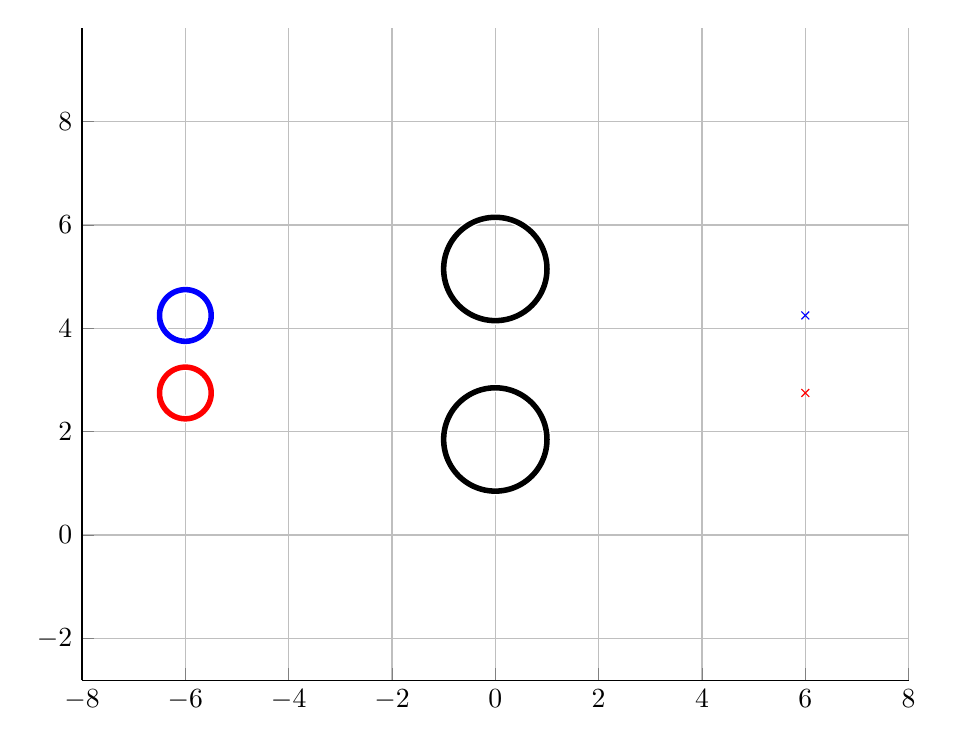
\begin{tikzpicture}

\begin{axis}[%
width=4.133in,
height=3.26in,
at={(0.693in,0.44in)},
scale only axis,
unbounded coords=jump,
xmin=-8,
xmax=8,
xmajorgrids,
ymin=-2.80967741935484,
ymax=9.80967741935484,
ymajorgrids,
axis background/.style={fill=white},
axis x line*=bottom,
axis y line*=left
]
\addplot [color=blue,only marks,mark=x,mark options={solid},forget plot]
  table[row sep=crcr]{%
6	4.25\\
};
\addplot [color=red,only marks,mark=x,mark options={solid},forget plot]
  table[row sep=crcr]{%
6	2.75\\
};
\addplot [color=white,solid,line width=3.0pt,forget plot]
  table[row sep=crcr]{%
-5.5	4.25\\
-5.50030458649045	4.26744974835125\\
-5.50121797487009	4.28487823687206\\
-5.50273905231586	4.30226423163383\\
-5.50486596562921	4.31958655048003\\
-5.5075961234939	4.33682408883347\\
-5.5109261996331	4.35395584540888\\
-5.514852136862	4.37096094779983\\
-5.51936915203084	4.3878186779085\\
-5.52447174185242	4.40450849718747\\
-5.53015368960705	4.42101007166283\\
-5.53640807271661	4.43730329670796\\
-5.5432272711787	4.4533683215379\\
-5.55060297685042	4.46918557339454\\
-5.55852620357054	4.48473578139295\\
-5.56698729810778	4.5\\
-5.57597595192179	4.5149596321166\\
-5.58548121372248	4.52959645173537\\
-5.59549150281253	4.54389262614624\\
-5.60599462319664	4.55783073766283\\
-5.61697777844051	4.57139380484327\\
-5.6284275872613	4.58456530317943\\
-5.64033009983067	4.5973291852295\\
-5.6526708147705	4.60966990016933\\
-5.66543469682057	4.6215724127387\\
-5.67860619515673	4.63302222155949\\
-5.69216926233717	4.64400537680336\\
-5.70610737385376	4.65450849718747\\
-5.72040354826463	4.66451878627752\\
-5.7350403678834	4.67402404807821\\
-5.75	4.68301270189222\\
-5.76526421860705	4.69147379642946\\
-5.78081442660546	4.69939702314958\\
-5.7966316784621	4.7067727288213\\
-5.81269670329204	4.71359192728339\\
-5.82898992833717	4.71984631039295\\
-5.84549150281253	4.72552825814758\\
-5.8621813220915	4.73063084796916\\
-5.87903905220017	4.735147863138\\
-5.89604415459112	4.7390738003669\\
-5.91317591116653	4.7424038765061\\
-5.93041344951997	4.74513403437079\\
-5.94773576836617	4.74726094768414\\
-5.96512176312794	4.74878202512991\\
-5.98255025164875	4.74969541350955\\
-6	4.75\\
-6.01744974835125	4.74969541350955\\
-6.03487823687206	4.74878202512991\\
-6.05226423163383	4.74726094768414\\
-6.06958655048003	4.74513403437079\\
-6.08682408883347	4.7424038765061\\
-6.10395584540888	4.7390738003669\\
-6.12096094779983	4.735147863138\\
-6.1378186779085	4.73063084796916\\
-6.15450849718747	4.72552825814758\\
-6.17101007166283	4.71984631039295\\
-6.18730329670796	4.71359192728339\\
-6.2033683215379	4.7067727288213\\
-6.21918557339454	4.69939702314958\\
-6.23473578139295	4.69147379642946\\
-6.25	4.68301270189222\\
-6.2649596321166	4.67402404807821\\
-6.27959645173537	4.66451878627752\\
-6.29389262614624	4.65450849718747\\
-6.30783073766283	4.64400537680336\\
-6.32139380484327	4.63302222155949\\
-6.33456530317943	4.6215724127387\\
-6.3473291852295	4.60966990016933\\
-6.35966990016933	4.5973291852295\\
-6.3715724127387	4.58456530317943\\
-6.38302222155949	4.57139380484327\\
-6.39400537680336	4.55783073766283\\
-6.40450849718747	4.54389262614624\\
-6.41451878627752	4.52959645173537\\
-6.42402404807821	4.5149596321166\\
-6.43301270189222	4.5\\
-6.44147379642946	4.48473578139295\\
-6.44939702314958	4.46918557339454\\
-6.4567727288213	4.4533683215379\\
-6.46359192728339	4.43730329670796\\
-6.46984631039295	4.42101007166283\\
-6.47552825814758	4.40450849718747\\
-6.48063084796916	4.3878186779085\\
-6.485147863138	4.37096094779983\\
-6.4890738003669	4.35395584540888\\
-6.4924038765061	4.33682408883347\\
-6.49513403437079	4.31958655048003\\
-6.49726094768414	4.30226423163383\\
-6.49878202512991	4.28487823687206\\
-6.49969541350955	4.26744974835125\\
-6.5	4.25\\
-6.49969541350955	4.23255025164875\\
-6.49878202512991	4.21512176312794\\
-6.49726094768414	4.19773576836617\\
-6.49513403437079	4.18041344951997\\
-6.4924038765061	4.16317591116653\\
-6.4890738003669	4.14604415459112\\
-6.485147863138	4.12903905220017\\
-6.48063084796916	4.1121813220915\\
-6.47552825814758	4.09549150281253\\
-6.46984631039295	4.07898992833717\\
-6.46359192728339	4.06269670329204\\
-6.4567727288213	4.0466316784621\\
-6.44939702314958	4.03081442660546\\
-6.44147379642946	4.01526421860705\\
-6.43301270189222	4\\
-6.42402404807821	3.9850403678834\\
-6.41451878627752	3.97040354826463\\
-6.40450849718747	3.95610737385376\\
-6.39400537680336	3.94216926233717\\
-6.38302222155949	3.92860619515673\\
-6.3715724127387	3.91543469682057\\
-6.35966990016933	3.9026708147705\\
-6.3473291852295	3.89033009983067\\
-6.33456530317943	3.8784275872613\\
-6.32139380484327	3.86697777844051\\
-6.30783073766283	3.85599462319664\\
-6.29389262614624	3.84549150281253\\
-6.27959645173537	3.83548121372248\\
-6.2649596321166	3.82597595192179\\
-6.25	3.81698729810778\\
-6.23473578139295	3.80852620357054\\
-6.21918557339454	3.80060297685042\\
-6.2033683215379	3.7932272711787\\
-6.18730329670796	3.78640807271661\\
-6.17101007166283	3.78015368960705\\
-6.15450849718747	3.77447174185242\\
-6.1378186779085	3.76936915203084\\
-6.12096094779983	3.764852136862\\
-6.10395584540888	3.7609261996331\\
-6.08682408883347	3.7575961234939\\
-6.06958655048003	3.75486596562921\\
-6.05226423163383	3.75273905231586\\
-6.03487823687206	3.75121797487009\\
-6.01744974835125	3.75030458649045\\
-6	3.75\\
-5.98255025164875	3.75030458649045\\
-5.96512176312794	3.75121797487009\\
-5.94773576836617	3.75273905231586\\
-5.93041344951997	3.75486596562921\\
-5.91317591116653	3.7575961234939\\
-5.89604415459112	3.7609261996331\\
-5.87903905220017	3.764852136862\\
-5.8621813220915	3.76936915203084\\
-5.84549150281253	3.77447174185242\\
-5.82898992833717	3.78015368960705\\
-5.81269670329204	3.78640807271661\\
-5.7966316784621	3.7932272711787\\
-5.78081442660546	3.80060297685042\\
-5.76526421860705	3.80852620357054\\
-5.75	3.81698729810778\\
-5.7350403678834	3.82597595192179\\
-5.72040354826463	3.83548121372248\\
-5.70610737385376	3.84549150281253\\
-5.69216926233717	3.85599462319664\\
-5.67860619515673	3.86697777844051\\
-5.66543469682057	3.8784275872613\\
-5.6526708147705	3.89033009983067\\
-5.64033009983067	3.9026708147705\\
-5.6284275872613	3.91543469682057\\
-5.61697777844051	3.92860619515673\\
-5.60599462319664	3.94216926233717\\
-5.59549150281253	3.95610737385376\\
-5.58548121372248	3.97040354826463\\
-5.57597595192179	3.9850403678834\\
-5.56698729810778	4\\
-5.55852620357054	4.01526421860705\\
-5.55060297685042	4.03081442660546\\
-5.5432272711787	4.0466316784621\\
-5.53640807271661	4.06269670329204\\
-5.53015368960705	4.07898992833717\\
-5.52447174185242	4.09549150281253\\
-5.51936915203084	4.1121813220915\\
-5.514852136862	4.12903905220017\\
-5.5109261996331	4.14604415459112\\
-5.5075961234939	4.16317591116653\\
-5.50486596562921	4.18041344951997\\
-5.50273905231586	4.19773576836617\\
-5.50121797487009	4.21512176312794\\
-5.50030458649045	4.23255025164875\\
-5.5	4.25\\
nan	nan\\
};
\addplot [color=blue,solid,line width=2.0pt,forget plot]
  table[row sep=crcr]{%
-5.5	4.25\\
-5.50030458649045	4.26744974835125\\
-5.50121797487009	4.28487823687206\\
-5.50273905231586	4.30226423163383\\
-5.50486596562921	4.31958655048003\\
-5.5075961234939	4.33682408883347\\
-5.5109261996331	4.35395584540888\\
-5.514852136862	4.37096094779983\\
-5.51936915203084	4.3878186779085\\
-5.52447174185242	4.40450849718747\\
-5.53015368960705	4.42101007166283\\
-5.53640807271661	4.43730329670796\\
-5.5432272711787	4.4533683215379\\
-5.55060297685042	4.46918557339454\\
-5.55852620357054	4.48473578139295\\
-5.56698729810778	4.5\\
-5.57597595192179	4.5149596321166\\
-5.58548121372248	4.52959645173537\\
-5.59549150281253	4.54389262614624\\
-5.60599462319664	4.55783073766283\\
-5.61697777844051	4.57139380484327\\
-5.6284275872613	4.58456530317943\\
-5.64033009983067	4.5973291852295\\
-5.6526708147705	4.60966990016933\\
-5.66543469682057	4.6215724127387\\
-5.67860619515673	4.63302222155949\\
-5.69216926233717	4.64400537680336\\
-5.70610737385376	4.65450849718747\\
-5.72040354826463	4.66451878627752\\
-5.7350403678834	4.67402404807821\\
-5.75	4.68301270189222\\
-5.76526421860705	4.69147379642946\\
-5.78081442660546	4.69939702314958\\
-5.7966316784621	4.7067727288213\\
-5.81269670329204	4.71359192728339\\
-5.82898992833717	4.71984631039295\\
-5.84549150281253	4.72552825814758\\
-5.8621813220915	4.73063084796916\\
-5.87903905220017	4.735147863138\\
-5.89604415459112	4.7390738003669\\
-5.91317591116653	4.7424038765061\\
-5.93041344951997	4.74513403437079\\
-5.94773576836617	4.74726094768414\\
-5.96512176312794	4.74878202512991\\
-5.98255025164875	4.74969541350955\\
-6	4.75\\
-6.01744974835125	4.74969541350955\\
-6.03487823687206	4.74878202512991\\
-6.05226423163383	4.74726094768414\\
-6.06958655048003	4.74513403437079\\
-6.08682408883347	4.7424038765061\\
-6.10395584540888	4.7390738003669\\
-6.12096094779983	4.735147863138\\
-6.1378186779085	4.73063084796916\\
-6.15450849718747	4.72552825814758\\
-6.17101007166283	4.71984631039295\\
-6.18730329670796	4.71359192728339\\
-6.2033683215379	4.7067727288213\\
-6.21918557339454	4.69939702314958\\
-6.23473578139295	4.69147379642946\\
-6.25	4.68301270189222\\
-6.2649596321166	4.67402404807821\\
-6.27959645173537	4.66451878627752\\
-6.29389262614624	4.65450849718747\\
-6.30783073766283	4.64400537680336\\
-6.32139380484327	4.63302222155949\\
-6.33456530317943	4.6215724127387\\
-6.3473291852295	4.60966990016933\\
-6.35966990016933	4.5973291852295\\
-6.3715724127387	4.58456530317943\\
-6.38302222155949	4.57139380484327\\
-6.39400537680336	4.55783073766283\\
-6.40450849718747	4.54389262614624\\
-6.41451878627752	4.52959645173537\\
-6.42402404807821	4.5149596321166\\
-6.43301270189222	4.5\\
-6.44147379642946	4.48473578139295\\
-6.44939702314958	4.46918557339454\\
-6.4567727288213	4.4533683215379\\
-6.46359192728339	4.43730329670796\\
-6.46984631039295	4.42101007166283\\
-6.47552825814758	4.40450849718747\\
-6.48063084796916	4.3878186779085\\
-6.485147863138	4.37096094779983\\
-6.4890738003669	4.35395584540888\\
-6.4924038765061	4.33682408883347\\
-6.49513403437079	4.31958655048003\\
-6.49726094768414	4.30226423163383\\
-6.49878202512991	4.28487823687206\\
-6.49969541350955	4.26744974835125\\
-6.5	4.25\\
-6.49969541350955	4.23255025164875\\
-6.49878202512991	4.21512176312794\\
-6.49726094768414	4.19773576836617\\
-6.49513403437079	4.18041344951997\\
-6.4924038765061	4.16317591116653\\
-6.4890738003669	4.14604415459112\\
-6.485147863138	4.12903905220017\\
-6.48063084796916	4.1121813220915\\
-6.47552825814758	4.09549150281253\\
-6.46984631039295	4.07898992833717\\
-6.46359192728339	4.06269670329204\\
-6.4567727288213	4.0466316784621\\
-6.44939702314958	4.03081442660546\\
-6.44147379642946	4.01526421860705\\
-6.43301270189222	4\\
-6.42402404807821	3.9850403678834\\
-6.41451878627752	3.97040354826463\\
-6.40450849718747	3.95610737385376\\
-6.39400537680336	3.94216926233717\\
-6.38302222155949	3.92860619515673\\
-6.3715724127387	3.91543469682057\\
-6.35966990016933	3.9026708147705\\
-6.3473291852295	3.89033009983067\\
-6.33456530317943	3.8784275872613\\
-6.32139380484327	3.86697777844051\\
-6.30783073766283	3.85599462319664\\
-6.29389262614624	3.84549150281253\\
-6.27959645173537	3.83548121372248\\
-6.2649596321166	3.82597595192179\\
-6.25	3.81698729810778\\
-6.23473578139295	3.80852620357054\\
-6.21918557339454	3.80060297685042\\
-6.2033683215379	3.7932272711787\\
-6.18730329670796	3.78640807271661\\
-6.17101007166283	3.78015368960705\\
-6.15450849718747	3.77447174185242\\
-6.1378186779085	3.76936915203084\\
-6.12096094779983	3.764852136862\\
-6.10395584540888	3.7609261996331\\
-6.08682408883347	3.7575961234939\\
-6.06958655048003	3.75486596562921\\
-6.05226423163383	3.75273905231586\\
-6.03487823687206	3.75121797487009\\
-6.01744974835125	3.75030458649045\\
-6	3.75\\
-5.98255025164875	3.75030458649045\\
-5.96512176312794	3.75121797487009\\
-5.94773576836617	3.75273905231586\\
-5.93041344951997	3.75486596562921\\
-5.91317591116653	3.7575961234939\\
-5.89604415459112	3.7609261996331\\
-5.87903905220017	3.764852136862\\
-5.8621813220915	3.76936915203084\\
-5.84549150281253	3.77447174185242\\
-5.82898992833717	3.78015368960705\\
-5.81269670329204	3.78640807271661\\
-5.7966316784621	3.7932272711787\\
-5.78081442660546	3.80060297685042\\
-5.76526421860705	3.80852620357054\\
-5.75	3.81698729810778\\
-5.7350403678834	3.82597595192179\\
-5.72040354826463	3.83548121372248\\
-5.70610737385376	3.84549150281253\\
-5.69216926233717	3.85599462319664\\
-5.67860619515673	3.86697777844051\\
-5.66543469682057	3.8784275872613\\
-5.6526708147705	3.89033009983067\\
-5.64033009983067	3.9026708147705\\
-5.6284275872613	3.91543469682057\\
-5.61697777844051	3.92860619515673\\
-5.60599462319664	3.94216926233717\\
-5.59549150281253	3.95610737385376\\
-5.58548121372248	3.97040354826463\\
-5.57597595192179	3.9850403678834\\
-5.56698729810778	4\\
-5.55852620357054	4.01526421860705\\
-5.55060297685042	4.03081442660546\\
-5.5432272711787	4.0466316784621\\
-5.53640807271661	4.06269670329204\\
-5.53015368960705	4.07898992833717\\
-5.52447174185242	4.09549150281253\\
-5.51936915203084	4.1121813220915\\
-5.514852136862	4.12903905220017\\
-5.5109261996331	4.14604415459112\\
-5.5075961234939	4.16317591116653\\
-5.50486596562921	4.18041344951997\\
-5.50273905231586	4.19773576836617\\
-5.50121797487009	4.21512176312794\\
-5.50030458649045	4.23255025164875\\
-5.5	4.25\\
nan	nan\\
};
\addplot [color=white,solid,line width=3.0pt,forget plot]
  table[row sep=crcr]{%
-5.5	2.75\\
-5.50030458649045	2.76744974835125\\
-5.50121797487009	2.78487823687206\\
-5.50273905231586	2.80226423163383\\
-5.50486596562921	2.81958655048003\\
-5.5075961234939	2.83682408883347\\
-5.5109261996331	2.85395584540888\\
-5.514852136862	2.87096094779983\\
-5.51936915203084	2.8878186779085\\
-5.52447174185242	2.90450849718747\\
-5.53015368960705	2.92101007166283\\
-5.53640807271661	2.93730329670796\\
-5.5432272711787	2.9533683215379\\
-5.55060297685042	2.96918557339454\\
-5.55852620357054	2.98473578139295\\
-5.56698729810778	3\\
-5.57597595192179	3.0149596321166\\
-5.58548121372248	3.02959645173537\\
-5.59549150281253	3.04389262614624\\
-5.60599462319664	3.05783073766283\\
-5.61697777844051	3.07139380484327\\
-5.6284275872613	3.08456530317943\\
-5.64033009983067	3.0973291852295\\
-5.6526708147705	3.10966990016933\\
-5.66543469682057	3.1215724127387\\
-5.67860619515673	3.13302222155949\\
-5.69216926233717	3.14400537680336\\
-5.70610737385376	3.15450849718747\\
-5.72040354826463	3.16451878627752\\
-5.7350403678834	3.17402404807821\\
-5.75	3.18301270189222\\
-5.76526421860705	3.19147379642946\\
-5.78081442660546	3.19939702314958\\
-5.7966316784621	3.2067727288213\\
-5.81269670329204	3.21359192728339\\
-5.82898992833717	3.21984631039295\\
-5.84549150281253	3.22552825814758\\
-5.8621813220915	3.23063084796916\\
-5.87903905220017	3.235147863138\\
-5.89604415459112	3.2390738003669\\
-5.91317591116653	3.2424038765061\\
-5.93041344951997	3.24513403437079\\
-5.94773576836617	3.24726094768414\\
-5.96512176312794	3.24878202512991\\
-5.98255025164875	3.24969541350955\\
-6	3.25\\
-6.01744974835125	3.24969541350955\\
-6.03487823687206	3.24878202512991\\
-6.05226423163383	3.24726094768414\\
-6.06958655048003	3.24513403437079\\
-6.08682408883347	3.2424038765061\\
-6.10395584540888	3.2390738003669\\
-6.12096094779983	3.235147863138\\
-6.1378186779085	3.23063084796916\\
-6.15450849718747	3.22552825814758\\
-6.17101007166283	3.21984631039295\\
-6.18730329670796	3.21359192728339\\
-6.2033683215379	3.2067727288213\\
-6.21918557339454	3.19939702314958\\
-6.23473578139295	3.19147379642946\\
-6.25	3.18301270189222\\
-6.2649596321166	3.17402404807821\\
-6.27959645173537	3.16451878627752\\
-6.29389262614624	3.15450849718747\\
-6.30783073766283	3.14400537680336\\
-6.32139380484327	3.13302222155949\\
-6.33456530317943	3.1215724127387\\
-6.3473291852295	3.10966990016933\\
-6.35966990016933	3.0973291852295\\
-6.3715724127387	3.08456530317943\\
-6.38302222155949	3.07139380484327\\
-6.39400537680336	3.05783073766283\\
-6.40450849718747	3.04389262614624\\
-6.41451878627752	3.02959645173537\\
-6.42402404807821	3.0149596321166\\
-6.43301270189222	3\\
-6.44147379642946	2.98473578139295\\
-6.44939702314958	2.96918557339454\\
-6.4567727288213	2.9533683215379\\
-6.46359192728339	2.93730329670796\\
-6.46984631039295	2.92101007166283\\
-6.47552825814758	2.90450849718747\\
-6.48063084796916	2.8878186779085\\
-6.485147863138	2.87096094779983\\
-6.4890738003669	2.85395584540888\\
-6.4924038765061	2.83682408883347\\
-6.49513403437079	2.81958655048003\\
-6.49726094768414	2.80226423163383\\
-6.49878202512991	2.78487823687206\\
-6.49969541350955	2.76744974835125\\
-6.5	2.75\\
-6.49969541350955	2.73255025164875\\
-6.49878202512991	2.71512176312794\\
-6.49726094768414	2.69773576836617\\
-6.49513403437079	2.68041344951997\\
-6.4924038765061	2.66317591116653\\
-6.4890738003669	2.64604415459112\\
-6.485147863138	2.62903905220017\\
-6.48063084796916	2.6121813220915\\
-6.47552825814758	2.59549150281253\\
-6.46984631039295	2.57898992833717\\
-6.46359192728339	2.56269670329204\\
-6.4567727288213	2.5466316784621\\
-6.44939702314958	2.53081442660546\\
-6.44147379642946	2.51526421860705\\
-6.43301270189222	2.5\\
-6.42402404807821	2.4850403678834\\
-6.41451878627752	2.47040354826463\\
-6.40450849718747	2.45610737385376\\
-6.39400537680336	2.44216926233717\\
-6.38302222155949	2.42860619515673\\
-6.3715724127387	2.41543469682057\\
-6.35966990016933	2.4026708147705\\
-6.3473291852295	2.39033009983067\\
-6.33456530317943	2.3784275872613\\
-6.32139380484327	2.36697777844051\\
-6.30783073766283	2.35599462319664\\
-6.29389262614624	2.34549150281253\\
-6.27959645173537	2.33548121372248\\
-6.2649596321166	2.32597595192179\\
-6.25	2.31698729810778\\
-6.23473578139295	2.30852620357054\\
-6.21918557339454	2.30060297685042\\
-6.2033683215379	2.2932272711787\\
-6.18730329670796	2.28640807271661\\
-6.17101007166283	2.28015368960705\\
-6.15450849718747	2.27447174185242\\
-6.1378186779085	2.26936915203084\\
-6.12096094779983	2.264852136862\\
-6.10395584540888	2.2609261996331\\
-6.08682408883347	2.2575961234939\\
-6.06958655048003	2.25486596562921\\
-6.05226423163383	2.25273905231586\\
-6.03487823687206	2.25121797487009\\
-6.01744974835125	2.25030458649045\\
-6	2.25\\
-5.98255025164875	2.25030458649045\\
-5.96512176312794	2.25121797487009\\
-5.94773576836617	2.25273905231586\\
-5.93041344951997	2.25486596562921\\
-5.91317591116653	2.2575961234939\\
-5.89604415459112	2.2609261996331\\
-5.87903905220017	2.264852136862\\
-5.8621813220915	2.26936915203084\\
-5.84549150281253	2.27447174185242\\
-5.82898992833717	2.28015368960705\\
-5.81269670329204	2.28640807271661\\
-5.7966316784621	2.2932272711787\\
-5.78081442660546	2.30060297685042\\
-5.76526421860705	2.30852620357054\\
-5.75	2.31698729810778\\
-5.7350403678834	2.32597595192179\\
-5.72040354826463	2.33548121372248\\
-5.70610737385376	2.34549150281253\\
-5.69216926233717	2.35599462319664\\
-5.67860619515673	2.36697777844051\\
-5.66543469682057	2.3784275872613\\
-5.6526708147705	2.39033009983067\\
-5.64033009983067	2.4026708147705\\
-5.6284275872613	2.41543469682057\\
-5.61697777844051	2.42860619515673\\
-5.60599462319664	2.44216926233717\\
-5.59549150281253	2.45610737385376\\
-5.58548121372248	2.47040354826463\\
-5.57597595192179	2.4850403678834\\
-5.56698729810778	2.5\\
-5.55852620357054	2.51526421860705\\
-5.55060297685042	2.53081442660546\\
-5.5432272711787	2.5466316784621\\
-5.53640807271661	2.56269670329204\\
-5.53015368960705	2.57898992833717\\
-5.52447174185242	2.59549150281253\\
-5.51936915203084	2.6121813220915\\
-5.514852136862	2.62903905220017\\
-5.5109261996331	2.64604415459112\\
-5.5075961234939	2.66317591116653\\
-5.50486596562921	2.68041344951997\\
-5.50273905231586	2.69773576836617\\
-5.50121797487009	2.71512176312794\\
-5.50030458649045	2.73255025164875\\
-5.5	2.75\\
nan	nan\\
};
\addplot [color=red,solid,line width=2.0pt,forget plot]
  table[row sep=crcr]{%
-5.5	2.75\\
-5.50030458649045	2.76744974835125\\
-5.50121797487009	2.78487823687206\\
-5.50273905231586	2.80226423163383\\
-5.50486596562921	2.81958655048003\\
-5.5075961234939	2.83682408883347\\
-5.5109261996331	2.85395584540888\\
-5.514852136862	2.87096094779983\\
-5.51936915203084	2.8878186779085\\
-5.52447174185242	2.90450849718747\\
-5.53015368960705	2.92101007166283\\
-5.53640807271661	2.93730329670796\\
-5.5432272711787	2.9533683215379\\
-5.55060297685042	2.96918557339454\\
-5.55852620357054	2.98473578139295\\
-5.56698729810778	3\\
-5.57597595192179	3.0149596321166\\
-5.58548121372248	3.02959645173537\\
-5.59549150281253	3.04389262614624\\
-5.60599462319664	3.05783073766283\\
-5.61697777844051	3.07139380484327\\
-5.6284275872613	3.08456530317943\\
-5.64033009983067	3.0973291852295\\
-5.6526708147705	3.10966990016933\\
-5.66543469682057	3.1215724127387\\
-5.67860619515673	3.13302222155949\\
-5.69216926233717	3.14400537680336\\
-5.70610737385376	3.15450849718747\\
-5.72040354826463	3.16451878627752\\
-5.7350403678834	3.17402404807821\\
-5.75	3.18301270189222\\
-5.76526421860705	3.19147379642946\\
-5.78081442660546	3.19939702314958\\
-5.7966316784621	3.2067727288213\\
-5.81269670329204	3.21359192728339\\
-5.82898992833717	3.21984631039295\\
-5.84549150281253	3.22552825814758\\
-5.8621813220915	3.23063084796916\\
-5.87903905220017	3.235147863138\\
-5.89604415459112	3.2390738003669\\
-5.91317591116653	3.2424038765061\\
-5.93041344951997	3.24513403437079\\
-5.94773576836617	3.24726094768414\\
-5.96512176312794	3.24878202512991\\
-5.98255025164875	3.24969541350955\\
-6	3.25\\
-6.01744974835125	3.24969541350955\\
-6.03487823687206	3.24878202512991\\
-6.05226423163383	3.24726094768414\\
-6.06958655048003	3.24513403437079\\
-6.08682408883347	3.2424038765061\\
-6.10395584540888	3.2390738003669\\
-6.12096094779983	3.235147863138\\
-6.1378186779085	3.23063084796916\\
-6.15450849718747	3.22552825814758\\
-6.17101007166283	3.21984631039295\\
-6.18730329670796	3.21359192728339\\
-6.2033683215379	3.2067727288213\\
-6.21918557339454	3.19939702314958\\
-6.23473578139295	3.19147379642946\\
-6.25	3.18301270189222\\
-6.2649596321166	3.17402404807821\\
-6.27959645173537	3.16451878627752\\
-6.29389262614624	3.15450849718747\\
-6.30783073766283	3.14400537680336\\
-6.32139380484327	3.13302222155949\\
-6.33456530317943	3.1215724127387\\
-6.3473291852295	3.10966990016933\\
-6.35966990016933	3.0973291852295\\
-6.3715724127387	3.08456530317943\\
-6.38302222155949	3.07139380484327\\
-6.39400537680336	3.05783073766283\\
-6.40450849718747	3.04389262614624\\
-6.41451878627752	3.02959645173537\\
-6.42402404807821	3.0149596321166\\
-6.43301270189222	3\\
-6.44147379642946	2.98473578139295\\
-6.44939702314958	2.96918557339454\\
-6.4567727288213	2.9533683215379\\
-6.46359192728339	2.93730329670796\\
-6.46984631039295	2.92101007166283\\
-6.47552825814758	2.90450849718747\\
-6.48063084796916	2.8878186779085\\
-6.485147863138	2.87096094779983\\
-6.4890738003669	2.85395584540888\\
-6.4924038765061	2.83682408883347\\
-6.49513403437079	2.81958655048003\\
-6.49726094768414	2.80226423163383\\
-6.49878202512991	2.78487823687206\\
-6.49969541350955	2.76744974835125\\
-6.5	2.75\\
-6.49969541350955	2.73255025164875\\
-6.49878202512991	2.71512176312794\\
-6.49726094768414	2.69773576836617\\
-6.49513403437079	2.68041344951997\\
-6.4924038765061	2.66317591116653\\
-6.4890738003669	2.64604415459112\\
-6.485147863138	2.62903905220017\\
-6.48063084796916	2.6121813220915\\
-6.47552825814758	2.59549150281253\\
-6.46984631039295	2.57898992833717\\
-6.46359192728339	2.56269670329204\\
-6.4567727288213	2.5466316784621\\
-6.44939702314958	2.53081442660546\\
-6.44147379642946	2.51526421860705\\
-6.43301270189222	2.5\\
-6.42402404807821	2.4850403678834\\
-6.41451878627752	2.47040354826463\\
-6.40450849718747	2.45610737385376\\
-6.39400537680336	2.44216926233717\\
-6.38302222155949	2.42860619515673\\
-6.3715724127387	2.41543469682057\\
-6.35966990016933	2.4026708147705\\
-6.3473291852295	2.39033009983067\\
-6.33456530317943	2.3784275872613\\
-6.32139380484327	2.36697777844051\\
-6.30783073766283	2.35599462319664\\
-6.29389262614624	2.34549150281253\\
-6.27959645173537	2.33548121372248\\
-6.2649596321166	2.32597595192179\\
-6.25	2.31698729810778\\
-6.23473578139295	2.30852620357054\\
-6.21918557339454	2.30060297685042\\
-6.2033683215379	2.2932272711787\\
-6.18730329670796	2.28640807271661\\
-6.17101007166283	2.28015368960705\\
-6.15450849718747	2.27447174185242\\
-6.1378186779085	2.26936915203084\\
-6.12096094779983	2.264852136862\\
-6.10395584540888	2.2609261996331\\
-6.08682408883347	2.2575961234939\\
-6.06958655048003	2.25486596562921\\
-6.05226423163383	2.25273905231586\\
-6.03487823687206	2.25121797487009\\
-6.01744974835125	2.25030458649045\\
-6	2.25\\
-5.98255025164875	2.25030458649045\\
-5.96512176312794	2.25121797487009\\
-5.94773576836617	2.25273905231586\\
-5.93041344951997	2.25486596562921\\
-5.91317591116653	2.2575961234939\\
-5.89604415459112	2.2609261996331\\
-5.87903905220017	2.264852136862\\
-5.8621813220915	2.26936915203084\\
-5.84549150281253	2.27447174185242\\
-5.82898992833717	2.28015368960705\\
-5.81269670329204	2.28640807271661\\
-5.7966316784621	2.2932272711787\\
-5.78081442660546	2.30060297685042\\
-5.76526421860705	2.30852620357054\\
-5.75	2.31698729810778\\
-5.7350403678834	2.32597595192179\\
-5.72040354826463	2.33548121372248\\
-5.70610737385376	2.34549150281253\\
-5.69216926233717	2.35599462319664\\
-5.67860619515673	2.36697777844051\\
-5.66543469682057	2.3784275872613\\
-5.6526708147705	2.39033009983067\\
-5.64033009983067	2.4026708147705\\
-5.6284275872613	2.41543469682057\\
-5.61697777844051	2.42860619515673\\
-5.60599462319664	2.44216926233717\\
-5.59549150281253	2.45610737385376\\
-5.58548121372248	2.47040354826463\\
-5.57597595192179	2.4850403678834\\
-5.56698729810778	2.5\\
-5.55852620357054	2.51526421860705\\
-5.55060297685042	2.53081442660546\\
-5.5432272711787	2.5466316784621\\
-5.53640807271661	2.56269670329204\\
-5.53015368960705	2.57898992833717\\
-5.52447174185242	2.59549150281253\\
-5.51936915203084	2.6121813220915\\
-5.514852136862	2.62903905220017\\
-5.5109261996331	2.64604415459112\\
-5.5075961234939	2.66317591116653\\
-5.50486596562921	2.68041344951997\\
-5.50273905231586	2.69773576836617\\
-5.50121797487009	2.71512176312794\\
-5.50030458649045	2.73255025164875\\
-5.5	2.75\\
nan	nan\\
};
\addplot [color=white,solid,line width=3.0pt,forget plot]
  table[row sep=crcr]{%
1	1.85\\
0.999390827019096	1.8848994967025\\
0.997564050259824	1.91975647374413\\
0.994521895368273	1.95452846326765\\
0.99026806874157	1.98917310096007\\
0.984807753012208	2.02364817766693\\
0.978147600733806	2.05791169081776\\
0.970295726275996	2.09192189559967\\
0.961261695938319	2.125637355817\\
0.951056516295154	2.15901699437495\\
0.939692620785908	2.19202014332567\\
0.927183854566787	2.22460659341591\\
0.913545457642601	2.2567366430758\\
0.898794046299167	2.28837114678908\\
0.882947592858927	2.31947156278589\\
0.866025403784439	2.35\\
0.848048096156426	2.37991926423321\\
0.829037572555042	2.40919290347075\\
0.809016994374947	2.43778525229247\\
0.788010753606722	2.46566147532566\\
0.766044443118978	2.49278760968654\\
0.743144825477394	2.51913060635886\\
0.719339800338651	2.544658370459\\
0.694658370458997	2.56933980033865\\
0.669130606358858	2.59314482547739\\
0.642787609686539	2.61604444311898\\
0.615661475325658	2.63801075360672\\
0.587785252292473	2.65901699437495\\
0.559192903470747	2.67903757255504\\
0.529919264233205	2.69804809615643\\
0.5	2.71602540378444\\
0.469471562785891	2.73294759285893\\
0.438371146789077	2.74879404629917\\
0.4067366430758	2.7635454576426\\
0.374606593415912	2.77718385456679\\
0.342020143325669	2.78969262078591\\
0.309016994374947	2.80105651629515\\
0.275637355816999	2.81126169593832\\
0.241921895599668	2.820295726276\\
0.207911690817759	2.82814760073381\\
0.17364817766693	2.83480775301221\\
0.139173100960066	2.84026806874157\\
0.104528463267653	2.84452189536827\\
0.0697564737441255	2.84756405025982\\
0.0348994967025011	2.8493908270191\\
6.12323399573677e-17	2.85\\
-0.0348994967025007	2.8493908270191\\
-0.0697564737441253	2.84756405025982\\
-0.104528463267653	2.84452189536827\\
-0.139173100960065	2.84026806874157\\
-0.17364817766693	2.83480775301221\\
-0.207911690817759	2.82814760073381\\
-0.241921895599668	2.820295726276\\
-0.275637355816999	2.81126169593832\\
-0.309016994374947	2.80105651629515\\
-0.342020143325669	2.78969262078591\\
-0.374606593415912	2.77718385456679\\
-0.4067366430758	2.7635454576426\\
-0.438371146789078	2.74879404629917\\
-0.469471562785891	2.73294759285893\\
-0.5	2.71602540378444\\
-0.529919264233205	2.69804809615643\\
-0.559192903470747	2.67903757255504\\
-0.587785252292473	2.65901699437495\\
-0.615661475325658	2.63801075360672\\
-0.642787609686539	2.61604444311898\\
-0.669130606358858	2.59314482547739\\
-0.694658370458997	2.56933980033865\\
-0.719339800338651	2.544658370459\\
-0.743144825477394	2.51913060635886\\
-0.766044443118978	2.49278760968654\\
-0.788010753606722	2.46566147532566\\
-0.809016994374947	2.43778525229247\\
-0.829037572555042	2.40919290347075\\
-0.848048096156426	2.37991926423321\\
-0.866025403784439	2.35\\
-0.882947592858927	2.31947156278589\\
-0.898794046299167	2.28837114678908\\
-0.913545457642601	2.2567366430758\\
-0.927183854566787	2.22460659341591\\
-0.939692620785908	2.19202014332567\\
-0.951056516295154	2.15901699437495\\
-0.961261695938319	2.125637355817\\
-0.970295726275996	2.09192189559967\\
-0.978147600733806	2.05791169081776\\
-0.984807753012208	2.02364817766693\\
-0.99026806874157	1.98917310096007\\
-0.994521895368273	1.95452846326765\\
-0.997564050259824	1.91975647374413\\
-0.999390827019096	1.8848994967025\\
-1	1.85\\
-0.999390827019096	1.8151005032975\\
-0.997564050259824	1.78024352625588\\
-0.994521895368273	1.74547153673235\\
-0.99026806874157	1.71082689903993\\
-0.984807753012208	1.67635182233307\\
-0.978147600733806	1.64208830918224\\
-0.970295726275997	1.60807810440033\\
-0.961261695938319	1.574362644183\\
-0.951056516295154	1.54098300562505\\
-0.939692620785908	1.50797985667433\\
-0.927183854566787	1.47539340658409\\
-0.913545457642601	1.4432633569242\\
-0.898794046299167	1.41162885321092\\
-0.882947592858927	1.38052843721411\\
-0.866025403784439	1.35\\
-0.848048096156426	1.3200807357668\\
-0.829037572555042	1.29080709652925\\
-0.809016994374947	1.26221474770753\\
-0.788010753606722	1.23433852467434\\
-0.766044443118978	1.20721239031346\\
-0.743144825477394	1.18086939364114\\
-0.719339800338651	1.155341629541\\
-0.694658370458997	1.13066019966135\\
-0.669130606358858	1.10685517452261\\
-0.642787609686539	1.08395555688102\\
-0.615661475325658	1.06198924639328\\
-0.587785252292473	1.04098300562505\\
-0.559192903470747	1.02096242744496\\
-0.529919264233205	1.00195190384357\\
-0.5	0.983974596215562\\
-0.469471562785891	0.967052407141073\\
-0.438371146789078	0.951205953700833\\
-0.4067366430758	0.936454542357399\\
-0.374606593415912	0.922816145433213\\
-0.342020143325669	0.910307379214092\\
-0.309016994374948	0.898943483704847\\
-0.275637355816999	0.888738304061681\\
-0.241921895599668	0.879704273724004\\
-0.20791169081776	0.871852399266195\\
-0.17364817766693	0.865192246987792\\
-0.139173100960065	0.85973193125843\\
-0.104528463267653	0.855478104631727\\
-0.0697564737441256	0.852435949740176\\
-0.0348994967025016	0.850609172980904\\
-1.83697019872103e-16	0.85\\
0.0348994967025013	0.850609172980904\\
0.0697564737441252	0.852435949740176\\
0.104528463267653	0.855478104631727\\
0.139173100960065	0.85973193125843\\
0.17364817766693	0.865192246987792\\
0.207911690817759	0.871852399266194\\
0.241921895599667	0.879704273724004\\
0.275637355816999	0.888738304061681\\
0.309016994374947	0.898943483704846\\
0.342020143325668	0.910307379214092\\
0.374606593415912	0.922816145433213\\
0.406736643075801	0.936454542357399\\
0.438371146789077	0.951205953700833\\
0.46947156278589	0.967052407141073\\
0.5	0.983974596215561\\
0.529919264233205	1.00195190384357\\
0.559192903470746	1.02096242744496\\
0.587785252292473	1.04098300562505\\
0.615661475325659	1.06198924639328\\
0.642787609686539	1.08395555688102\\
0.669130606358858	1.10685517452261\\
0.694658370458997	1.13066019966135\\
0.719339800338651	1.155341629541\\
0.743144825477394	1.18086939364114\\
0.766044443118978	1.20721239031346\\
0.788010753606722	1.23433852467434\\
0.809016994374947	1.26221474770753\\
0.829037572555041	1.29080709652925\\
0.848048096156425	1.32008073576679\\
0.866025403784438	1.35\\
0.882947592858927	1.38052843721411\\
0.898794046299167	1.41162885321092\\
0.913545457642601	1.4432633569242\\
0.927183854566787	1.47539340658409\\
0.939692620785908	1.50797985667433\\
0.951056516295154	1.54098300562505\\
0.961261695938319	1.574362644183\\
0.970295726275996	1.60807810440033\\
0.978147600733806	1.64208830918224\\
0.984807753012208	1.67635182233307\\
0.99026806874157	1.71082689903993\\
0.994521895368273	1.74547153673235\\
0.997564050259824	1.78024352625588\\
0.999390827019096	1.8151005032975\\
1	1.85\\
nan	nan\\
};
\addplot [color=black,solid,line width=2.0pt,forget plot]
  table[row sep=crcr]{%
1	1.85\\
0.999390827019096	1.8848994967025\\
0.997564050259824	1.91975647374413\\
0.994521895368273	1.95452846326765\\
0.99026806874157	1.98917310096007\\
0.984807753012208	2.02364817766693\\
0.978147600733806	2.05791169081776\\
0.970295726275996	2.09192189559967\\
0.961261695938319	2.125637355817\\
0.951056516295154	2.15901699437495\\
0.939692620785908	2.19202014332567\\
0.927183854566787	2.22460659341591\\
0.913545457642601	2.2567366430758\\
0.898794046299167	2.28837114678908\\
0.882947592858927	2.31947156278589\\
0.866025403784439	2.35\\
0.848048096156426	2.37991926423321\\
0.829037572555042	2.40919290347075\\
0.809016994374947	2.43778525229247\\
0.788010753606722	2.46566147532566\\
0.766044443118978	2.49278760968654\\
0.743144825477394	2.51913060635886\\
0.719339800338651	2.544658370459\\
0.694658370458997	2.56933980033865\\
0.669130606358858	2.59314482547739\\
0.642787609686539	2.61604444311898\\
0.615661475325658	2.63801075360672\\
0.587785252292473	2.65901699437495\\
0.559192903470747	2.67903757255504\\
0.529919264233205	2.69804809615643\\
0.5	2.71602540378444\\
0.469471562785891	2.73294759285893\\
0.438371146789077	2.74879404629917\\
0.4067366430758	2.7635454576426\\
0.374606593415912	2.77718385456679\\
0.342020143325669	2.78969262078591\\
0.309016994374947	2.80105651629515\\
0.275637355816999	2.81126169593832\\
0.241921895599668	2.820295726276\\
0.207911690817759	2.82814760073381\\
0.17364817766693	2.83480775301221\\
0.139173100960066	2.84026806874157\\
0.104528463267653	2.84452189536827\\
0.0697564737441255	2.84756405025982\\
0.0348994967025011	2.8493908270191\\
6.12323399573677e-17	2.85\\
-0.0348994967025007	2.8493908270191\\
-0.0697564737441253	2.84756405025982\\
-0.104528463267653	2.84452189536827\\
-0.139173100960065	2.84026806874157\\
-0.17364817766693	2.83480775301221\\
-0.207911690817759	2.82814760073381\\
-0.241921895599668	2.820295726276\\
-0.275637355816999	2.81126169593832\\
-0.309016994374947	2.80105651629515\\
-0.342020143325669	2.78969262078591\\
-0.374606593415912	2.77718385456679\\
-0.4067366430758	2.7635454576426\\
-0.438371146789078	2.74879404629917\\
-0.469471562785891	2.73294759285893\\
-0.5	2.71602540378444\\
-0.529919264233205	2.69804809615643\\
-0.559192903470747	2.67903757255504\\
-0.587785252292473	2.65901699437495\\
-0.615661475325658	2.63801075360672\\
-0.642787609686539	2.61604444311898\\
-0.669130606358858	2.59314482547739\\
-0.694658370458997	2.56933980033865\\
-0.719339800338651	2.544658370459\\
-0.743144825477394	2.51913060635886\\
-0.766044443118978	2.49278760968654\\
-0.788010753606722	2.46566147532566\\
-0.809016994374947	2.43778525229247\\
-0.829037572555042	2.40919290347075\\
-0.848048096156426	2.37991926423321\\
-0.866025403784439	2.35\\
-0.882947592858927	2.31947156278589\\
-0.898794046299167	2.28837114678908\\
-0.913545457642601	2.2567366430758\\
-0.927183854566787	2.22460659341591\\
-0.939692620785908	2.19202014332567\\
-0.951056516295154	2.15901699437495\\
-0.961261695938319	2.125637355817\\
-0.970295726275996	2.09192189559967\\
-0.978147600733806	2.05791169081776\\
-0.984807753012208	2.02364817766693\\
-0.99026806874157	1.98917310096007\\
-0.994521895368273	1.95452846326765\\
-0.997564050259824	1.91975647374413\\
-0.999390827019096	1.8848994967025\\
-1	1.85\\
-0.999390827019096	1.8151005032975\\
-0.997564050259824	1.78024352625588\\
-0.994521895368273	1.74547153673235\\
-0.99026806874157	1.71082689903993\\
-0.984807753012208	1.67635182233307\\
-0.978147600733806	1.64208830918224\\
-0.970295726275997	1.60807810440033\\
-0.961261695938319	1.574362644183\\
-0.951056516295154	1.54098300562505\\
-0.939692620785908	1.50797985667433\\
-0.927183854566787	1.47539340658409\\
-0.913545457642601	1.4432633569242\\
-0.898794046299167	1.41162885321092\\
-0.882947592858927	1.38052843721411\\
-0.866025403784439	1.35\\
-0.848048096156426	1.3200807357668\\
-0.829037572555042	1.29080709652925\\
-0.809016994374947	1.26221474770753\\
-0.788010753606722	1.23433852467434\\
-0.766044443118978	1.20721239031346\\
-0.743144825477394	1.18086939364114\\
-0.719339800338651	1.155341629541\\
-0.694658370458997	1.13066019966135\\
-0.669130606358858	1.10685517452261\\
-0.642787609686539	1.08395555688102\\
-0.615661475325658	1.06198924639328\\
-0.587785252292473	1.04098300562505\\
-0.559192903470747	1.02096242744496\\
-0.529919264233205	1.00195190384357\\
-0.5	0.983974596215562\\
-0.469471562785891	0.967052407141073\\
-0.438371146789078	0.951205953700833\\
-0.4067366430758	0.936454542357399\\
-0.374606593415912	0.922816145433213\\
-0.342020143325669	0.910307379214092\\
-0.309016994374948	0.898943483704847\\
-0.275637355816999	0.888738304061681\\
-0.241921895599668	0.879704273724004\\
-0.20791169081776	0.871852399266195\\
-0.17364817766693	0.865192246987792\\
-0.139173100960065	0.85973193125843\\
-0.104528463267653	0.855478104631727\\
-0.0697564737441256	0.852435949740176\\
-0.0348994967025016	0.850609172980904\\
-1.83697019872103e-16	0.85\\
0.0348994967025013	0.850609172980904\\
0.0697564737441252	0.852435949740176\\
0.104528463267653	0.855478104631727\\
0.139173100960065	0.85973193125843\\
0.17364817766693	0.865192246987792\\
0.207911690817759	0.871852399266194\\
0.241921895599667	0.879704273724004\\
0.275637355816999	0.888738304061681\\
0.309016994374947	0.898943483704846\\
0.342020143325668	0.910307379214092\\
0.374606593415912	0.922816145433213\\
0.406736643075801	0.936454542357399\\
0.438371146789077	0.951205953700833\\
0.46947156278589	0.967052407141073\\
0.5	0.983974596215561\\
0.529919264233205	1.00195190384357\\
0.559192903470746	1.02096242744496\\
0.587785252292473	1.04098300562505\\
0.615661475325659	1.06198924639328\\
0.642787609686539	1.08395555688102\\
0.669130606358858	1.10685517452261\\
0.694658370458997	1.13066019966135\\
0.719339800338651	1.155341629541\\
0.743144825477394	1.18086939364114\\
0.766044443118978	1.20721239031346\\
0.788010753606722	1.23433852467434\\
0.809016994374947	1.26221474770753\\
0.829037572555041	1.29080709652925\\
0.848048096156425	1.32008073576679\\
0.866025403784438	1.35\\
0.882947592858927	1.38052843721411\\
0.898794046299167	1.41162885321092\\
0.913545457642601	1.4432633569242\\
0.927183854566787	1.47539340658409\\
0.939692620785908	1.50797985667433\\
0.951056516295154	1.54098300562505\\
0.961261695938319	1.574362644183\\
0.970295726275996	1.60807810440033\\
0.978147600733806	1.64208830918224\\
0.984807753012208	1.67635182233307\\
0.99026806874157	1.71082689903993\\
0.994521895368273	1.74547153673235\\
0.997564050259824	1.78024352625588\\
0.999390827019096	1.8151005032975\\
1	1.85\\
nan	nan\\
};
\addplot [color=white,solid,line width=3.0pt,forget plot]
  table[row sep=crcr]{%
1	5.15\\
0.999390827019096	5.1848994967025\\
0.997564050259824	5.21975647374413\\
0.994521895368273	5.25452846326765\\
0.99026806874157	5.28917310096007\\
0.984807753012208	5.32364817766693\\
0.978147600733806	5.35791169081776\\
0.970295726275996	5.39192189559967\\
0.961261695938319	5.425637355817\\
0.951056516295154	5.45901699437495\\
0.939692620785908	5.49202014332567\\
0.927183854566787	5.52460659341591\\
0.913545457642601	5.5567366430758\\
0.898794046299167	5.58837114678908\\
0.882947592858927	5.61947156278589\\
0.866025403784439	5.65\\
0.848048096156426	5.67991926423321\\
0.829037572555042	5.70919290347075\\
0.809016994374947	5.73778525229247\\
0.788010753606722	5.76566147532566\\
0.766044443118978	5.79278760968654\\
0.743144825477394	5.81913060635886\\
0.719339800338651	5.844658370459\\
0.694658370458997	5.86933980033865\\
0.669130606358858	5.89314482547739\\
0.642787609686539	5.91604444311898\\
0.615661475325658	5.93801075360672\\
0.587785252292473	5.95901699437495\\
0.559192903470747	5.97903757255504\\
0.529919264233205	5.99804809615643\\
0.5	6.01602540378444\\
0.469471562785891	6.03294759285893\\
0.438371146789077	6.04879404629917\\
0.4067366430758	6.0635454576426\\
0.374606593415912	6.07718385456679\\
0.342020143325669	6.08969262078591\\
0.309016994374947	6.10105651629515\\
0.275637355816999	6.11126169593832\\
0.241921895599668	6.120295726276\\
0.207911690817759	6.12814760073381\\
0.17364817766693	6.13480775301221\\
0.139173100960066	6.14026806874157\\
0.104528463267653	6.14452189536827\\
0.0697564737441255	6.14756405025982\\
0.0348994967025011	6.1493908270191\\
6.12323399573677e-17	6.15\\
-0.0348994967025007	6.1493908270191\\
-0.0697564737441253	6.14756405025982\\
-0.104528463267653	6.14452189536827\\
-0.139173100960065	6.14026806874157\\
-0.17364817766693	6.13480775301221\\
-0.207911690817759	6.12814760073381\\
-0.241921895599668	6.120295726276\\
-0.275637355816999	6.11126169593832\\
-0.309016994374947	6.10105651629515\\
-0.342020143325669	6.08969262078591\\
-0.374606593415912	6.07718385456679\\
-0.4067366430758	6.0635454576426\\
-0.438371146789078	6.04879404629917\\
-0.469471562785891	6.03294759285893\\
-0.5	6.01602540378444\\
-0.529919264233205	5.99804809615643\\
-0.559192903470747	5.97903757255504\\
-0.587785252292473	5.95901699437495\\
-0.615661475325658	5.93801075360672\\
-0.642787609686539	5.91604444311898\\
-0.669130606358858	5.89314482547739\\
-0.694658370458997	5.86933980033865\\
-0.719339800338651	5.844658370459\\
-0.743144825477394	5.81913060635886\\
-0.766044443118978	5.79278760968654\\
-0.788010753606722	5.76566147532566\\
-0.809016994374947	5.73778525229247\\
-0.829037572555042	5.70919290347075\\
-0.848048096156426	5.67991926423321\\
-0.866025403784439	5.65\\
-0.882947592858927	5.61947156278589\\
-0.898794046299167	5.58837114678908\\
-0.913545457642601	5.5567366430758\\
-0.927183854566787	5.52460659341591\\
-0.939692620785908	5.49202014332567\\
-0.951056516295154	5.45901699437495\\
-0.961261695938319	5.425637355817\\
-0.970295726275996	5.39192189559967\\
-0.978147600733806	5.35791169081776\\
-0.984807753012208	5.32364817766693\\
-0.99026806874157	5.28917310096007\\
-0.994521895368273	5.25452846326765\\
-0.997564050259824	5.21975647374413\\
-0.999390827019096	5.1848994967025\\
-1	5.15\\
-0.999390827019096	5.1151005032975\\
-0.997564050259824	5.08024352625588\\
-0.994521895368273	5.04547153673235\\
-0.99026806874157	5.01082689903993\\
-0.984807753012208	4.97635182233307\\
-0.978147600733806	4.94208830918224\\
-0.970295726275997	4.90807810440033\\
-0.961261695938319	4.874362644183\\
-0.951056516295154	4.84098300562505\\
-0.939692620785908	4.80797985667433\\
-0.927183854566787	4.77539340658409\\
-0.913545457642601	4.7432633569242\\
-0.898794046299167	4.71162885321092\\
-0.882947592858927	4.68052843721411\\
-0.866025403784439	4.65\\
-0.848048096156426	4.6200807357668\\
-0.829037572555042	4.59080709652925\\
-0.809016994374947	4.56221474770753\\
-0.788010753606722	4.53433852467434\\
-0.766044443118978	4.50721239031346\\
-0.743144825477394	4.48086939364114\\
-0.719339800338651	4.455341629541\\
-0.694658370458997	4.43066019966135\\
-0.669130606358858	4.40685517452261\\
-0.642787609686539	4.38395555688102\\
-0.615661475325658	4.36198924639328\\
-0.587785252292473	4.34098300562505\\
-0.559192903470747	4.32096242744496\\
-0.529919264233205	4.30195190384357\\
-0.5	4.28397459621556\\
-0.469471562785891	4.26705240714107\\
-0.438371146789078	4.25120595370083\\
-0.4067366430758	4.2364545423574\\
-0.374606593415912	4.22281614543321\\
-0.342020143325669	4.21030737921409\\
-0.309016994374948	4.19894348370485\\
-0.275637355816999	4.18873830406168\\
-0.241921895599668	4.179704273724\\
-0.20791169081776	4.17185239926619\\
-0.17364817766693	4.16519224698779\\
-0.139173100960065	4.15973193125843\\
-0.104528463267653	4.15547810463173\\
-0.0697564737441256	4.15243594974018\\
-0.0348994967025016	4.1506091729809\\
-1.83697019872103e-16	4.15\\
0.0348994967025013	4.1506091729809\\
0.0697564737441252	4.15243594974018\\
0.104528463267653	4.15547810463173\\
0.139173100960065	4.15973193125843\\
0.17364817766693	4.16519224698779\\
0.207911690817759	4.17185239926619\\
0.241921895599667	4.179704273724\\
0.275637355816999	4.18873830406168\\
0.309016994374947	4.19894348370485\\
0.342020143325668	4.21030737921409\\
0.374606593415912	4.22281614543321\\
0.406736643075801	4.2364545423574\\
0.438371146789077	4.25120595370083\\
0.46947156278589	4.26705240714107\\
0.5	4.28397459621556\\
0.529919264233205	4.30195190384357\\
0.559192903470746	4.32096242744496\\
0.587785252292473	4.34098300562505\\
0.615661475325659	4.36198924639328\\
0.642787609686539	4.38395555688102\\
0.669130606358858	4.40685517452261\\
0.694658370458997	4.43066019966135\\
0.719339800338651	4.455341629541\\
0.743144825477394	4.48086939364114\\
0.766044443118978	4.50721239031346\\
0.788010753606722	4.53433852467434\\
0.809016994374947	4.56221474770753\\
0.829037572555041	4.59080709652925\\
0.848048096156425	4.62008073576679\\
0.866025403784438	4.65\\
0.882947592858927	4.68052843721411\\
0.898794046299167	4.71162885321092\\
0.913545457642601	4.7432633569242\\
0.927183854566787	4.77539340658409\\
0.939692620785908	4.80797985667433\\
0.951056516295154	4.84098300562505\\
0.961261695938319	4.874362644183\\
0.970295726275996	4.90807810440033\\
0.978147600733806	4.94208830918224\\
0.984807753012208	4.97635182233307\\
0.99026806874157	5.01082689903993\\
0.994521895368273	5.04547153673235\\
0.997564050259824	5.08024352625588\\
0.999390827019096	5.1151005032975\\
1	5.15\\
nan	nan\\
};
\addplot [color=black,solid,line width=2.0pt,forget plot]
  table[row sep=crcr]{%
1	5.15\\
0.999390827019096	5.1848994967025\\
0.997564050259824	5.21975647374413\\
0.994521895368273	5.25452846326765\\
0.99026806874157	5.28917310096007\\
0.984807753012208	5.32364817766693\\
0.978147600733806	5.35791169081776\\
0.970295726275996	5.39192189559967\\
0.961261695938319	5.425637355817\\
0.951056516295154	5.45901699437495\\
0.939692620785908	5.49202014332567\\
0.927183854566787	5.52460659341591\\
0.913545457642601	5.5567366430758\\
0.898794046299167	5.58837114678908\\
0.882947592858927	5.61947156278589\\
0.866025403784439	5.65\\
0.848048096156426	5.67991926423321\\
0.829037572555042	5.70919290347075\\
0.809016994374947	5.73778525229247\\
0.788010753606722	5.76566147532566\\
0.766044443118978	5.79278760968654\\
0.743144825477394	5.81913060635886\\
0.719339800338651	5.844658370459\\
0.694658370458997	5.86933980033865\\
0.669130606358858	5.89314482547739\\
0.642787609686539	5.91604444311898\\
0.615661475325658	5.93801075360672\\
0.587785252292473	5.95901699437495\\
0.559192903470747	5.97903757255504\\
0.529919264233205	5.99804809615643\\
0.5	6.01602540378444\\
0.469471562785891	6.03294759285893\\
0.438371146789077	6.04879404629917\\
0.4067366430758	6.0635454576426\\
0.374606593415912	6.07718385456679\\
0.342020143325669	6.08969262078591\\
0.309016994374947	6.10105651629515\\
0.275637355816999	6.11126169593832\\
0.241921895599668	6.120295726276\\
0.207911690817759	6.12814760073381\\
0.17364817766693	6.13480775301221\\
0.139173100960066	6.14026806874157\\
0.104528463267653	6.14452189536827\\
0.0697564737441255	6.14756405025982\\
0.0348994967025011	6.1493908270191\\
6.12323399573677e-17	6.15\\
-0.0348994967025007	6.1493908270191\\
-0.0697564737441253	6.14756405025982\\
-0.104528463267653	6.14452189536827\\
-0.139173100960065	6.14026806874157\\
-0.17364817766693	6.13480775301221\\
-0.207911690817759	6.12814760073381\\
-0.241921895599668	6.120295726276\\
-0.275637355816999	6.11126169593832\\
-0.309016994374947	6.10105651629515\\
-0.342020143325669	6.08969262078591\\
-0.374606593415912	6.07718385456679\\
-0.4067366430758	6.0635454576426\\
-0.438371146789078	6.04879404629917\\
-0.469471562785891	6.03294759285893\\
-0.5	6.01602540378444\\
-0.529919264233205	5.99804809615643\\
-0.559192903470747	5.97903757255504\\
-0.587785252292473	5.95901699437495\\
-0.615661475325658	5.93801075360672\\
-0.642787609686539	5.91604444311898\\
-0.669130606358858	5.89314482547739\\
-0.694658370458997	5.86933980033865\\
-0.719339800338651	5.844658370459\\
-0.743144825477394	5.81913060635886\\
-0.766044443118978	5.79278760968654\\
-0.788010753606722	5.76566147532566\\
-0.809016994374947	5.73778525229247\\
-0.829037572555042	5.70919290347075\\
-0.848048096156426	5.67991926423321\\
-0.866025403784439	5.65\\
-0.882947592858927	5.61947156278589\\
-0.898794046299167	5.58837114678908\\
-0.913545457642601	5.5567366430758\\
-0.927183854566787	5.52460659341591\\
-0.939692620785908	5.49202014332567\\
-0.951056516295154	5.45901699437495\\
-0.961261695938319	5.425637355817\\
-0.970295726275996	5.39192189559967\\
-0.978147600733806	5.35791169081776\\
-0.984807753012208	5.32364817766693\\
-0.99026806874157	5.28917310096007\\
-0.994521895368273	5.25452846326765\\
-0.997564050259824	5.21975647374413\\
-0.999390827019096	5.1848994967025\\
-1	5.15\\
-0.999390827019096	5.1151005032975\\
-0.997564050259824	5.08024352625588\\
-0.994521895368273	5.04547153673235\\
-0.99026806874157	5.01082689903993\\
-0.984807753012208	4.97635182233307\\
-0.978147600733806	4.94208830918224\\
-0.970295726275997	4.90807810440033\\
-0.961261695938319	4.874362644183\\
-0.951056516295154	4.84098300562505\\
-0.939692620785908	4.80797985667433\\
-0.927183854566787	4.77539340658409\\
-0.913545457642601	4.7432633569242\\
-0.898794046299167	4.71162885321092\\
-0.882947592858927	4.68052843721411\\
-0.866025403784439	4.65\\
-0.848048096156426	4.6200807357668\\
-0.829037572555042	4.59080709652925\\
-0.809016994374947	4.56221474770753\\
-0.788010753606722	4.53433852467434\\
-0.766044443118978	4.50721239031346\\
-0.743144825477394	4.48086939364114\\
-0.719339800338651	4.455341629541\\
-0.694658370458997	4.43066019966135\\
-0.669130606358858	4.40685517452261\\
-0.642787609686539	4.38395555688102\\
-0.615661475325658	4.36198924639328\\
-0.587785252292473	4.34098300562505\\
-0.559192903470747	4.32096242744496\\
-0.529919264233205	4.30195190384357\\
-0.5	4.28397459621556\\
-0.469471562785891	4.26705240714107\\
-0.438371146789078	4.25120595370083\\
-0.4067366430758	4.2364545423574\\
-0.374606593415912	4.22281614543321\\
-0.342020143325669	4.21030737921409\\
-0.309016994374948	4.19894348370485\\
-0.275637355816999	4.18873830406168\\
-0.241921895599668	4.179704273724\\
-0.20791169081776	4.17185239926619\\
-0.17364817766693	4.16519224698779\\
-0.139173100960065	4.15973193125843\\
-0.104528463267653	4.15547810463173\\
-0.0697564737441256	4.15243594974018\\
-0.0348994967025016	4.1506091729809\\
-1.83697019872103e-16	4.15\\
0.0348994967025013	4.1506091729809\\
0.0697564737441252	4.15243594974018\\
0.104528463267653	4.15547810463173\\
0.139173100960065	4.15973193125843\\
0.17364817766693	4.16519224698779\\
0.207911690817759	4.17185239926619\\
0.241921895599667	4.179704273724\\
0.275637355816999	4.18873830406168\\
0.309016994374947	4.19894348370485\\
0.342020143325668	4.21030737921409\\
0.374606593415912	4.22281614543321\\
0.406736643075801	4.2364545423574\\
0.438371146789077	4.25120595370083\\
0.46947156278589	4.26705240714107\\
0.5	4.28397459621556\\
0.529919264233205	4.30195190384357\\
0.559192903470746	4.32096242744496\\
0.587785252292473	4.34098300562505\\
0.615661475325659	4.36198924639328\\
0.642787609686539	4.38395555688102\\
0.669130606358858	4.40685517452261\\
0.694658370458997	4.43066019966135\\
0.719339800338651	4.455341629541\\
0.743144825477394	4.48086939364114\\
0.766044443118978	4.50721239031346\\
0.788010753606722	4.53433852467434\\
0.809016994374947	4.56221474770753\\
0.829037572555041	4.59080709652925\\
0.848048096156425	4.62008073576679\\
0.866025403784438	4.65\\
0.882947592858927	4.68052843721411\\
0.898794046299167	4.71162885321092\\
0.913545457642601	4.7432633569242\\
0.927183854566787	4.77539340658409\\
0.939692620785908	4.80797985667433\\
0.951056516295154	4.84098300562505\\
0.961261695938319	4.874362644183\\
0.970295726275996	4.90807810440033\\
0.978147600733806	4.94208830918224\\
0.984807753012208	4.97635182233307\\
0.99026806874157	5.01082689903993\\
0.994521895368273	5.04547153673235\\
0.997564050259824	5.08024352625588\\
0.999390827019096	5.1151005032975\\
1	5.15\\
nan	nan\\
};
\end{axis}
\end{tikzpicture}%}
      \caption{}
      \label{}
    \end{figure}
  \end{minipage}
  \hfill
  \begin{minipage}{0.45\linewidth}
    \begin{figure}[H]
      \scalebox{0.7}{% This file was created by matlab2tikz.
%
%The latest updates can be retrieved from
%  http://www.mathworks.com/matlabcentral/fileexchange/22022-matlab2tikz-matlab2tikz
%where you can also make suggestions and rate matlab2tikz.
%
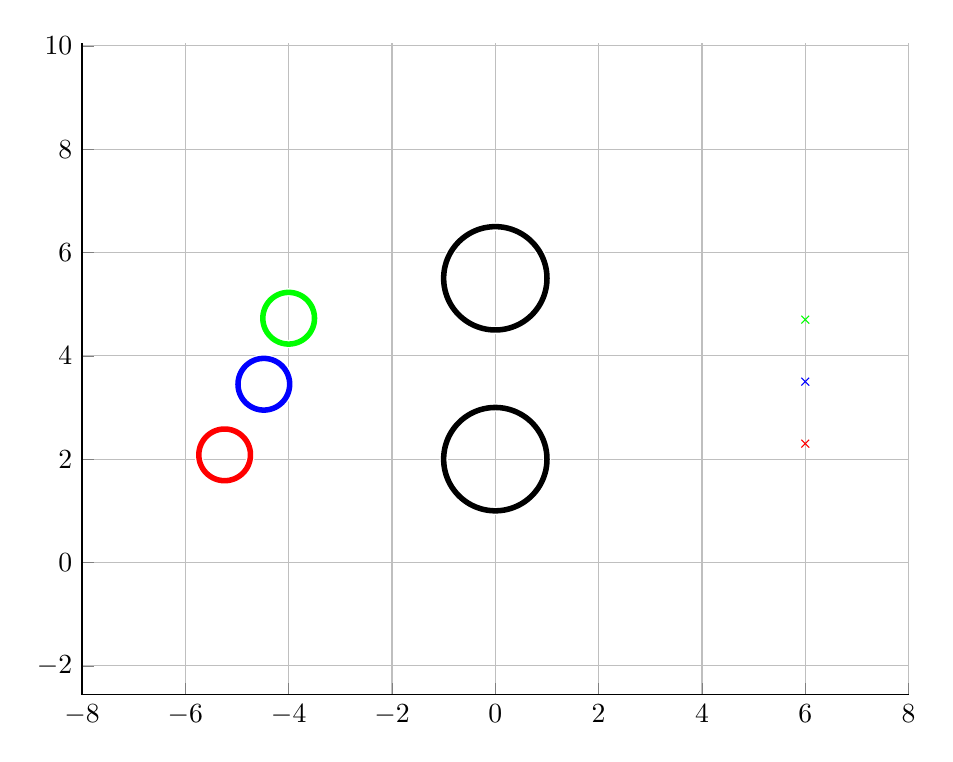
\begin{tikzpicture}

\begin{axis}[%
width=4.133in,
height=3.26in,
at={(0.693in,0.44in)},
scale only axis,
unbounded coords=jump,
xmin=-8,
xmax=8,
xmajorgrids,
ymin=-2.55967741935484,
ymax=10.0596774193548,
ymajorgrids,
axis background/.style={fill=white},
axis x line*=bottom,
axis y line*=left
]
\addplot [color=blue,only marks,mark=x,mark options={solid},forget plot]
  table[row sep=crcr]{%
6	3.5\\
};
\addplot [color=red,only marks,mark=x,mark options={solid},forget plot]
  table[row sep=crcr]{%
6	2.3\\
};
\addplot [color=green,only marks,mark=x,mark options={solid},forget plot]
  table[row sep=crcr]{%
6	4.7\\
};
\addplot [color=white,solid,line width=3.0pt,forget plot]
  table[row sep=crcr]{%
-3.98083876083087	3.44972253450093\\
-3.98114334732132	3.46717228285218\\
-3.98205673570096	3.48460077137299\\
-3.98357781314674	3.50198676613475\\
-3.98570472646009	3.51930908498096\\
-3.98843488432477	3.53654662333439\\
-3.99176496046397	3.55367837990981\\
-3.99569089769287	3.57068348230076\\
-4.00020791286171	3.58754121240943\\
-4.0053105026833	3.6042310316884\\
-4.01099245043792	3.62073260616376\\
-4.01724683354748	3.63702583120888\\
-4.02406603200957	3.65309085603883\\
-4.03144173768129	3.66890810789547\\
-4.03936496440141	3.68445831589387\\
-4.04782605893865	3.69972253450093\\
-4.05681471275266	3.71468216661753\\
-4.06631997455335	3.7293189862363\\
-4.0763302636434	3.74361516064716\\
-4.08683338402751	3.75755327216376\\
-4.09781653927138	3.7711163393442\\
-4.10926634809218	3.78428783768036\\
-4.12116886066155	3.79705171973043\\
-4.13350957560137	3.80939243467025\\
-4.14627345765144	3.82129494723962\\
-4.1594449559876	3.83274475606042\\
-4.17300802316804	3.84372791130429\\
-4.18694613468464	3.8542310316884\\
-4.2012423090955	3.86424132077845\\
-4.21587912871427	3.87374658257914\\
-4.23083876083087	3.88273523639315\\
-4.24610297943793	3.89119633093039\\
-4.26165318743633	3.89911955765051\\
-4.27747043929297	3.90649526332223\\
-4.29353546412292	3.91331446178432\\
-4.30982868916804	3.91956884489388\\
-4.3263302636434	3.9252507926485\\
-4.34302008292237	3.93035338247009\\
-4.35987781303104	3.93487039763893\\
-4.37688291542199	3.93879633486783\\
-4.39401467199741	3.94212641100703\\
-4.41125221035084	3.94485656887171\\
-4.42857452919705	3.94698348218506\\
-4.44596052395881	3.94850455963084\\
-4.46338901247962	3.94941794801048\\
-4.48083876083087	3.94972253450093\\
-4.49828850918212	3.94941794801048\\
-4.51571699770293	3.94850455963084\\
-4.5331029924647	3.94698348218506\\
-4.5504253113109	3.94485656887171\\
-4.56766284966434	3.94212641100703\\
-4.58479460623975	3.93879633486783\\
-4.60179970863071	3.93487039763893\\
-4.61865743873937	3.93035338247009\\
-4.63534725801835	3.9252507926485\\
-4.65184883249371	3.91956884489388\\
-4.66814205753883	3.91331446178432\\
-4.68420708236877	3.90649526332223\\
-4.70002433422541	3.89911955765051\\
-4.71557454222382	3.89119633093039\\
-4.73083876083087	3.88273523639315\\
-4.74579839294748	3.87374658257914\\
-4.76043521256625	3.86424132077845\\
-4.77473138697711	3.8542310316884\\
-4.7886694984937	3.84372791130429\\
-4.80223256567414	3.83274475606042\\
-4.8154040640103	3.82129494723962\\
-4.82816794606037	3.80939243467025\\
-4.8405086610002	3.79705171973043\\
-4.85241117356957	3.78428783768036\\
-4.86386098239036	3.7711163393442\\
-4.87484413763423	3.75755327216376\\
-4.88534725801835	3.74361516064716\\
-4.89535754710839	3.7293189862363\\
-4.90486280890909	3.71468216661753\\
-4.91385146272309	3.69972253450093\\
-4.92231255726034	3.68445831589387\\
-4.93023578398046	3.66890810789547\\
-4.93761148965217	3.65309085603883\\
-4.94443068811427	3.63702583120888\\
-4.95068507122383	3.62073260616376\\
-4.95636701897845	3.6042310316884\\
-4.96146960880003	3.58754121240943\\
-4.96598662396887	3.57068348230076\\
-4.96991256119778	3.55367837990981\\
-4.97324263733698	3.53654662333439\\
-4.97597279520166	3.51930908498096\\
-4.97809970851501	3.50198676613475\\
-4.97962078596078	3.48460077137299\\
-4.98053417434042	3.46717228285218\\
-4.98083876083087	3.44972253450093\\
-4.98053417434042	3.43227278614968\\
-4.97962078596078	3.41484429762887\\
-4.97809970851501	3.3974583028671\\
-4.97597279520166	3.38013598402089\\
-4.97324263733698	3.36289844566746\\
-4.96991256119778	3.34576668909205\\
-4.96598662396887	3.32876158670109\\
-4.96146960880003	3.31190385659243\\
-4.95636701897845	3.29521403731345\\
-4.95068507122383	3.27871246283809\\
-4.94443068811427	3.26241923779297\\
-4.93761148965217	3.24635421296303\\
-4.93023578398046	3.23053696110639\\
-4.92231255726034	3.21498675310798\\
-4.91385146272309	3.19972253450093\\
-4.90486280890909	3.18476290238433\\
-4.89535754710839	3.17012608276555\\
-4.88534725801835	3.15582990835469\\
-4.87484413763423	3.1418917968381\\
-4.86386098239036	3.12832872965766\\
-4.85241117356957	3.1151572313215\\
-4.8405086610002	3.10239334927143\\
-4.82816794606037	3.0900526343316\\
-4.8154040640103	3.07815012176223\\
-4.80223256567414	3.06670031294144\\
-4.7886694984937	3.05571715769757\\
-4.77473138697711	3.04521403731345\\
-4.76043521256625	3.03520374822341\\
-4.74579839294748	3.02569848642271\\
-4.73083876083087	3.01670983260871\\
-4.71557454222382	3.00824873807146\\
-4.70002433422541	3.00032551135134\\
-4.68420708236877	2.99294980567963\\
-4.66814205753883	2.98613060721753\\
-4.65184883249371	2.97987622410797\\
-4.63534725801835	2.97419427635335\\
-4.61865743873937	2.96909168653177\\
-4.60179970863071	2.96457467136293\\
-4.58479460623975	2.96064873413402\\
-4.56766284966434	2.95731865799482\\
-4.5504253113109	2.95458850013014\\
-4.5331029924647	2.95246158681679\\
-4.51571699770293	2.95094050937102\\
-4.49828850918212	2.95002712099138\\
-4.48083876083087	2.94972253450093\\
-4.46338901247962	2.95002712099138\\
-4.44596052395881	2.95094050937102\\
-4.42857452919705	2.95246158681679\\
-4.41125221035084	2.95458850013014\\
-4.39401467199741	2.95731865799482\\
-4.37688291542199	2.96064873413402\\
-4.35987781303104	2.96457467136293\\
-4.34302008292237	2.96909168653177\\
-4.3263302636434	2.97419427635335\\
-4.30982868916804	2.97987622410797\\
-4.29353546412292	2.98613060721753\\
-4.27747043929297	2.99294980567963\\
-4.26165318743633	3.00032551135134\\
-4.24610297943793	3.00824873807146\\
-4.23083876083087	3.01670983260871\\
-4.21587912871427	3.02569848642271\\
-4.2012423090955	3.03520374822341\\
-4.18694613468464	3.04521403731345\\
-4.17300802316804	3.05571715769757\\
-4.1594449559876	3.06670031294144\\
-4.14627345765144	3.07815012176223\\
-4.13350957560137	3.0900526343316\\
-4.12116886066155	3.10239334927143\\
-4.10926634809218	3.1151572313215\\
-4.09781653927138	3.12832872965766\\
-4.08683338402751	3.1418917968381\\
-4.0763302636434	3.15582990835469\\
-4.06631997455335	3.17012608276555\\
-4.05681471275266	3.18476290238432\\
-4.04782605893865	3.19972253450093\\
-4.03936496440141	3.21498675310798\\
-4.03144173768129	3.23053696110639\\
-4.02406603200957	3.24635421296303\\
-4.01724683354748	3.26241923779297\\
-4.01099245043792	3.27871246283809\\
-4.0053105026833	3.29521403731345\\
-4.00020791286171	3.31190385659243\\
-3.99569089769287	3.32876158670109\\
-3.99176496046397	3.34576668909205\\
-3.98843488432477	3.36289844566746\\
-3.98570472646009	3.38013598402089\\
-3.98357781314674	3.3974583028671\\
-3.98205673570096	3.41484429762887\\
-3.98114334732132	3.43227278614968\\
-3.98083876083087	3.44972253450093\\
nan	nan\\
};
\addplot [color=blue,solid,line width=2.0pt,forget plot]
  table[row sep=crcr]{%
-3.98083876083087	3.44972253450093\\
-3.98114334732132	3.46717228285218\\
-3.98205673570096	3.48460077137299\\
-3.98357781314674	3.50198676613475\\
-3.98570472646009	3.51930908498096\\
-3.98843488432477	3.53654662333439\\
-3.99176496046397	3.55367837990981\\
-3.99569089769287	3.57068348230076\\
-4.00020791286171	3.58754121240943\\
-4.0053105026833	3.6042310316884\\
-4.01099245043792	3.62073260616376\\
-4.01724683354748	3.63702583120888\\
-4.02406603200957	3.65309085603883\\
-4.03144173768129	3.66890810789547\\
-4.03936496440141	3.68445831589387\\
-4.04782605893865	3.69972253450093\\
-4.05681471275266	3.71468216661753\\
-4.06631997455335	3.7293189862363\\
-4.0763302636434	3.74361516064716\\
-4.08683338402751	3.75755327216376\\
-4.09781653927138	3.7711163393442\\
-4.10926634809218	3.78428783768036\\
-4.12116886066155	3.79705171973043\\
-4.13350957560137	3.80939243467025\\
-4.14627345765144	3.82129494723962\\
-4.1594449559876	3.83274475606042\\
-4.17300802316804	3.84372791130429\\
-4.18694613468464	3.8542310316884\\
-4.2012423090955	3.86424132077845\\
-4.21587912871427	3.87374658257914\\
-4.23083876083087	3.88273523639315\\
-4.24610297943793	3.89119633093039\\
-4.26165318743633	3.89911955765051\\
-4.27747043929297	3.90649526332223\\
-4.29353546412292	3.91331446178432\\
-4.30982868916804	3.91956884489388\\
-4.3263302636434	3.9252507926485\\
-4.34302008292237	3.93035338247009\\
-4.35987781303104	3.93487039763893\\
-4.37688291542199	3.93879633486783\\
-4.39401467199741	3.94212641100703\\
-4.41125221035084	3.94485656887171\\
-4.42857452919705	3.94698348218506\\
-4.44596052395881	3.94850455963084\\
-4.46338901247962	3.94941794801048\\
-4.48083876083087	3.94972253450093\\
-4.49828850918212	3.94941794801048\\
-4.51571699770293	3.94850455963084\\
-4.5331029924647	3.94698348218506\\
-4.5504253113109	3.94485656887171\\
-4.56766284966434	3.94212641100703\\
-4.58479460623975	3.93879633486783\\
-4.60179970863071	3.93487039763893\\
-4.61865743873937	3.93035338247009\\
-4.63534725801835	3.9252507926485\\
-4.65184883249371	3.91956884489388\\
-4.66814205753883	3.91331446178432\\
-4.68420708236877	3.90649526332223\\
-4.70002433422541	3.89911955765051\\
-4.71557454222382	3.89119633093039\\
-4.73083876083087	3.88273523639315\\
-4.74579839294748	3.87374658257914\\
-4.76043521256625	3.86424132077845\\
-4.77473138697711	3.8542310316884\\
-4.7886694984937	3.84372791130429\\
-4.80223256567414	3.83274475606042\\
-4.8154040640103	3.82129494723962\\
-4.82816794606037	3.80939243467025\\
-4.8405086610002	3.79705171973043\\
-4.85241117356957	3.78428783768036\\
-4.86386098239036	3.7711163393442\\
-4.87484413763423	3.75755327216376\\
-4.88534725801835	3.74361516064716\\
-4.89535754710839	3.7293189862363\\
-4.90486280890909	3.71468216661753\\
-4.91385146272309	3.69972253450093\\
-4.92231255726034	3.68445831589387\\
-4.93023578398046	3.66890810789547\\
-4.93761148965217	3.65309085603883\\
-4.94443068811427	3.63702583120888\\
-4.95068507122383	3.62073260616376\\
-4.95636701897845	3.6042310316884\\
-4.96146960880003	3.58754121240943\\
-4.96598662396887	3.57068348230076\\
-4.96991256119778	3.55367837990981\\
-4.97324263733698	3.53654662333439\\
-4.97597279520166	3.51930908498096\\
-4.97809970851501	3.50198676613475\\
-4.97962078596078	3.48460077137299\\
-4.98053417434042	3.46717228285218\\
-4.98083876083087	3.44972253450093\\
-4.98053417434042	3.43227278614968\\
-4.97962078596078	3.41484429762887\\
-4.97809970851501	3.3974583028671\\
-4.97597279520166	3.38013598402089\\
-4.97324263733698	3.36289844566746\\
-4.96991256119778	3.34576668909205\\
-4.96598662396887	3.32876158670109\\
-4.96146960880003	3.31190385659243\\
-4.95636701897845	3.29521403731345\\
-4.95068507122383	3.27871246283809\\
-4.94443068811427	3.26241923779297\\
-4.93761148965217	3.24635421296303\\
-4.93023578398046	3.23053696110639\\
-4.92231255726034	3.21498675310798\\
-4.91385146272309	3.19972253450093\\
-4.90486280890909	3.18476290238433\\
-4.89535754710839	3.17012608276555\\
-4.88534725801835	3.15582990835469\\
-4.87484413763423	3.1418917968381\\
-4.86386098239036	3.12832872965766\\
-4.85241117356957	3.1151572313215\\
-4.8405086610002	3.10239334927143\\
-4.82816794606037	3.0900526343316\\
-4.8154040640103	3.07815012176223\\
-4.80223256567414	3.06670031294144\\
-4.7886694984937	3.05571715769757\\
-4.77473138697711	3.04521403731345\\
-4.76043521256625	3.03520374822341\\
-4.74579839294748	3.02569848642271\\
-4.73083876083087	3.01670983260871\\
-4.71557454222382	3.00824873807146\\
-4.70002433422541	3.00032551135134\\
-4.68420708236877	2.99294980567963\\
-4.66814205753883	2.98613060721753\\
-4.65184883249371	2.97987622410797\\
-4.63534725801835	2.97419427635335\\
-4.61865743873937	2.96909168653177\\
-4.60179970863071	2.96457467136293\\
-4.58479460623975	2.96064873413402\\
-4.56766284966434	2.95731865799482\\
-4.5504253113109	2.95458850013014\\
-4.5331029924647	2.95246158681679\\
-4.51571699770293	2.95094050937102\\
-4.49828850918212	2.95002712099138\\
-4.48083876083087	2.94972253450093\\
-4.46338901247962	2.95002712099138\\
-4.44596052395881	2.95094050937102\\
-4.42857452919705	2.95246158681679\\
-4.41125221035084	2.95458850013014\\
-4.39401467199741	2.95731865799482\\
-4.37688291542199	2.96064873413402\\
-4.35987781303104	2.96457467136293\\
-4.34302008292237	2.96909168653177\\
-4.3263302636434	2.97419427635335\\
-4.30982868916804	2.97987622410797\\
-4.29353546412292	2.98613060721753\\
-4.27747043929297	2.99294980567963\\
-4.26165318743633	3.00032551135134\\
-4.24610297943793	3.00824873807146\\
-4.23083876083087	3.01670983260871\\
-4.21587912871427	3.02569848642271\\
-4.2012423090955	3.03520374822341\\
-4.18694613468464	3.04521403731345\\
-4.17300802316804	3.05571715769757\\
-4.1594449559876	3.06670031294144\\
-4.14627345765144	3.07815012176223\\
-4.13350957560137	3.0900526343316\\
-4.12116886066155	3.10239334927143\\
-4.10926634809218	3.1151572313215\\
-4.09781653927138	3.12832872965766\\
-4.08683338402751	3.1418917968381\\
-4.0763302636434	3.15582990835469\\
-4.06631997455335	3.17012608276555\\
-4.05681471275266	3.18476290238432\\
-4.04782605893865	3.19972253450093\\
-4.03936496440141	3.21498675310798\\
-4.03144173768129	3.23053696110639\\
-4.02406603200957	3.24635421296303\\
-4.01724683354748	3.26241923779297\\
-4.01099245043792	3.27871246283809\\
-4.0053105026833	3.29521403731345\\
-4.00020791286171	3.31190385659243\\
-3.99569089769287	3.32876158670109\\
-3.99176496046397	3.34576668909205\\
-3.98843488432477	3.36289844566746\\
-3.98570472646009	3.38013598402089\\
-3.98357781314674	3.3974583028671\\
-3.98205673570096	3.41484429762887\\
-3.98114334732132	3.43227278614968\\
-3.98083876083087	3.44972253450093\\
nan	nan\\
};
\addplot [color=white,solid,line width=3.0pt,forget plot]
  table[row sep=crcr]{%
-4.73941569480934	2.08293032320278\\
-4.73972028129979	2.10038007155403\\
-4.74063366967942	2.11780856007484\\
-4.7421547471252	2.13519455483661\\
-4.74428166043855	2.15251687368281\\
-4.74701181830323	2.16975441203625\\
-4.75034189444243	2.18688616861166\\
-4.75426783167134	2.20389127100261\\
-4.75878484684018	2.22074900111128\\
-4.76388743666176	2.23743882039025\\
-4.76956938441638	2.25394039486561\\
-4.77582376752594	2.27023361991074\\
-4.78264296598804	2.28629864474068\\
-4.79001867165975	2.30211589659732\\
-4.79794189837987	2.31766610459573\\
-4.80640299291712	2.33293032320278\\
-4.81539164673112	2.34788995531938\\
-4.82489690853182	2.36252677493815\\
-4.83490719762186	2.37682294934902\\
-4.84541031800598	2.39076106086561\\
-4.85639347324985	2.40432412804605\\
-4.86784328207064	2.41749562638221\\
-4.87974579464001	2.43025950843228\\
-4.89208650957984	2.44260022337211\\
-4.90485039162991	2.45450273594148\\
-4.91802188996607	2.46595254476227\\
-4.93158495714651	2.47693570000614\\
-4.9455230686631	2.48743882039025\\
-4.95981924307396	2.4974491094803\\
-4.97445606269273	2.50695437128099\\
-4.98941569480934	2.515943025095\\
-5.00467991341639	2.52440411963224\\
-5.0202301214148	2.53232734635236\\
-5.03604737327144	2.53970305202408\\
-5.05211239810138	2.54652225048617\\
-5.0684056231465	2.55277663359573\\
-5.08490719762186	2.55845858135036\\
-5.10159701690084	2.56356117117194\\
-5.1184547470095	2.56807818634078\\
-5.13545984940046	2.57200412356968\\
-5.15259160597587	2.57533419970888\\
-5.1698291443293	2.57806435757357\\
-5.18715146317551	2.58019127088692\\
-5.20453745793727	2.58171234833269\\
-5.22196594645809	2.58262573671233\\
-5.23941569480934	2.58293032320278\\
-5.25686544316059	2.58262573671233\\
-5.2742939316814	2.58171234833269\\
-5.29167992644316	2.58019127088692\\
-5.30900224528937	2.57806435757357\\
-5.3262397836428	2.57533419970888\\
-5.34337154021822	2.57200412356968\\
-5.36037664260917	2.56807818634078\\
-5.37723437271784	2.56356117117194\\
-5.39392419199681	2.55845858135036\\
-5.41042576647217	2.55277663359573\\
-5.42671899151729	2.54652225048617\\
-5.44278401634724	2.53970305202408\\
-5.45860126820387	2.53232734635236\\
-5.47415147620228	2.52440411963224\\
-5.48941569480934	2.515943025095\\
-5.50437532692594	2.50695437128099\\
-5.51901214654471	2.4974491094803\\
-5.53330832095557	2.48743882039025\\
-5.54724643247217	2.47693570000614\\
-5.56080949965261	2.46595254476227\\
-5.57398099798877	2.45450273594148\\
-5.58674488003884	2.44260022337211\\
-5.59908559497866	2.43025950843228\\
-5.61098810754803	2.41749562638221\\
-5.62243791636883	2.40432412804605\\
-5.6334210716127	2.39076106086561\\
-5.64392419199681	2.37682294934902\\
-5.65393448108686	2.36252677493815\\
-5.66343974288755	2.34788995531938\\
-5.67242839670156	2.33293032320278\\
-5.6808894912388	2.31766610459573\\
-5.68881271795892	2.30211589659732\\
-5.69618842363064	2.28629864474068\\
-5.70300762209273	2.27023361991074\\
-5.70926200520229	2.25394039486561\\
-5.71494395295691	2.23743882039025\\
-5.7200465427785	2.22074900111128\\
-5.72456355794733	2.20389127100261\\
-5.72848949517624	2.18688616861166\\
-5.73181957131544	2.16975441203625\\
-5.73454972918012	2.15251687368281\\
-5.73667664249347	2.13519455483661\\
-5.73819771993925	2.11780856007484\\
-5.73911110831888	2.10038007155403\\
-5.73941569480934	2.08293032320278\\
-5.73911110831888	2.06548057485153\\
-5.73819771993925	2.04805208633072\\
-5.73667664249347	2.03066609156895\\
-5.73454972918012	2.01334377272275\\
-5.73181957131544	1.99610623436932\\
-5.72848949517624	1.9789744777939\\
-5.72456355794733	1.96196937540295\\
-5.7200465427785	1.94511164529428\\
-5.71494395295691	1.92842182601531\\
-5.70926200520229	1.91192025153995\\
-5.70300762209273	1.89562702649482\\
-5.69618842363064	1.87956200166488\\
-5.68881271795892	1.86374474980824\\
-5.6808894912388	1.84819454180983\\
-5.67242839670156	1.83293032320278\\
-5.66343974288755	1.81797069108618\\
-5.65393448108686	1.80333387146741\\
-5.64392419199681	1.78903769705654\\
-5.6334210716127	1.77509958553995\\
-5.62243791636883	1.76153651835951\\
-5.61098810754803	1.74836502002335\\
-5.59908559497866	1.73560113797328\\
-5.58674488003884	1.72326042303345\\
-5.57398099798877	1.71135791046408\\
-5.56080949965261	1.69990810164329\\
-5.54724643247217	1.68892494639942\\
-5.53330832095557	1.67842182601531\\
-5.51901214654471	1.66841153692526\\
-5.50437532692594	1.65890627512457\\
-5.48941569480934	1.64991762131056\\
-5.47415147620228	1.64145652677332\\
-5.45860126820387	1.6335333000532\\
-5.44278401634724	1.62615759438148\\
-5.42671899151729	1.61933839591939\\
-5.41042576647217	1.61308401280983\\
-5.39392419199681	1.6074020650552\\
-5.37723437271784	1.60229947523362\\
-5.36037664260917	1.59778246006478\\
-5.34337154021822	1.59385652283588\\
-5.3262397836428	1.59052644669668\\
-5.30900224528937	1.587796288832\\
-5.29167992644316	1.58566937551864\\
-5.2742939316814	1.58414829807287\\
-5.25686544316059	1.58323490969323\\
-5.23941569480934	1.58293032320278\\
-5.22196594645809	1.58323490969323\\
-5.20453745793727	1.58414829807287\\
-5.18715146317551	1.58566937551864\\
-5.1698291443293	1.587796288832\\
-5.15259160597587	1.59052644669668\\
-5.13545984940046	1.59385652283588\\
-5.1184547470095	1.59778246006478\\
-5.10159701690084	1.60229947523362\\
-5.08490719762186	1.6074020650552\\
-5.0684056231465	1.61308401280983\\
-5.05211239810138	1.61933839591939\\
-5.03604737327144	1.62615759438148\\
-5.0202301214148	1.6335333000532\\
-5.00467991341639	1.64145652677332\\
-4.98941569480934	1.64991762131056\\
-4.97445606269273	1.65890627512457\\
-4.95981924307396	1.66841153692526\\
-4.9455230686631	1.67842182601531\\
-4.93158495714651	1.68892494639942\\
-4.91802188996607	1.69990810164329\\
-4.90485039162991	1.71135791046408\\
-4.89208650957984	1.72326042303345\\
-4.87974579464001	1.73560113797328\\
-4.86784328207064	1.74836502002335\\
-4.85639347324985	1.76153651835951\\
-4.84541031800598	1.77509958553995\\
-4.83490719762186	1.78903769705654\\
-4.82489690853182	1.80333387146741\\
-4.81539164673112	1.81797069108618\\
-4.80640299291712	1.83293032320278\\
-4.79794189837987	1.84819454180983\\
-4.79001867165975	1.86374474980824\\
-4.78264296598804	1.87956200166488\\
-4.77582376752594	1.89562702649482\\
-4.76956938441638	1.91192025153995\\
-4.76388743666176	1.92842182601531\\
-4.75878484684018	1.94511164529428\\
-4.75426783167134	1.96196937540295\\
-4.75034189444243	1.9789744777939\\
-4.74701181830323	1.99610623436931\\
-4.74428166043855	2.01334377272275\\
-4.7421547471252	2.03066609156895\\
-4.74063366967942	2.04805208633072\\
-4.73972028129979	2.06548057485153\\
-4.73941569480934	2.08293032320278\\
nan	nan\\
};
\addplot [color=red,solid,line width=2.0pt,forget plot]
  table[row sep=crcr]{%
-4.73941569480934	2.08293032320278\\
-4.73972028129979	2.10038007155403\\
-4.74063366967942	2.11780856007484\\
-4.7421547471252	2.13519455483661\\
-4.74428166043855	2.15251687368281\\
-4.74701181830323	2.16975441203625\\
-4.75034189444243	2.18688616861166\\
-4.75426783167134	2.20389127100261\\
-4.75878484684018	2.22074900111128\\
-4.76388743666176	2.23743882039025\\
-4.76956938441638	2.25394039486561\\
-4.77582376752594	2.27023361991074\\
-4.78264296598804	2.28629864474068\\
-4.79001867165975	2.30211589659732\\
-4.79794189837987	2.31766610459573\\
-4.80640299291712	2.33293032320278\\
-4.81539164673112	2.34788995531938\\
-4.82489690853182	2.36252677493815\\
-4.83490719762186	2.37682294934902\\
-4.84541031800598	2.39076106086561\\
-4.85639347324985	2.40432412804605\\
-4.86784328207064	2.41749562638221\\
-4.87974579464001	2.43025950843228\\
-4.89208650957984	2.44260022337211\\
-4.90485039162991	2.45450273594148\\
-4.91802188996607	2.46595254476227\\
-4.93158495714651	2.47693570000614\\
-4.9455230686631	2.48743882039025\\
-4.95981924307396	2.4974491094803\\
-4.97445606269273	2.50695437128099\\
-4.98941569480934	2.515943025095\\
-5.00467991341639	2.52440411963224\\
-5.0202301214148	2.53232734635236\\
-5.03604737327144	2.53970305202408\\
-5.05211239810138	2.54652225048617\\
-5.0684056231465	2.55277663359573\\
-5.08490719762186	2.55845858135036\\
-5.10159701690084	2.56356117117194\\
-5.1184547470095	2.56807818634078\\
-5.13545984940046	2.57200412356968\\
-5.15259160597587	2.57533419970888\\
-5.1698291443293	2.57806435757357\\
-5.18715146317551	2.58019127088692\\
-5.20453745793727	2.58171234833269\\
-5.22196594645809	2.58262573671233\\
-5.23941569480934	2.58293032320278\\
-5.25686544316059	2.58262573671233\\
-5.2742939316814	2.58171234833269\\
-5.29167992644316	2.58019127088692\\
-5.30900224528937	2.57806435757357\\
-5.3262397836428	2.57533419970888\\
-5.34337154021822	2.57200412356968\\
-5.36037664260917	2.56807818634078\\
-5.37723437271784	2.56356117117194\\
-5.39392419199681	2.55845858135036\\
-5.41042576647217	2.55277663359573\\
-5.42671899151729	2.54652225048617\\
-5.44278401634724	2.53970305202408\\
-5.45860126820387	2.53232734635236\\
-5.47415147620228	2.52440411963224\\
-5.48941569480934	2.515943025095\\
-5.50437532692594	2.50695437128099\\
-5.51901214654471	2.4974491094803\\
-5.53330832095557	2.48743882039025\\
-5.54724643247217	2.47693570000614\\
-5.56080949965261	2.46595254476227\\
-5.57398099798877	2.45450273594148\\
-5.58674488003884	2.44260022337211\\
-5.59908559497866	2.43025950843228\\
-5.61098810754803	2.41749562638221\\
-5.62243791636883	2.40432412804605\\
-5.6334210716127	2.39076106086561\\
-5.64392419199681	2.37682294934902\\
-5.65393448108686	2.36252677493815\\
-5.66343974288755	2.34788995531938\\
-5.67242839670156	2.33293032320278\\
-5.6808894912388	2.31766610459573\\
-5.68881271795892	2.30211589659732\\
-5.69618842363064	2.28629864474068\\
-5.70300762209273	2.27023361991074\\
-5.70926200520229	2.25394039486561\\
-5.71494395295691	2.23743882039025\\
-5.7200465427785	2.22074900111128\\
-5.72456355794733	2.20389127100261\\
-5.72848949517624	2.18688616861166\\
-5.73181957131544	2.16975441203625\\
-5.73454972918012	2.15251687368281\\
-5.73667664249347	2.13519455483661\\
-5.73819771993925	2.11780856007484\\
-5.73911110831888	2.10038007155403\\
-5.73941569480934	2.08293032320278\\
-5.73911110831888	2.06548057485153\\
-5.73819771993925	2.04805208633072\\
-5.73667664249347	2.03066609156895\\
-5.73454972918012	2.01334377272275\\
-5.73181957131544	1.99610623436932\\
-5.72848949517624	1.9789744777939\\
-5.72456355794733	1.96196937540295\\
-5.7200465427785	1.94511164529428\\
-5.71494395295691	1.92842182601531\\
-5.70926200520229	1.91192025153995\\
-5.70300762209273	1.89562702649482\\
-5.69618842363064	1.87956200166488\\
-5.68881271795892	1.86374474980824\\
-5.6808894912388	1.84819454180983\\
-5.67242839670156	1.83293032320278\\
-5.66343974288755	1.81797069108618\\
-5.65393448108686	1.80333387146741\\
-5.64392419199681	1.78903769705654\\
-5.6334210716127	1.77509958553995\\
-5.62243791636883	1.76153651835951\\
-5.61098810754803	1.74836502002335\\
-5.59908559497866	1.73560113797328\\
-5.58674488003884	1.72326042303345\\
-5.57398099798877	1.71135791046408\\
-5.56080949965261	1.69990810164329\\
-5.54724643247217	1.68892494639942\\
-5.53330832095557	1.67842182601531\\
-5.51901214654471	1.66841153692526\\
-5.50437532692594	1.65890627512457\\
-5.48941569480934	1.64991762131056\\
-5.47415147620228	1.64145652677332\\
-5.45860126820387	1.6335333000532\\
-5.44278401634724	1.62615759438148\\
-5.42671899151729	1.61933839591939\\
-5.41042576647217	1.61308401280983\\
-5.39392419199681	1.6074020650552\\
-5.37723437271784	1.60229947523362\\
-5.36037664260917	1.59778246006478\\
-5.34337154021822	1.59385652283588\\
-5.3262397836428	1.59052644669668\\
-5.30900224528937	1.587796288832\\
-5.29167992644316	1.58566937551864\\
-5.2742939316814	1.58414829807287\\
-5.25686544316059	1.58323490969323\\
-5.23941569480934	1.58293032320278\\
-5.22196594645809	1.58323490969323\\
-5.20453745793727	1.58414829807287\\
-5.18715146317551	1.58566937551864\\
-5.1698291443293	1.587796288832\\
-5.15259160597587	1.59052644669668\\
-5.13545984940046	1.59385652283588\\
-5.1184547470095	1.59778246006478\\
-5.10159701690084	1.60229947523362\\
-5.08490719762186	1.6074020650552\\
-5.0684056231465	1.61308401280983\\
-5.05211239810138	1.61933839591939\\
-5.03604737327144	1.62615759438148\\
-5.0202301214148	1.6335333000532\\
-5.00467991341639	1.64145652677332\\
-4.98941569480934	1.64991762131056\\
-4.97445606269273	1.65890627512457\\
-4.95981924307396	1.66841153692526\\
-4.9455230686631	1.67842182601531\\
-4.93158495714651	1.68892494639942\\
-4.91802188996607	1.69990810164329\\
-4.90485039162991	1.71135791046408\\
-4.89208650957984	1.72326042303345\\
-4.87974579464001	1.73560113797328\\
-4.86784328207064	1.74836502002335\\
-4.85639347324985	1.76153651835951\\
-4.84541031800598	1.77509958553995\\
-4.83490719762186	1.78903769705654\\
-4.82489690853182	1.80333387146741\\
-4.81539164673112	1.81797069108618\\
-4.80640299291712	1.83293032320278\\
-4.79794189837987	1.84819454180983\\
-4.79001867165975	1.86374474980824\\
-4.78264296598804	1.87956200166488\\
-4.77582376752594	1.89562702649482\\
-4.76956938441638	1.91192025153995\\
-4.76388743666176	1.92842182601531\\
-4.75878484684018	1.94511164529428\\
-4.75426783167134	1.96196937540295\\
-4.75034189444243	1.9789744777939\\
-4.74701181830323	1.99610623436931\\
-4.74428166043855	2.01334377272275\\
-4.7421547471252	2.03066609156895\\
-4.74063366967942	2.04805208633072\\
-4.73972028129979	2.06548057485153\\
-4.73941569480934	2.08293032320278\\
nan	nan\\
};
\addplot [color=white,solid,line width=3.0pt,forget plot]
  table[row sep=crcr]{%
-3.50027573361936	4.72755664336767\\
-3.50058032010981	4.74500639171892\\
-3.50149370848945	4.76243488023973\\
-3.50301478593522	4.7798208750015\\
-3.50514169924857	4.7971431938477\\
-3.50787185711326	4.81438073220114\\
-3.51120193325246	4.83151248877655\\
-3.51512787048136	4.8485175911675\\
-3.5196448856502	4.86537532127617\\
-3.52474747547178	4.88206514055514\\
-3.5304294232264	4.8985667150305\\
-3.53668380633597	4.91485994007563\\
-3.54350300479806	4.93092496490557\\
-3.55087871046978	4.94674221676221\\
-3.5588019371899	4.96229242476062\\
-3.56726303172714	4.97755664336767\\
-3.57625168554115	4.99251627548427\\
-3.58575694734184	5.00715309510304\\
-3.59576723643189	5.02144926951391\\
-3.606270356816	5.0353873810305\\
-3.61725351205987	5.04895044821094\\
-3.62870332088066	5.0621219465471\\
-3.64060583345003	5.07488582859717\\
-3.65294654838986	5.087226543537\\
-3.66571043043993	5.09912905610637\\
-3.67888192877609	5.11057886492716\\
-3.69244499595653	5.12156202017103\\
-3.70638310747312	5.13206514055514\\
-3.72067928188399	5.14207542964519\\
-3.73531610150276	5.15158069144588\\
-3.75027573361936	5.16056934525989\\
-3.76553995222641	5.16903043979713\\
-3.78109016022482	5.17695366651725\\
-3.79690741208146	5.18432937218897\\
-3.8129724369114	5.19114857065106\\
-3.82926566195653	5.19740295376062\\
-3.84576723643189	5.20308490151525\\
-3.86245705571086	5.20818749133683\\
-3.87931478581953	5.21270450650567\\
-3.89631988821048	5.21663044373457\\
-3.91345164478589	5.21996051987377\\
-3.93068918313933	5.22269067773846\\
-3.94801150198553	5.22481759105181\\
-3.9653974967473	5.22633866849758\\
-3.98282598526811	5.22725205687722\\
-4.00027573361936	5.22755664336767\\
-4.01772548197061	5.22725205687722\\
-4.03515397049142	5.22633866849758\\
-4.05253996525319	5.22481759105181\\
-4.06986228409939	5.22269067773846\\
-4.08709982245282	5.21996051987377\\
-4.10423157902824	5.21663044373457\\
-4.12123668141919	5.21270450650567\\
-4.13809441152786	5.20818749133683\\
-4.15478423080683	5.20308490151525\\
-4.17128580528219	5.19740295376062\\
-4.18757903032732	5.19114857065106\\
-4.20364405515726	5.18432937218897\\
-4.2194613070139	5.17695366651725\\
-4.2350115150123	5.16903043979713\\
-4.25027573361936	5.16056934525989\\
-4.26523536573596	5.15158069144588\\
-4.27987218535473	5.14207542964519\\
-4.2941683597656	5.13206514055514\\
-4.30810647128219	5.12156202017103\\
-4.32166953846263	5.11057886492716\\
-4.33484103679879	5.09912905610637\\
-4.34760491884886	5.087226543537\\
-4.35994563378869	5.07488582859717\\
-4.37184814635806	5.0621219465471\\
-4.38329795517885	5.04895044821094\\
-4.39428111042272	5.0353873810305\\
-4.40478423080683	5.02144926951391\\
-4.41479451989688	5.00715309510304\\
-4.42429978169757	4.99251627548427\\
-4.43328843551158	4.97755664336767\\
-4.44174953004882	4.96229242476062\\
-4.44967275676894	4.94674221676221\\
-4.45704846244066	4.93092496490557\\
-4.46386766090275	4.91485994007563\\
-4.47012204401231	4.8985667150305\\
-4.47580399176694	4.88206514055514\\
-4.48090658158852	4.86537532127617\\
-4.48542359675736	4.8485175911675\\
-4.48934953398626	4.83151248877655\\
-4.49267961012546	4.81438073220114\\
-4.49540976799014	4.7971431938477\\
-4.4975366813035	4.7798208750015\\
-4.49905775874927	4.76243488023973\\
-4.49997114712891	4.74500639171892\\
-4.50027573361936	4.72755664336767\\
-4.49997114712891	4.71010689501642\\
-4.49905775874927	4.69267840649561\\
-4.4975366813035	4.67529241173384\\
-4.49540976799014	4.65797009288764\\
-4.49267961012546	4.64073255453421\\
-4.48934953398626	4.62360079795879\\
-4.48542359675736	4.60659569556784\\
-4.48090658158852	4.58973796545917\\
-4.47580399176694	4.5730481461802\\
-4.47012204401231	4.55654657170484\\
-4.46386766090275	4.54025334665971\\
-4.45704846244066	4.52418832182977\\
-4.44967275676894	4.50837106997313\\
-4.44174953004882	4.49282086197472\\
-4.43328843551158	4.47755664336767\\
-4.42429978169757	4.46259701125107\\
-4.41479451989688	4.4479601916323\\
-4.40478423080683	4.43366401722143\\
-4.39428111042272	4.41972590570484\\
-4.38329795517885	4.4061628385244\\
-4.37184814635806	4.39299134018824\\
-4.35994563378869	4.38022745813817\\
-4.34760491884886	4.36788674319835\\
-4.33484103679879	4.35598423062897\\
-4.32166953846263	4.34453442180818\\
-4.30810647128219	4.33355126656431\\
-4.2941683597656	4.3230481461802\\
-4.27987218535473	4.31303785709015\\
-4.26523536573596	4.30353259528946\\
-4.25027573361936	4.29454394147545\\
-4.2350115150123	4.28608284693821\\
-4.2194613070139	4.27815962021809\\
-4.20364405515726	4.27078391454637\\
-4.18757903032732	4.26396471608428\\
-4.17128580528219	4.25771033297472\\
-4.15478423080683	4.25202838522009\\
-4.13809441152786	4.24692579539851\\
-4.12123668141919	4.24240878022967\\
-4.10423157902824	4.23848284300077\\
-4.08709982245282	4.23515276686157\\
-4.06986228409939	4.23242260899688\\
-4.05253996525319	4.23029569568353\\
-4.03515397049142	4.22877461823776\\
-4.01772548197061	4.22786122985812\\
-4.00027573361936	4.22755664336767\\
-3.98282598526811	4.22786122985812\\
-3.9653974967473	4.22877461823776\\
-3.94801150198553	4.23029569568353\\
-3.93068918313933	4.23242260899688\\
-3.91345164478589	4.23515276686157\\
-3.89631988821048	4.23848284300077\\
-3.87931478581953	4.24240878022967\\
-3.86245705571086	4.24692579539851\\
-3.84576723643189	4.25202838522009\\
-3.82926566195653	4.25771033297472\\
-3.8129724369114	4.26396471608428\\
-3.79690741208146	4.27078391454637\\
-3.78109016022482	4.27815962021809\\
-3.76553995222641	4.28608284693821\\
-3.75027573361936	4.29454394147545\\
-3.73531610150276	4.30353259528946\\
-3.72067928188399	4.31303785709015\\
-3.70638310747312	4.3230481461802\\
-3.69244499595653	4.33355126656431\\
-3.67888192877609	4.34453442180818\\
-3.66571043043993	4.35598423062897\\
-3.65294654838986	4.36788674319834\\
-3.64060583345003	4.38022745813817\\
-3.62870332088066	4.39299134018824\\
-3.61725351205987	4.4061628385244\\
-3.606270356816	4.41972590570484\\
-3.59576723643189	4.43366401722143\\
-3.58575694734184	4.4479601916323\\
-3.57625168554115	4.46259701125107\\
-3.56726303172714	4.47755664336767\\
-3.5588019371899	4.49282086197472\\
-3.55087871046978	4.50837106997313\\
-3.54350300479806	4.52418832182977\\
-3.53668380633597	4.54025334665971\\
-3.5304294232264	4.55654657170484\\
-3.52474747547178	4.5730481461802\\
-3.5196448856502	4.58973796545917\\
-3.51512787048136	4.60659569556784\\
-3.51120193325246	4.62360079795879\\
-3.50787185711326	4.6407325545342\\
-3.50514169924857	4.65797009288764\\
-3.50301478593522	4.67529241173384\\
-3.50149370848945	4.69267840649561\\
-3.50058032010981	4.71010689501642\\
-3.50027573361936	4.72755664336767\\
nan	nan\\
};
\addplot [color=green,solid,line width=2.0pt,forget plot]
  table[row sep=crcr]{%
-3.50027573361936	4.72755664336767\\
-3.50058032010981	4.74500639171892\\
-3.50149370848945	4.76243488023973\\
-3.50301478593522	4.7798208750015\\
-3.50514169924857	4.7971431938477\\
-3.50787185711326	4.81438073220114\\
-3.51120193325246	4.83151248877655\\
-3.51512787048136	4.8485175911675\\
-3.5196448856502	4.86537532127617\\
-3.52474747547178	4.88206514055514\\
-3.5304294232264	4.8985667150305\\
-3.53668380633597	4.91485994007563\\
-3.54350300479806	4.93092496490557\\
-3.55087871046978	4.94674221676221\\
-3.5588019371899	4.96229242476062\\
-3.56726303172714	4.97755664336767\\
-3.57625168554115	4.99251627548427\\
-3.58575694734184	5.00715309510304\\
-3.59576723643189	5.02144926951391\\
-3.606270356816	5.0353873810305\\
-3.61725351205987	5.04895044821094\\
-3.62870332088066	5.0621219465471\\
-3.64060583345003	5.07488582859717\\
-3.65294654838986	5.087226543537\\
-3.66571043043993	5.09912905610637\\
-3.67888192877609	5.11057886492716\\
-3.69244499595653	5.12156202017103\\
-3.70638310747312	5.13206514055514\\
-3.72067928188399	5.14207542964519\\
-3.73531610150276	5.15158069144588\\
-3.75027573361936	5.16056934525989\\
-3.76553995222641	5.16903043979713\\
-3.78109016022482	5.17695366651725\\
-3.79690741208146	5.18432937218897\\
-3.8129724369114	5.19114857065106\\
-3.82926566195653	5.19740295376062\\
-3.84576723643189	5.20308490151525\\
-3.86245705571086	5.20818749133683\\
-3.87931478581953	5.21270450650567\\
-3.89631988821048	5.21663044373457\\
-3.91345164478589	5.21996051987377\\
-3.93068918313933	5.22269067773846\\
-3.94801150198553	5.22481759105181\\
-3.9653974967473	5.22633866849758\\
-3.98282598526811	5.22725205687722\\
-4.00027573361936	5.22755664336767\\
-4.01772548197061	5.22725205687722\\
-4.03515397049142	5.22633866849758\\
-4.05253996525319	5.22481759105181\\
-4.06986228409939	5.22269067773846\\
-4.08709982245282	5.21996051987377\\
-4.10423157902824	5.21663044373457\\
-4.12123668141919	5.21270450650567\\
-4.13809441152786	5.20818749133683\\
-4.15478423080683	5.20308490151525\\
-4.17128580528219	5.19740295376062\\
-4.18757903032732	5.19114857065106\\
-4.20364405515726	5.18432937218897\\
-4.2194613070139	5.17695366651725\\
-4.2350115150123	5.16903043979713\\
-4.25027573361936	5.16056934525989\\
-4.26523536573596	5.15158069144588\\
-4.27987218535473	5.14207542964519\\
-4.2941683597656	5.13206514055514\\
-4.30810647128219	5.12156202017103\\
-4.32166953846263	5.11057886492716\\
-4.33484103679879	5.09912905610637\\
-4.34760491884886	5.087226543537\\
-4.35994563378869	5.07488582859717\\
-4.37184814635806	5.0621219465471\\
-4.38329795517885	5.04895044821094\\
-4.39428111042272	5.0353873810305\\
-4.40478423080683	5.02144926951391\\
-4.41479451989688	5.00715309510304\\
-4.42429978169757	4.99251627548427\\
-4.43328843551158	4.97755664336767\\
-4.44174953004882	4.96229242476062\\
-4.44967275676894	4.94674221676221\\
-4.45704846244066	4.93092496490557\\
-4.46386766090275	4.91485994007563\\
-4.47012204401231	4.8985667150305\\
-4.47580399176694	4.88206514055514\\
-4.48090658158852	4.86537532127617\\
-4.48542359675736	4.8485175911675\\
-4.48934953398626	4.83151248877655\\
-4.49267961012546	4.81438073220114\\
-4.49540976799014	4.7971431938477\\
-4.4975366813035	4.7798208750015\\
-4.49905775874927	4.76243488023973\\
-4.49997114712891	4.74500639171892\\
-4.50027573361936	4.72755664336767\\
-4.49997114712891	4.71010689501642\\
-4.49905775874927	4.69267840649561\\
-4.4975366813035	4.67529241173384\\
-4.49540976799014	4.65797009288764\\
-4.49267961012546	4.64073255453421\\
-4.48934953398626	4.62360079795879\\
-4.48542359675736	4.60659569556784\\
-4.48090658158852	4.58973796545917\\
-4.47580399176694	4.5730481461802\\
-4.47012204401231	4.55654657170484\\
-4.46386766090275	4.54025334665971\\
-4.45704846244066	4.52418832182977\\
-4.44967275676894	4.50837106997313\\
-4.44174953004882	4.49282086197472\\
-4.43328843551158	4.47755664336767\\
-4.42429978169757	4.46259701125107\\
-4.41479451989688	4.4479601916323\\
-4.40478423080683	4.43366401722143\\
-4.39428111042272	4.41972590570484\\
-4.38329795517885	4.4061628385244\\
-4.37184814635806	4.39299134018824\\
-4.35994563378869	4.38022745813817\\
-4.34760491884886	4.36788674319835\\
-4.33484103679879	4.35598423062897\\
-4.32166953846263	4.34453442180818\\
-4.30810647128219	4.33355126656431\\
-4.2941683597656	4.3230481461802\\
-4.27987218535473	4.31303785709015\\
-4.26523536573596	4.30353259528946\\
-4.25027573361936	4.29454394147545\\
-4.2350115150123	4.28608284693821\\
-4.2194613070139	4.27815962021809\\
-4.20364405515726	4.27078391454637\\
-4.18757903032732	4.26396471608428\\
-4.17128580528219	4.25771033297472\\
-4.15478423080683	4.25202838522009\\
-4.13809441152786	4.24692579539851\\
-4.12123668141919	4.24240878022967\\
-4.10423157902824	4.23848284300077\\
-4.08709982245282	4.23515276686157\\
-4.06986228409939	4.23242260899688\\
-4.05253996525319	4.23029569568353\\
-4.03515397049142	4.22877461823776\\
-4.01772548197061	4.22786122985812\\
-4.00027573361936	4.22755664336767\\
-3.98282598526811	4.22786122985812\\
-3.9653974967473	4.22877461823776\\
-3.94801150198553	4.23029569568353\\
-3.93068918313933	4.23242260899688\\
-3.91345164478589	4.23515276686157\\
-3.89631988821048	4.23848284300077\\
-3.87931478581953	4.24240878022967\\
-3.86245705571086	4.24692579539851\\
-3.84576723643189	4.25202838522009\\
-3.82926566195653	4.25771033297472\\
-3.8129724369114	4.26396471608428\\
-3.79690741208146	4.27078391454637\\
-3.78109016022482	4.27815962021809\\
-3.76553995222641	4.28608284693821\\
-3.75027573361936	4.29454394147545\\
-3.73531610150276	4.30353259528946\\
-3.72067928188399	4.31303785709015\\
-3.70638310747312	4.3230481461802\\
-3.69244499595653	4.33355126656431\\
-3.67888192877609	4.34453442180818\\
-3.66571043043993	4.35598423062897\\
-3.65294654838986	4.36788674319834\\
-3.64060583345003	4.38022745813817\\
-3.62870332088066	4.39299134018824\\
-3.61725351205987	4.4061628385244\\
-3.606270356816	4.41972590570484\\
-3.59576723643189	4.43366401722143\\
-3.58575694734184	4.4479601916323\\
-3.57625168554115	4.46259701125107\\
-3.56726303172714	4.47755664336767\\
-3.5588019371899	4.49282086197472\\
-3.55087871046978	4.50837106997313\\
-3.54350300479806	4.52418832182977\\
-3.53668380633597	4.54025334665971\\
-3.5304294232264	4.55654657170484\\
-3.52474747547178	4.5730481461802\\
-3.5196448856502	4.58973796545917\\
-3.51512787048136	4.60659569556784\\
-3.51120193325246	4.62360079795879\\
-3.50787185711326	4.6407325545342\\
-3.50514169924857	4.65797009288764\\
-3.50301478593522	4.67529241173384\\
-3.50149370848945	4.69267840649561\\
-3.50058032010981	4.71010689501642\\
-3.50027573361936	4.72755664336767\\
nan	nan\\
};
\addplot [color=white,solid,line width=3.0pt,forget plot]
  table[row sep=crcr]{%
1	2\\
0.999390827019096	2.0348994967025\\
0.997564050259824	2.06975647374413\\
0.994521895368273	2.10452846326765\\
0.99026806874157	2.13917310096007\\
0.984807753012208	2.17364817766693\\
0.978147600733806	2.20791169081776\\
0.970295726275996	2.24192189559967\\
0.961261695938319	2.275637355817\\
0.951056516295154	2.30901699437495\\
0.939692620785908	2.34202014332567\\
0.927183854566787	2.37460659341591\\
0.913545457642601	2.4067366430758\\
0.898794046299167	2.43837114678908\\
0.882947592858927	2.46947156278589\\
0.866025403784439	2.5\\
0.848048096156426	2.5299192642332\\
0.829037572555042	2.55919290347075\\
0.809016994374947	2.58778525229247\\
0.788010753606722	2.61566147532566\\
0.766044443118978	2.64278760968654\\
0.743144825477394	2.66913060635886\\
0.719339800338651	2.694658370459\\
0.694658370458997	2.71933980033865\\
0.669130606358858	2.74314482547739\\
0.642787609686539	2.76604444311898\\
0.615661475325658	2.78801075360672\\
0.587785252292473	2.80901699437495\\
0.559192903470747	2.82903757255504\\
0.529919264233205	2.84804809615643\\
0.5	2.86602540378444\\
0.469471562785891	2.88294759285893\\
0.438371146789077	2.89879404629917\\
0.4067366430758	2.9135454576426\\
0.374606593415912	2.92718385456679\\
0.342020143325669	2.93969262078591\\
0.309016994374947	2.95105651629515\\
0.275637355816999	2.96126169593832\\
0.241921895599668	2.970295726276\\
0.207911690817759	2.97814760073381\\
0.17364817766693	2.98480775301221\\
0.139173100960066	2.99026806874157\\
0.104528463267653	2.99452189536827\\
0.0697564737441255	2.99756405025982\\
0.0348994967025011	2.9993908270191\\
6.12323399573677e-17	3\\
-0.0348994967025007	2.9993908270191\\
-0.0697564737441253	2.99756405025982\\
-0.104528463267653	2.99452189536827\\
-0.139173100960065	2.99026806874157\\
-0.17364817766693	2.98480775301221\\
-0.207911690817759	2.97814760073381\\
-0.241921895599668	2.970295726276\\
-0.275637355816999	2.96126169593832\\
-0.309016994374947	2.95105651629515\\
-0.342020143325669	2.93969262078591\\
-0.374606593415912	2.92718385456679\\
-0.4067366430758	2.9135454576426\\
-0.438371146789078	2.89879404629917\\
-0.469471562785891	2.88294759285893\\
-0.5	2.86602540378444\\
-0.529919264233205	2.84804809615643\\
-0.559192903470747	2.82903757255504\\
-0.587785252292473	2.80901699437495\\
-0.615661475325658	2.78801075360672\\
-0.642787609686539	2.76604444311898\\
-0.669130606358858	2.74314482547739\\
-0.694658370458997	2.71933980033865\\
-0.719339800338651	2.694658370459\\
-0.743144825477394	2.66913060635886\\
-0.766044443118978	2.64278760968654\\
-0.788010753606722	2.61566147532566\\
-0.809016994374947	2.58778525229247\\
-0.829037572555042	2.55919290347075\\
-0.848048096156426	2.5299192642332\\
-0.866025403784439	2.5\\
-0.882947592858927	2.46947156278589\\
-0.898794046299167	2.43837114678908\\
-0.913545457642601	2.4067366430758\\
-0.927183854566787	2.37460659341591\\
-0.939692620785908	2.34202014332567\\
-0.951056516295154	2.30901699437495\\
-0.961261695938319	2.275637355817\\
-0.970295726275996	2.24192189559967\\
-0.978147600733806	2.20791169081776\\
-0.984807753012208	2.17364817766693\\
-0.99026806874157	2.13917310096007\\
-0.994521895368273	2.10452846326765\\
-0.997564050259824	2.06975647374413\\
-0.999390827019096	2.0348994967025\\
-1	2\\
-0.999390827019096	1.9651005032975\\
-0.997564050259824	1.93024352625588\\
-0.994521895368273	1.89547153673235\\
-0.99026806874157	1.86082689903993\\
-0.984807753012208	1.82635182233307\\
-0.978147600733806	1.79208830918224\\
-0.970295726275997	1.75807810440033\\
-0.961261695938319	1.724362644183\\
-0.951056516295154	1.69098300562505\\
-0.939692620785908	1.65797985667433\\
-0.927183854566787	1.62539340658409\\
-0.913545457642601	1.5932633569242\\
-0.898794046299167	1.56162885321092\\
-0.882947592858927	1.53052843721411\\
-0.866025403784439	1.5\\
-0.848048096156426	1.4700807357668\\
-0.829037572555042	1.44080709652925\\
-0.809016994374947	1.41221474770753\\
-0.788010753606722	1.38433852467434\\
-0.766044443118978	1.35721239031346\\
-0.743144825477394	1.33086939364114\\
-0.719339800338651	1.305341629541\\
-0.694658370458997	1.28066019966135\\
-0.669130606358858	1.25685517452261\\
-0.642787609686539	1.23395555688102\\
-0.615661475325658	1.21198924639328\\
-0.587785252292473	1.19098300562505\\
-0.559192903470747	1.17096242744496\\
-0.529919264233205	1.15195190384357\\
-0.5	1.13397459621556\\
-0.469471562785891	1.11705240714107\\
-0.438371146789078	1.10120595370083\\
-0.4067366430758	1.0864545423574\\
-0.374606593415912	1.07281614543321\\
-0.342020143325669	1.06030737921409\\
-0.309016994374948	1.04894348370485\\
-0.275637355816999	1.03873830406168\\
-0.241921895599668	1.029704273724\\
-0.20791169081776	1.02185239926619\\
-0.17364817766693	1.01519224698779\\
-0.139173100960065	1.00973193125843\\
-0.104528463267653	1.00547810463173\\
-0.0697564737441256	1.00243594974018\\
-0.0348994967025016	1.0006091729809\\
-1.83697019872103e-16	1\\
0.0348994967025013	1.0006091729809\\
0.0697564737441252	1.00243594974018\\
0.104528463267653	1.00547810463173\\
0.139173100960065	1.00973193125843\\
0.17364817766693	1.01519224698779\\
0.207911690817759	1.02185239926619\\
0.241921895599667	1.029704273724\\
0.275637355816999	1.03873830406168\\
0.309016994374947	1.04894348370485\\
0.342020143325668	1.06030737921409\\
0.374606593415912	1.07281614543321\\
0.406736643075801	1.0864545423574\\
0.438371146789077	1.10120595370083\\
0.46947156278589	1.11705240714107\\
0.5	1.13397459621556\\
0.529919264233205	1.15195190384357\\
0.559192903470746	1.17096242744496\\
0.587785252292473	1.19098300562505\\
0.615661475325659	1.21198924639328\\
0.642787609686539	1.23395555688102\\
0.669130606358858	1.25685517452261\\
0.694658370458997	1.28066019966135\\
0.719339800338651	1.305341629541\\
0.743144825477394	1.33086939364114\\
0.766044443118978	1.35721239031346\\
0.788010753606722	1.38433852467434\\
0.809016994374947	1.41221474770753\\
0.829037572555041	1.44080709652925\\
0.848048096156425	1.47008073576679\\
0.866025403784438	1.5\\
0.882947592858927	1.53052843721411\\
0.898794046299167	1.56162885321092\\
0.913545457642601	1.5932633569242\\
0.927183854566787	1.62539340658409\\
0.939692620785908	1.65797985667433\\
0.951056516295154	1.69098300562505\\
0.961261695938319	1.724362644183\\
0.970295726275996	1.75807810440033\\
0.978147600733806	1.79208830918224\\
0.984807753012208	1.82635182233307\\
0.99026806874157	1.86082689903993\\
0.994521895368273	1.89547153673235\\
0.997564050259824	1.93024352625588\\
0.999390827019096	1.9651005032975\\
1	2\\
nan	nan\\
};
\addplot [color=black,solid,line width=2.0pt,forget plot]
  table[row sep=crcr]{%
1	2\\
0.999390827019096	2.0348994967025\\
0.997564050259824	2.06975647374413\\
0.994521895368273	2.10452846326765\\
0.99026806874157	2.13917310096007\\
0.984807753012208	2.17364817766693\\
0.978147600733806	2.20791169081776\\
0.970295726275996	2.24192189559967\\
0.961261695938319	2.275637355817\\
0.951056516295154	2.30901699437495\\
0.939692620785908	2.34202014332567\\
0.927183854566787	2.37460659341591\\
0.913545457642601	2.4067366430758\\
0.898794046299167	2.43837114678908\\
0.882947592858927	2.46947156278589\\
0.866025403784439	2.5\\
0.848048096156426	2.5299192642332\\
0.829037572555042	2.55919290347075\\
0.809016994374947	2.58778525229247\\
0.788010753606722	2.61566147532566\\
0.766044443118978	2.64278760968654\\
0.743144825477394	2.66913060635886\\
0.719339800338651	2.694658370459\\
0.694658370458997	2.71933980033865\\
0.669130606358858	2.74314482547739\\
0.642787609686539	2.76604444311898\\
0.615661475325658	2.78801075360672\\
0.587785252292473	2.80901699437495\\
0.559192903470747	2.82903757255504\\
0.529919264233205	2.84804809615643\\
0.5	2.86602540378444\\
0.469471562785891	2.88294759285893\\
0.438371146789077	2.89879404629917\\
0.4067366430758	2.9135454576426\\
0.374606593415912	2.92718385456679\\
0.342020143325669	2.93969262078591\\
0.309016994374947	2.95105651629515\\
0.275637355816999	2.96126169593832\\
0.241921895599668	2.970295726276\\
0.207911690817759	2.97814760073381\\
0.17364817766693	2.98480775301221\\
0.139173100960066	2.99026806874157\\
0.104528463267653	2.99452189536827\\
0.0697564737441255	2.99756405025982\\
0.0348994967025011	2.9993908270191\\
6.12323399573677e-17	3\\
-0.0348994967025007	2.9993908270191\\
-0.0697564737441253	2.99756405025982\\
-0.104528463267653	2.99452189536827\\
-0.139173100960065	2.99026806874157\\
-0.17364817766693	2.98480775301221\\
-0.207911690817759	2.97814760073381\\
-0.241921895599668	2.970295726276\\
-0.275637355816999	2.96126169593832\\
-0.309016994374947	2.95105651629515\\
-0.342020143325669	2.93969262078591\\
-0.374606593415912	2.92718385456679\\
-0.4067366430758	2.9135454576426\\
-0.438371146789078	2.89879404629917\\
-0.469471562785891	2.88294759285893\\
-0.5	2.86602540378444\\
-0.529919264233205	2.84804809615643\\
-0.559192903470747	2.82903757255504\\
-0.587785252292473	2.80901699437495\\
-0.615661475325658	2.78801075360672\\
-0.642787609686539	2.76604444311898\\
-0.669130606358858	2.74314482547739\\
-0.694658370458997	2.71933980033865\\
-0.719339800338651	2.694658370459\\
-0.743144825477394	2.66913060635886\\
-0.766044443118978	2.64278760968654\\
-0.788010753606722	2.61566147532566\\
-0.809016994374947	2.58778525229247\\
-0.829037572555042	2.55919290347075\\
-0.848048096156426	2.5299192642332\\
-0.866025403784439	2.5\\
-0.882947592858927	2.46947156278589\\
-0.898794046299167	2.43837114678908\\
-0.913545457642601	2.4067366430758\\
-0.927183854566787	2.37460659341591\\
-0.939692620785908	2.34202014332567\\
-0.951056516295154	2.30901699437495\\
-0.961261695938319	2.275637355817\\
-0.970295726275996	2.24192189559967\\
-0.978147600733806	2.20791169081776\\
-0.984807753012208	2.17364817766693\\
-0.99026806874157	2.13917310096007\\
-0.994521895368273	2.10452846326765\\
-0.997564050259824	2.06975647374413\\
-0.999390827019096	2.0348994967025\\
-1	2\\
-0.999390827019096	1.9651005032975\\
-0.997564050259824	1.93024352625588\\
-0.994521895368273	1.89547153673235\\
-0.99026806874157	1.86082689903993\\
-0.984807753012208	1.82635182233307\\
-0.978147600733806	1.79208830918224\\
-0.970295726275997	1.75807810440033\\
-0.961261695938319	1.724362644183\\
-0.951056516295154	1.69098300562505\\
-0.939692620785908	1.65797985667433\\
-0.927183854566787	1.62539340658409\\
-0.913545457642601	1.5932633569242\\
-0.898794046299167	1.56162885321092\\
-0.882947592858927	1.53052843721411\\
-0.866025403784439	1.5\\
-0.848048096156426	1.4700807357668\\
-0.829037572555042	1.44080709652925\\
-0.809016994374947	1.41221474770753\\
-0.788010753606722	1.38433852467434\\
-0.766044443118978	1.35721239031346\\
-0.743144825477394	1.33086939364114\\
-0.719339800338651	1.305341629541\\
-0.694658370458997	1.28066019966135\\
-0.669130606358858	1.25685517452261\\
-0.642787609686539	1.23395555688102\\
-0.615661475325658	1.21198924639328\\
-0.587785252292473	1.19098300562505\\
-0.559192903470747	1.17096242744496\\
-0.529919264233205	1.15195190384357\\
-0.5	1.13397459621556\\
-0.469471562785891	1.11705240714107\\
-0.438371146789078	1.10120595370083\\
-0.4067366430758	1.0864545423574\\
-0.374606593415912	1.07281614543321\\
-0.342020143325669	1.06030737921409\\
-0.309016994374948	1.04894348370485\\
-0.275637355816999	1.03873830406168\\
-0.241921895599668	1.029704273724\\
-0.20791169081776	1.02185239926619\\
-0.17364817766693	1.01519224698779\\
-0.139173100960065	1.00973193125843\\
-0.104528463267653	1.00547810463173\\
-0.0697564737441256	1.00243594974018\\
-0.0348994967025016	1.0006091729809\\
-1.83697019872103e-16	1\\
0.0348994967025013	1.0006091729809\\
0.0697564737441252	1.00243594974018\\
0.104528463267653	1.00547810463173\\
0.139173100960065	1.00973193125843\\
0.17364817766693	1.01519224698779\\
0.207911690817759	1.02185239926619\\
0.241921895599667	1.029704273724\\
0.275637355816999	1.03873830406168\\
0.309016994374947	1.04894348370485\\
0.342020143325668	1.06030737921409\\
0.374606593415912	1.07281614543321\\
0.406736643075801	1.0864545423574\\
0.438371146789077	1.10120595370083\\
0.46947156278589	1.11705240714107\\
0.5	1.13397459621556\\
0.529919264233205	1.15195190384357\\
0.559192903470746	1.17096242744496\\
0.587785252292473	1.19098300562505\\
0.615661475325659	1.21198924639328\\
0.642787609686539	1.23395555688102\\
0.669130606358858	1.25685517452261\\
0.694658370458997	1.28066019966135\\
0.719339800338651	1.305341629541\\
0.743144825477394	1.33086939364114\\
0.766044443118978	1.35721239031346\\
0.788010753606722	1.38433852467434\\
0.809016994374947	1.41221474770753\\
0.829037572555041	1.44080709652925\\
0.848048096156425	1.47008073576679\\
0.866025403784438	1.5\\
0.882947592858927	1.53052843721411\\
0.898794046299167	1.56162885321092\\
0.913545457642601	1.5932633569242\\
0.927183854566787	1.62539340658409\\
0.939692620785908	1.65797985667433\\
0.951056516295154	1.69098300562505\\
0.961261695938319	1.724362644183\\
0.970295726275996	1.75807810440033\\
0.978147600733806	1.79208830918224\\
0.984807753012208	1.82635182233307\\
0.99026806874157	1.86082689903993\\
0.994521895368273	1.89547153673235\\
0.997564050259824	1.93024352625588\\
0.999390827019096	1.9651005032975\\
1	2\\
nan	nan\\
};
\addplot [color=white,solid,line width=3.0pt,forget plot]
  table[row sep=crcr]{%
1	5.5\\
0.999390827019096	5.5348994967025\\
0.997564050259824	5.56975647374413\\
0.994521895368273	5.60452846326765\\
0.99026806874157	5.63917310096007\\
0.984807753012208	5.67364817766693\\
0.978147600733806	5.70791169081776\\
0.970295726275996	5.74192189559967\\
0.961261695938319	5.775637355817\\
0.951056516295154	5.80901699437495\\
0.939692620785908	5.84202014332567\\
0.927183854566787	5.87460659341591\\
0.913545457642601	5.9067366430758\\
0.898794046299167	5.93837114678908\\
0.882947592858927	5.96947156278589\\
0.866025403784439	6\\
0.848048096156426	6.0299192642332\\
0.829037572555042	6.05919290347075\\
0.809016994374947	6.08778525229247\\
0.788010753606722	6.11566147532566\\
0.766044443118978	6.14278760968654\\
0.743144825477394	6.16913060635886\\
0.719339800338651	6.194658370459\\
0.694658370458997	6.21933980033865\\
0.669130606358858	6.24314482547739\\
0.642787609686539	6.26604444311898\\
0.615661475325658	6.28801075360672\\
0.587785252292473	6.30901699437495\\
0.559192903470747	6.32903757255504\\
0.529919264233205	6.34804809615643\\
0.5	6.36602540378444\\
0.469471562785891	6.38294759285893\\
0.438371146789077	6.39879404629917\\
0.4067366430758	6.4135454576426\\
0.374606593415912	6.42718385456679\\
0.342020143325669	6.43969262078591\\
0.309016994374947	6.45105651629515\\
0.275637355816999	6.46126169593832\\
0.241921895599668	6.470295726276\\
0.207911690817759	6.47814760073381\\
0.17364817766693	6.48480775301221\\
0.139173100960066	6.49026806874157\\
0.104528463267653	6.49452189536827\\
0.0697564737441255	6.49756405025982\\
0.0348994967025011	6.4993908270191\\
6.12323399573677e-17	6.5\\
-0.0348994967025007	6.4993908270191\\
-0.0697564737441253	6.49756405025982\\
-0.104528463267653	6.49452189536827\\
-0.139173100960065	6.49026806874157\\
-0.17364817766693	6.48480775301221\\
-0.207911690817759	6.47814760073381\\
-0.241921895599668	6.470295726276\\
-0.275637355816999	6.46126169593832\\
-0.309016994374947	6.45105651629515\\
-0.342020143325669	6.43969262078591\\
-0.374606593415912	6.42718385456679\\
-0.4067366430758	6.4135454576426\\
-0.438371146789078	6.39879404629917\\
-0.469471562785891	6.38294759285893\\
-0.5	6.36602540378444\\
-0.529919264233205	6.34804809615643\\
-0.559192903470747	6.32903757255504\\
-0.587785252292473	6.30901699437495\\
-0.615661475325658	6.28801075360672\\
-0.642787609686539	6.26604444311898\\
-0.669130606358858	6.24314482547739\\
-0.694658370458997	6.21933980033865\\
-0.719339800338651	6.194658370459\\
-0.743144825477394	6.16913060635886\\
-0.766044443118978	6.14278760968654\\
-0.788010753606722	6.11566147532566\\
-0.809016994374947	6.08778525229247\\
-0.829037572555042	6.05919290347075\\
-0.848048096156426	6.0299192642332\\
-0.866025403784439	6\\
-0.882947592858927	5.96947156278589\\
-0.898794046299167	5.93837114678908\\
-0.913545457642601	5.9067366430758\\
-0.927183854566787	5.87460659341591\\
-0.939692620785908	5.84202014332567\\
-0.951056516295154	5.80901699437495\\
-0.961261695938319	5.775637355817\\
-0.970295726275996	5.74192189559967\\
-0.978147600733806	5.70791169081776\\
-0.984807753012208	5.67364817766693\\
-0.99026806874157	5.63917310096007\\
-0.994521895368273	5.60452846326765\\
-0.997564050259824	5.56975647374413\\
-0.999390827019096	5.5348994967025\\
-1	5.5\\
-0.999390827019096	5.4651005032975\\
-0.997564050259824	5.43024352625588\\
-0.994521895368273	5.39547153673235\\
-0.99026806874157	5.36082689903993\\
-0.984807753012208	5.32635182233307\\
-0.978147600733806	5.29208830918224\\
-0.970295726275997	5.25807810440033\\
-0.961261695938319	5.224362644183\\
-0.951056516295154	5.19098300562505\\
-0.939692620785908	5.15797985667433\\
-0.927183854566787	5.12539340658409\\
-0.913545457642601	5.0932633569242\\
-0.898794046299167	5.06162885321092\\
-0.882947592858927	5.03052843721411\\
-0.866025403784439	5\\
-0.848048096156426	4.9700807357668\\
-0.829037572555042	4.94080709652925\\
-0.809016994374947	4.91221474770753\\
-0.788010753606722	4.88433852467434\\
-0.766044443118978	4.85721239031346\\
-0.743144825477394	4.83086939364114\\
-0.719339800338651	4.805341629541\\
-0.694658370458997	4.78066019966135\\
-0.669130606358858	4.75685517452261\\
-0.642787609686539	4.73395555688102\\
-0.615661475325658	4.71198924639328\\
-0.587785252292473	4.69098300562505\\
-0.559192903470747	4.67096242744496\\
-0.529919264233205	4.65195190384357\\
-0.5	4.63397459621556\\
-0.469471562785891	4.61705240714107\\
-0.438371146789078	4.60120595370083\\
-0.4067366430758	4.5864545423574\\
-0.374606593415912	4.57281614543321\\
-0.342020143325669	4.56030737921409\\
-0.309016994374948	4.54894348370485\\
-0.275637355816999	4.53873830406168\\
-0.241921895599668	4.529704273724\\
-0.20791169081776	4.52185239926619\\
-0.17364817766693	4.51519224698779\\
-0.139173100960065	4.50973193125843\\
-0.104528463267653	4.50547810463173\\
-0.0697564737441256	4.50243594974018\\
-0.0348994967025016	4.5006091729809\\
-1.83697019872103e-16	4.5\\
0.0348994967025013	4.5006091729809\\
0.0697564737441252	4.50243594974018\\
0.104528463267653	4.50547810463173\\
0.139173100960065	4.50973193125843\\
0.17364817766693	4.51519224698779\\
0.207911690817759	4.52185239926619\\
0.241921895599667	4.529704273724\\
0.275637355816999	4.53873830406168\\
0.309016994374947	4.54894348370485\\
0.342020143325668	4.56030737921409\\
0.374606593415912	4.57281614543321\\
0.406736643075801	4.5864545423574\\
0.438371146789077	4.60120595370083\\
0.46947156278589	4.61705240714107\\
0.5	4.63397459621556\\
0.529919264233205	4.65195190384357\\
0.559192903470746	4.67096242744496\\
0.587785252292473	4.69098300562505\\
0.615661475325659	4.71198924639328\\
0.642787609686539	4.73395555688102\\
0.669130606358858	4.75685517452261\\
0.694658370458997	4.78066019966135\\
0.719339800338651	4.805341629541\\
0.743144825477394	4.83086939364114\\
0.766044443118978	4.85721239031346\\
0.788010753606722	4.88433852467434\\
0.809016994374947	4.91221474770753\\
0.829037572555041	4.94080709652925\\
0.848048096156425	4.97008073576679\\
0.866025403784438	5\\
0.882947592858927	5.03052843721411\\
0.898794046299167	5.06162885321092\\
0.913545457642601	5.0932633569242\\
0.927183854566787	5.12539340658409\\
0.939692620785908	5.15797985667433\\
0.951056516295154	5.19098300562505\\
0.961261695938319	5.224362644183\\
0.970295726275996	5.25807810440033\\
0.978147600733806	5.29208830918224\\
0.984807753012208	5.32635182233307\\
0.99026806874157	5.36082689903993\\
0.994521895368273	5.39547153673235\\
0.997564050259824	5.43024352625588\\
0.999390827019096	5.4651005032975\\
1	5.5\\
nan	nan\\
};
\addplot [color=black,solid,line width=2.0pt,forget plot]
  table[row sep=crcr]{%
1	5.5\\
0.999390827019096	5.5348994967025\\
0.997564050259824	5.56975647374413\\
0.994521895368273	5.60452846326765\\
0.99026806874157	5.63917310096007\\
0.984807753012208	5.67364817766693\\
0.978147600733806	5.70791169081776\\
0.970295726275996	5.74192189559967\\
0.961261695938319	5.775637355817\\
0.951056516295154	5.80901699437495\\
0.939692620785908	5.84202014332567\\
0.927183854566787	5.87460659341591\\
0.913545457642601	5.9067366430758\\
0.898794046299167	5.93837114678908\\
0.882947592858927	5.96947156278589\\
0.866025403784439	6\\
0.848048096156426	6.0299192642332\\
0.829037572555042	6.05919290347075\\
0.809016994374947	6.08778525229247\\
0.788010753606722	6.11566147532566\\
0.766044443118978	6.14278760968654\\
0.743144825477394	6.16913060635886\\
0.719339800338651	6.194658370459\\
0.694658370458997	6.21933980033865\\
0.669130606358858	6.24314482547739\\
0.642787609686539	6.26604444311898\\
0.615661475325658	6.28801075360672\\
0.587785252292473	6.30901699437495\\
0.559192903470747	6.32903757255504\\
0.529919264233205	6.34804809615643\\
0.5	6.36602540378444\\
0.469471562785891	6.38294759285893\\
0.438371146789077	6.39879404629917\\
0.4067366430758	6.4135454576426\\
0.374606593415912	6.42718385456679\\
0.342020143325669	6.43969262078591\\
0.309016994374947	6.45105651629515\\
0.275637355816999	6.46126169593832\\
0.241921895599668	6.470295726276\\
0.207911690817759	6.47814760073381\\
0.17364817766693	6.48480775301221\\
0.139173100960066	6.49026806874157\\
0.104528463267653	6.49452189536827\\
0.0697564737441255	6.49756405025982\\
0.0348994967025011	6.4993908270191\\
6.12323399573677e-17	6.5\\
-0.0348994967025007	6.4993908270191\\
-0.0697564737441253	6.49756405025982\\
-0.104528463267653	6.49452189536827\\
-0.139173100960065	6.49026806874157\\
-0.17364817766693	6.48480775301221\\
-0.207911690817759	6.47814760073381\\
-0.241921895599668	6.470295726276\\
-0.275637355816999	6.46126169593832\\
-0.309016994374947	6.45105651629515\\
-0.342020143325669	6.43969262078591\\
-0.374606593415912	6.42718385456679\\
-0.4067366430758	6.4135454576426\\
-0.438371146789078	6.39879404629917\\
-0.469471562785891	6.38294759285893\\
-0.5	6.36602540378444\\
-0.529919264233205	6.34804809615643\\
-0.559192903470747	6.32903757255504\\
-0.587785252292473	6.30901699437495\\
-0.615661475325658	6.28801075360672\\
-0.642787609686539	6.26604444311898\\
-0.669130606358858	6.24314482547739\\
-0.694658370458997	6.21933980033865\\
-0.719339800338651	6.194658370459\\
-0.743144825477394	6.16913060635886\\
-0.766044443118978	6.14278760968654\\
-0.788010753606722	6.11566147532566\\
-0.809016994374947	6.08778525229247\\
-0.829037572555042	6.05919290347075\\
-0.848048096156426	6.0299192642332\\
-0.866025403784439	6\\
-0.882947592858927	5.96947156278589\\
-0.898794046299167	5.93837114678908\\
-0.913545457642601	5.9067366430758\\
-0.927183854566787	5.87460659341591\\
-0.939692620785908	5.84202014332567\\
-0.951056516295154	5.80901699437495\\
-0.961261695938319	5.775637355817\\
-0.970295726275996	5.74192189559967\\
-0.978147600733806	5.70791169081776\\
-0.984807753012208	5.67364817766693\\
-0.99026806874157	5.63917310096007\\
-0.994521895368273	5.60452846326765\\
-0.997564050259824	5.56975647374413\\
-0.999390827019096	5.5348994967025\\
-1	5.5\\
-0.999390827019096	5.4651005032975\\
-0.997564050259824	5.43024352625588\\
-0.994521895368273	5.39547153673235\\
-0.99026806874157	5.36082689903993\\
-0.984807753012208	5.32635182233307\\
-0.978147600733806	5.29208830918224\\
-0.970295726275997	5.25807810440033\\
-0.961261695938319	5.224362644183\\
-0.951056516295154	5.19098300562505\\
-0.939692620785908	5.15797985667433\\
-0.927183854566787	5.12539340658409\\
-0.913545457642601	5.0932633569242\\
-0.898794046299167	5.06162885321092\\
-0.882947592858927	5.03052843721411\\
-0.866025403784439	5\\
-0.848048096156426	4.9700807357668\\
-0.829037572555042	4.94080709652925\\
-0.809016994374947	4.91221474770753\\
-0.788010753606722	4.88433852467434\\
-0.766044443118978	4.85721239031346\\
-0.743144825477394	4.83086939364114\\
-0.719339800338651	4.805341629541\\
-0.694658370458997	4.78066019966135\\
-0.669130606358858	4.75685517452261\\
-0.642787609686539	4.73395555688102\\
-0.615661475325658	4.71198924639328\\
-0.587785252292473	4.69098300562505\\
-0.559192903470747	4.67096242744496\\
-0.529919264233205	4.65195190384357\\
-0.5	4.63397459621556\\
-0.469471562785891	4.61705240714107\\
-0.438371146789078	4.60120595370083\\
-0.4067366430758	4.5864545423574\\
-0.374606593415912	4.57281614543321\\
-0.342020143325669	4.56030737921409\\
-0.309016994374948	4.54894348370485\\
-0.275637355816999	4.53873830406168\\
-0.241921895599668	4.529704273724\\
-0.20791169081776	4.52185239926619\\
-0.17364817766693	4.51519224698779\\
-0.139173100960065	4.50973193125843\\
-0.104528463267653	4.50547810463173\\
-0.0697564737441256	4.50243594974018\\
-0.0348994967025016	4.5006091729809\\
-1.83697019872103e-16	4.5\\
0.0348994967025013	4.5006091729809\\
0.0697564737441252	4.50243594974018\\
0.104528463267653	4.50547810463173\\
0.139173100960065	4.50973193125843\\
0.17364817766693	4.51519224698779\\
0.207911690817759	4.52185239926619\\
0.241921895599667	4.529704273724\\
0.275637355816999	4.53873830406168\\
0.309016994374947	4.54894348370485\\
0.342020143325668	4.56030737921409\\
0.374606593415912	4.57281614543321\\
0.406736643075801	4.5864545423574\\
0.438371146789077	4.60120595370083\\
0.46947156278589	4.61705240714107\\
0.5	4.63397459621556\\
0.529919264233205	4.65195190384357\\
0.559192903470746	4.67096242744496\\
0.587785252292473	4.69098300562505\\
0.615661475325659	4.71198924639328\\
0.642787609686539	4.73395555688102\\
0.669130606358858	4.75685517452261\\
0.694658370458997	4.78066019966135\\
0.719339800338651	4.805341629541\\
0.743144825477394	4.83086939364114\\
0.766044443118978	4.85721239031346\\
0.788010753606722	4.88433852467434\\
0.809016994374947	4.91221474770753\\
0.829037572555041	4.94080709652925\\
0.848048096156425	4.97008073576679\\
0.866025403784438	5\\
0.882947592858927	5.03052843721411\\
0.898794046299167	5.06162885321092\\
0.913545457642601	5.0932633569242\\
0.927183854566787	5.12539340658409\\
0.939692620785908	5.15797985667433\\
0.951056516295154	5.19098300562505\\
0.961261695938319	5.224362644183\\
0.970295726275996	5.25807810440033\\
0.978147600733806	5.29208830918224\\
0.984807753012208	5.32635182233307\\
0.99026806874157	5.36082689903993\\
0.994521895368273	5.39547153673235\\
0.997564050259824	5.43024352625588\\
0.999390827019096	5.4651005032975\\
1	5.5\\
nan	nan\\
};
\end{axis}
\end{tikzpicture}%}
      \caption{}
      \label{}
    \end{figure}
  \end{minipage}
\end{minipage}
}

\noindent\makebox[\linewidth][c]{%
\begin{minipage}{\linewidth}
  \begin{minipage}{0.45\linewidth}
    \begin{figure}[H]
      \scalebox{0.7}{% This file was created by matlab2tikz.
%
%The latest updates can be retrieved from
%  http://www.mathworks.com/matlabcentral/fileexchange/22022-matlab2tikz-matlab2tikz
%where you can also make suggestions and rate matlab2tikz.
%
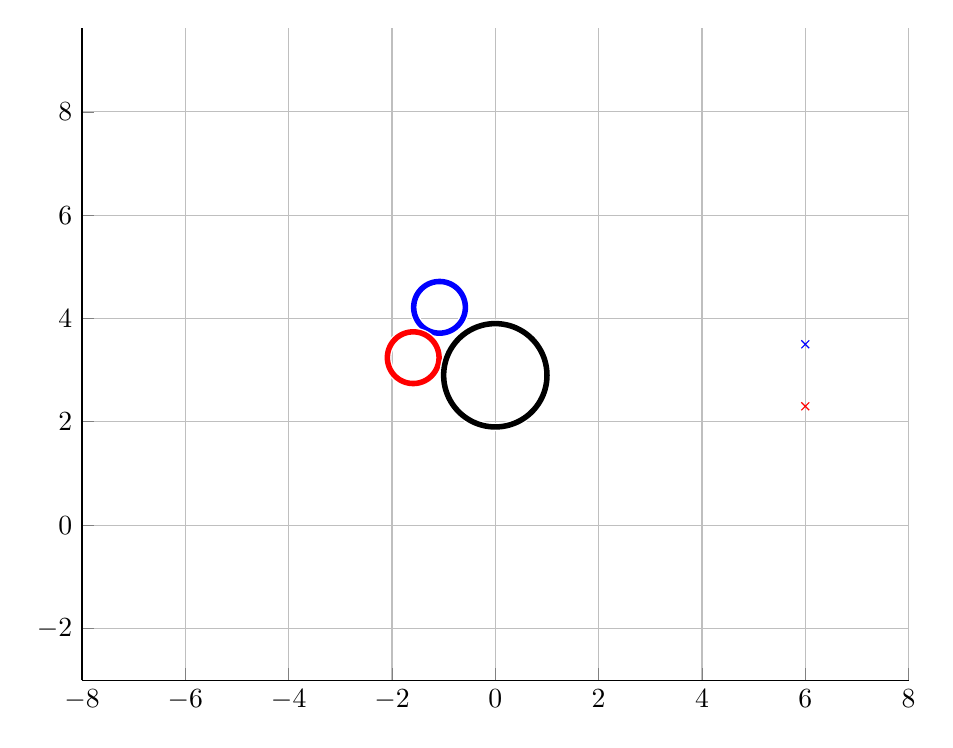
\begin{tikzpicture}

\begin{axis}[%
width=4.133in,
height=3.26in,
at={(0.693in,0.44in)},
scale only axis,
unbounded coords=jump,
xmin=-8,
xmax=8,
xmajorgrids,
ymin=-3.00205312257439,
ymax=9.61730171613528,
ymajorgrids,
axis background/.style={fill=white},
axis x line*=bottom,
axis y line*=left
]
\addplot [color=blue,only marks,mark=x,mark options={solid},forget plot]
  table[row sep=crcr]{%
6	3.5\\
};
\addplot [color=red,only marks,mark=x,mark options={solid},forget plot]
  table[row sep=crcr]{%
6	2.3\\
};
\addplot [color=white,solid,line width=3.0pt,forget plot]
  table[row sep=crcr]{%
-0.580012556236331	4.21524859356089\\
-0.580317142726783	4.23269834191214\\
-0.581230531106419	4.25012683043296\\
-0.582751608552194	4.26751282519472\\
-0.584878521865546	4.28483514404093\\
-0.587608679730227	4.30207268239436\\
-0.590938755869428	4.31920443896977\\
-0.594864693098333	4.33620954136073\\
-0.599381708267171	4.35306727146939\\
-0.604484298088754	4.36975709074837\\
-0.610166245843377	4.38625866522373\\
-0.616420628952937	4.40255189026885\\
-0.62323982741503	4.41861691509879\\
-0.630615533086747	4.43443416695543\\
-0.638538759806867	4.44998437495384\\
-0.646999854344111	4.46524859356089\\
-0.655988508158118	4.4802082256775\\
-0.66549376995881	4.49484504529627\\
-0.675504059048857	4.50914121970713\\
-0.68600717943297	4.52307933122372\\
-0.696990334676842	4.53664239840416\\
-0.708440143497634	4.54981389674032\\
-0.720342656067005	4.56257777879039\\
-0.732683371006832	4.57491849373022\\
-0.745447253056902	4.58682100629959\\
-0.758618751393061	4.59827081512038\\
-0.772181818573502	4.60925397036425\\
-0.786119930090094	4.61975709074837\\
-0.800416104500957	4.62976737983841\\
-0.815052924119728	4.63927264163911\\
-0.830012556236331	4.64826129545311\\
-0.845276774843385	4.65672238999036\\
-0.860826982841792	4.66464561671048\\
-0.876644234698431	4.67202132238219\\
-0.892709259528375	4.67884052084429\\
-0.909002484573496	4.68509490395385\\
-0.925504059048857	4.69077685170847\\
-0.942193878327831	4.69587944153005\\
-0.959051608436497	4.70039645669889\\
-0.976056710827451	4.7043223939278\\
-0.993188467402865	4.707652470067\\
-1.0104260057563	4.71038262793168\\
-1.0277483246025	4.71250954124503\\
-1.04513431936427	4.7140306186908\\
-1.06256280788508	4.71494400707044\\
-1.08001255623633	4.71524859356089\\
-1.09746230458758	4.71494400707044\\
-1.11489079310839	4.7140306186908\\
-1.13227678787016	4.71250954124503\\
-1.14959910671636	4.71038262793168\\
-1.1668366450698	4.707652470067\\
-1.18396840164521	4.7043223939278\\
-1.20097350403616	4.70039645669889\\
-1.21783123414483	4.69587944153005\\
-1.2345210534238	4.69077685170847\\
-1.25102262789917	4.68509490395385\\
-1.26731585294429	4.67884052084429\\
-1.28338087777423	4.67202132238219\\
-1.29919812963087	4.66464561671048\\
-1.31474833762928	4.65672238999036\\
-1.33001255623633	4.64826129545311\\
-1.34497218835293	4.63927264163911\\
-1.3596090079717	4.62976737983841\\
-1.37390518238257	4.61975709074837\\
-1.38784329389916	4.60925397036425\\
-1.4014063610796	4.59827081512038\\
-1.41457785941576	4.58682100629959\\
-1.42734174146583	4.57491849373022\\
-1.43968245640566	4.56257777879039\\
-1.45158496897503	4.54981389674032\\
-1.46303477779582	4.53664239840416\\
-1.47401793303969	4.52307933122372\\
-1.4845210534238	4.50914121970713\\
-1.49453134251385	4.49484504529627\\
-1.50403660431454	4.4802082256775\\
-1.51302525812855	4.46524859356089\\
-1.52148635266579	4.44998437495384\\
-1.52940957938591	4.43443416695543\\
-1.53678528505763	4.41861691509879\\
-1.54360448351972	4.40255189026885\\
-1.54985886662928	4.38625866522373\\
-1.55554081438391	4.36975709074837\\
-1.56064340420549	4.35306727146939\\
-1.56516041937433	4.33620954136073\\
-1.56908635660323	4.31920443896977\\
-1.57241643274243	4.30207268239436\\
-1.57514659060712	4.28483514404093\\
-1.57727350392047	4.26751282519472\\
-1.57879458136624	4.25012683043296\\
-1.57970796974588	4.23269834191214\\
-1.58001255623633	4.21524859356089\\
-1.57970796974588	4.19779884520964\\
-1.57879458136624	4.18037035668883\\
-1.57727350392047	4.16298436192707\\
-1.57514659060712	4.14566204308086\\
-1.57241643274243	4.12842450472743\\
-1.56908635660323	4.11129274815201\\
-1.56516041937433	4.09428764576106\\
-1.56064340420549	4.07742991565239\\
-1.55554081438391	4.06074009637342\\
-1.54985886662928	4.04423852189806\\
-1.54360448351972	4.02794529685294\\
-1.53678528505763	4.01188027202299\\
-1.52940957938591	3.99606302016635\\
-1.52148635266579	3.98051281216795\\
-1.51302525812855	3.96524859356089\\
-1.50403660431454	3.95028896144429\\
-1.49453134251385	3.93565214182552\\
-1.4845210534238	3.92135596741466\\
-1.47401793303969	3.90741785589806\\
-1.46303477779582	3.89385478871762\\
-1.45158496897503	3.88068329038146\\
-1.43968245640566	3.86791940833139\\
-1.42734174146583	3.85557869339157\\
-1.41457785941576	3.8436761808222\\
-1.4014063610796	3.8322263720014\\
-1.38784329389916	3.82124321675753\\
-1.37390518238257	3.81074009637342\\
-1.3596090079717	3.80072980728337\\
-1.34497218835293	3.79122454548268\\
-1.33001255623633	3.78223589166867\\
-1.31474833762928	3.77377479713143\\
-1.29919812963087	3.76585157041131\\
-1.28338087777423	3.75847586473959\\
-1.26731585294429	3.7516566662775\\
-1.25102262789917	3.74540228316794\\
-1.2345210534238	3.73972033541332\\
-1.21783123414483	3.73461774559173\\
-1.20097350403616	3.73010073042289\\
-1.18396840164521	3.72617479319399\\
-1.1668366450698	3.72284471705479\\
-1.14959910671636	3.72011455919011\\
-1.13227678787016	3.71798764587676\\
-1.11489079310839	3.71646656843098\\
-1.09746230458758	3.71555318005134\\
-1.08001255623633	3.71524859356089\\
-1.06256280788508	3.71555318005134\\
-1.04513431936427	3.71646656843098\\
-1.0277483246025	3.71798764587676\\
-1.0104260057563	3.72011455919011\\
-0.993188467402866	3.72284471705479\\
-0.976056710827451	3.72617479319399\\
-0.959051608436497	3.73010073042289\\
-0.942193878327831	3.73461774559173\\
-0.925504059048857	3.73972033541332\\
-0.909002484573497	3.74540228316794\\
-0.892709259528375	3.7516566662775\\
-0.87664423469843	3.75847586473959\\
-0.860826982841792	3.76585157041131\\
-0.845276774843386	3.77377479713143\\
-0.830012556236331	3.78223589166867\\
-0.815052924119728	3.79122454548268\\
-0.800416104500958	3.80072980728337\\
-0.786119930090094	3.81074009637342\\
-0.772181818573501	3.82124321675753\\
-0.758618751393061	3.8322263720014\\
-0.745447253056902	3.8436761808222\\
-0.732683371006832	3.85557869339157\\
-0.720342656067005	3.86791940833139\\
-0.708440143497634	3.88068329038146\\
-0.696990334676842	3.89385478871762\\
-0.68600717943297	3.90741785589806\\
-0.675504059048857	3.92135596741466\\
-0.66549376995881	3.93565214182552\\
-0.655988508158118	3.95028896144429\\
-0.646999854344112	3.96524859356089\\
-0.638538759806867	3.98051281216795\\
-0.630615533086747	3.99606302016635\\
-0.62323982741503	4.01188027202299\\
-0.616420628952937	4.02794529685294\\
-0.610166245843377	4.04423852189806\\
-0.604484298088754	4.06074009637342\\
-0.599381708267171	4.07742991565239\\
-0.594864693098333	4.09428764576106\\
-0.590938755869428	4.11129274815201\\
-0.587608679730227	4.12842450472743\\
-0.584878521865546	4.14566204308086\\
-0.582751608552194	4.16298436192707\\
-0.581230531106419	4.18037035668883\\
-0.580317142726783	4.19779884520964\\
-0.580012556236331	4.21524859356089\\
nan	nan\\
};
\addplot [color=blue,solid,line width=2.0pt,forget plot]
  table[row sep=crcr]{%
-0.580012556236331	4.21524859356089\\
-0.580317142726783	4.23269834191214\\
-0.581230531106419	4.25012683043296\\
-0.582751608552194	4.26751282519472\\
-0.584878521865546	4.28483514404093\\
-0.587608679730227	4.30207268239436\\
-0.590938755869428	4.31920443896977\\
-0.594864693098333	4.33620954136073\\
-0.599381708267171	4.35306727146939\\
-0.604484298088754	4.36975709074837\\
-0.610166245843377	4.38625866522373\\
-0.616420628952937	4.40255189026885\\
-0.62323982741503	4.41861691509879\\
-0.630615533086747	4.43443416695543\\
-0.638538759806867	4.44998437495384\\
-0.646999854344111	4.46524859356089\\
-0.655988508158118	4.4802082256775\\
-0.66549376995881	4.49484504529627\\
-0.675504059048857	4.50914121970713\\
-0.68600717943297	4.52307933122372\\
-0.696990334676842	4.53664239840416\\
-0.708440143497634	4.54981389674032\\
-0.720342656067005	4.56257777879039\\
-0.732683371006832	4.57491849373022\\
-0.745447253056902	4.58682100629959\\
-0.758618751393061	4.59827081512038\\
-0.772181818573502	4.60925397036425\\
-0.786119930090094	4.61975709074837\\
-0.800416104500957	4.62976737983841\\
-0.815052924119728	4.63927264163911\\
-0.830012556236331	4.64826129545311\\
-0.845276774843385	4.65672238999036\\
-0.860826982841792	4.66464561671048\\
-0.876644234698431	4.67202132238219\\
-0.892709259528375	4.67884052084429\\
-0.909002484573496	4.68509490395385\\
-0.925504059048857	4.69077685170847\\
-0.942193878327831	4.69587944153005\\
-0.959051608436497	4.70039645669889\\
-0.976056710827451	4.7043223939278\\
-0.993188467402865	4.707652470067\\
-1.0104260057563	4.71038262793168\\
-1.0277483246025	4.71250954124503\\
-1.04513431936427	4.7140306186908\\
-1.06256280788508	4.71494400707044\\
-1.08001255623633	4.71524859356089\\
-1.09746230458758	4.71494400707044\\
-1.11489079310839	4.7140306186908\\
-1.13227678787016	4.71250954124503\\
-1.14959910671636	4.71038262793168\\
-1.1668366450698	4.707652470067\\
-1.18396840164521	4.7043223939278\\
-1.20097350403616	4.70039645669889\\
-1.21783123414483	4.69587944153005\\
-1.2345210534238	4.69077685170847\\
-1.25102262789917	4.68509490395385\\
-1.26731585294429	4.67884052084429\\
-1.28338087777423	4.67202132238219\\
-1.29919812963087	4.66464561671048\\
-1.31474833762928	4.65672238999036\\
-1.33001255623633	4.64826129545311\\
-1.34497218835293	4.63927264163911\\
-1.3596090079717	4.62976737983841\\
-1.37390518238257	4.61975709074837\\
-1.38784329389916	4.60925397036425\\
-1.4014063610796	4.59827081512038\\
-1.41457785941576	4.58682100629959\\
-1.42734174146583	4.57491849373022\\
-1.43968245640566	4.56257777879039\\
-1.45158496897503	4.54981389674032\\
-1.46303477779582	4.53664239840416\\
-1.47401793303969	4.52307933122372\\
-1.4845210534238	4.50914121970713\\
-1.49453134251385	4.49484504529627\\
-1.50403660431454	4.4802082256775\\
-1.51302525812855	4.46524859356089\\
-1.52148635266579	4.44998437495384\\
-1.52940957938591	4.43443416695543\\
-1.53678528505763	4.41861691509879\\
-1.54360448351972	4.40255189026885\\
-1.54985886662928	4.38625866522373\\
-1.55554081438391	4.36975709074837\\
-1.56064340420549	4.35306727146939\\
-1.56516041937433	4.33620954136073\\
-1.56908635660323	4.31920443896977\\
-1.57241643274243	4.30207268239436\\
-1.57514659060712	4.28483514404093\\
-1.57727350392047	4.26751282519472\\
-1.57879458136624	4.25012683043296\\
-1.57970796974588	4.23269834191214\\
-1.58001255623633	4.21524859356089\\
-1.57970796974588	4.19779884520964\\
-1.57879458136624	4.18037035668883\\
-1.57727350392047	4.16298436192707\\
-1.57514659060712	4.14566204308086\\
-1.57241643274243	4.12842450472743\\
-1.56908635660323	4.11129274815201\\
-1.56516041937433	4.09428764576106\\
-1.56064340420549	4.07742991565239\\
-1.55554081438391	4.06074009637342\\
-1.54985886662928	4.04423852189806\\
-1.54360448351972	4.02794529685294\\
-1.53678528505763	4.01188027202299\\
-1.52940957938591	3.99606302016635\\
-1.52148635266579	3.98051281216795\\
-1.51302525812855	3.96524859356089\\
-1.50403660431454	3.95028896144429\\
-1.49453134251385	3.93565214182552\\
-1.4845210534238	3.92135596741466\\
-1.47401793303969	3.90741785589806\\
-1.46303477779582	3.89385478871762\\
-1.45158496897503	3.88068329038146\\
-1.43968245640566	3.86791940833139\\
-1.42734174146583	3.85557869339157\\
-1.41457785941576	3.8436761808222\\
-1.4014063610796	3.8322263720014\\
-1.38784329389916	3.82124321675753\\
-1.37390518238257	3.81074009637342\\
-1.3596090079717	3.80072980728337\\
-1.34497218835293	3.79122454548268\\
-1.33001255623633	3.78223589166867\\
-1.31474833762928	3.77377479713143\\
-1.29919812963087	3.76585157041131\\
-1.28338087777423	3.75847586473959\\
-1.26731585294429	3.7516566662775\\
-1.25102262789917	3.74540228316794\\
-1.2345210534238	3.73972033541332\\
-1.21783123414483	3.73461774559173\\
-1.20097350403616	3.73010073042289\\
-1.18396840164521	3.72617479319399\\
-1.1668366450698	3.72284471705479\\
-1.14959910671636	3.72011455919011\\
-1.13227678787016	3.71798764587676\\
-1.11489079310839	3.71646656843098\\
-1.09746230458758	3.71555318005134\\
-1.08001255623633	3.71524859356089\\
-1.06256280788508	3.71555318005134\\
-1.04513431936427	3.71646656843098\\
-1.0277483246025	3.71798764587676\\
-1.0104260057563	3.72011455919011\\
-0.993188467402866	3.72284471705479\\
-0.976056710827451	3.72617479319399\\
-0.959051608436497	3.73010073042289\\
-0.942193878327831	3.73461774559173\\
-0.925504059048857	3.73972033541332\\
-0.909002484573497	3.74540228316794\\
-0.892709259528375	3.7516566662775\\
-0.87664423469843	3.75847586473959\\
-0.860826982841792	3.76585157041131\\
-0.845276774843386	3.77377479713143\\
-0.830012556236331	3.78223589166867\\
-0.815052924119728	3.79122454548268\\
-0.800416104500958	3.80072980728337\\
-0.786119930090094	3.81074009637342\\
-0.772181818573501	3.82124321675753\\
-0.758618751393061	3.8322263720014\\
-0.745447253056902	3.8436761808222\\
-0.732683371006832	3.85557869339157\\
-0.720342656067005	3.86791940833139\\
-0.708440143497634	3.88068329038146\\
-0.696990334676842	3.89385478871762\\
-0.68600717943297	3.90741785589806\\
-0.675504059048857	3.92135596741466\\
-0.66549376995881	3.93565214182552\\
-0.655988508158118	3.95028896144429\\
-0.646999854344112	3.96524859356089\\
-0.638538759806867	3.98051281216795\\
-0.630615533086747	3.99606302016635\\
-0.62323982741503	4.01188027202299\\
-0.616420628952937	4.02794529685294\\
-0.610166245843377	4.04423852189806\\
-0.604484298088754	4.06074009637342\\
-0.599381708267171	4.07742991565239\\
-0.594864693098333	4.09428764576106\\
-0.590938755869428	4.11129274815201\\
-0.587608679730227	4.12842450472743\\
-0.584878521865546	4.14566204308086\\
-0.582751608552194	4.16298436192707\\
-0.581230531106419	4.18037035668883\\
-0.580317142726783	4.19779884520964\\
-0.580012556236331	4.21524859356089\\
nan	nan\\
};
\addplot [color=white,solid,line width=3.0pt,forget plot]
  table[row sep=crcr]{%
-1.08951514106204	3.24036033528673\\
-1.08981972755249	3.25781008363798\\
-1.09073311593213	3.27523857215879\\
-1.0922541933779	3.29262456692055\\
-1.09438110669125	3.30994688576676\\
-1.09711126455593	3.32718442412019\\
-1.10044134069514	3.34431618069561\\
-1.10436727792404	3.36132128308656\\
-1.10888429309288	3.37817901319523\\
-1.11398688291446	3.3948688324742\\
-1.11966883066908	3.41137040694956\\
-1.12592321377865	3.42766363199468\\
-1.13274241224074	3.44372865682463\\
-1.14011811791246	3.45954590868127\\
-1.14804134463258	3.47509611667967\\
-1.15650243916982	3.49036033528673\\
-1.16549109298383	3.50531996740333\\
-1.17499635478452	3.5199567870221\\
-1.18500664387457	3.53425296143296\\
-1.19550976425868	3.54819107294956\\
-1.20649291950255	3.56175414013\\
-1.21794272832334	3.57492563846616\\
-1.22984524089271	3.58768952051623\\
-1.24218595583254	3.60003023545605\\
-1.25494983788261	3.61193274802542\\
-1.26812133621877	3.62338255684622\\
-1.28168440339921	3.63436571209009\\
-1.2956225149158	3.6448688324742\\
-1.30991868932667	3.65487912156425\\
-1.32455550894544	3.66438438336494\\
-1.33951514106204	3.67337303717895\\
-1.35477935966909	3.68183413171619\\
-1.3703295676675	3.68975735843631\\
-1.38614681952414	3.69713306410803\\
-1.40221184435408	3.70395226257012\\
-1.4185050693992	3.71020664567968\\
-1.43500664387457	3.7158885934343\\
-1.45169646315354	3.72099118325589\\
-1.46855419326221	3.72550819842473\\
-1.48555929565316	3.72943413565363\\
-1.50269105222857	3.73276421179283\\
-1.51992859058201	3.73549436965751\\
-1.53725090942821	3.73762128297086\\
-1.55463690418998	3.73914236041664\\
-1.57206539271079	3.74005574879628\\
-1.58951514106204	3.74036033528673\\
-1.60696488941329	3.74005574879628\\
-1.6243933779341	3.73914236041664\\
-1.64177937269587	3.73762128297086\\
-1.65910169154207	3.73549436965751\\
-1.6763392298955	3.73276421179283\\
-1.69347098647092	3.72943413565363\\
-1.71047608886187	3.72550819842473\\
-1.72733381897054	3.72099118325589\\
-1.74402363824951	3.7158885934343\\
-1.76052521272487	3.71020664567968\\
-1.77681843776999	3.70395226257012\\
-1.79288346259994	3.69713306410803\\
-1.80870071445658	3.68975735843631\\
-1.82425092245498	3.68183413171619\\
-1.83951514106204	3.67337303717895\\
-1.85447477317864	3.66438438336494\\
-1.86911159279741	3.65487912156425\\
-1.88340776720828	3.6448688324742\\
-1.89734587872487	3.63436571209009\\
-1.91090894590531	3.62338255684622\\
-1.92408044424147	3.61193274802542\\
-1.93684432629154	3.60003023545605\\
-1.94918504123136	3.58768952051623\\
-1.96108755380074	3.57492563846616\\
-1.97253736262153	3.56175414013\\
-1.9835205178654	3.54819107294956\\
-1.99402363824951	3.53425296143296\\
-2.00403392733956	3.5199567870221\\
-2.01353918914025	3.50531996740333\\
-2.02252784295426	3.49036033528673\\
-2.0309889374915	3.47509611667967\\
-2.03891216421162	3.45954590868127\\
-2.04628786988334	3.44372865682463\\
-2.05310706834543	3.42766363199468\\
-2.05936145145499	3.41137040694956\\
-2.06504339920962	3.3948688324742\\
-2.0701459890312	3.37817901319523\\
-2.07466300420004	3.36132128308656\\
-2.07858894142894	3.34431618069561\\
-2.08191901756814	3.32718442412019\\
-2.08464917543282	3.30994688576676\\
-2.08677608874618	3.29262456692055\\
-2.08829716619195	3.27523857215879\\
-2.08921055457159	3.25781008363798\\
-2.08951514106204	3.24036033528673\\
-2.08921055457159	3.22291058693548\\
-2.08829716619195	3.20548209841467\\
-2.08677608874618	3.1880961036529\\
-2.08464917543282	3.17077378480669\\
-2.08191901756814	3.15353624645326\\
-2.07858894142894	3.13640448987785\\
-2.07466300420004	3.11939938748689\\
-2.0701459890312	3.10254165737823\\
-2.06504339920962	3.08585183809925\\
-2.05936145145499	3.06935026362389\\
-2.05310706834543	3.05305703857877\\
-2.04628786988334	3.03699201374883\\
-2.03891216421162	3.02117476189219\\
-2.0309889374915	3.00562455389378\\
-2.02252784295426	2.99036033528673\\
-2.01353918914025	2.97540070317013\\
-2.00403392733956	2.96076388355135\\
-1.99402363824951	2.94646770914049\\
-1.9835205178654	2.9325295976239\\
-1.97253736262153	2.91896653044346\\
-1.96108755380074	2.9057950321073\\
-1.94918504123136	2.89303115005723\\
-1.93684432629154	2.8806904351174\\
-1.92408044424147	2.86878792254803\\
-1.91090894590531	2.85733811372724\\
-1.89734587872487	2.84635495848337\\
-1.88340776720828	2.83585183809925\\
-1.86911159279741	2.82584154900921\\
-1.85447477317864	2.81633628720851\\
-1.83951514106204	2.80734763339451\\
-1.82425092245498	2.79888653885726\\
-1.80870071445658	2.79096331213714\\
-1.79288346259994	2.78358760646543\\
-1.77681843777	2.77676840800333\\
-1.76052521272487	2.77051402489377\\
-1.74402363824951	2.76483207713915\\
-1.72733381897054	2.75972948731757\\
-1.71047608886187	2.75521247214873\\
-1.69347098647092	2.75128653491982\\
-1.6763392298955	2.74795645878062\\
-1.65910169154207	2.74522630091594\\
-1.64177937269587	2.74309938760259\\
-1.6243933779341	2.74157831015682\\
-1.60696488941329	2.74066492177718\\
-1.58951514106204	2.74036033528673\\
-1.57206539271079	2.74066492177718\\
-1.55463690418998	2.74157831015682\\
-1.53725090942821	2.74309938760259\\
-1.51992859058201	2.74522630091594\\
-1.50269105222857	2.74795645878062\\
-1.48555929565316	2.75128653491982\\
-1.46855419326221	2.75521247214873\\
-1.45169646315354	2.75972948731757\\
-1.43500664387457	2.76483207713915\\
-1.4185050693992	2.77051402489377\\
-1.40221184435408	2.77676840800333\\
-1.38614681952414	2.78358760646543\\
-1.3703295676675	2.79096331213714\\
-1.35477935966909	2.79888653885726\\
-1.33951514106204	2.80734763339451\\
-1.32455550894544	2.81633628720851\\
-1.30991868932667	2.82584154900921\\
-1.2956225149158	2.83585183809925\\
-1.28168440339921	2.84635495848337\\
-1.26812133621877	2.85733811372724\\
-1.25494983788261	2.86878792254803\\
-1.24218595583254	2.8806904351174\\
-1.22984524089271	2.89303115005723\\
-1.21794272832334	2.9057950321073\\
-1.20649291950255	2.91896653044346\\
-1.19550976425868	2.9325295976239\\
-1.18500664387457	2.94646770914049\\
-1.17499635478452	2.96076388355135\\
-1.16549109298383	2.97540070317012\\
-1.15650243916982	2.99036033528673\\
-1.14804134463258	3.00562455389378\\
-1.14011811791246	3.02117476189219\\
-1.13274241224074	3.03699201374883\\
-1.12592321377865	3.05305703857877\\
-1.11966883066908	3.06935026362389\\
-1.11398688291446	3.08585183809925\\
-1.10888429309288	3.10254165737823\\
-1.10436727792404	3.11939938748689\\
-1.10044134069514	3.13640448987785\\
-1.09711126455593	3.15353624645326\\
-1.09438110669125	3.17077378480669\\
-1.0922541933779	3.1880961036529\\
-1.09073311593213	3.20548209841467\\
-1.08981972755249	3.22291058693548\\
-1.08951514106204	3.24036033528673\\
nan	nan\\
};
\addplot [color=red,solid,line width=2.0pt,forget plot]
  table[row sep=crcr]{%
-1.08951514106204	3.24036033528673\\
-1.08981972755249	3.25781008363798\\
-1.09073311593213	3.27523857215879\\
-1.0922541933779	3.29262456692055\\
-1.09438110669125	3.30994688576676\\
-1.09711126455593	3.32718442412019\\
-1.10044134069514	3.34431618069561\\
-1.10436727792404	3.36132128308656\\
-1.10888429309288	3.37817901319523\\
-1.11398688291446	3.3948688324742\\
-1.11966883066908	3.41137040694956\\
-1.12592321377865	3.42766363199468\\
-1.13274241224074	3.44372865682463\\
-1.14011811791246	3.45954590868127\\
-1.14804134463258	3.47509611667967\\
-1.15650243916982	3.49036033528673\\
-1.16549109298383	3.50531996740333\\
-1.17499635478452	3.5199567870221\\
-1.18500664387457	3.53425296143296\\
-1.19550976425868	3.54819107294956\\
-1.20649291950255	3.56175414013\\
-1.21794272832334	3.57492563846616\\
-1.22984524089271	3.58768952051623\\
-1.24218595583254	3.60003023545605\\
-1.25494983788261	3.61193274802542\\
-1.26812133621877	3.62338255684622\\
-1.28168440339921	3.63436571209009\\
-1.2956225149158	3.6448688324742\\
-1.30991868932667	3.65487912156425\\
-1.32455550894544	3.66438438336494\\
-1.33951514106204	3.67337303717895\\
-1.35477935966909	3.68183413171619\\
-1.3703295676675	3.68975735843631\\
-1.38614681952414	3.69713306410803\\
-1.40221184435408	3.70395226257012\\
-1.4185050693992	3.71020664567968\\
-1.43500664387457	3.7158885934343\\
-1.45169646315354	3.72099118325589\\
-1.46855419326221	3.72550819842473\\
-1.48555929565316	3.72943413565363\\
-1.50269105222857	3.73276421179283\\
-1.51992859058201	3.73549436965751\\
-1.53725090942821	3.73762128297086\\
-1.55463690418998	3.73914236041664\\
-1.57206539271079	3.74005574879628\\
-1.58951514106204	3.74036033528673\\
-1.60696488941329	3.74005574879628\\
-1.6243933779341	3.73914236041664\\
-1.64177937269587	3.73762128297086\\
-1.65910169154207	3.73549436965751\\
-1.6763392298955	3.73276421179283\\
-1.69347098647092	3.72943413565363\\
-1.71047608886187	3.72550819842473\\
-1.72733381897054	3.72099118325589\\
-1.74402363824951	3.7158885934343\\
-1.76052521272487	3.71020664567968\\
-1.77681843776999	3.70395226257012\\
-1.79288346259994	3.69713306410803\\
-1.80870071445658	3.68975735843631\\
-1.82425092245498	3.68183413171619\\
-1.83951514106204	3.67337303717895\\
-1.85447477317864	3.66438438336494\\
-1.86911159279741	3.65487912156425\\
-1.88340776720828	3.6448688324742\\
-1.89734587872487	3.63436571209009\\
-1.91090894590531	3.62338255684622\\
-1.92408044424147	3.61193274802542\\
-1.93684432629154	3.60003023545605\\
-1.94918504123136	3.58768952051623\\
-1.96108755380074	3.57492563846616\\
-1.97253736262153	3.56175414013\\
-1.9835205178654	3.54819107294956\\
-1.99402363824951	3.53425296143296\\
-2.00403392733956	3.5199567870221\\
-2.01353918914025	3.50531996740333\\
-2.02252784295426	3.49036033528673\\
-2.0309889374915	3.47509611667967\\
-2.03891216421162	3.45954590868127\\
-2.04628786988334	3.44372865682463\\
-2.05310706834543	3.42766363199468\\
-2.05936145145499	3.41137040694956\\
-2.06504339920962	3.3948688324742\\
-2.0701459890312	3.37817901319523\\
-2.07466300420004	3.36132128308656\\
-2.07858894142894	3.34431618069561\\
-2.08191901756814	3.32718442412019\\
-2.08464917543282	3.30994688576676\\
-2.08677608874618	3.29262456692055\\
-2.08829716619195	3.27523857215879\\
-2.08921055457159	3.25781008363798\\
-2.08951514106204	3.24036033528673\\
-2.08921055457159	3.22291058693548\\
-2.08829716619195	3.20548209841467\\
-2.08677608874618	3.1880961036529\\
-2.08464917543282	3.17077378480669\\
-2.08191901756814	3.15353624645326\\
-2.07858894142894	3.13640448987785\\
-2.07466300420004	3.11939938748689\\
-2.0701459890312	3.10254165737823\\
-2.06504339920962	3.08585183809925\\
-2.05936145145499	3.06935026362389\\
-2.05310706834543	3.05305703857877\\
-2.04628786988334	3.03699201374883\\
-2.03891216421162	3.02117476189219\\
-2.0309889374915	3.00562455389378\\
-2.02252784295426	2.99036033528673\\
-2.01353918914025	2.97540070317013\\
-2.00403392733956	2.96076388355135\\
-1.99402363824951	2.94646770914049\\
-1.9835205178654	2.9325295976239\\
-1.97253736262153	2.91896653044346\\
-1.96108755380074	2.9057950321073\\
-1.94918504123136	2.89303115005723\\
-1.93684432629154	2.8806904351174\\
-1.92408044424147	2.86878792254803\\
-1.91090894590531	2.85733811372724\\
-1.89734587872487	2.84635495848337\\
-1.88340776720828	2.83585183809925\\
-1.86911159279741	2.82584154900921\\
-1.85447477317864	2.81633628720851\\
-1.83951514106204	2.80734763339451\\
-1.82425092245498	2.79888653885726\\
-1.80870071445658	2.79096331213714\\
-1.79288346259994	2.78358760646543\\
-1.77681843777	2.77676840800333\\
-1.76052521272487	2.77051402489377\\
-1.74402363824951	2.76483207713915\\
-1.72733381897054	2.75972948731757\\
-1.71047608886187	2.75521247214873\\
-1.69347098647092	2.75128653491982\\
-1.6763392298955	2.74795645878062\\
-1.65910169154207	2.74522630091594\\
-1.64177937269587	2.74309938760259\\
-1.6243933779341	2.74157831015682\\
-1.60696488941329	2.74066492177718\\
-1.58951514106204	2.74036033528673\\
-1.57206539271079	2.74066492177718\\
-1.55463690418998	2.74157831015682\\
-1.53725090942821	2.74309938760259\\
-1.51992859058201	2.74522630091594\\
-1.50269105222857	2.74795645878062\\
-1.48555929565316	2.75128653491982\\
-1.46855419326221	2.75521247214873\\
-1.45169646315354	2.75972948731757\\
-1.43500664387457	2.76483207713915\\
-1.4185050693992	2.77051402489377\\
-1.40221184435408	2.77676840800333\\
-1.38614681952414	2.78358760646543\\
-1.3703295676675	2.79096331213714\\
-1.35477935966909	2.79888653885726\\
-1.33951514106204	2.80734763339451\\
-1.32455550894544	2.81633628720851\\
-1.30991868932667	2.82584154900921\\
-1.2956225149158	2.83585183809925\\
-1.28168440339921	2.84635495848337\\
-1.26812133621877	2.85733811372724\\
-1.25494983788261	2.86878792254803\\
-1.24218595583254	2.8806904351174\\
-1.22984524089271	2.89303115005723\\
-1.21794272832334	2.9057950321073\\
-1.20649291950255	2.91896653044346\\
-1.19550976425868	2.9325295976239\\
-1.18500664387457	2.94646770914049\\
-1.17499635478452	2.96076388355135\\
-1.16549109298383	2.97540070317012\\
-1.15650243916982	2.99036033528673\\
-1.14804134463258	3.00562455389378\\
-1.14011811791246	3.02117476189219\\
-1.13274241224074	3.03699201374883\\
-1.12592321377865	3.05305703857877\\
-1.11966883066908	3.06935026362389\\
-1.11398688291446	3.08585183809925\\
-1.10888429309288	3.10254165737823\\
-1.10436727792404	3.11939938748689\\
-1.10044134069514	3.13640448987785\\
-1.09711126455593	3.15353624645326\\
-1.09438110669125	3.17077378480669\\
-1.0922541933779	3.1880961036529\\
-1.09073311593213	3.20548209841467\\
-1.08981972755249	3.22291058693548\\
-1.08951514106204	3.24036033528673\\
nan	nan\\
};
\addplot [color=white,solid,line width=3.0pt,forget plot]
  table[row sep=crcr]{%
1	2.9\\
0.999390827019096	2.9348994967025\\
0.997564050259824	2.96975647374413\\
0.994521895368273	3.00452846326765\\
0.99026806874157	3.03917310096007\\
0.984807753012208	3.07364817766693\\
0.978147600733806	3.10791169081776\\
0.970295726275996	3.14192189559967\\
0.961261695938319	3.175637355817\\
0.951056516295154	3.20901699437495\\
0.939692620785908	3.24202014332567\\
0.927183854566787	3.27460659341591\\
0.913545457642601	3.3067366430758\\
0.898794046299167	3.33837114678908\\
0.882947592858927	3.36947156278589\\
0.866025403784439	3.4\\
0.848048096156426	3.42991926423321\\
0.829037572555042	3.45919290347075\\
0.809016994374947	3.48778525229247\\
0.788010753606722	3.51566147532566\\
0.766044443118978	3.54278760968654\\
0.743144825477394	3.56913060635886\\
0.719339800338651	3.594658370459\\
0.694658370458997	3.61933980033865\\
0.669130606358858	3.64314482547739\\
0.642787609686539	3.66604444311898\\
0.615661475325658	3.68801075360672\\
0.587785252292473	3.70901699437495\\
0.559192903470747	3.72903757255504\\
0.529919264233205	3.74804809615643\\
0.5	3.76602540378444\\
0.469471562785891	3.78294759285893\\
0.438371146789077	3.79879404629917\\
0.4067366430758	3.8135454576426\\
0.374606593415912	3.82718385456679\\
0.342020143325669	3.83969262078591\\
0.309016994374947	3.85105651629515\\
0.275637355816999	3.86126169593832\\
0.241921895599668	3.870295726276\\
0.207911690817759	3.87814760073381\\
0.17364817766693	3.88480775301221\\
0.139173100960066	3.89026806874157\\
0.104528463267653	3.89452189536827\\
0.0697564737441255	3.89756405025982\\
0.0348994967025011	3.8993908270191\\
6.12323399573677e-17	3.9\\
-0.0348994967025007	3.8993908270191\\
-0.0697564737441253	3.89756405025982\\
-0.104528463267653	3.89452189536827\\
-0.139173100960065	3.89026806874157\\
-0.17364817766693	3.88480775301221\\
-0.207911690817759	3.87814760073381\\
-0.241921895599668	3.870295726276\\
-0.275637355816999	3.86126169593832\\
-0.309016994374947	3.85105651629515\\
-0.342020143325669	3.83969262078591\\
-0.374606593415912	3.82718385456679\\
-0.4067366430758	3.8135454576426\\
-0.438371146789078	3.79879404629917\\
-0.469471562785891	3.78294759285893\\
-0.5	3.76602540378444\\
-0.529919264233205	3.74804809615643\\
-0.559192903470747	3.72903757255504\\
-0.587785252292473	3.70901699437495\\
-0.615661475325658	3.68801075360672\\
-0.642787609686539	3.66604444311898\\
-0.669130606358858	3.64314482547739\\
-0.694658370458997	3.61933980033865\\
-0.719339800338651	3.594658370459\\
-0.743144825477394	3.56913060635886\\
-0.766044443118978	3.54278760968654\\
-0.788010753606722	3.51566147532566\\
-0.809016994374947	3.48778525229247\\
-0.829037572555042	3.45919290347075\\
-0.848048096156426	3.42991926423321\\
-0.866025403784439	3.4\\
-0.882947592858927	3.36947156278589\\
-0.898794046299167	3.33837114678908\\
-0.913545457642601	3.3067366430758\\
-0.927183854566787	3.27460659341591\\
-0.939692620785908	3.24202014332567\\
-0.951056516295154	3.20901699437495\\
-0.961261695938319	3.175637355817\\
-0.970295726275996	3.14192189559967\\
-0.978147600733806	3.10791169081776\\
-0.984807753012208	3.07364817766693\\
-0.99026806874157	3.03917310096007\\
-0.994521895368273	3.00452846326765\\
-0.997564050259824	2.96975647374413\\
-0.999390827019096	2.9348994967025\\
-1	2.9\\
-0.999390827019096	2.8651005032975\\
-0.997564050259824	2.83024352625588\\
-0.994521895368273	2.79547153673235\\
-0.99026806874157	2.76082689903993\\
-0.984807753012208	2.72635182233307\\
-0.978147600733806	2.69208830918224\\
-0.970295726275997	2.65807810440033\\
-0.961261695938319	2.624362644183\\
-0.951056516295154	2.59098300562505\\
-0.939692620785908	2.55797985667433\\
-0.927183854566787	2.52539340658409\\
-0.913545457642601	2.4932633569242\\
-0.898794046299167	2.46162885321092\\
-0.882947592858927	2.43052843721411\\
-0.866025403784439	2.4\\
-0.848048096156426	2.3700807357668\\
-0.829037572555042	2.34080709652925\\
-0.809016994374947	2.31221474770753\\
-0.788010753606722	2.28433852467434\\
-0.766044443118978	2.25721239031346\\
-0.743144825477394	2.23086939364114\\
-0.719339800338651	2.205341629541\\
-0.694658370458997	2.18066019966135\\
-0.669130606358858	2.15685517452261\\
-0.642787609686539	2.13395555688102\\
-0.615661475325658	2.11198924639328\\
-0.587785252292473	2.09098300562505\\
-0.559192903470747	2.07096242744496\\
-0.529919264233205	2.05195190384357\\
-0.5	2.03397459621556\\
-0.469471562785891	2.01705240714107\\
-0.438371146789078	2.00120595370083\\
-0.4067366430758	1.9864545423574\\
-0.374606593415912	1.97281614543321\\
-0.342020143325669	1.96030737921409\\
-0.309016994374948	1.94894348370485\\
-0.275637355816999	1.93873830406168\\
-0.241921895599668	1.929704273724\\
-0.20791169081776	1.92185239926619\\
-0.17364817766693	1.91519224698779\\
-0.139173100960065	1.90973193125843\\
-0.104528463267653	1.90547810463173\\
-0.0697564737441256	1.90243594974018\\
-0.0348994967025016	1.9006091729809\\
-1.83697019872103e-16	1.9\\
0.0348994967025013	1.9006091729809\\
0.0697564737441252	1.90243594974018\\
0.104528463267653	1.90547810463173\\
0.139173100960065	1.90973193125843\\
0.17364817766693	1.91519224698779\\
0.207911690817759	1.92185239926619\\
0.241921895599667	1.929704273724\\
0.275637355816999	1.93873830406168\\
0.309016994374947	1.94894348370485\\
0.342020143325668	1.96030737921409\\
0.374606593415912	1.97281614543321\\
0.406736643075801	1.9864545423574\\
0.438371146789077	2.00120595370083\\
0.46947156278589	2.01705240714107\\
0.5	2.03397459621556\\
0.529919264233205	2.05195190384357\\
0.559192903470746	2.07096242744496\\
0.587785252292473	2.09098300562505\\
0.615661475325659	2.11198924639328\\
0.642787609686539	2.13395555688102\\
0.669130606358858	2.15685517452261\\
0.694658370458997	2.18066019966135\\
0.719339800338651	2.205341629541\\
0.743144825477394	2.23086939364114\\
0.766044443118978	2.25721239031346\\
0.788010753606722	2.28433852467434\\
0.809016994374947	2.31221474770753\\
0.829037572555041	2.34080709652925\\
0.848048096156425	2.37008073576679\\
0.866025403784438	2.4\\
0.882947592858927	2.43052843721411\\
0.898794046299167	2.46162885321092\\
0.913545457642601	2.4932633569242\\
0.927183854566787	2.52539340658409\\
0.939692620785908	2.55797985667433\\
0.951056516295154	2.59098300562505\\
0.961261695938319	2.624362644183\\
0.970295726275996	2.65807810440033\\
0.978147600733806	2.69208830918224\\
0.984807753012208	2.72635182233307\\
0.99026806874157	2.76082689903993\\
0.994521895368273	2.79547153673235\\
0.997564050259824	2.83024352625588\\
0.999390827019096	2.8651005032975\\
1	2.9\\
nan	nan\\
};
\addplot [color=black,solid,line width=2.0pt,forget plot]
  table[row sep=crcr]{%
1	2.9\\
0.999390827019096	2.9348994967025\\
0.997564050259824	2.96975647374413\\
0.994521895368273	3.00452846326765\\
0.99026806874157	3.03917310096007\\
0.984807753012208	3.07364817766693\\
0.978147600733806	3.10791169081776\\
0.970295726275996	3.14192189559967\\
0.961261695938319	3.175637355817\\
0.951056516295154	3.20901699437495\\
0.939692620785908	3.24202014332567\\
0.927183854566787	3.27460659341591\\
0.913545457642601	3.3067366430758\\
0.898794046299167	3.33837114678908\\
0.882947592858927	3.36947156278589\\
0.866025403784439	3.4\\
0.848048096156426	3.42991926423321\\
0.829037572555042	3.45919290347075\\
0.809016994374947	3.48778525229247\\
0.788010753606722	3.51566147532566\\
0.766044443118978	3.54278760968654\\
0.743144825477394	3.56913060635886\\
0.719339800338651	3.594658370459\\
0.694658370458997	3.61933980033865\\
0.669130606358858	3.64314482547739\\
0.642787609686539	3.66604444311898\\
0.615661475325658	3.68801075360672\\
0.587785252292473	3.70901699437495\\
0.559192903470747	3.72903757255504\\
0.529919264233205	3.74804809615643\\
0.5	3.76602540378444\\
0.469471562785891	3.78294759285893\\
0.438371146789077	3.79879404629917\\
0.4067366430758	3.8135454576426\\
0.374606593415912	3.82718385456679\\
0.342020143325669	3.83969262078591\\
0.309016994374947	3.85105651629515\\
0.275637355816999	3.86126169593832\\
0.241921895599668	3.870295726276\\
0.207911690817759	3.87814760073381\\
0.17364817766693	3.88480775301221\\
0.139173100960066	3.89026806874157\\
0.104528463267653	3.89452189536827\\
0.0697564737441255	3.89756405025982\\
0.0348994967025011	3.8993908270191\\
6.12323399573677e-17	3.9\\
-0.0348994967025007	3.8993908270191\\
-0.0697564737441253	3.89756405025982\\
-0.104528463267653	3.89452189536827\\
-0.139173100960065	3.89026806874157\\
-0.17364817766693	3.88480775301221\\
-0.207911690817759	3.87814760073381\\
-0.241921895599668	3.870295726276\\
-0.275637355816999	3.86126169593832\\
-0.309016994374947	3.85105651629515\\
-0.342020143325669	3.83969262078591\\
-0.374606593415912	3.82718385456679\\
-0.4067366430758	3.8135454576426\\
-0.438371146789078	3.79879404629917\\
-0.469471562785891	3.78294759285893\\
-0.5	3.76602540378444\\
-0.529919264233205	3.74804809615643\\
-0.559192903470747	3.72903757255504\\
-0.587785252292473	3.70901699437495\\
-0.615661475325658	3.68801075360672\\
-0.642787609686539	3.66604444311898\\
-0.669130606358858	3.64314482547739\\
-0.694658370458997	3.61933980033865\\
-0.719339800338651	3.594658370459\\
-0.743144825477394	3.56913060635886\\
-0.766044443118978	3.54278760968654\\
-0.788010753606722	3.51566147532566\\
-0.809016994374947	3.48778525229247\\
-0.829037572555042	3.45919290347075\\
-0.848048096156426	3.42991926423321\\
-0.866025403784439	3.4\\
-0.882947592858927	3.36947156278589\\
-0.898794046299167	3.33837114678908\\
-0.913545457642601	3.3067366430758\\
-0.927183854566787	3.27460659341591\\
-0.939692620785908	3.24202014332567\\
-0.951056516295154	3.20901699437495\\
-0.961261695938319	3.175637355817\\
-0.970295726275996	3.14192189559967\\
-0.978147600733806	3.10791169081776\\
-0.984807753012208	3.07364817766693\\
-0.99026806874157	3.03917310096007\\
-0.994521895368273	3.00452846326765\\
-0.997564050259824	2.96975647374413\\
-0.999390827019096	2.9348994967025\\
-1	2.9\\
-0.999390827019096	2.8651005032975\\
-0.997564050259824	2.83024352625588\\
-0.994521895368273	2.79547153673235\\
-0.99026806874157	2.76082689903993\\
-0.984807753012208	2.72635182233307\\
-0.978147600733806	2.69208830918224\\
-0.970295726275997	2.65807810440033\\
-0.961261695938319	2.624362644183\\
-0.951056516295154	2.59098300562505\\
-0.939692620785908	2.55797985667433\\
-0.927183854566787	2.52539340658409\\
-0.913545457642601	2.4932633569242\\
-0.898794046299167	2.46162885321092\\
-0.882947592858927	2.43052843721411\\
-0.866025403784439	2.4\\
-0.848048096156426	2.3700807357668\\
-0.829037572555042	2.34080709652925\\
-0.809016994374947	2.31221474770753\\
-0.788010753606722	2.28433852467434\\
-0.766044443118978	2.25721239031346\\
-0.743144825477394	2.23086939364114\\
-0.719339800338651	2.205341629541\\
-0.694658370458997	2.18066019966135\\
-0.669130606358858	2.15685517452261\\
-0.642787609686539	2.13395555688102\\
-0.615661475325658	2.11198924639328\\
-0.587785252292473	2.09098300562505\\
-0.559192903470747	2.07096242744496\\
-0.529919264233205	2.05195190384357\\
-0.5	2.03397459621556\\
-0.469471562785891	2.01705240714107\\
-0.438371146789078	2.00120595370083\\
-0.4067366430758	1.9864545423574\\
-0.374606593415912	1.97281614543321\\
-0.342020143325669	1.96030737921409\\
-0.309016994374948	1.94894348370485\\
-0.275637355816999	1.93873830406168\\
-0.241921895599668	1.929704273724\\
-0.20791169081776	1.92185239926619\\
-0.17364817766693	1.91519224698779\\
-0.139173100960065	1.90973193125843\\
-0.104528463267653	1.90547810463173\\
-0.0697564737441256	1.90243594974018\\
-0.0348994967025016	1.9006091729809\\
-1.83697019872103e-16	1.9\\
0.0348994967025013	1.9006091729809\\
0.0697564737441252	1.90243594974018\\
0.104528463267653	1.90547810463173\\
0.139173100960065	1.90973193125843\\
0.17364817766693	1.91519224698779\\
0.207911690817759	1.92185239926619\\
0.241921895599667	1.929704273724\\
0.275637355816999	1.93873830406168\\
0.309016994374947	1.94894348370485\\
0.342020143325668	1.96030737921409\\
0.374606593415912	1.97281614543321\\
0.406736643075801	1.9864545423574\\
0.438371146789077	2.00120595370083\\
0.46947156278589	2.01705240714107\\
0.5	2.03397459621556\\
0.529919264233205	2.05195190384357\\
0.559192903470746	2.07096242744496\\
0.587785252292473	2.09098300562505\\
0.615661475325659	2.11198924639328\\
0.642787609686539	2.13395555688102\\
0.669130606358858	2.15685517452261\\
0.694658370458997	2.18066019966135\\
0.719339800338651	2.205341629541\\
0.743144825477394	2.23086939364114\\
0.766044443118978	2.25721239031346\\
0.788010753606722	2.28433852467434\\
0.809016994374947	2.31221474770753\\
0.829037572555041	2.34080709652925\\
0.848048096156425	2.37008073576679\\
0.866025403784438	2.4\\
0.882947592858927	2.43052843721411\\
0.898794046299167	2.46162885321092\\
0.913545457642601	2.4932633569242\\
0.927183854566787	2.52539340658409\\
0.939692620785908	2.55797985667433\\
0.951056516295154	2.59098300562505\\
0.961261695938319	2.624362644183\\
0.970295726275996	2.65807810440033\\
0.978147600733806	2.69208830918224\\
0.984807753012208	2.72635182233307\\
0.99026806874157	2.76082689903993\\
0.994521895368273	2.79547153673235\\
0.997564050259824	2.83024352625588\\
0.999390827019096	2.8651005032975\\
1	2.9\\
nan	nan\\
};
\end{axis}
\end{tikzpicture}%}
      \caption{}
      \label{}
    \end{figure}
  \end{minipage}
  \hfill
  \begin{minipage}{0.45\linewidth}
    \begin{figure}[H]
      \scalebox{0.7}{% This file was created by matlab2tikz.
%
%The latest updates can be retrieved from
%  http://www.mathworks.com/matlabcentral/fileexchange/22022-matlab2tikz-matlab2tikz
%where you can also make suggestions and rate matlab2tikz.
%
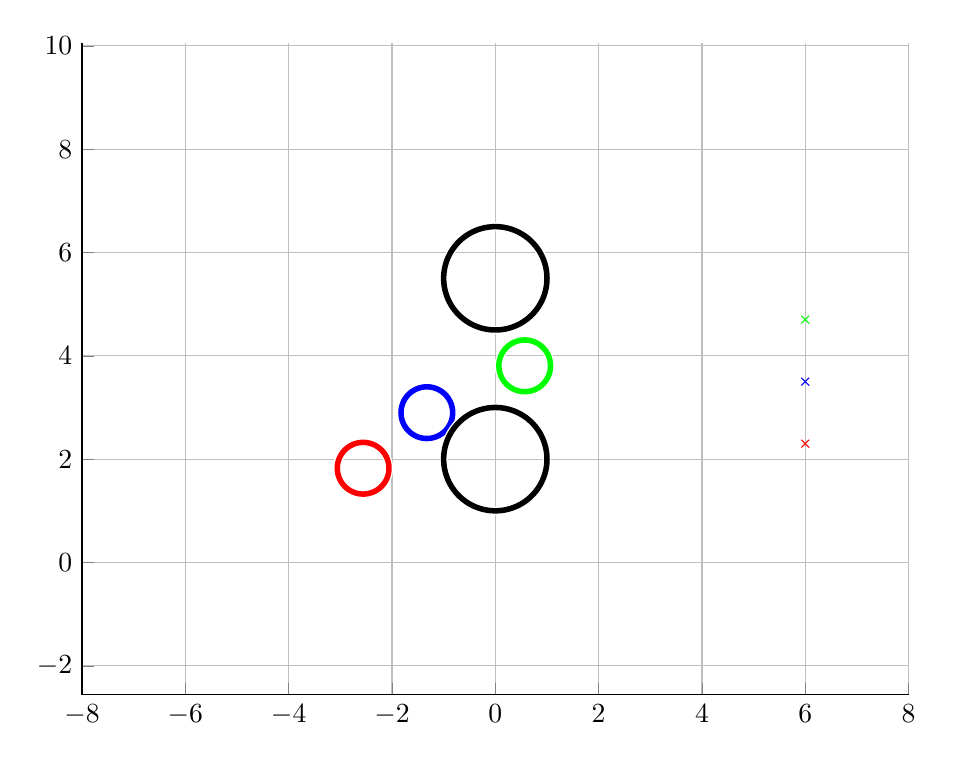
\begin{tikzpicture}

\begin{axis}[%
width=4.133in,
height=3.26in,
at={(0.693in,0.44in)},
scale only axis,
unbounded coords=jump,
xmin=-8,
xmax=8,
xmajorgrids,
ymin=-2.55967741935484,
ymax=10.0596774193548,
ymajorgrids,
axis background/.style={fill=white},
axis x line*=bottom,
axis y line*=left
]
\addplot [color=blue,only marks,mark=x,mark options={solid},forget plot]
  table[row sep=crcr]{%
6	3.5\\
};
\addplot [color=red,only marks,mark=x,mark options={solid},forget plot]
  table[row sep=crcr]{%
6	2.3\\
};
\addplot [color=green,only marks,mark=x,mark options={solid},forget plot]
  table[row sep=crcr]{%
6	4.7\\
};
\addplot [color=white,solid,line width=3.0pt,forget plot]
  table[row sep=crcr]{%
-0.825636227494789	2.89958553420376\\
-0.825940813985242	2.91703528255501\\
-0.826854202364877	2.93446377107582\\
-0.828375279810653	2.95184976583759\\
-0.830502193124004	2.96917208468379\\
-0.833232350988685	2.98640962303723\\
-0.836562427127887	3.00354137961264\\
-0.840488364356791	3.02054648200359\\
-0.84500537952563	3.03740421211226\\
-0.850107969347213	3.05409403139123\\
-0.855789917101835	3.07059560586659\\
-0.862044300211396	3.08688883091172\\
-0.868863498673489	3.10295385574166\\
-0.876239204345206	3.1187711075983\\
-0.884162431065326	3.13432131559671\\
-0.89262352560257	3.14958553420376\\
-0.901612179416577	3.16454516632036\\
-0.911117441217269	3.17918198593913\\
-0.921127730307316	3.19347816035\\
-0.931630850691428	3.20741627186659\\
-0.942614005935301	3.22097933904703\\
-0.954063814756092	3.23415083738319\\
-0.965966327325464	3.24691471943326\\
-0.978307042265291	3.25925543437309\\
-0.99107092431536	3.27115794694246\\
-1.00424242265152	3.28260775576325\\
-1.01780548983196	3.29359091100712\\
-1.03174360134855	3.30409403139123\\
-1.04603977575942	3.31410432048128\\
-1.06067659537819	3.32360958228197\\
-1.07563622749479	3.33259823609598\\
-1.09090044610184	3.34105933063322\\
-1.10645065410025	3.34898255735334\\
-1.12226790595689	3.35635826302506\\
-1.13833293078683	3.36317746148715\\
-1.15462615583196	3.36943184459671\\
-1.17112773030732	3.37511379235134\\
-1.18781754958629	3.38021638217292\\
-1.20467527969496	3.38473339734176\\
-1.22168038208591	3.38865933457066\\
-1.23881213866132	3.39198941070986\\
-1.25604967701476	3.39471956857455\\
-1.27337199586096	3.3968464818879\\
-1.29075799062273	3.39836755933367\\
-1.30818647914354	3.39928094771331\\
-1.32563622749479	3.39958553420376\\
-1.34308597584604	3.39928094771331\\
-1.36051446436685	3.39836755933367\\
-1.37790045912862	3.3968464818879\\
-1.39522277797482	3.39471956857455\\
-1.41246031632825	3.39198941070986\\
-1.42959207290367	3.38865933457066\\
-1.44659717529462	3.38473339734176\\
-1.46345490540329	3.38021638217292\\
-1.48014472468226	3.37511379235134\\
-1.49664629915762	3.36943184459671\\
-1.51293952420275	3.36317746148715\\
-1.52900454903269	3.35635826302506\\
-1.54482180088933	3.34898255735334\\
-1.56037200888773	3.34105933063322\\
-1.57563622749479	3.33259823609598\\
-1.59059585961139	3.32360958228197\\
-1.60523267923016	3.31410432048128\\
-1.61952885364103	3.30409403139123\\
-1.63346696515762	3.29359091100712\\
-1.64703003233806	3.28260775576325\\
-1.66020153067422	3.27115794694246\\
-1.67296541272429	3.25925543437309\\
-1.68530612766412	3.24691471943326\\
-1.69720864023349	3.23415083738319\\
-1.70865844905428	3.22097933904703\\
-1.71964160429815	3.20741627186659\\
-1.73014472468226	3.19347816035\\
-1.74015501377231	3.17918198593913\\
-1.749660275573	3.16454516632036\\
-1.75864892938701	3.14958553420376\\
-1.76711002392425	3.13432131559671\\
-1.77503325064437	3.1187711075983\\
-1.78240895631609	3.10295385574166\\
-1.78922815477818	3.08688883091172\\
-1.79548253788774	3.0705956058666\\
-1.80116448564237	3.05409403139123\\
-1.80626707546395	3.03740421211226\\
-1.81078409063279	3.02054648200359\\
-1.81471002786169	3.00354137961264\\
-1.81804010400089	2.98640962303723\\
-1.82077026186557	2.96917208468379\\
-1.82289717517893	2.95184976583759\\
-1.8244182526247	2.93446377107582\\
-1.82533164100434	2.91703528255501\\
-1.82563622749479	2.89958553420376\\
-1.82533164100434	2.88213578585251\\
-1.8244182526247	2.8647072973317\\
-1.82289717517893	2.84732130256993\\
-1.82077026186557	2.82999898372373\\
-1.81804010400089	2.8127614453703\\
-1.81471002786169	2.79562968879488\\
-1.81078409063279	2.77862458640393\\
-1.80626707546395	2.76176685629526\\
-1.80116448564237	2.74507703701629\\
-1.79548253788774	2.72857546254093\\
-1.78922815477818	2.7122822374958\\
-1.78240895631609	2.69621721266586\\
-1.77503325064437	2.68039996080922\\
-1.76711002392425	2.66484975281081\\
-1.75864892938701	2.64958553420376\\
-1.749660275573	2.63462590208716\\
-1.74015501377231	2.61998908246839\\
-1.73014472468226	2.60569290805752\\
-1.71964160429815	2.59175479654093\\
-1.70865844905428	2.57819172936049\\
-1.69720864023349	2.56502023102433\\
-1.68530612766412	2.55225634897426\\
-1.67296541272429	2.53991563403443\\
-1.66020153067422	2.52801312146506\\
-1.64703003233806	2.51656331264427\\
-1.63346696515762	2.5055801574004\\
-1.61952885364103	2.49507703701629\\
-1.60523267923016	2.48506674792624\\
-1.59059585961139	2.47556148612555\\
-1.57563622749479	2.46657283231154\\
-1.56037200888773	2.4581117377743\\
-1.54482180088933	2.45018851105418\\
-1.52900454903269	2.44281280538246\\
-1.51293952420275	2.43599360692037\\
-1.49664629915762	2.42973922381081\\
-1.48014472468226	2.42405727605618\\
-1.46345490540329	2.4189546862346\\
-1.44659717529462	2.41443767106576\\
-1.42959207290367	2.41051173383686\\
-1.41246031632825	2.40718165769766\\
-1.39522277797482	2.40445149983298\\
-1.37790045912862	2.40232458651962\\
-1.36051446436685	2.40080350907385\\
-1.34308597584604	2.39989012069421\\
-1.32563622749479	2.39958553420376\\
-1.30818647914354	2.39989012069421\\
-1.29075799062273	2.40080350907385\\
-1.27337199586096	2.40232458651962\\
-1.25604967701476	2.40445149983298\\
-1.23881213866132	2.40718165769766\\
-1.22168038208591	2.41051173383686\\
-1.20467527969496	2.41443767106576\\
-1.18781754958629	2.4189546862346\\
-1.17112773030732	2.42405727605618\\
-1.15462615583196	2.42973922381081\\
-1.13833293078683	2.43599360692037\\
-1.12226790595689	2.44281280538246\\
-1.10645065410025	2.45018851105418\\
-1.09090044610184	2.4581117377743\\
-1.07563622749479	2.46657283231154\\
-1.06067659537819	2.47556148612555\\
-1.04603977575942	2.48506674792624\\
-1.03174360134855	2.49507703701629\\
-1.01780548983196	2.5055801574004\\
-1.00424242265152	2.51656331264427\\
-0.991070924315361	2.52801312146506\\
-0.978307042265291	2.53991563403443\\
-0.965966327325464	2.55225634897426\\
-0.954063814756092	2.56502023102433\\
-0.942614005935301	2.57819172936049\\
-0.931630850691429	2.59175479654093\\
-0.921127730307316	2.60569290805752\\
-0.911117441217269	2.61998908246839\\
-0.901612179416577	2.63462590208716\\
-0.89262352560257	2.64958553420376\\
-0.884162431065326	2.66484975281081\\
-0.876239204345206	2.68039996080922\\
-0.868863498673489	2.69621721266586\\
-0.862044300211396	2.7122822374958\\
-0.855789917101835	2.72857546254093\\
-0.850107969347213	2.74507703701629\\
-0.84500537952563	2.76176685629526\\
-0.840488364356791	2.77862458640393\\
-0.836562427127887	2.79562968879488\\
-0.833232350988686	2.81276144537029\\
-0.830502193124004	2.82999898372373\\
-0.828375279810653	2.84732130256993\\
-0.826854202364877	2.8647072973317\\
-0.825940813985242	2.88213578585251\\
-0.825636227494789	2.89958553420376\\
nan	nan\\
};
\addplot [color=blue,solid,line width=2.0pt,forget plot]
  table[row sep=crcr]{%
-0.825636227494789	2.89958553420376\\
-0.825940813985242	2.91703528255501\\
-0.826854202364877	2.93446377107582\\
-0.828375279810653	2.95184976583759\\
-0.830502193124004	2.96917208468379\\
-0.833232350988685	2.98640962303723\\
-0.836562427127887	3.00354137961264\\
-0.840488364356791	3.02054648200359\\
-0.84500537952563	3.03740421211226\\
-0.850107969347213	3.05409403139123\\
-0.855789917101835	3.07059560586659\\
-0.862044300211396	3.08688883091172\\
-0.868863498673489	3.10295385574166\\
-0.876239204345206	3.1187711075983\\
-0.884162431065326	3.13432131559671\\
-0.89262352560257	3.14958553420376\\
-0.901612179416577	3.16454516632036\\
-0.911117441217269	3.17918198593913\\
-0.921127730307316	3.19347816035\\
-0.931630850691428	3.20741627186659\\
-0.942614005935301	3.22097933904703\\
-0.954063814756092	3.23415083738319\\
-0.965966327325464	3.24691471943326\\
-0.978307042265291	3.25925543437309\\
-0.99107092431536	3.27115794694246\\
-1.00424242265152	3.28260775576325\\
-1.01780548983196	3.29359091100712\\
-1.03174360134855	3.30409403139123\\
-1.04603977575942	3.31410432048128\\
-1.06067659537819	3.32360958228197\\
-1.07563622749479	3.33259823609598\\
-1.09090044610184	3.34105933063322\\
-1.10645065410025	3.34898255735334\\
-1.12226790595689	3.35635826302506\\
-1.13833293078683	3.36317746148715\\
-1.15462615583196	3.36943184459671\\
-1.17112773030732	3.37511379235134\\
-1.18781754958629	3.38021638217292\\
-1.20467527969496	3.38473339734176\\
-1.22168038208591	3.38865933457066\\
-1.23881213866132	3.39198941070986\\
-1.25604967701476	3.39471956857455\\
-1.27337199586096	3.3968464818879\\
-1.29075799062273	3.39836755933367\\
-1.30818647914354	3.39928094771331\\
-1.32563622749479	3.39958553420376\\
-1.34308597584604	3.39928094771331\\
-1.36051446436685	3.39836755933367\\
-1.37790045912862	3.3968464818879\\
-1.39522277797482	3.39471956857455\\
-1.41246031632825	3.39198941070986\\
-1.42959207290367	3.38865933457066\\
-1.44659717529462	3.38473339734176\\
-1.46345490540329	3.38021638217292\\
-1.48014472468226	3.37511379235134\\
-1.49664629915762	3.36943184459671\\
-1.51293952420275	3.36317746148715\\
-1.52900454903269	3.35635826302506\\
-1.54482180088933	3.34898255735334\\
-1.56037200888773	3.34105933063322\\
-1.57563622749479	3.33259823609598\\
-1.59059585961139	3.32360958228197\\
-1.60523267923016	3.31410432048128\\
-1.61952885364103	3.30409403139123\\
-1.63346696515762	3.29359091100712\\
-1.64703003233806	3.28260775576325\\
-1.66020153067422	3.27115794694246\\
-1.67296541272429	3.25925543437309\\
-1.68530612766412	3.24691471943326\\
-1.69720864023349	3.23415083738319\\
-1.70865844905428	3.22097933904703\\
-1.71964160429815	3.20741627186659\\
-1.73014472468226	3.19347816035\\
-1.74015501377231	3.17918198593913\\
-1.749660275573	3.16454516632036\\
-1.75864892938701	3.14958553420376\\
-1.76711002392425	3.13432131559671\\
-1.77503325064437	3.1187711075983\\
-1.78240895631609	3.10295385574166\\
-1.78922815477818	3.08688883091172\\
-1.79548253788774	3.0705956058666\\
-1.80116448564237	3.05409403139123\\
-1.80626707546395	3.03740421211226\\
-1.81078409063279	3.02054648200359\\
-1.81471002786169	3.00354137961264\\
-1.81804010400089	2.98640962303723\\
-1.82077026186557	2.96917208468379\\
-1.82289717517893	2.95184976583759\\
-1.8244182526247	2.93446377107582\\
-1.82533164100434	2.91703528255501\\
-1.82563622749479	2.89958553420376\\
-1.82533164100434	2.88213578585251\\
-1.8244182526247	2.8647072973317\\
-1.82289717517893	2.84732130256993\\
-1.82077026186557	2.82999898372373\\
-1.81804010400089	2.8127614453703\\
-1.81471002786169	2.79562968879488\\
-1.81078409063279	2.77862458640393\\
-1.80626707546395	2.76176685629526\\
-1.80116448564237	2.74507703701629\\
-1.79548253788774	2.72857546254093\\
-1.78922815477818	2.7122822374958\\
-1.78240895631609	2.69621721266586\\
-1.77503325064437	2.68039996080922\\
-1.76711002392425	2.66484975281081\\
-1.75864892938701	2.64958553420376\\
-1.749660275573	2.63462590208716\\
-1.74015501377231	2.61998908246839\\
-1.73014472468226	2.60569290805752\\
-1.71964160429815	2.59175479654093\\
-1.70865844905428	2.57819172936049\\
-1.69720864023349	2.56502023102433\\
-1.68530612766412	2.55225634897426\\
-1.67296541272429	2.53991563403443\\
-1.66020153067422	2.52801312146506\\
-1.64703003233806	2.51656331264427\\
-1.63346696515762	2.5055801574004\\
-1.61952885364103	2.49507703701629\\
-1.60523267923016	2.48506674792624\\
-1.59059585961139	2.47556148612555\\
-1.57563622749479	2.46657283231154\\
-1.56037200888773	2.4581117377743\\
-1.54482180088933	2.45018851105418\\
-1.52900454903269	2.44281280538246\\
-1.51293952420275	2.43599360692037\\
-1.49664629915762	2.42973922381081\\
-1.48014472468226	2.42405727605618\\
-1.46345490540329	2.4189546862346\\
-1.44659717529462	2.41443767106576\\
-1.42959207290367	2.41051173383686\\
-1.41246031632825	2.40718165769766\\
-1.39522277797482	2.40445149983298\\
-1.37790045912862	2.40232458651962\\
-1.36051446436685	2.40080350907385\\
-1.34308597584604	2.39989012069421\\
-1.32563622749479	2.39958553420376\\
-1.30818647914354	2.39989012069421\\
-1.29075799062273	2.40080350907385\\
-1.27337199586096	2.40232458651962\\
-1.25604967701476	2.40445149983298\\
-1.23881213866132	2.40718165769766\\
-1.22168038208591	2.41051173383686\\
-1.20467527969496	2.41443767106576\\
-1.18781754958629	2.4189546862346\\
-1.17112773030732	2.42405727605618\\
-1.15462615583196	2.42973922381081\\
-1.13833293078683	2.43599360692037\\
-1.12226790595689	2.44281280538246\\
-1.10645065410025	2.45018851105418\\
-1.09090044610184	2.4581117377743\\
-1.07563622749479	2.46657283231154\\
-1.06067659537819	2.47556148612555\\
-1.04603977575942	2.48506674792624\\
-1.03174360134855	2.49507703701629\\
-1.01780548983196	2.5055801574004\\
-1.00424242265152	2.51656331264427\\
-0.991070924315361	2.52801312146506\\
-0.978307042265291	2.53991563403443\\
-0.965966327325464	2.55225634897426\\
-0.954063814756092	2.56502023102433\\
-0.942614005935301	2.57819172936049\\
-0.931630850691429	2.59175479654093\\
-0.921127730307316	2.60569290805752\\
-0.911117441217269	2.61998908246839\\
-0.901612179416577	2.63462590208716\\
-0.89262352560257	2.64958553420376\\
-0.884162431065326	2.66484975281081\\
-0.876239204345206	2.68039996080922\\
-0.868863498673489	2.69621721266586\\
-0.862044300211396	2.7122822374958\\
-0.855789917101835	2.72857546254093\\
-0.850107969347213	2.74507703701629\\
-0.84500537952563	2.76176685629526\\
-0.840488364356791	2.77862458640393\\
-0.836562427127887	2.79562968879488\\
-0.833232350988686	2.81276144537029\\
-0.830502193124004	2.82999898372373\\
-0.828375279810653	2.84732130256993\\
-0.826854202364877	2.8647072973317\\
-0.825940813985242	2.88213578585251\\
-0.825636227494789	2.89958553420376\\
nan	nan\\
};
\addplot [color=white,solid,line width=3.0pt,forget plot]
  table[row sep=crcr]{%
-2.05864166187496	1.82449303348009\\
-2.05894624836541	1.84194278183134\\
-2.05985963674504	1.85937127035215\\
-2.06138071419082	1.87675726511392\\
-2.06350762750417	1.89407958396012\\
-2.06623778536885	1.91131712231355\\
-2.06956786150805	1.92844887888897\\
-2.07349379873696	1.94545398127992\\
-2.0780108139058	1.96231171138859\\
-2.08311340372738	1.97900153066756\\
-2.088795351482	1.99550310514292\\
-2.09504973459156	2.01179633018805\\
-2.10186893305366	2.02786135501799\\
-2.10924463872537	2.04367860687463\\
-2.11716786544549	2.05922881487303\\
-2.12562895998274	2.07449303348009\\
-2.13461761379674	2.08945266559669\\
-2.14412287559744	2.10408948521546\\
-2.15413316468748	2.11838565962633\\
-2.1646362850716	2.13232377114292\\
-2.17561944031547	2.14588683832336\\
-2.18706924913626	2.15905833665952\\
-2.19897176170563	2.17182221870959\\
-2.21131247664546	2.18416293364942\\
-2.22407635869553	2.19606544621879\\
-2.23724785703169	2.20751525503958\\
-2.25081092421213	2.21849841028345\\
-2.26474903572872	2.22900153066756\\
-2.27904521013958	2.23901181975761\\
-2.29368202975835	2.2485170815583\\
-2.30864166187496	2.25750573537231\\
-2.32390588048201	2.26596682990955\\
-2.33945608848042	2.27389005662967\\
-2.35527334033706	2.28126576230139\\
-2.371338365167	2.28808496076348\\
-2.38763159021212	2.29433934387304\\
-2.40413316468748	2.30002129162767\\
-2.42082298396646	2.30512388144925\\
-2.43768071407512	2.30964089661809\\
-2.45468581646608	2.31356683384699\\
-2.47181757304149	2.31689690998619\\
-2.48905511139492	2.31962706785087\\
-2.50637743024113	2.32175398116423\\
-2.52376342500289	2.32327505861\\
-2.54119191352371	2.32418844698964\\
-2.55864166187496	2.32449303348009\\
-2.57609141022621	2.32418844698964\\
-2.59351989874702	2.32327505861\\
-2.61090589350878	2.32175398116423\\
-2.62822821235499	2.31962706785087\\
-2.64546575070842	2.31689690998619\\
-2.66259750728384	2.31356683384699\\
-2.67960260967479	2.30964089661809\\
-2.69646033978346	2.30512388144925\\
-2.71315015906243	2.30002129162767\\
-2.72965173353779	2.29433934387304\\
-2.74594495858291	2.28808496076348\\
-2.76200998341286	2.28126576230139\\
-2.7778272352695	2.27389005662967\\
-2.7933774432679	2.26596682990955\\
-2.80864166187496	2.25750573537231\\
-2.82360129399156	2.2485170815583\\
-2.83823811361033	2.23901181975761\\
-2.85253428802119	2.22900153066756\\
-2.86647239953779	2.21849841028345\\
-2.88003546671823	2.20751525503958\\
-2.89320696505439	2.19606544621879\\
-2.90597084710445	2.18416293364942\\
-2.91831156204428	2.17182221870959\\
-2.93021407461365	2.15905833665952\\
-2.94166388343445	2.14588683832336\\
-2.95264703867832	2.13232377114292\\
-2.96315015906243	2.11838565962633\\
-2.97316044815248	2.10408948521546\\
-2.98266570995317	2.08945266559669\\
-2.99165436376718	2.07449303348009\\
-3.00011545830442	2.05922881487303\\
-3.00803868502454	2.04367860687463\\
-3.01541439069626	2.02786135501799\\
-3.02223358915835	2.01179633018805\\
-3.02848797226791	1.99550310514292\\
-3.03416992002253	1.97900153066756\\
-3.03927250984412	1.96231171138859\\
-3.04378952501295	1.94545398127992\\
-3.04771546224186	1.92844887888897\\
-3.05104553838106	1.91131712231355\\
-3.05377569624574	1.89407958396012\\
-3.05590260955909	1.87675726511392\\
-3.05742368700487	1.85937127035215\\
-3.0583370753845	1.84194278183134\\
-3.05864166187496	1.82449303348009\\
-3.0583370753845	1.80704328512884\\
-3.05742368700487	1.78961479660803\\
-3.05590260955909	1.77222880184626\\
-3.05377569624574	1.75490648300006\\
-3.05104553838106	1.73766894464662\\
-3.04771546224186	1.72053718807121\\
-3.04378952501295	1.70353208568026\\
-3.03927250984412	1.68667435557159\\
-3.03416992002253	1.66998453629262\\
-3.02848797226791	1.65348296181726\\
-3.02223358915835	1.63718973677213\\
-3.01541439069626	1.62112471194219\\
-3.00803868502454	1.60530746008555\\
-3.00011545830442	1.58975725208714\\
-2.99165436376718	1.57449303348009\\
-2.98266570995317	1.55953340136349\\
-2.97316044815248	1.54489658174472\\
-2.96315015906243	1.53060040733385\\
-2.95264703867832	1.51666229581726\\
-2.94166388343445	1.50309922863682\\
-2.93021407461365	1.48992773030066\\
-2.91831156204428	1.47716384825059\\
-2.90597084710445	1.46482313331076\\
-2.89320696505439	1.45292062074139\\
-2.88003546671823	1.4414708119206\\
-2.86647239953779	1.43048765667673\\
-2.85253428802119	1.41998453629262\\
-2.83823811361033	1.40997424720257\\
-2.82360129399156	1.40046898540188\\
-2.80864166187496	1.39148033158787\\
-2.7933774432679	1.38301923705063\\
-2.7778272352695	1.37509601033051\\
-2.76200998341286	1.36772030465879\\
-2.74594495858291	1.3609011061967\\
-2.72965173353779	1.35464672308714\\
-2.71315015906243	1.34896477533251\\
-2.69646033978346	1.34386218551093\\
-2.67960260967479	1.33934517034209\\
-2.66259750728384	1.33541923311319\\
-2.64546575070842	1.33208915697399\\
-2.62822821235499	1.3293589991093\\
-2.61090589350878	1.32723208579595\\
-2.59351989874702	1.32571100835018\\
-2.57609141022621	1.32479761997054\\
-2.55864166187496	1.32449303348009\\
-2.54119191352371	1.32479761997054\\
-2.52376342500289	1.32571100835018\\
-2.50637743024113	1.32723208579595\\
-2.48905511139492	1.3293589991093\\
-2.47181757304149	1.33208915697399\\
-2.45468581646608	1.33541923311319\\
-2.43768071407512	1.33934517034209\\
-2.42082298396646	1.34386218551093\\
-2.40413316468748	1.34896477533251\\
-2.38763159021212	1.35464672308714\\
-2.371338365167	1.3609011061967\\
-2.35527334033706	1.36772030465879\\
-2.33945608848042	1.37509601033051\\
-2.32390588048201	1.38301923705063\\
-2.30864166187496	1.39148033158787\\
-2.29368202975835	1.40046898540188\\
-2.27904521013958	1.40997424720257\\
-2.26474903572872	1.41998453629262\\
-2.25081092421213	1.43048765667673\\
-2.23724785703169	1.4414708119206\\
-2.22407635869553	1.45292062074139\\
-2.21131247664546	1.46482313331076\\
-2.19897176170563	1.47716384825059\\
-2.18706924913626	1.48992773030066\\
-2.17561944031547	1.50309922863682\\
-2.1646362850716	1.51666229581726\\
-2.15413316468748	1.53060040733385\\
-2.14412287559744	1.54489658174472\\
-2.13461761379674	1.55953340136349\\
-2.12562895998274	1.57449303348009\\
-2.11716786544549	1.58975725208714\\
-2.10924463872537	1.60530746008555\\
-2.10186893305366	1.62112471194219\\
-2.09504973459156	1.63718973677213\\
-2.088795351482	1.65348296181726\\
-2.08311340372738	1.66998453629262\\
-2.0780108139058	1.68667435557159\\
-2.07349379873696	1.70353208568026\\
-2.06956786150805	1.72053718807121\\
-2.06623778536885	1.73766894464662\\
-2.06350762750417	1.75490648300006\\
-2.06138071419082	1.77222880184626\\
-2.05985963674504	1.78961479660803\\
-2.05894624836541	1.80704328512884\\
-2.05864166187496	1.82449303348009\\
nan	nan\\
};
\addplot [color=red,solid,line width=2.0pt,forget plot]
  table[row sep=crcr]{%
-2.05864166187496	1.82449303348009\\
-2.05894624836541	1.84194278183134\\
-2.05985963674504	1.85937127035215\\
-2.06138071419082	1.87675726511392\\
-2.06350762750417	1.89407958396012\\
-2.06623778536885	1.91131712231355\\
-2.06956786150805	1.92844887888897\\
-2.07349379873696	1.94545398127992\\
-2.0780108139058	1.96231171138859\\
-2.08311340372738	1.97900153066756\\
-2.088795351482	1.99550310514292\\
-2.09504973459156	2.01179633018805\\
-2.10186893305366	2.02786135501799\\
-2.10924463872537	2.04367860687463\\
-2.11716786544549	2.05922881487303\\
-2.12562895998274	2.07449303348009\\
-2.13461761379674	2.08945266559669\\
-2.14412287559744	2.10408948521546\\
-2.15413316468748	2.11838565962633\\
-2.1646362850716	2.13232377114292\\
-2.17561944031547	2.14588683832336\\
-2.18706924913626	2.15905833665952\\
-2.19897176170563	2.17182221870959\\
-2.21131247664546	2.18416293364942\\
-2.22407635869553	2.19606544621879\\
-2.23724785703169	2.20751525503958\\
-2.25081092421213	2.21849841028345\\
-2.26474903572872	2.22900153066756\\
-2.27904521013958	2.23901181975761\\
-2.29368202975835	2.2485170815583\\
-2.30864166187496	2.25750573537231\\
-2.32390588048201	2.26596682990955\\
-2.33945608848042	2.27389005662967\\
-2.35527334033706	2.28126576230139\\
-2.371338365167	2.28808496076348\\
-2.38763159021212	2.29433934387304\\
-2.40413316468748	2.30002129162767\\
-2.42082298396646	2.30512388144925\\
-2.43768071407512	2.30964089661809\\
-2.45468581646608	2.31356683384699\\
-2.47181757304149	2.31689690998619\\
-2.48905511139492	2.31962706785087\\
-2.50637743024113	2.32175398116423\\
-2.52376342500289	2.32327505861\\
-2.54119191352371	2.32418844698964\\
-2.55864166187496	2.32449303348009\\
-2.57609141022621	2.32418844698964\\
-2.59351989874702	2.32327505861\\
-2.61090589350878	2.32175398116423\\
-2.62822821235499	2.31962706785087\\
-2.64546575070842	2.31689690998619\\
-2.66259750728384	2.31356683384699\\
-2.67960260967479	2.30964089661809\\
-2.69646033978346	2.30512388144925\\
-2.71315015906243	2.30002129162767\\
-2.72965173353779	2.29433934387304\\
-2.74594495858291	2.28808496076348\\
-2.76200998341286	2.28126576230139\\
-2.7778272352695	2.27389005662967\\
-2.7933774432679	2.26596682990955\\
-2.80864166187496	2.25750573537231\\
-2.82360129399156	2.2485170815583\\
-2.83823811361033	2.23901181975761\\
-2.85253428802119	2.22900153066756\\
-2.86647239953779	2.21849841028345\\
-2.88003546671823	2.20751525503958\\
-2.89320696505439	2.19606544621879\\
-2.90597084710445	2.18416293364942\\
-2.91831156204428	2.17182221870959\\
-2.93021407461365	2.15905833665952\\
-2.94166388343445	2.14588683832336\\
-2.95264703867832	2.13232377114292\\
-2.96315015906243	2.11838565962633\\
-2.97316044815248	2.10408948521546\\
-2.98266570995317	2.08945266559669\\
-2.99165436376718	2.07449303348009\\
-3.00011545830442	2.05922881487303\\
-3.00803868502454	2.04367860687463\\
-3.01541439069626	2.02786135501799\\
-3.02223358915835	2.01179633018805\\
-3.02848797226791	1.99550310514292\\
-3.03416992002253	1.97900153066756\\
-3.03927250984412	1.96231171138859\\
-3.04378952501295	1.94545398127992\\
-3.04771546224186	1.92844887888897\\
-3.05104553838106	1.91131712231355\\
-3.05377569624574	1.89407958396012\\
-3.05590260955909	1.87675726511392\\
-3.05742368700487	1.85937127035215\\
-3.0583370753845	1.84194278183134\\
-3.05864166187496	1.82449303348009\\
-3.0583370753845	1.80704328512884\\
-3.05742368700487	1.78961479660803\\
-3.05590260955909	1.77222880184626\\
-3.05377569624574	1.75490648300006\\
-3.05104553838106	1.73766894464662\\
-3.04771546224186	1.72053718807121\\
-3.04378952501295	1.70353208568026\\
-3.03927250984412	1.68667435557159\\
-3.03416992002253	1.66998453629262\\
-3.02848797226791	1.65348296181726\\
-3.02223358915835	1.63718973677213\\
-3.01541439069626	1.62112471194219\\
-3.00803868502454	1.60530746008555\\
-3.00011545830442	1.58975725208714\\
-2.99165436376718	1.57449303348009\\
-2.98266570995317	1.55953340136349\\
-2.97316044815248	1.54489658174472\\
-2.96315015906243	1.53060040733385\\
-2.95264703867832	1.51666229581726\\
-2.94166388343445	1.50309922863682\\
-2.93021407461365	1.48992773030066\\
-2.91831156204428	1.47716384825059\\
-2.90597084710445	1.46482313331076\\
-2.89320696505439	1.45292062074139\\
-2.88003546671823	1.4414708119206\\
-2.86647239953779	1.43048765667673\\
-2.85253428802119	1.41998453629262\\
-2.83823811361033	1.40997424720257\\
-2.82360129399156	1.40046898540188\\
-2.80864166187496	1.39148033158787\\
-2.7933774432679	1.38301923705063\\
-2.7778272352695	1.37509601033051\\
-2.76200998341286	1.36772030465879\\
-2.74594495858291	1.3609011061967\\
-2.72965173353779	1.35464672308714\\
-2.71315015906243	1.34896477533251\\
-2.69646033978346	1.34386218551093\\
-2.67960260967479	1.33934517034209\\
-2.66259750728384	1.33541923311319\\
-2.64546575070842	1.33208915697399\\
-2.62822821235499	1.3293589991093\\
-2.61090589350878	1.32723208579595\\
-2.59351989874702	1.32571100835018\\
-2.57609141022621	1.32479761997054\\
-2.55864166187496	1.32449303348009\\
-2.54119191352371	1.32479761997054\\
-2.52376342500289	1.32571100835018\\
-2.50637743024113	1.32723208579595\\
-2.48905511139492	1.3293589991093\\
-2.47181757304149	1.33208915697399\\
-2.45468581646608	1.33541923311319\\
-2.43768071407512	1.33934517034209\\
-2.42082298396646	1.34386218551093\\
-2.40413316468748	1.34896477533251\\
-2.38763159021212	1.35464672308714\\
-2.371338365167	1.3609011061967\\
-2.35527334033706	1.36772030465879\\
-2.33945608848042	1.37509601033051\\
-2.32390588048201	1.38301923705063\\
-2.30864166187496	1.39148033158787\\
-2.29368202975835	1.40046898540188\\
-2.27904521013958	1.40997424720257\\
-2.26474903572872	1.41998453629262\\
-2.25081092421213	1.43048765667673\\
-2.23724785703169	1.4414708119206\\
-2.22407635869553	1.45292062074139\\
-2.21131247664546	1.46482313331076\\
-2.19897176170563	1.47716384825059\\
-2.18706924913626	1.48992773030066\\
-2.17561944031547	1.50309922863682\\
-2.1646362850716	1.51666229581726\\
-2.15413316468748	1.53060040733385\\
-2.14412287559744	1.54489658174472\\
-2.13461761379674	1.55953340136349\\
-2.12562895998274	1.57449303348009\\
-2.11716786544549	1.58975725208714\\
-2.10924463872537	1.60530746008555\\
-2.10186893305366	1.62112471194219\\
-2.09504973459156	1.63718973677213\\
-2.088795351482	1.65348296181726\\
-2.08311340372738	1.66998453629262\\
-2.0780108139058	1.68667435557159\\
-2.07349379873696	1.70353208568026\\
-2.06956786150805	1.72053718807121\\
-2.06623778536885	1.73766894464662\\
-2.06350762750417	1.75490648300006\\
-2.06138071419082	1.77222880184626\\
-2.05985963674504	1.78961479660803\\
-2.05894624836541	1.80704328512884\\
-2.05864166187496	1.82449303348009\\
nan	nan\\
};
\addplot [color=white,solid,line width=3.0pt,forget plot]
  table[row sep=crcr]{%
1.06860844448809	3.80613786146227\\
1.06830385799764	3.82358760981352\\
1.067390469618	3.84101609833433\\
1.06586939217223	3.85840209309609\\
1.06374247885887	3.8757244119423\\
1.06101232099419	3.89296195029573\\
1.05768224485499	3.91009370687115\\
1.05375630762609	3.9270988092621\\
1.04923929245725	3.94395653937077\\
1.04413670263567	3.96064635864974\\
1.03845475488104	3.9771479331251\\
1.03220037177148	3.99344115817022\\
1.02538117330939	4.00950618300017\\
1.01800546763767	4.0253234348568\\
1.01008224091755	4.04087364285521\\
1.00162114638031	4.05613786146227\\
0.992632492566302	4.07109749357887\\
0.98312723076561	4.08573431319764\\
0.973116941675563	4.1000304876085\\
0.96261382129145	4.11396859912509\\
0.951630666047578	4.12753166630554\\
0.940180857226786	4.14070316464169\\
0.928278344657415	4.15346704669176\\
0.915937629717588	4.16580776163159\\
0.903173747667518	4.17771027420096\\
0.890002249331359	4.18916008302176\\
0.876439182150918	4.20014323826563\\
0.862501070634326	4.21064635864974\\
0.848204896223463	4.22065664773979\\
0.833568076604692	4.23016190954048\\
0.818608444488089	4.23915056335449\\
0.803344225881035	4.24761165789173\\
0.787794017882628	4.25553488461185\\
0.771976766025989	4.26291059028357\\
0.755911741196045	4.26972978874566\\
0.739618516150924	4.27598417185522\\
0.723116941675563	4.28166611960984\\
0.706427122396589	4.28676870943143\\
0.689569392287923	4.29128572460026\\
0.672564289896969	4.29521166182917\\
0.655432533321554	4.29854173796837\\
0.638194994968122	4.30127189583305\\
0.620872676121916	4.3033988091464\\
0.603486681360152	4.30491988659218\\
0.58605819283934	4.30583327497181\\
0.568608444488089	4.30613786146227\\
0.551158696136839	4.30583327497181\\
0.533730207616027	4.30491988659218\\
0.516344212854263	4.3033988091464\\
0.499021894008057	4.30127189583305\\
0.481784355654624	4.29854173796837\\
0.46465259907921	4.29521166182917\\
0.447647496688255	4.29128572460026\\
0.43078976657959	4.28676870943143\\
0.414099947300616	4.28166611960984\\
0.397598372825255	4.27598417185522\\
0.381305147780133	4.26972978874566\\
0.365240122950189	4.26291059028357\\
0.34942287109355	4.25553488461185\\
0.333872663095144	4.24761165789173\\
0.318608444488089	4.23915056335449\\
0.303648812371487	4.23016190954048\\
0.289011992752716	4.22065664773979\\
0.274715818341853	4.21064635864974\\
0.26077770682526	4.20014323826563\\
0.24721463964482	4.18916008302176\\
0.23404314130866	4.17771027420096\\
0.221279259258591	4.16580776163159\\
0.208938544318764	4.15346704669176\\
0.197036031749392	4.1407031646417\\
0.1855862229286	4.12753166630554\\
0.174603067684728	4.1139685991251\\
0.164099947300616	4.1000304876085\\
0.154089658210568	4.08573431319764\\
0.144584396409876	4.07109749357887\\
0.13559574259587	4.05613786146227\\
0.127134648058626	4.04087364285521\\
0.119211421338506	4.0253234348568\\
0.111835715666789	4.00950618300017\\
0.105016517204696	3.99344115817022\\
0.0987621340951351	3.9771479331251\\
0.0930801863405125	3.96064635864974\\
0.0879775965189299	3.94395653937077\\
0.083460581350091	3.9270988092621\\
0.0795346441211864	3.91009370687115\\
0.0762045679819852	3.89296195029573\\
0.0734744101173041	3.8757244119423\\
0.0713474968039526	3.85840209309609\\
0.0698264193581771	3.84101609833433\\
0.0689130309785413	3.82358760981352\\
0.0686084444880892	3.80613786146227\\
0.0689130309785413	3.78868811311102\\
0.0698264193581771	3.7712596245902\\
0.0713474968039525	3.75387362982844\\
0.0734744101173041	3.73655131098223\\
0.0762045679819852	3.7193137726288\\
0.0795346441211864	3.70218201605339\\
0.0834605813500909	3.68517691366243\\
0.0879775965189298	3.66831918355377\\
0.0930801863405125	3.65162936427479\\
0.098762134095135	3.63512778979943\\
0.105016517204696	3.61883456475431\\
0.111835715666789	3.60276953992437\\
0.119211421338506	3.58695228806773\\
0.127134648058626	3.57140208006932\\
0.13559574259587	3.55613786146227\\
0.144584396409876	3.54117822934566\\
0.154089658210568	3.52654140972689\\
0.164099947300616	3.51224523531603\\
0.174603067684728	3.49830712379944\\
0.1855862229286	3.484744056619\\
0.197036031749392	3.47157255828284\\
0.208938544318764	3.45880867623277\\
0.22127925925859	3.44646796129294\\
0.23404314130866	3.43456544872357\\
0.247214639644819	3.42311563990278\\
0.26077770682526	3.4121324846589\\
0.274715818341853	3.40162936427479\\
0.289011992752716	3.39161907518475\\
0.303648812371487	3.38211381338405\\
0.318608444488089	3.37312515957005\\
0.333872663095144	3.3646640650328\\
0.34942287109355	3.35674083831268\\
0.365240122950189	3.34936513264097\\
0.381305147780133	3.34254593417887\\
0.397598372825255	3.33629155106931\\
0.414099947300615	3.33060960331469\\
0.43078976657959	3.32550701349311\\
0.447647496688255	3.32098999832427\\
0.464652599079209	3.31706406109536\\
0.481784355654624	3.31373398495616\\
0.499021894008057	3.31100382709148\\
0.516344212854263	3.30887691377813\\
0.533730207616026	3.30735583633235\\
0.551158696136838	3.30644244795272\\
0.568608444488089	3.30613786146227\\
0.58605819283934	3.30644244795272\\
0.603486681360152	3.30735583633235\\
0.620872676121916	3.30887691377813\\
0.638194994968122	3.31100382709148\\
0.655432533321554	3.31373398495616\\
0.672564289896968	3.31706406109536\\
0.689569392287923	3.32098999832427\\
0.706427122396589	3.32550701349311\\
0.723116941675563	3.33060960331469\\
0.739618516150923	3.33629155106931\\
0.755911741196045	3.34254593417887\\
0.77197676602599	3.34936513264097\\
0.787794017882628	3.35674083831268\\
0.803344225881034	3.3646640650328\\
0.818608444488089	3.37312515957005\\
0.833568076604692	3.38211381338405\\
0.848204896223462	3.39161907518474\\
0.862501070634326	3.40162936427479\\
0.876439182150919	3.4121324846589\\
0.890002249331359	3.42311563990278\\
0.903173747667518	3.43456544872357\\
0.915937629717588	3.44646796129294\\
0.928278344657415	3.45880867623277\\
0.940180857226786	3.47157255828284\\
0.951630666047578	3.484744056619\\
0.96261382129145	3.49830712379944\\
0.973116941675563	3.51224523531603\\
0.98312723076561	3.52654140972689\\
0.992632492566302	3.54117822934566\\
1.00162114638031	3.55613786146227\\
1.01008224091755	3.57140208006932\\
1.01800546763767	3.58695228806773\\
1.02538117330939	3.60276953992437\\
1.03220037177148	3.61883456475431\\
1.03845475488104	3.63512778979943\\
1.04413670263567	3.65162936427479\\
1.04923929245725	3.66831918355377\\
1.05375630762609	3.68517691366243\\
1.05768224485499	3.70218201605339\\
1.06101232099419	3.7193137726288\\
1.06374247885887	3.73655131098223\\
1.06586939217223	3.75387362982844\\
1.067390469618	3.7712596245902\\
1.06830385799764	3.78868811311102\\
1.06860844448809	3.80613786146227\\
nan	nan\\
};
\addplot [color=green,solid,line width=2.0pt,forget plot]
  table[row sep=crcr]{%
1.06860844448809	3.80613786146227\\
1.06830385799764	3.82358760981352\\
1.067390469618	3.84101609833433\\
1.06586939217223	3.85840209309609\\
1.06374247885887	3.8757244119423\\
1.06101232099419	3.89296195029573\\
1.05768224485499	3.91009370687115\\
1.05375630762609	3.9270988092621\\
1.04923929245725	3.94395653937077\\
1.04413670263567	3.96064635864974\\
1.03845475488104	3.9771479331251\\
1.03220037177148	3.99344115817022\\
1.02538117330939	4.00950618300017\\
1.01800546763767	4.0253234348568\\
1.01008224091755	4.04087364285521\\
1.00162114638031	4.05613786146227\\
0.992632492566302	4.07109749357887\\
0.98312723076561	4.08573431319764\\
0.973116941675563	4.1000304876085\\
0.96261382129145	4.11396859912509\\
0.951630666047578	4.12753166630554\\
0.940180857226786	4.14070316464169\\
0.928278344657415	4.15346704669176\\
0.915937629717588	4.16580776163159\\
0.903173747667518	4.17771027420096\\
0.890002249331359	4.18916008302176\\
0.876439182150918	4.20014323826563\\
0.862501070634326	4.21064635864974\\
0.848204896223463	4.22065664773979\\
0.833568076604692	4.23016190954048\\
0.818608444488089	4.23915056335449\\
0.803344225881035	4.24761165789173\\
0.787794017882628	4.25553488461185\\
0.771976766025989	4.26291059028357\\
0.755911741196045	4.26972978874566\\
0.739618516150924	4.27598417185522\\
0.723116941675563	4.28166611960984\\
0.706427122396589	4.28676870943143\\
0.689569392287923	4.29128572460026\\
0.672564289896969	4.29521166182917\\
0.655432533321554	4.29854173796837\\
0.638194994968122	4.30127189583305\\
0.620872676121916	4.3033988091464\\
0.603486681360152	4.30491988659218\\
0.58605819283934	4.30583327497181\\
0.568608444488089	4.30613786146227\\
0.551158696136839	4.30583327497181\\
0.533730207616027	4.30491988659218\\
0.516344212854263	4.3033988091464\\
0.499021894008057	4.30127189583305\\
0.481784355654624	4.29854173796837\\
0.46465259907921	4.29521166182917\\
0.447647496688255	4.29128572460026\\
0.43078976657959	4.28676870943143\\
0.414099947300616	4.28166611960984\\
0.397598372825255	4.27598417185522\\
0.381305147780133	4.26972978874566\\
0.365240122950189	4.26291059028357\\
0.34942287109355	4.25553488461185\\
0.333872663095144	4.24761165789173\\
0.318608444488089	4.23915056335449\\
0.303648812371487	4.23016190954048\\
0.289011992752716	4.22065664773979\\
0.274715818341853	4.21064635864974\\
0.26077770682526	4.20014323826563\\
0.24721463964482	4.18916008302176\\
0.23404314130866	4.17771027420096\\
0.221279259258591	4.16580776163159\\
0.208938544318764	4.15346704669176\\
0.197036031749392	4.1407031646417\\
0.1855862229286	4.12753166630554\\
0.174603067684728	4.1139685991251\\
0.164099947300616	4.1000304876085\\
0.154089658210568	4.08573431319764\\
0.144584396409876	4.07109749357887\\
0.13559574259587	4.05613786146227\\
0.127134648058626	4.04087364285521\\
0.119211421338506	4.0253234348568\\
0.111835715666789	4.00950618300017\\
0.105016517204696	3.99344115817022\\
0.0987621340951351	3.9771479331251\\
0.0930801863405125	3.96064635864974\\
0.0879775965189299	3.94395653937077\\
0.083460581350091	3.9270988092621\\
0.0795346441211864	3.91009370687115\\
0.0762045679819852	3.89296195029573\\
0.0734744101173041	3.8757244119423\\
0.0713474968039526	3.85840209309609\\
0.0698264193581771	3.84101609833433\\
0.0689130309785413	3.82358760981352\\
0.0686084444880892	3.80613786146227\\
0.0689130309785413	3.78868811311102\\
0.0698264193581771	3.7712596245902\\
0.0713474968039525	3.75387362982844\\
0.0734744101173041	3.73655131098223\\
0.0762045679819852	3.7193137726288\\
0.0795346441211864	3.70218201605339\\
0.0834605813500909	3.68517691366243\\
0.0879775965189298	3.66831918355377\\
0.0930801863405125	3.65162936427479\\
0.098762134095135	3.63512778979943\\
0.105016517204696	3.61883456475431\\
0.111835715666789	3.60276953992437\\
0.119211421338506	3.58695228806773\\
0.127134648058626	3.57140208006932\\
0.13559574259587	3.55613786146227\\
0.144584396409876	3.54117822934566\\
0.154089658210568	3.52654140972689\\
0.164099947300616	3.51224523531603\\
0.174603067684728	3.49830712379944\\
0.1855862229286	3.484744056619\\
0.197036031749392	3.47157255828284\\
0.208938544318764	3.45880867623277\\
0.22127925925859	3.44646796129294\\
0.23404314130866	3.43456544872357\\
0.247214639644819	3.42311563990278\\
0.26077770682526	3.4121324846589\\
0.274715818341853	3.40162936427479\\
0.289011992752716	3.39161907518475\\
0.303648812371487	3.38211381338405\\
0.318608444488089	3.37312515957005\\
0.333872663095144	3.3646640650328\\
0.34942287109355	3.35674083831268\\
0.365240122950189	3.34936513264097\\
0.381305147780133	3.34254593417887\\
0.397598372825255	3.33629155106931\\
0.414099947300615	3.33060960331469\\
0.43078976657959	3.32550701349311\\
0.447647496688255	3.32098999832427\\
0.464652599079209	3.31706406109536\\
0.481784355654624	3.31373398495616\\
0.499021894008057	3.31100382709148\\
0.516344212854263	3.30887691377813\\
0.533730207616026	3.30735583633235\\
0.551158696136838	3.30644244795272\\
0.568608444488089	3.30613786146227\\
0.58605819283934	3.30644244795272\\
0.603486681360152	3.30735583633235\\
0.620872676121916	3.30887691377813\\
0.638194994968122	3.31100382709148\\
0.655432533321554	3.31373398495616\\
0.672564289896968	3.31706406109536\\
0.689569392287923	3.32098999832427\\
0.706427122396589	3.32550701349311\\
0.723116941675563	3.33060960331469\\
0.739618516150923	3.33629155106931\\
0.755911741196045	3.34254593417887\\
0.77197676602599	3.34936513264097\\
0.787794017882628	3.35674083831268\\
0.803344225881034	3.3646640650328\\
0.818608444488089	3.37312515957005\\
0.833568076604692	3.38211381338405\\
0.848204896223462	3.39161907518474\\
0.862501070634326	3.40162936427479\\
0.876439182150919	3.4121324846589\\
0.890002249331359	3.42311563990278\\
0.903173747667518	3.43456544872357\\
0.915937629717588	3.44646796129294\\
0.928278344657415	3.45880867623277\\
0.940180857226786	3.47157255828284\\
0.951630666047578	3.484744056619\\
0.96261382129145	3.49830712379944\\
0.973116941675563	3.51224523531603\\
0.98312723076561	3.52654140972689\\
0.992632492566302	3.54117822934566\\
1.00162114638031	3.55613786146227\\
1.01008224091755	3.57140208006932\\
1.01800546763767	3.58695228806773\\
1.02538117330939	3.60276953992437\\
1.03220037177148	3.61883456475431\\
1.03845475488104	3.63512778979943\\
1.04413670263567	3.65162936427479\\
1.04923929245725	3.66831918355377\\
1.05375630762609	3.68517691366243\\
1.05768224485499	3.70218201605339\\
1.06101232099419	3.7193137726288\\
1.06374247885887	3.73655131098223\\
1.06586939217223	3.75387362982844\\
1.067390469618	3.7712596245902\\
1.06830385799764	3.78868811311102\\
1.06860844448809	3.80613786146227\\
nan	nan\\
};
\addplot [color=white,solid,line width=3.0pt,forget plot]
  table[row sep=crcr]{%
1	2\\
0.999390827019096	2.0348994967025\\
0.997564050259824	2.06975647374413\\
0.994521895368273	2.10452846326765\\
0.99026806874157	2.13917310096007\\
0.984807753012208	2.17364817766693\\
0.978147600733806	2.20791169081776\\
0.970295726275996	2.24192189559967\\
0.961261695938319	2.275637355817\\
0.951056516295154	2.30901699437495\\
0.939692620785908	2.34202014332567\\
0.927183854566787	2.37460659341591\\
0.913545457642601	2.4067366430758\\
0.898794046299167	2.43837114678908\\
0.882947592858927	2.46947156278589\\
0.866025403784439	2.5\\
0.848048096156426	2.5299192642332\\
0.829037572555042	2.55919290347075\\
0.809016994374947	2.58778525229247\\
0.788010753606722	2.61566147532566\\
0.766044443118978	2.64278760968654\\
0.743144825477394	2.66913060635886\\
0.719339800338651	2.694658370459\\
0.694658370458997	2.71933980033865\\
0.669130606358858	2.74314482547739\\
0.642787609686539	2.76604444311898\\
0.615661475325658	2.78801075360672\\
0.587785252292473	2.80901699437495\\
0.559192903470747	2.82903757255504\\
0.529919264233205	2.84804809615643\\
0.5	2.86602540378444\\
0.469471562785891	2.88294759285893\\
0.438371146789077	2.89879404629917\\
0.4067366430758	2.9135454576426\\
0.374606593415912	2.92718385456679\\
0.342020143325669	2.93969262078591\\
0.309016994374947	2.95105651629515\\
0.275637355816999	2.96126169593832\\
0.241921895599668	2.970295726276\\
0.207911690817759	2.97814760073381\\
0.17364817766693	2.98480775301221\\
0.139173100960066	2.99026806874157\\
0.104528463267653	2.99452189536827\\
0.0697564737441255	2.99756405025982\\
0.0348994967025011	2.9993908270191\\
6.12323399573677e-17	3\\
-0.0348994967025007	2.9993908270191\\
-0.0697564737441253	2.99756405025982\\
-0.104528463267653	2.99452189536827\\
-0.139173100960065	2.99026806874157\\
-0.17364817766693	2.98480775301221\\
-0.207911690817759	2.97814760073381\\
-0.241921895599668	2.970295726276\\
-0.275637355816999	2.96126169593832\\
-0.309016994374947	2.95105651629515\\
-0.342020143325669	2.93969262078591\\
-0.374606593415912	2.92718385456679\\
-0.4067366430758	2.9135454576426\\
-0.438371146789078	2.89879404629917\\
-0.469471562785891	2.88294759285893\\
-0.5	2.86602540378444\\
-0.529919264233205	2.84804809615643\\
-0.559192903470747	2.82903757255504\\
-0.587785252292473	2.80901699437495\\
-0.615661475325658	2.78801075360672\\
-0.642787609686539	2.76604444311898\\
-0.669130606358858	2.74314482547739\\
-0.694658370458997	2.71933980033865\\
-0.719339800338651	2.694658370459\\
-0.743144825477394	2.66913060635886\\
-0.766044443118978	2.64278760968654\\
-0.788010753606722	2.61566147532566\\
-0.809016994374947	2.58778525229247\\
-0.829037572555042	2.55919290347075\\
-0.848048096156426	2.5299192642332\\
-0.866025403784439	2.5\\
-0.882947592858927	2.46947156278589\\
-0.898794046299167	2.43837114678908\\
-0.913545457642601	2.4067366430758\\
-0.927183854566787	2.37460659341591\\
-0.939692620785908	2.34202014332567\\
-0.951056516295154	2.30901699437495\\
-0.961261695938319	2.275637355817\\
-0.970295726275996	2.24192189559967\\
-0.978147600733806	2.20791169081776\\
-0.984807753012208	2.17364817766693\\
-0.99026806874157	2.13917310096007\\
-0.994521895368273	2.10452846326765\\
-0.997564050259824	2.06975647374413\\
-0.999390827019096	2.0348994967025\\
-1	2\\
-0.999390827019096	1.9651005032975\\
-0.997564050259824	1.93024352625588\\
-0.994521895368273	1.89547153673235\\
-0.99026806874157	1.86082689903993\\
-0.984807753012208	1.82635182233307\\
-0.978147600733806	1.79208830918224\\
-0.970295726275997	1.75807810440033\\
-0.961261695938319	1.724362644183\\
-0.951056516295154	1.69098300562505\\
-0.939692620785908	1.65797985667433\\
-0.927183854566787	1.62539340658409\\
-0.913545457642601	1.5932633569242\\
-0.898794046299167	1.56162885321092\\
-0.882947592858927	1.53052843721411\\
-0.866025403784439	1.5\\
-0.848048096156426	1.4700807357668\\
-0.829037572555042	1.44080709652925\\
-0.809016994374947	1.41221474770753\\
-0.788010753606722	1.38433852467434\\
-0.766044443118978	1.35721239031346\\
-0.743144825477394	1.33086939364114\\
-0.719339800338651	1.305341629541\\
-0.694658370458997	1.28066019966135\\
-0.669130606358858	1.25685517452261\\
-0.642787609686539	1.23395555688102\\
-0.615661475325658	1.21198924639328\\
-0.587785252292473	1.19098300562505\\
-0.559192903470747	1.17096242744496\\
-0.529919264233205	1.15195190384357\\
-0.5	1.13397459621556\\
-0.469471562785891	1.11705240714107\\
-0.438371146789078	1.10120595370083\\
-0.4067366430758	1.0864545423574\\
-0.374606593415912	1.07281614543321\\
-0.342020143325669	1.06030737921409\\
-0.309016994374948	1.04894348370485\\
-0.275637355816999	1.03873830406168\\
-0.241921895599668	1.029704273724\\
-0.20791169081776	1.02185239926619\\
-0.17364817766693	1.01519224698779\\
-0.139173100960065	1.00973193125843\\
-0.104528463267653	1.00547810463173\\
-0.0697564737441256	1.00243594974018\\
-0.0348994967025016	1.0006091729809\\
-1.83697019872103e-16	1\\
0.0348994967025013	1.0006091729809\\
0.0697564737441252	1.00243594974018\\
0.104528463267653	1.00547810463173\\
0.139173100960065	1.00973193125843\\
0.17364817766693	1.01519224698779\\
0.207911690817759	1.02185239926619\\
0.241921895599667	1.029704273724\\
0.275637355816999	1.03873830406168\\
0.309016994374947	1.04894348370485\\
0.342020143325668	1.06030737921409\\
0.374606593415912	1.07281614543321\\
0.406736643075801	1.0864545423574\\
0.438371146789077	1.10120595370083\\
0.46947156278589	1.11705240714107\\
0.5	1.13397459621556\\
0.529919264233205	1.15195190384357\\
0.559192903470746	1.17096242744496\\
0.587785252292473	1.19098300562505\\
0.615661475325659	1.21198924639328\\
0.642787609686539	1.23395555688102\\
0.669130606358858	1.25685517452261\\
0.694658370458997	1.28066019966135\\
0.719339800338651	1.305341629541\\
0.743144825477394	1.33086939364114\\
0.766044443118978	1.35721239031346\\
0.788010753606722	1.38433852467434\\
0.809016994374947	1.41221474770753\\
0.829037572555041	1.44080709652925\\
0.848048096156425	1.47008073576679\\
0.866025403784438	1.5\\
0.882947592858927	1.53052843721411\\
0.898794046299167	1.56162885321092\\
0.913545457642601	1.5932633569242\\
0.927183854566787	1.62539340658409\\
0.939692620785908	1.65797985667433\\
0.951056516295154	1.69098300562505\\
0.961261695938319	1.724362644183\\
0.970295726275996	1.75807810440033\\
0.978147600733806	1.79208830918224\\
0.984807753012208	1.82635182233307\\
0.99026806874157	1.86082689903993\\
0.994521895368273	1.89547153673235\\
0.997564050259824	1.93024352625588\\
0.999390827019096	1.9651005032975\\
1	2\\
nan	nan\\
};
\addplot [color=black,solid,line width=2.0pt,forget plot]
  table[row sep=crcr]{%
1	2\\
0.999390827019096	2.0348994967025\\
0.997564050259824	2.06975647374413\\
0.994521895368273	2.10452846326765\\
0.99026806874157	2.13917310096007\\
0.984807753012208	2.17364817766693\\
0.978147600733806	2.20791169081776\\
0.970295726275996	2.24192189559967\\
0.961261695938319	2.275637355817\\
0.951056516295154	2.30901699437495\\
0.939692620785908	2.34202014332567\\
0.927183854566787	2.37460659341591\\
0.913545457642601	2.4067366430758\\
0.898794046299167	2.43837114678908\\
0.882947592858927	2.46947156278589\\
0.866025403784439	2.5\\
0.848048096156426	2.5299192642332\\
0.829037572555042	2.55919290347075\\
0.809016994374947	2.58778525229247\\
0.788010753606722	2.61566147532566\\
0.766044443118978	2.64278760968654\\
0.743144825477394	2.66913060635886\\
0.719339800338651	2.694658370459\\
0.694658370458997	2.71933980033865\\
0.669130606358858	2.74314482547739\\
0.642787609686539	2.76604444311898\\
0.615661475325658	2.78801075360672\\
0.587785252292473	2.80901699437495\\
0.559192903470747	2.82903757255504\\
0.529919264233205	2.84804809615643\\
0.5	2.86602540378444\\
0.469471562785891	2.88294759285893\\
0.438371146789077	2.89879404629917\\
0.4067366430758	2.9135454576426\\
0.374606593415912	2.92718385456679\\
0.342020143325669	2.93969262078591\\
0.309016994374947	2.95105651629515\\
0.275637355816999	2.96126169593832\\
0.241921895599668	2.970295726276\\
0.207911690817759	2.97814760073381\\
0.17364817766693	2.98480775301221\\
0.139173100960066	2.99026806874157\\
0.104528463267653	2.99452189536827\\
0.0697564737441255	2.99756405025982\\
0.0348994967025011	2.9993908270191\\
6.12323399573677e-17	3\\
-0.0348994967025007	2.9993908270191\\
-0.0697564737441253	2.99756405025982\\
-0.104528463267653	2.99452189536827\\
-0.139173100960065	2.99026806874157\\
-0.17364817766693	2.98480775301221\\
-0.207911690817759	2.97814760073381\\
-0.241921895599668	2.970295726276\\
-0.275637355816999	2.96126169593832\\
-0.309016994374947	2.95105651629515\\
-0.342020143325669	2.93969262078591\\
-0.374606593415912	2.92718385456679\\
-0.4067366430758	2.9135454576426\\
-0.438371146789078	2.89879404629917\\
-0.469471562785891	2.88294759285893\\
-0.5	2.86602540378444\\
-0.529919264233205	2.84804809615643\\
-0.559192903470747	2.82903757255504\\
-0.587785252292473	2.80901699437495\\
-0.615661475325658	2.78801075360672\\
-0.642787609686539	2.76604444311898\\
-0.669130606358858	2.74314482547739\\
-0.694658370458997	2.71933980033865\\
-0.719339800338651	2.694658370459\\
-0.743144825477394	2.66913060635886\\
-0.766044443118978	2.64278760968654\\
-0.788010753606722	2.61566147532566\\
-0.809016994374947	2.58778525229247\\
-0.829037572555042	2.55919290347075\\
-0.848048096156426	2.5299192642332\\
-0.866025403784439	2.5\\
-0.882947592858927	2.46947156278589\\
-0.898794046299167	2.43837114678908\\
-0.913545457642601	2.4067366430758\\
-0.927183854566787	2.37460659341591\\
-0.939692620785908	2.34202014332567\\
-0.951056516295154	2.30901699437495\\
-0.961261695938319	2.275637355817\\
-0.970295726275996	2.24192189559967\\
-0.978147600733806	2.20791169081776\\
-0.984807753012208	2.17364817766693\\
-0.99026806874157	2.13917310096007\\
-0.994521895368273	2.10452846326765\\
-0.997564050259824	2.06975647374413\\
-0.999390827019096	2.0348994967025\\
-1	2\\
-0.999390827019096	1.9651005032975\\
-0.997564050259824	1.93024352625588\\
-0.994521895368273	1.89547153673235\\
-0.99026806874157	1.86082689903993\\
-0.984807753012208	1.82635182233307\\
-0.978147600733806	1.79208830918224\\
-0.970295726275997	1.75807810440033\\
-0.961261695938319	1.724362644183\\
-0.951056516295154	1.69098300562505\\
-0.939692620785908	1.65797985667433\\
-0.927183854566787	1.62539340658409\\
-0.913545457642601	1.5932633569242\\
-0.898794046299167	1.56162885321092\\
-0.882947592858927	1.53052843721411\\
-0.866025403784439	1.5\\
-0.848048096156426	1.4700807357668\\
-0.829037572555042	1.44080709652925\\
-0.809016994374947	1.41221474770753\\
-0.788010753606722	1.38433852467434\\
-0.766044443118978	1.35721239031346\\
-0.743144825477394	1.33086939364114\\
-0.719339800338651	1.305341629541\\
-0.694658370458997	1.28066019966135\\
-0.669130606358858	1.25685517452261\\
-0.642787609686539	1.23395555688102\\
-0.615661475325658	1.21198924639328\\
-0.587785252292473	1.19098300562505\\
-0.559192903470747	1.17096242744496\\
-0.529919264233205	1.15195190384357\\
-0.5	1.13397459621556\\
-0.469471562785891	1.11705240714107\\
-0.438371146789078	1.10120595370083\\
-0.4067366430758	1.0864545423574\\
-0.374606593415912	1.07281614543321\\
-0.342020143325669	1.06030737921409\\
-0.309016994374948	1.04894348370485\\
-0.275637355816999	1.03873830406168\\
-0.241921895599668	1.029704273724\\
-0.20791169081776	1.02185239926619\\
-0.17364817766693	1.01519224698779\\
-0.139173100960065	1.00973193125843\\
-0.104528463267653	1.00547810463173\\
-0.0697564737441256	1.00243594974018\\
-0.0348994967025016	1.0006091729809\\
-1.83697019872103e-16	1\\
0.0348994967025013	1.0006091729809\\
0.0697564737441252	1.00243594974018\\
0.104528463267653	1.00547810463173\\
0.139173100960065	1.00973193125843\\
0.17364817766693	1.01519224698779\\
0.207911690817759	1.02185239926619\\
0.241921895599667	1.029704273724\\
0.275637355816999	1.03873830406168\\
0.309016994374947	1.04894348370485\\
0.342020143325668	1.06030737921409\\
0.374606593415912	1.07281614543321\\
0.406736643075801	1.0864545423574\\
0.438371146789077	1.10120595370083\\
0.46947156278589	1.11705240714107\\
0.5	1.13397459621556\\
0.529919264233205	1.15195190384357\\
0.559192903470746	1.17096242744496\\
0.587785252292473	1.19098300562505\\
0.615661475325659	1.21198924639328\\
0.642787609686539	1.23395555688102\\
0.669130606358858	1.25685517452261\\
0.694658370458997	1.28066019966135\\
0.719339800338651	1.305341629541\\
0.743144825477394	1.33086939364114\\
0.766044443118978	1.35721239031346\\
0.788010753606722	1.38433852467434\\
0.809016994374947	1.41221474770753\\
0.829037572555041	1.44080709652925\\
0.848048096156425	1.47008073576679\\
0.866025403784438	1.5\\
0.882947592858927	1.53052843721411\\
0.898794046299167	1.56162885321092\\
0.913545457642601	1.5932633569242\\
0.927183854566787	1.62539340658409\\
0.939692620785908	1.65797985667433\\
0.951056516295154	1.69098300562505\\
0.961261695938319	1.724362644183\\
0.970295726275996	1.75807810440033\\
0.978147600733806	1.79208830918224\\
0.984807753012208	1.82635182233307\\
0.99026806874157	1.86082689903993\\
0.994521895368273	1.89547153673235\\
0.997564050259824	1.93024352625588\\
0.999390827019096	1.9651005032975\\
1	2\\
nan	nan\\
};
\addplot [color=white,solid,line width=3.0pt,forget plot]
  table[row sep=crcr]{%
1	5.5\\
0.999390827019096	5.5348994967025\\
0.997564050259824	5.56975647374413\\
0.994521895368273	5.60452846326765\\
0.99026806874157	5.63917310096007\\
0.984807753012208	5.67364817766693\\
0.978147600733806	5.70791169081776\\
0.970295726275996	5.74192189559967\\
0.961261695938319	5.775637355817\\
0.951056516295154	5.80901699437495\\
0.939692620785908	5.84202014332567\\
0.927183854566787	5.87460659341591\\
0.913545457642601	5.9067366430758\\
0.898794046299167	5.93837114678908\\
0.882947592858927	5.96947156278589\\
0.866025403784439	6\\
0.848048096156426	6.0299192642332\\
0.829037572555042	6.05919290347075\\
0.809016994374947	6.08778525229247\\
0.788010753606722	6.11566147532566\\
0.766044443118978	6.14278760968654\\
0.743144825477394	6.16913060635886\\
0.719339800338651	6.194658370459\\
0.694658370458997	6.21933980033865\\
0.669130606358858	6.24314482547739\\
0.642787609686539	6.26604444311898\\
0.615661475325658	6.28801075360672\\
0.587785252292473	6.30901699437495\\
0.559192903470747	6.32903757255504\\
0.529919264233205	6.34804809615643\\
0.5	6.36602540378444\\
0.469471562785891	6.38294759285893\\
0.438371146789077	6.39879404629917\\
0.4067366430758	6.4135454576426\\
0.374606593415912	6.42718385456679\\
0.342020143325669	6.43969262078591\\
0.309016994374947	6.45105651629515\\
0.275637355816999	6.46126169593832\\
0.241921895599668	6.470295726276\\
0.207911690817759	6.47814760073381\\
0.17364817766693	6.48480775301221\\
0.139173100960066	6.49026806874157\\
0.104528463267653	6.49452189536827\\
0.0697564737441255	6.49756405025982\\
0.0348994967025011	6.4993908270191\\
6.12323399573677e-17	6.5\\
-0.0348994967025007	6.4993908270191\\
-0.0697564737441253	6.49756405025982\\
-0.104528463267653	6.49452189536827\\
-0.139173100960065	6.49026806874157\\
-0.17364817766693	6.48480775301221\\
-0.207911690817759	6.47814760073381\\
-0.241921895599668	6.470295726276\\
-0.275637355816999	6.46126169593832\\
-0.309016994374947	6.45105651629515\\
-0.342020143325669	6.43969262078591\\
-0.374606593415912	6.42718385456679\\
-0.4067366430758	6.4135454576426\\
-0.438371146789078	6.39879404629917\\
-0.469471562785891	6.38294759285893\\
-0.5	6.36602540378444\\
-0.529919264233205	6.34804809615643\\
-0.559192903470747	6.32903757255504\\
-0.587785252292473	6.30901699437495\\
-0.615661475325658	6.28801075360672\\
-0.642787609686539	6.26604444311898\\
-0.669130606358858	6.24314482547739\\
-0.694658370458997	6.21933980033865\\
-0.719339800338651	6.194658370459\\
-0.743144825477394	6.16913060635886\\
-0.766044443118978	6.14278760968654\\
-0.788010753606722	6.11566147532566\\
-0.809016994374947	6.08778525229247\\
-0.829037572555042	6.05919290347075\\
-0.848048096156426	6.0299192642332\\
-0.866025403784439	6\\
-0.882947592858927	5.96947156278589\\
-0.898794046299167	5.93837114678908\\
-0.913545457642601	5.9067366430758\\
-0.927183854566787	5.87460659341591\\
-0.939692620785908	5.84202014332567\\
-0.951056516295154	5.80901699437495\\
-0.961261695938319	5.775637355817\\
-0.970295726275996	5.74192189559967\\
-0.978147600733806	5.70791169081776\\
-0.984807753012208	5.67364817766693\\
-0.99026806874157	5.63917310096007\\
-0.994521895368273	5.60452846326765\\
-0.997564050259824	5.56975647374413\\
-0.999390827019096	5.5348994967025\\
-1	5.5\\
-0.999390827019096	5.4651005032975\\
-0.997564050259824	5.43024352625588\\
-0.994521895368273	5.39547153673235\\
-0.99026806874157	5.36082689903993\\
-0.984807753012208	5.32635182233307\\
-0.978147600733806	5.29208830918224\\
-0.970295726275997	5.25807810440033\\
-0.961261695938319	5.224362644183\\
-0.951056516295154	5.19098300562505\\
-0.939692620785908	5.15797985667433\\
-0.927183854566787	5.12539340658409\\
-0.913545457642601	5.0932633569242\\
-0.898794046299167	5.06162885321092\\
-0.882947592858927	5.03052843721411\\
-0.866025403784439	5\\
-0.848048096156426	4.9700807357668\\
-0.829037572555042	4.94080709652925\\
-0.809016994374947	4.91221474770753\\
-0.788010753606722	4.88433852467434\\
-0.766044443118978	4.85721239031346\\
-0.743144825477394	4.83086939364114\\
-0.719339800338651	4.805341629541\\
-0.694658370458997	4.78066019966135\\
-0.669130606358858	4.75685517452261\\
-0.642787609686539	4.73395555688102\\
-0.615661475325658	4.71198924639328\\
-0.587785252292473	4.69098300562505\\
-0.559192903470747	4.67096242744496\\
-0.529919264233205	4.65195190384357\\
-0.5	4.63397459621556\\
-0.469471562785891	4.61705240714107\\
-0.438371146789078	4.60120595370083\\
-0.4067366430758	4.5864545423574\\
-0.374606593415912	4.57281614543321\\
-0.342020143325669	4.56030737921409\\
-0.309016994374948	4.54894348370485\\
-0.275637355816999	4.53873830406168\\
-0.241921895599668	4.529704273724\\
-0.20791169081776	4.52185239926619\\
-0.17364817766693	4.51519224698779\\
-0.139173100960065	4.50973193125843\\
-0.104528463267653	4.50547810463173\\
-0.0697564737441256	4.50243594974018\\
-0.0348994967025016	4.5006091729809\\
-1.83697019872103e-16	4.5\\
0.0348994967025013	4.5006091729809\\
0.0697564737441252	4.50243594974018\\
0.104528463267653	4.50547810463173\\
0.139173100960065	4.50973193125843\\
0.17364817766693	4.51519224698779\\
0.207911690817759	4.52185239926619\\
0.241921895599667	4.529704273724\\
0.275637355816999	4.53873830406168\\
0.309016994374947	4.54894348370485\\
0.342020143325668	4.56030737921409\\
0.374606593415912	4.57281614543321\\
0.406736643075801	4.5864545423574\\
0.438371146789077	4.60120595370083\\
0.46947156278589	4.61705240714107\\
0.5	4.63397459621556\\
0.529919264233205	4.65195190384357\\
0.559192903470746	4.67096242744496\\
0.587785252292473	4.69098300562505\\
0.615661475325659	4.71198924639328\\
0.642787609686539	4.73395555688102\\
0.669130606358858	4.75685517452261\\
0.694658370458997	4.78066019966135\\
0.719339800338651	4.805341629541\\
0.743144825477394	4.83086939364114\\
0.766044443118978	4.85721239031346\\
0.788010753606722	4.88433852467434\\
0.809016994374947	4.91221474770753\\
0.829037572555041	4.94080709652925\\
0.848048096156425	4.97008073576679\\
0.866025403784438	5\\
0.882947592858927	5.03052843721411\\
0.898794046299167	5.06162885321092\\
0.913545457642601	5.0932633569242\\
0.927183854566787	5.12539340658409\\
0.939692620785908	5.15797985667433\\
0.951056516295154	5.19098300562505\\
0.961261695938319	5.224362644183\\
0.970295726275996	5.25807810440033\\
0.978147600733806	5.29208830918224\\
0.984807753012208	5.32635182233307\\
0.99026806874157	5.36082689903993\\
0.994521895368273	5.39547153673235\\
0.997564050259824	5.43024352625588\\
0.999390827019096	5.4651005032975\\
1	5.5\\
nan	nan\\
};
\addplot [color=black,solid,line width=2.0pt,forget plot]
  table[row sep=crcr]{%
1	5.5\\
0.999390827019096	5.5348994967025\\
0.997564050259824	5.56975647374413\\
0.994521895368273	5.60452846326765\\
0.99026806874157	5.63917310096007\\
0.984807753012208	5.67364817766693\\
0.978147600733806	5.70791169081776\\
0.970295726275996	5.74192189559967\\
0.961261695938319	5.775637355817\\
0.951056516295154	5.80901699437495\\
0.939692620785908	5.84202014332567\\
0.927183854566787	5.87460659341591\\
0.913545457642601	5.9067366430758\\
0.898794046299167	5.93837114678908\\
0.882947592858927	5.96947156278589\\
0.866025403784439	6\\
0.848048096156426	6.0299192642332\\
0.829037572555042	6.05919290347075\\
0.809016994374947	6.08778525229247\\
0.788010753606722	6.11566147532566\\
0.766044443118978	6.14278760968654\\
0.743144825477394	6.16913060635886\\
0.719339800338651	6.194658370459\\
0.694658370458997	6.21933980033865\\
0.669130606358858	6.24314482547739\\
0.642787609686539	6.26604444311898\\
0.615661475325658	6.28801075360672\\
0.587785252292473	6.30901699437495\\
0.559192903470747	6.32903757255504\\
0.529919264233205	6.34804809615643\\
0.5	6.36602540378444\\
0.469471562785891	6.38294759285893\\
0.438371146789077	6.39879404629917\\
0.4067366430758	6.4135454576426\\
0.374606593415912	6.42718385456679\\
0.342020143325669	6.43969262078591\\
0.309016994374947	6.45105651629515\\
0.275637355816999	6.46126169593832\\
0.241921895599668	6.470295726276\\
0.207911690817759	6.47814760073381\\
0.17364817766693	6.48480775301221\\
0.139173100960066	6.49026806874157\\
0.104528463267653	6.49452189536827\\
0.0697564737441255	6.49756405025982\\
0.0348994967025011	6.4993908270191\\
6.12323399573677e-17	6.5\\
-0.0348994967025007	6.4993908270191\\
-0.0697564737441253	6.49756405025982\\
-0.104528463267653	6.49452189536827\\
-0.139173100960065	6.49026806874157\\
-0.17364817766693	6.48480775301221\\
-0.207911690817759	6.47814760073381\\
-0.241921895599668	6.470295726276\\
-0.275637355816999	6.46126169593832\\
-0.309016994374947	6.45105651629515\\
-0.342020143325669	6.43969262078591\\
-0.374606593415912	6.42718385456679\\
-0.4067366430758	6.4135454576426\\
-0.438371146789078	6.39879404629917\\
-0.469471562785891	6.38294759285893\\
-0.5	6.36602540378444\\
-0.529919264233205	6.34804809615643\\
-0.559192903470747	6.32903757255504\\
-0.587785252292473	6.30901699437495\\
-0.615661475325658	6.28801075360672\\
-0.642787609686539	6.26604444311898\\
-0.669130606358858	6.24314482547739\\
-0.694658370458997	6.21933980033865\\
-0.719339800338651	6.194658370459\\
-0.743144825477394	6.16913060635886\\
-0.766044443118978	6.14278760968654\\
-0.788010753606722	6.11566147532566\\
-0.809016994374947	6.08778525229247\\
-0.829037572555042	6.05919290347075\\
-0.848048096156426	6.0299192642332\\
-0.866025403784439	6\\
-0.882947592858927	5.96947156278589\\
-0.898794046299167	5.93837114678908\\
-0.913545457642601	5.9067366430758\\
-0.927183854566787	5.87460659341591\\
-0.939692620785908	5.84202014332567\\
-0.951056516295154	5.80901699437495\\
-0.961261695938319	5.775637355817\\
-0.970295726275996	5.74192189559967\\
-0.978147600733806	5.70791169081776\\
-0.984807753012208	5.67364817766693\\
-0.99026806874157	5.63917310096007\\
-0.994521895368273	5.60452846326765\\
-0.997564050259824	5.56975647374413\\
-0.999390827019096	5.5348994967025\\
-1	5.5\\
-0.999390827019096	5.4651005032975\\
-0.997564050259824	5.43024352625588\\
-0.994521895368273	5.39547153673235\\
-0.99026806874157	5.36082689903993\\
-0.984807753012208	5.32635182233307\\
-0.978147600733806	5.29208830918224\\
-0.970295726275997	5.25807810440033\\
-0.961261695938319	5.224362644183\\
-0.951056516295154	5.19098300562505\\
-0.939692620785908	5.15797985667433\\
-0.927183854566787	5.12539340658409\\
-0.913545457642601	5.0932633569242\\
-0.898794046299167	5.06162885321092\\
-0.882947592858927	5.03052843721411\\
-0.866025403784439	5\\
-0.848048096156426	4.9700807357668\\
-0.829037572555042	4.94080709652925\\
-0.809016994374947	4.91221474770753\\
-0.788010753606722	4.88433852467434\\
-0.766044443118978	4.85721239031346\\
-0.743144825477394	4.83086939364114\\
-0.719339800338651	4.805341629541\\
-0.694658370458997	4.78066019966135\\
-0.669130606358858	4.75685517452261\\
-0.642787609686539	4.73395555688102\\
-0.615661475325658	4.71198924639328\\
-0.587785252292473	4.69098300562505\\
-0.559192903470747	4.67096242744496\\
-0.529919264233205	4.65195190384357\\
-0.5	4.63397459621556\\
-0.469471562785891	4.61705240714107\\
-0.438371146789078	4.60120595370083\\
-0.4067366430758	4.5864545423574\\
-0.374606593415912	4.57281614543321\\
-0.342020143325669	4.56030737921409\\
-0.309016994374948	4.54894348370485\\
-0.275637355816999	4.53873830406168\\
-0.241921895599668	4.529704273724\\
-0.20791169081776	4.52185239926619\\
-0.17364817766693	4.51519224698779\\
-0.139173100960065	4.50973193125843\\
-0.104528463267653	4.50547810463173\\
-0.0697564737441256	4.50243594974018\\
-0.0348994967025016	4.5006091729809\\
-1.83697019872103e-16	4.5\\
0.0348994967025013	4.5006091729809\\
0.0697564737441252	4.50243594974018\\
0.104528463267653	4.50547810463173\\
0.139173100960065	4.50973193125843\\
0.17364817766693	4.51519224698779\\
0.207911690817759	4.52185239926619\\
0.241921895599667	4.529704273724\\
0.275637355816999	4.53873830406168\\
0.309016994374947	4.54894348370485\\
0.342020143325668	4.56030737921409\\
0.374606593415912	4.57281614543321\\
0.406736643075801	4.5864545423574\\
0.438371146789077	4.60120595370083\\
0.46947156278589	4.61705240714107\\
0.5	4.63397459621556\\
0.529919264233205	4.65195190384357\\
0.559192903470746	4.67096242744496\\
0.587785252292473	4.69098300562505\\
0.615661475325659	4.71198924639328\\
0.642787609686539	4.73395555688102\\
0.669130606358858	4.75685517452261\\
0.694658370458997	4.78066019966135\\
0.719339800338651	4.805341629541\\
0.743144825477394	4.83086939364114\\
0.766044443118978	4.85721239031346\\
0.788010753606722	4.88433852467434\\
0.809016994374947	4.91221474770753\\
0.829037572555041	4.94080709652925\\
0.848048096156425	4.97008073576679\\
0.866025403784438	5\\
0.882947592858927	5.03052843721411\\
0.898794046299167	5.06162885321092\\
0.913545457642601	5.0932633569242\\
0.927183854566787	5.12539340658409\\
0.939692620785908	5.15797985667433\\
0.951056516295154	5.19098300562505\\
0.961261695938319	5.224362644183\\
0.970295726275996	5.25807810440033\\
0.978147600733806	5.29208830918224\\
0.984807753012208	5.32635182233307\\
0.99026806874157	5.36082689903993\\
0.994521895368273	5.39547153673235\\
0.997564050259824	5.43024352625588\\
0.999390827019096	5.4651005032975\\
1	5.5\\
nan	nan\\
};
\end{axis}
\end{tikzpicture}%}
      \caption{}
      \label{}
    \end{figure}
  \end{minipage}
\end{minipage}
}

\noindent\makebox[\linewidth][c]{%
\begin{minipage}{\linewidth}
  \begin{minipage}{0.45\linewidth}
    \begin{figure}[H]
      \scalebox{0.7}{% This file was created by matlab2tikz.
%
%The latest updates can be retrieved from
%  http://www.mathworks.com/matlabcentral/fileexchange/22022-matlab2tikz-matlab2tikz
%where you can also make suggestions and rate matlab2tikz.
%
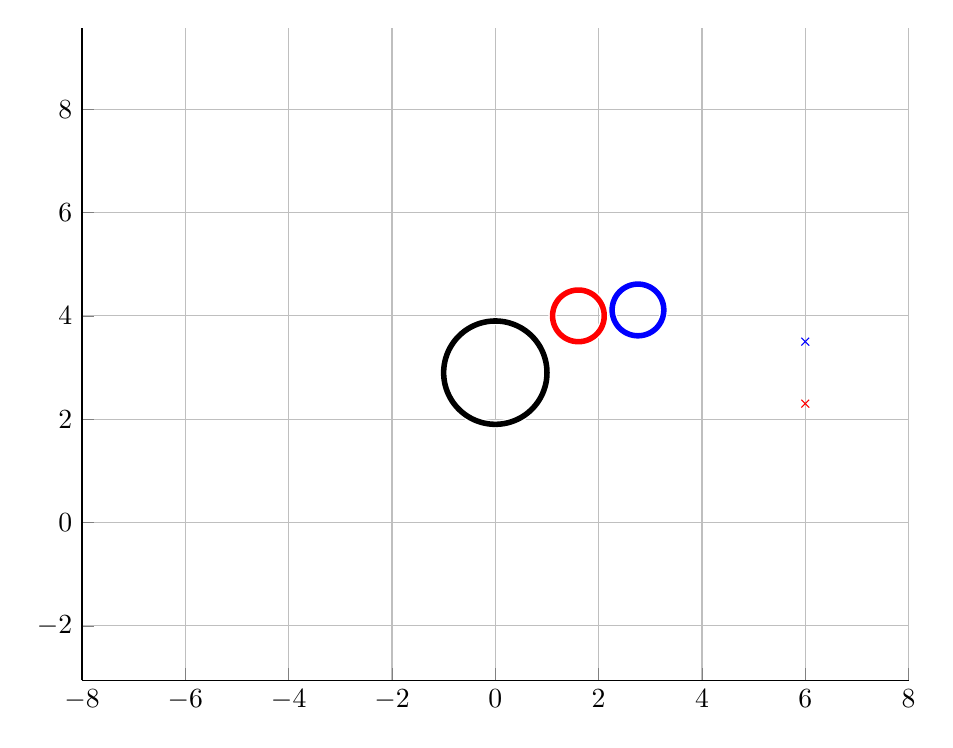
\begin{tikzpicture}

\begin{axis}[%
width=4.133in,
height=3.26in,
at={(0.693in,0.44in)},
scale only axis,
unbounded coords=jump,
xmin=-8,
xmax=8,
xmajorgrids,
ymin=-3.05283025828205,
ymax=9.56652458042763,
ymajorgrids,
axis background/.style={fill=white},
axis x line*=bottom,
axis y line*=left
]
\addplot [color=blue,only marks,mark=x,mark options={solid},forget plot]
  table[row sep=crcr]{%
6	3.5\\
};
\addplot [color=red,only marks,mark=x,mark options={solid},forget plot]
  table[row sep=crcr]{%
6	2.3\\
};
\addplot [color=white,solid,line width=3.0pt,forget plot]
  table[row sep=crcr]{%
3.26105064544558	4.11369432214559\\
3.26074605895513	4.13114407049684\\
3.25983267057549	4.14857255901765\\
3.25831159312971	4.16595855377941\\
3.25618467981636	4.18328087262562\\
3.25345452195168	4.20051841097905\\
3.25012444581248	4.21765016755447\\
3.24619850858358	4.23465526994542\\
3.24168149341474	4.25151300005408\\
3.23657890359315	4.26820281933306\\
3.23089695583853	4.28470439380842\\
3.22464257272897	4.30099761885354\\
3.21782337426688	4.31706264368349\\
3.21044766859516	4.33287989554012\\
3.20252444187504	4.34843010353853\\
3.1940633473378	4.36369432214559\\
3.18507469352379	4.37865395426219\\
3.1755694317231	4.39329077388096\\
3.16555914263305	4.40758694829182\\
3.15505602224894	4.42152505980842\\
3.14407286700507	4.43508812698886\\
3.13262305818427	4.44825962532502\\
3.1207205456149	4.46102350737508\\
3.10837983067508	4.47336422231491\\
3.09561594862501	4.48526673488428\\
3.08244445028885	4.49671654370507\\
3.06888138310841	4.50769969894895\\
3.05494327159181	4.51820281933306\\
3.04064709718095	4.52821310842311\\
3.02601027756218	4.5377183702238\\
3.01105064544558	4.54670702403781\\
2.99578642683852	4.55516811857505\\
2.98023621884012	4.56309134529517\\
2.96441896698348	4.57046705096689\\
2.94835394215353	4.57728624942898\\
2.93206071710841	4.58354063253854\\
2.91555914263305	4.58922258029316\\
2.89886932335408	4.59432517011474\\
2.88201159324541	4.59884218528358\\
2.86500649085446	4.60276812251249\\
2.84787473427904	4.60609819865169\\
2.83063719592561	4.60882835651637\\
2.8133148770794	4.61095526982972\\
2.79592888231764	4.6124763472755\\
2.77850039379683	4.61338973565513\\
2.76105064544558	4.61369432214559\\
2.74360089709433	4.61338973565513\\
2.72617240857352	4.6124763472755\\
2.70878641381175	4.61095526982972\\
2.69146409496555	4.60882835651637\\
2.67422655661211	4.60609819865169\\
2.6570948000367	4.60276812251249\\
2.64008969764574	4.59884218528358\\
2.62323196753708	4.59432517011474\\
2.6065421482581	4.58922258029316\\
2.59004057378274	4.58354063253854\\
2.57374734873762	4.57728624942898\\
2.55768232390768	4.57046705096689\\
2.54186507205104	4.56309134529517\\
2.52631486405263	4.55516811857505\\
2.51105064544558	4.54670702403781\\
2.49609101332898	4.5377183702238\\
2.4814541937102	4.52821310842311\\
2.46715801929934	4.51820281933306\\
2.45321990778275	4.50769969894895\\
2.43965684060231	4.49671654370507\\
2.42648534226615	4.48526673488428\\
2.41372146021608	4.47336422231491\\
2.40138074527625	4.46102350737508\\
2.38947823270688	4.44825962532502\\
2.37802842388609	4.43508812698886\\
2.36704526864222	4.42152505980842\\
2.3565421482581	4.40758694829182\\
2.34653185916806	4.39329077388096\\
2.33702659736736	4.37865395426219\\
2.32803794355336	4.36369432214559\\
2.31957684901611	4.34843010353853\\
2.31165362229599	4.33287989554012\\
2.30427791662428	4.31706264368349\\
2.29745871816218	4.30099761885354\\
2.29120433505262	4.28470439380842\\
2.285522387298	4.26820281933306\\
2.28041979747642	4.25151300005409\\
2.27590278230758	4.23465526994542\\
2.27197684507868	4.21765016755447\\
2.26864676893947	4.20051841097905\\
2.26591661107479	4.18328087262562\\
2.26378969776144	4.16595855377941\\
2.26226862031567	4.14857255901765\\
2.26135523193603	4.13114407049684\\
2.26105064544558	4.11369432214559\\
2.26135523193603	4.09624457379434\\
2.26226862031567	4.07881608527352\\
2.26378969776144	4.06143009051176\\
2.26591661107479	4.04410777166555\\
2.26864676893947	4.02687023331212\\
2.27197684507868	4.00973847673671\\
2.27590278230758	3.99273337434575\\
2.28041979747642	3.97587564423709\\
2.285522387298	3.95918582495811\\
2.29120433505262	3.94268425048275\\
2.29745871816218	3.92639102543763\\
2.30427791662428	3.91032600060769\\
2.31165362229599	3.89450874875105\\
2.31957684901611	3.87895854075264\\
2.32803794355336	3.86369432214559\\
2.33702659736736	3.84873469002898\\
2.34653185916806	3.83409787041021\\
2.3565421482581	3.81980169599935\\
2.36704526864222	3.80586358448276\\
2.37802842388609	3.79230051730232\\
2.38947823270688	3.77912901896616\\
2.40138074527625	3.76636513691609\\
2.41372146021608	3.75402442197626\\
2.42648534226615	3.74212190940689\\
2.43965684060231	3.7306721005861\\
2.45321990778275	3.71968894534222\\
2.46715801929934	3.70918582495811\\
2.4814541937102	3.69917553586806\\
2.49609101332898	3.68967027406737\\
2.51105064544558	3.68068162025337\\
2.52631486405263	3.67222052571612\\
2.54186507205104	3.664297298996\\
2.55768232390768	3.65692159332428\\
2.57374734873762	3.65010239486219\\
2.59004057378274	3.64384801175263\\
2.6065421482581	3.63816606399801\\
2.62323196753708	3.63306347417643\\
2.64008969764574	3.62854645900759\\
2.6570948000367	3.62462052177868\\
2.67422655661211	3.62129044563948\\
2.69146409496555	3.6185602877748\\
2.70878641381175	3.61643337446145\\
2.72617240857352	3.61491229701567\\
2.74360089709433	3.61399890863604\\
2.76105064544558	3.61369432214559\\
2.77850039379683	3.61399890863604\\
2.79592888231764	3.61491229701567\\
2.8133148770794	3.61643337446145\\
2.83063719592561	3.6185602877748\\
2.84787473427904	3.62129044563948\\
2.86500649085446	3.62462052177868\\
2.88201159324541	3.62854645900759\\
2.89886932335408	3.63306347417643\\
2.91555914263305	3.63816606399801\\
2.93206071710841	3.64384801175263\\
2.94835394215353	3.65010239486219\\
2.96441896698348	3.65692159332429\\
2.98023621884012	3.664297298996\\
2.99578642683852	3.67222052571612\\
3.01105064544558	3.68068162025337\\
3.02601027756218	3.68967027406737\\
3.04064709718095	3.69917553586806\\
3.05494327159181	3.70918582495811\\
3.06888138310841	3.71968894534222\\
3.08244445028885	3.7306721005861\\
3.09561594862501	3.74212190940689\\
3.10837983067508	3.75402442197626\\
3.1207205456149	3.76636513691609\\
3.13262305818427	3.77912901896616\\
3.14407286700507	3.79230051730232\\
3.15505602224894	3.80586358448276\\
3.16555914263305	3.81980169599935\\
3.1755694317231	3.83409787041021\\
3.18507469352379	3.84873469002898\\
3.1940633473378	3.86369432214559\\
3.20252444187504	3.87895854075264\\
3.21044766859516	3.89450874875105\\
3.21782337426688	3.91032600060769\\
3.22464257272897	3.92639102543763\\
3.23089695583853	3.94268425048275\\
3.23657890359315	3.95918582495811\\
3.24168149341474	3.97587564423709\\
3.24619850858358	3.99273337434575\\
3.25012444581248	4.00973847673671\\
3.25345452195168	4.02687023331212\\
3.25618467981636	4.04410777166555\\
3.25831159312971	4.06143009051176\\
3.25983267057549	4.07881608527352\\
3.26074605895513	4.09624457379434\\
3.26105064544558	4.11369432214559\\
nan	nan\\
};
\addplot [color=blue,solid,line width=2.0pt,forget plot]
  table[row sep=crcr]{%
3.26105064544558	4.11369432214559\\
3.26074605895513	4.13114407049684\\
3.25983267057549	4.14857255901765\\
3.25831159312971	4.16595855377941\\
3.25618467981636	4.18328087262562\\
3.25345452195168	4.20051841097905\\
3.25012444581248	4.21765016755447\\
3.24619850858358	4.23465526994542\\
3.24168149341474	4.25151300005408\\
3.23657890359315	4.26820281933306\\
3.23089695583853	4.28470439380842\\
3.22464257272897	4.30099761885354\\
3.21782337426688	4.31706264368349\\
3.21044766859516	4.33287989554012\\
3.20252444187504	4.34843010353853\\
3.1940633473378	4.36369432214559\\
3.18507469352379	4.37865395426219\\
3.1755694317231	4.39329077388096\\
3.16555914263305	4.40758694829182\\
3.15505602224894	4.42152505980842\\
3.14407286700507	4.43508812698886\\
3.13262305818427	4.44825962532502\\
3.1207205456149	4.46102350737508\\
3.10837983067508	4.47336422231491\\
3.09561594862501	4.48526673488428\\
3.08244445028885	4.49671654370507\\
3.06888138310841	4.50769969894895\\
3.05494327159181	4.51820281933306\\
3.04064709718095	4.52821310842311\\
3.02601027756218	4.5377183702238\\
3.01105064544558	4.54670702403781\\
2.99578642683852	4.55516811857505\\
2.98023621884012	4.56309134529517\\
2.96441896698348	4.57046705096689\\
2.94835394215353	4.57728624942898\\
2.93206071710841	4.58354063253854\\
2.91555914263305	4.58922258029316\\
2.89886932335408	4.59432517011474\\
2.88201159324541	4.59884218528358\\
2.86500649085446	4.60276812251249\\
2.84787473427904	4.60609819865169\\
2.83063719592561	4.60882835651637\\
2.8133148770794	4.61095526982972\\
2.79592888231764	4.6124763472755\\
2.77850039379683	4.61338973565513\\
2.76105064544558	4.61369432214559\\
2.74360089709433	4.61338973565513\\
2.72617240857352	4.6124763472755\\
2.70878641381175	4.61095526982972\\
2.69146409496555	4.60882835651637\\
2.67422655661211	4.60609819865169\\
2.6570948000367	4.60276812251249\\
2.64008969764574	4.59884218528358\\
2.62323196753708	4.59432517011474\\
2.6065421482581	4.58922258029316\\
2.59004057378274	4.58354063253854\\
2.57374734873762	4.57728624942898\\
2.55768232390768	4.57046705096689\\
2.54186507205104	4.56309134529517\\
2.52631486405263	4.55516811857505\\
2.51105064544558	4.54670702403781\\
2.49609101332898	4.5377183702238\\
2.4814541937102	4.52821310842311\\
2.46715801929934	4.51820281933306\\
2.45321990778275	4.50769969894895\\
2.43965684060231	4.49671654370507\\
2.42648534226615	4.48526673488428\\
2.41372146021608	4.47336422231491\\
2.40138074527625	4.46102350737508\\
2.38947823270688	4.44825962532502\\
2.37802842388609	4.43508812698886\\
2.36704526864222	4.42152505980842\\
2.3565421482581	4.40758694829182\\
2.34653185916806	4.39329077388096\\
2.33702659736736	4.37865395426219\\
2.32803794355336	4.36369432214559\\
2.31957684901611	4.34843010353853\\
2.31165362229599	4.33287989554012\\
2.30427791662428	4.31706264368349\\
2.29745871816218	4.30099761885354\\
2.29120433505262	4.28470439380842\\
2.285522387298	4.26820281933306\\
2.28041979747642	4.25151300005409\\
2.27590278230758	4.23465526994542\\
2.27197684507868	4.21765016755447\\
2.26864676893947	4.20051841097905\\
2.26591661107479	4.18328087262562\\
2.26378969776144	4.16595855377941\\
2.26226862031567	4.14857255901765\\
2.26135523193603	4.13114407049684\\
2.26105064544558	4.11369432214559\\
2.26135523193603	4.09624457379434\\
2.26226862031567	4.07881608527352\\
2.26378969776144	4.06143009051176\\
2.26591661107479	4.04410777166555\\
2.26864676893947	4.02687023331212\\
2.27197684507868	4.00973847673671\\
2.27590278230758	3.99273337434575\\
2.28041979747642	3.97587564423709\\
2.285522387298	3.95918582495811\\
2.29120433505262	3.94268425048275\\
2.29745871816218	3.92639102543763\\
2.30427791662428	3.91032600060769\\
2.31165362229599	3.89450874875105\\
2.31957684901611	3.87895854075264\\
2.32803794355336	3.86369432214559\\
2.33702659736736	3.84873469002898\\
2.34653185916806	3.83409787041021\\
2.3565421482581	3.81980169599935\\
2.36704526864222	3.80586358448276\\
2.37802842388609	3.79230051730232\\
2.38947823270688	3.77912901896616\\
2.40138074527625	3.76636513691609\\
2.41372146021608	3.75402442197626\\
2.42648534226615	3.74212190940689\\
2.43965684060231	3.7306721005861\\
2.45321990778275	3.71968894534222\\
2.46715801929934	3.70918582495811\\
2.4814541937102	3.69917553586806\\
2.49609101332898	3.68967027406737\\
2.51105064544558	3.68068162025337\\
2.52631486405263	3.67222052571612\\
2.54186507205104	3.664297298996\\
2.55768232390768	3.65692159332428\\
2.57374734873762	3.65010239486219\\
2.59004057378274	3.64384801175263\\
2.6065421482581	3.63816606399801\\
2.62323196753708	3.63306347417643\\
2.64008969764574	3.62854645900759\\
2.6570948000367	3.62462052177868\\
2.67422655661211	3.62129044563948\\
2.69146409496555	3.6185602877748\\
2.70878641381175	3.61643337446145\\
2.72617240857352	3.61491229701567\\
2.74360089709433	3.61399890863604\\
2.76105064544558	3.61369432214559\\
2.77850039379683	3.61399890863604\\
2.79592888231764	3.61491229701567\\
2.8133148770794	3.61643337446145\\
2.83063719592561	3.6185602877748\\
2.84787473427904	3.62129044563948\\
2.86500649085446	3.62462052177868\\
2.88201159324541	3.62854645900759\\
2.89886932335408	3.63306347417643\\
2.91555914263305	3.63816606399801\\
2.93206071710841	3.64384801175263\\
2.94835394215353	3.65010239486219\\
2.96441896698348	3.65692159332429\\
2.98023621884012	3.664297298996\\
2.99578642683852	3.67222052571612\\
3.01105064544558	3.68068162025337\\
3.02601027756218	3.68967027406737\\
3.04064709718095	3.69917553586806\\
3.05494327159181	3.70918582495811\\
3.06888138310841	3.71968894534222\\
3.08244445028885	3.7306721005861\\
3.09561594862501	3.74212190940689\\
3.10837983067508	3.75402442197626\\
3.1207205456149	3.76636513691609\\
3.13262305818427	3.77912901896616\\
3.14407286700507	3.79230051730232\\
3.15505602224894	3.80586358448276\\
3.16555914263305	3.81980169599935\\
3.1755694317231	3.83409787041021\\
3.18507469352379	3.84873469002898\\
3.1940633473378	3.86369432214559\\
3.20252444187504	3.87895854075264\\
3.21044766859516	3.89450874875105\\
3.21782337426688	3.91032600060769\\
3.22464257272897	3.92639102543763\\
3.23089695583853	3.94268425048275\\
3.23657890359315	3.95918582495811\\
3.24168149341474	3.97587564423709\\
3.24619850858358	3.99273337434575\\
3.25012444581248	4.00973847673671\\
3.25345452195168	4.02687023331212\\
3.25618467981636	4.04410777166555\\
3.25831159312971	4.06143009051176\\
3.25983267057549	4.07881608527352\\
3.26074605895513	4.09624457379434\\
3.26105064544558	4.11369432214559\\
nan	nan\\
};
\addplot [color=white,solid,line width=3.0pt,forget plot]
  table[row sep=crcr]{%
2.10804355233902	3.99928625125649\\
2.10773896584857	4.01673599960774\\
2.10682557746893	4.03416448812856\\
2.10530450002316	4.05155048289032\\
2.1031775867098	4.06887280173653\\
2.10044742884512	4.08611034008996\\
2.09711735270592	4.10324209666537\\
2.09319141547702	4.12024719905633\\
2.08867440030818	4.13710492916499\\
2.0835718104866	4.15379474844397\\
2.07788986273197	4.17029632291933\\
2.07163547962241	4.18658954796445\\
2.06481628116032	4.20265457279439\\
2.0574405754886	4.21847182465103\\
2.04951734876848	4.23402203264944\\
2.04105625423124	4.24928625125649\\
2.03206760041723	4.2642458833731\\
2.02256233861654	4.27888270299187\\
2.01255204952649	4.29317887740273\\
2.00204892914238	4.30711698891932\\
1.99106577389851	4.32068005609976\\
1.97961596507772	4.33385155443592\\
1.96771345250834	4.34661543648599\\
1.95537273756852	4.35895615142582\\
1.94260885551845	4.37085866399519\\
1.92943735718229	4.38230847281598\\
1.91587429000185	4.39329162805985\\
1.90193617848526	4.40379474844397\\
1.88764000407439	4.41380503753401\\
1.87300318445562	4.42331029933471\\
1.85804355233902	4.43229895314871\\
1.84277933373196	4.44076004768596\\
1.82722912573356	4.44868327440608\\
1.81141187387692	4.45605898007779\\
1.79534684904697	4.46287817853989\\
1.77905362400185	4.46913256164945\\
1.76255204952649	4.47481450940407\\
1.74586223024752	4.47991709922565\\
1.72900450013885	4.48443411439449\\
1.7119993977479	4.4883600516234\\
1.69486764117248	4.4916901277626\\
1.67763010281905	4.49442028562728\\
1.66030778397285	4.49654719894063\\
1.64292178921108	4.49806827638641\\
1.62549330069027	4.49898166476604\\
1.60804355233902	4.49928625125649\\
1.59059380398777	4.49898166476604\\
1.57316531546696	4.49806827638641\\
1.55577932070519	4.49654719894063\\
1.53845700185899	4.49442028562728\\
1.52121946350555	4.4916901277626\\
1.50408770693014	4.4883600516234\\
1.48708260453918	4.48443411439449\\
1.47022487443052	4.47991709922565\\
1.45353505515154	4.47481450940407\\
1.43703348067618	4.46913256164945\\
1.42074025563106	4.46287817853989\\
1.40467523080112	4.45605898007779\\
1.38885797894448	4.44868327440608\\
1.37330777094607	4.44076004768596\\
1.35804355233902	4.43229895314871\\
1.34308392022242	4.42331029933471\\
1.32844710060365	4.41380503753401\\
1.31415092619278	4.40379474844397\\
1.30021281467619	4.39329162805985\\
1.28664974749575	4.38230847281598\\
1.27347824915959	4.37085866399519\\
1.26071436710952	4.35895615142582\\
1.24837365216969	4.34661543648599\\
1.23647113960032	4.33385155443592\\
1.22502133077953	4.32068005609976\\
1.21403817553566	4.30711698891932\\
1.20353505515154	4.29317887740273\\
1.1935247660615	4.27888270299187\\
1.18401950426081	4.2642458833731\\
1.1750308504468	4.24928625125649\\
1.16656975590955	4.23402203264944\\
1.15864652918944	4.21847182465103\\
1.15127082351772	4.20265457279439\\
1.14445162505562	4.18658954796445\\
1.13819724194606	4.17029632291933\\
1.13251529419144	4.15379474844397\\
1.12741270436986	4.13710492916499\\
1.12289568920102	4.12024719905633\\
1.11896975197212	4.10324209666537\\
1.11563967583291	4.08611034008996\\
1.11290951796823	4.06887280173653\\
1.11078260465488	4.05155048289032\\
1.10926152720911	4.03416448812856\\
1.10834813882947	4.01673599960774\\
1.10804355233902	3.99928625125649\\
1.10834813882947	3.98183650290524\\
1.10926152720911	3.96440801438443\\
1.11078260465488	3.94702201962267\\
1.11290951796823	3.92969970077646\\
1.11563967583291	3.91246216242303\\
1.11896975197212	3.89533040584761\\
1.12289568920102	3.87832530345666\\
1.12741270436986	3.86146757334799\\
1.13251529419144	3.84477775406902\\
1.13819724194606	3.82827617959366\\
1.14445162505562	3.81198295454854\\
1.15127082351772	3.79591792971859\\
1.15864652918943	3.78010067786195\\
1.16656975590955	3.76455046986355\\
1.1750308504468	3.74928625125649\\
1.18401950426081	3.73432661913989\\
1.1935247660615	3.71968979952112\\
1.20353505515154	3.70539362511026\\
1.21403817553566	3.69145551359366\\
1.22502133077953	3.67789244641322\\
1.23647113960032	3.66472094807706\\
1.24837365216969	3.65195706602699\\
1.26071436710952	3.63961635108717\\
1.27347824915959	3.6277138385178\\
1.28664974749575	3.616264029697\\
1.30021281467619	3.60528087445313\\
1.31415092619278	3.59477775406902\\
1.32844710060364	3.58476746497897\\
1.34308392022242	3.57526220317828\\
1.35804355233902	3.56627354936427\\
1.37330777094607	3.55781245482703\\
1.38885797894448	3.54988922810691\\
1.40467523080112	3.54251352243519\\
1.42074025563106	3.5356943239731\\
1.43703348067618	3.52943994086354\\
1.45353505515154	3.52375799310892\\
1.47022487443052	3.51865540328733\\
1.48708260453918	3.51413838811849\\
1.50408770693014	3.51021245088959\\
1.52121946350555	3.50688237475039\\
1.53845700185899	3.50415221688571\\
1.55577932070519	3.50202530357236\\
1.57316531546696	3.50050422612658\\
1.59059380398777	3.49959083774695\\
1.60804355233902	3.49928625125649\\
1.62549330069027	3.49959083774695\\
1.64292178921108	3.50050422612658\\
1.66030778397284	3.50202530357236\\
1.67763010281905	3.50415221688571\\
1.69486764117248	3.50688237475039\\
1.7119993977479	3.51021245088959\\
1.72900450013885	3.51413838811849\\
1.74586223024752	3.51865540328733\\
1.76255204952649	3.52375799310892\\
1.77905362400185	3.52943994086354\\
1.79534684904697	3.5356943239731\\
1.81141187387692	3.54251352243519\\
1.82722912573356	3.54988922810691\\
1.84277933373196	3.55781245482703\\
1.85804355233902	3.56627354936427\\
1.87300318445562	3.57526220317828\\
1.88764000407439	3.58476746497897\\
1.90193617848525	3.59477775406902\\
1.91587429000185	3.60528087445313\\
1.92943735718229	3.616264029697\\
1.94260885551845	3.6277138385178\\
1.95537273756852	3.63961635108717\\
1.96771345250834	3.65195706602699\\
1.97961596507772	3.66472094807706\\
1.99106577389851	3.67789244641322\\
2.00204892914238	3.69145551359366\\
2.01255204952649	3.70539362511026\\
2.02256233861654	3.71968979952112\\
2.03206760041723	3.73432661913989\\
2.04105625423124	3.74928625125649\\
2.04951734876848	3.76455046986355\\
2.0574405754886	3.78010067786195\\
2.06481628116032	3.79591792971859\\
2.07163547962241	3.81198295454854\\
2.07788986273197	3.82827617959366\\
2.0835718104866	3.84477775406902\\
2.08867440030818	3.86146757334799\\
2.09319141547702	3.87832530345666\\
2.09711735270592	3.89533040584761\\
2.10044742884512	3.91246216242303\\
2.1031775867098	3.92969970077646\\
2.10530450002316	3.94702201962267\\
2.10682557746893	3.96440801438443\\
2.10773896584857	3.98183650290524\\
2.10804355233902	3.99928625125649\\
nan	nan\\
};
\addplot [color=red,solid,line width=2.0pt,forget plot]
  table[row sep=crcr]{%
2.10804355233902	3.99928625125649\\
2.10773896584857	4.01673599960774\\
2.10682557746893	4.03416448812856\\
2.10530450002316	4.05155048289032\\
2.1031775867098	4.06887280173653\\
2.10044742884512	4.08611034008996\\
2.09711735270592	4.10324209666537\\
2.09319141547702	4.12024719905633\\
2.08867440030818	4.13710492916499\\
2.0835718104866	4.15379474844397\\
2.07788986273197	4.17029632291933\\
2.07163547962241	4.18658954796445\\
2.06481628116032	4.20265457279439\\
2.0574405754886	4.21847182465103\\
2.04951734876848	4.23402203264944\\
2.04105625423124	4.24928625125649\\
2.03206760041723	4.2642458833731\\
2.02256233861654	4.27888270299187\\
2.01255204952649	4.29317887740273\\
2.00204892914238	4.30711698891932\\
1.99106577389851	4.32068005609976\\
1.97961596507772	4.33385155443592\\
1.96771345250834	4.34661543648599\\
1.95537273756852	4.35895615142582\\
1.94260885551845	4.37085866399519\\
1.92943735718229	4.38230847281598\\
1.91587429000185	4.39329162805985\\
1.90193617848526	4.40379474844397\\
1.88764000407439	4.41380503753401\\
1.87300318445562	4.42331029933471\\
1.85804355233902	4.43229895314871\\
1.84277933373196	4.44076004768596\\
1.82722912573356	4.44868327440608\\
1.81141187387692	4.45605898007779\\
1.79534684904697	4.46287817853989\\
1.77905362400185	4.46913256164945\\
1.76255204952649	4.47481450940407\\
1.74586223024752	4.47991709922565\\
1.72900450013885	4.48443411439449\\
1.7119993977479	4.4883600516234\\
1.69486764117248	4.4916901277626\\
1.67763010281905	4.49442028562728\\
1.66030778397285	4.49654719894063\\
1.64292178921108	4.49806827638641\\
1.62549330069027	4.49898166476604\\
1.60804355233902	4.49928625125649\\
1.59059380398777	4.49898166476604\\
1.57316531546696	4.49806827638641\\
1.55577932070519	4.49654719894063\\
1.53845700185899	4.49442028562728\\
1.52121946350555	4.4916901277626\\
1.50408770693014	4.4883600516234\\
1.48708260453918	4.48443411439449\\
1.47022487443052	4.47991709922565\\
1.45353505515154	4.47481450940407\\
1.43703348067618	4.46913256164945\\
1.42074025563106	4.46287817853989\\
1.40467523080112	4.45605898007779\\
1.38885797894448	4.44868327440608\\
1.37330777094607	4.44076004768596\\
1.35804355233902	4.43229895314871\\
1.34308392022242	4.42331029933471\\
1.32844710060365	4.41380503753401\\
1.31415092619278	4.40379474844397\\
1.30021281467619	4.39329162805985\\
1.28664974749575	4.38230847281598\\
1.27347824915959	4.37085866399519\\
1.26071436710952	4.35895615142582\\
1.24837365216969	4.34661543648599\\
1.23647113960032	4.33385155443592\\
1.22502133077953	4.32068005609976\\
1.21403817553566	4.30711698891932\\
1.20353505515154	4.29317887740273\\
1.1935247660615	4.27888270299187\\
1.18401950426081	4.2642458833731\\
1.1750308504468	4.24928625125649\\
1.16656975590955	4.23402203264944\\
1.15864652918944	4.21847182465103\\
1.15127082351772	4.20265457279439\\
1.14445162505562	4.18658954796445\\
1.13819724194606	4.17029632291933\\
1.13251529419144	4.15379474844397\\
1.12741270436986	4.13710492916499\\
1.12289568920102	4.12024719905633\\
1.11896975197212	4.10324209666537\\
1.11563967583291	4.08611034008996\\
1.11290951796823	4.06887280173653\\
1.11078260465488	4.05155048289032\\
1.10926152720911	4.03416448812856\\
1.10834813882947	4.01673599960774\\
1.10804355233902	3.99928625125649\\
1.10834813882947	3.98183650290524\\
1.10926152720911	3.96440801438443\\
1.11078260465488	3.94702201962267\\
1.11290951796823	3.92969970077646\\
1.11563967583291	3.91246216242303\\
1.11896975197212	3.89533040584761\\
1.12289568920102	3.87832530345666\\
1.12741270436986	3.86146757334799\\
1.13251529419144	3.84477775406902\\
1.13819724194606	3.82827617959366\\
1.14445162505562	3.81198295454854\\
1.15127082351772	3.79591792971859\\
1.15864652918943	3.78010067786195\\
1.16656975590955	3.76455046986355\\
1.1750308504468	3.74928625125649\\
1.18401950426081	3.73432661913989\\
1.1935247660615	3.71968979952112\\
1.20353505515154	3.70539362511026\\
1.21403817553566	3.69145551359366\\
1.22502133077953	3.67789244641322\\
1.23647113960032	3.66472094807706\\
1.24837365216969	3.65195706602699\\
1.26071436710952	3.63961635108717\\
1.27347824915959	3.6277138385178\\
1.28664974749575	3.616264029697\\
1.30021281467619	3.60528087445313\\
1.31415092619278	3.59477775406902\\
1.32844710060364	3.58476746497897\\
1.34308392022242	3.57526220317828\\
1.35804355233902	3.56627354936427\\
1.37330777094607	3.55781245482703\\
1.38885797894448	3.54988922810691\\
1.40467523080112	3.54251352243519\\
1.42074025563106	3.5356943239731\\
1.43703348067618	3.52943994086354\\
1.45353505515154	3.52375799310892\\
1.47022487443052	3.51865540328733\\
1.48708260453918	3.51413838811849\\
1.50408770693014	3.51021245088959\\
1.52121946350555	3.50688237475039\\
1.53845700185899	3.50415221688571\\
1.55577932070519	3.50202530357236\\
1.57316531546696	3.50050422612658\\
1.59059380398777	3.49959083774695\\
1.60804355233902	3.49928625125649\\
1.62549330069027	3.49959083774695\\
1.64292178921108	3.50050422612658\\
1.66030778397284	3.50202530357236\\
1.67763010281905	3.50415221688571\\
1.69486764117248	3.50688237475039\\
1.7119993977479	3.51021245088959\\
1.72900450013885	3.51413838811849\\
1.74586223024752	3.51865540328733\\
1.76255204952649	3.52375799310892\\
1.77905362400185	3.52943994086354\\
1.79534684904697	3.5356943239731\\
1.81141187387692	3.54251352243519\\
1.82722912573356	3.54988922810691\\
1.84277933373196	3.55781245482703\\
1.85804355233902	3.56627354936427\\
1.87300318445562	3.57526220317828\\
1.88764000407439	3.58476746497897\\
1.90193617848525	3.59477775406902\\
1.91587429000185	3.60528087445313\\
1.92943735718229	3.616264029697\\
1.94260885551845	3.6277138385178\\
1.95537273756852	3.63961635108717\\
1.96771345250834	3.65195706602699\\
1.97961596507772	3.66472094807706\\
1.99106577389851	3.67789244641322\\
2.00204892914238	3.69145551359366\\
2.01255204952649	3.70539362511026\\
2.02256233861654	3.71968979952112\\
2.03206760041723	3.73432661913989\\
2.04105625423124	3.74928625125649\\
2.04951734876848	3.76455046986355\\
2.0574405754886	3.78010067786195\\
2.06481628116032	3.79591792971859\\
2.07163547962241	3.81198295454854\\
2.07788986273197	3.82827617959366\\
2.0835718104866	3.84477775406902\\
2.08867440030818	3.86146757334799\\
2.09319141547702	3.87832530345666\\
2.09711735270592	3.89533040584761\\
2.10044742884512	3.91246216242303\\
2.1031775867098	3.92969970077646\\
2.10530450002316	3.94702201962267\\
2.10682557746893	3.96440801438443\\
2.10773896584857	3.98183650290524\\
2.10804355233902	3.99928625125649\\
nan	nan\\
};
\addplot [color=white,solid,line width=3.0pt,forget plot]
  table[row sep=crcr]{%
1	2.9\\
0.999390827019096	2.9348994967025\\
0.997564050259824	2.96975647374413\\
0.994521895368273	3.00452846326765\\
0.99026806874157	3.03917310096007\\
0.984807753012208	3.07364817766693\\
0.978147600733806	3.10791169081776\\
0.970295726275996	3.14192189559967\\
0.961261695938319	3.175637355817\\
0.951056516295154	3.20901699437495\\
0.939692620785908	3.24202014332567\\
0.927183854566787	3.27460659341591\\
0.913545457642601	3.3067366430758\\
0.898794046299167	3.33837114678908\\
0.882947592858927	3.36947156278589\\
0.866025403784439	3.4\\
0.848048096156426	3.42991926423321\\
0.829037572555042	3.45919290347075\\
0.809016994374947	3.48778525229247\\
0.788010753606722	3.51566147532566\\
0.766044443118978	3.54278760968654\\
0.743144825477394	3.56913060635886\\
0.719339800338651	3.594658370459\\
0.694658370458997	3.61933980033865\\
0.669130606358858	3.64314482547739\\
0.642787609686539	3.66604444311898\\
0.615661475325658	3.68801075360672\\
0.587785252292473	3.70901699437495\\
0.559192903470747	3.72903757255504\\
0.529919264233205	3.74804809615643\\
0.5	3.76602540378444\\
0.469471562785891	3.78294759285893\\
0.438371146789077	3.79879404629917\\
0.4067366430758	3.8135454576426\\
0.374606593415912	3.82718385456679\\
0.342020143325669	3.83969262078591\\
0.309016994374947	3.85105651629515\\
0.275637355816999	3.86126169593832\\
0.241921895599668	3.870295726276\\
0.207911690817759	3.87814760073381\\
0.17364817766693	3.88480775301221\\
0.139173100960066	3.89026806874157\\
0.104528463267653	3.89452189536827\\
0.0697564737441255	3.89756405025982\\
0.0348994967025011	3.8993908270191\\
6.12323399573677e-17	3.9\\
-0.0348994967025007	3.8993908270191\\
-0.0697564737441253	3.89756405025982\\
-0.104528463267653	3.89452189536827\\
-0.139173100960065	3.89026806874157\\
-0.17364817766693	3.88480775301221\\
-0.207911690817759	3.87814760073381\\
-0.241921895599668	3.870295726276\\
-0.275637355816999	3.86126169593832\\
-0.309016994374947	3.85105651629515\\
-0.342020143325669	3.83969262078591\\
-0.374606593415912	3.82718385456679\\
-0.4067366430758	3.8135454576426\\
-0.438371146789078	3.79879404629917\\
-0.469471562785891	3.78294759285893\\
-0.5	3.76602540378444\\
-0.529919264233205	3.74804809615643\\
-0.559192903470747	3.72903757255504\\
-0.587785252292473	3.70901699437495\\
-0.615661475325658	3.68801075360672\\
-0.642787609686539	3.66604444311898\\
-0.669130606358858	3.64314482547739\\
-0.694658370458997	3.61933980033865\\
-0.719339800338651	3.594658370459\\
-0.743144825477394	3.56913060635886\\
-0.766044443118978	3.54278760968654\\
-0.788010753606722	3.51566147532566\\
-0.809016994374947	3.48778525229247\\
-0.829037572555042	3.45919290347075\\
-0.848048096156426	3.42991926423321\\
-0.866025403784439	3.4\\
-0.882947592858927	3.36947156278589\\
-0.898794046299167	3.33837114678908\\
-0.913545457642601	3.3067366430758\\
-0.927183854566787	3.27460659341591\\
-0.939692620785908	3.24202014332567\\
-0.951056516295154	3.20901699437495\\
-0.961261695938319	3.175637355817\\
-0.970295726275996	3.14192189559967\\
-0.978147600733806	3.10791169081776\\
-0.984807753012208	3.07364817766693\\
-0.99026806874157	3.03917310096007\\
-0.994521895368273	3.00452846326765\\
-0.997564050259824	2.96975647374413\\
-0.999390827019096	2.9348994967025\\
-1	2.9\\
-0.999390827019096	2.8651005032975\\
-0.997564050259824	2.83024352625588\\
-0.994521895368273	2.79547153673235\\
-0.99026806874157	2.76082689903993\\
-0.984807753012208	2.72635182233307\\
-0.978147600733806	2.69208830918224\\
-0.970295726275997	2.65807810440033\\
-0.961261695938319	2.624362644183\\
-0.951056516295154	2.59098300562505\\
-0.939692620785908	2.55797985667433\\
-0.927183854566787	2.52539340658409\\
-0.913545457642601	2.4932633569242\\
-0.898794046299167	2.46162885321092\\
-0.882947592858927	2.43052843721411\\
-0.866025403784439	2.4\\
-0.848048096156426	2.3700807357668\\
-0.829037572555042	2.34080709652925\\
-0.809016994374947	2.31221474770753\\
-0.788010753606722	2.28433852467434\\
-0.766044443118978	2.25721239031346\\
-0.743144825477394	2.23086939364114\\
-0.719339800338651	2.205341629541\\
-0.694658370458997	2.18066019966135\\
-0.669130606358858	2.15685517452261\\
-0.642787609686539	2.13395555688102\\
-0.615661475325658	2.11198924639328\\
-0.587785252292473	2.09098300562505\\
-0.559192903470747	2.07096242744496\\
-0.529919264233205	2.05195190384357\\
-0.5	2.03397459621556\\
-0.469471562785891	2.01705240714107\\
-0.438371146789078	2.00120595370083\\
-0.4067366430758	1.9864545423574\\
-0.374606593415912	1.97281614543321\\
-0.342020143325669	1.96030737921409\\
-0.309016994374948	1.94894348370485\\
-0.275637355816999	1.93873830406168\\
-0.241921895599668	1.929704273724\\
-0.20791169081776	1.92185239926619\\
-0.17364817766693	1.91519224698779\\
-0.139173100960065	1.90973193125843\\
-0.104528463267653	1.90547810463173\\
-0.0697564737441256	1.90243594974018\\
-0.0348994967025016	1.9006091729809\\
-1.83697019872103e-16	1.9\\
0.0348994967025013	1.9006091729809\\
0.0697564737441252	1.90243594974018\\
0.104528463267653	1.90547810463173\\
0.139173100960065	1.90973193125843\\
0.17364817766693	1.91519224698779\\
0.207911690817759	1.92185239926619\\
0.241921895599667	1.929704273724\\
0.275637355816999	1.93873830406168\\
0.309016994374947	1.94894348370485\\
0.342020143325668	1.96030737921409\\
0.374606593415912	1.97281614543321\\
0.406736643075801	1.9864545423574\\
0.438371146789077	2.00120595370083\\
0.46947156278589	2.01705240714107\\
0.5	2.03397459621556\\
0.529919264233205	2.05195190384357\\
0.559192903470746	2.07096242744496\\
0.587785252292473	2.09098300562505\\
0.615661475325659	2.11198924639328\\
0.642787609686539	2.13395555688102\\
0.669130606358858	2.15685517452261\\
0.694658370458997	2.18066019966135\\
0.719339800338651	2.205341629541\\
0.743144825477394	2.23086939364114\\
0.766044443118978	2.25721239031346\\
0.788010753606722	2.28433852467434\\
0.809016994374947	2.31221474770753\\
0.829037572555041	2.34080709652925\\
0.848048096156425	2.37008073576679\\
0.866025403784438	2.4\\
0.882947592858927	2.43052843721411\\
0.898794046299167	2.46162885321092\\
0.913545457642601	2.4932633569242\\
0.927183854566787	2.52539340658409\\
0.939692620785908	2.55797985667433\\
0.951056516295154	2.59098300562505\\
0.961261695938319	2.624362644183\\
0.970295726275996	2.65807810440033\\
0.978147600733806	2.69208830918224\\
0.984807753012208	2.72635182233307\\
0.99026806874157	2.76082689903993\\
0.994521895368273	2.79547153673235\\
0.997564050259824	2.83024352625588\\
0.999390827019096	2.8651005032975\\
1	2.9\\
nan	nan\\
};
\addplot [color=black,solid,line width=2.0pt,forget plot]
  table[row sep=crcr]{%
1	2.9\\
0.999390827019096	2.9348994967025\\
0.997564050259824	2.96975647374413\\
0.994521895368273	3.00452846326765\\
0.99026806874157	3.03917310096007\\
0.984807753012208	3.07364817766693\\
0.978147600733806	3.10791169081776\\
0.970295726275996	3.14192189559967\\
0.961261695938319	3.175637355817\\
0.951056516295154	3.20901699437495\\
0.939692620785908	3.24202014332567\\
0.927183854566787	3.27460659341591\\
0.913545457642601	3.3067366430758\\
0.898794046299167	3.33837114678908\\
0.882947592858927	3.36947156278589\\
0.866025403784439	3.4\\
0.848048096156426	3.42991926423321\\
0.829037572555042	3.45919290347075\\
0.809016994374947	3.48778525229247\\
0.788010753606722	3.51566147532566\\
0.766044443118978	3.54278760968654\\
0.743144825477394	3.56913060635886\\
0.719339800338651	3.594658370459\\
0.694658370458997	3.61933980033865\\
0.669130606358858	3.64314482547739\\
0.642787609686539	3.66604444311898\\
0.615661475325658	3.68801075360672\\
0.587785252292473	3.70901699437495\\
0.559192903470747	3.72903757255504\\
0.529919264233205	3.74804809615643\\
0.5	3.76602540378444\\
0.469471562785891	3.78294759285893\\
0.438371146789077	3.79879404629917\\
0.4067366430758	3.8135454576426\\
0.374606593415912	3.82718385456679\\
0.342020143325669	3.83969262078591\\
0.309016994374947	3.85105651629515\\
0.275637355816999	3.86126169593832\\
0.241921895599668	3.870295726276\\
0.207911690817759	3.87814760073381\\
0.17364817766693	3.88480775301221\\
0.139173100960066	3.89026806874157\\
0.104528463267653	3.89452189536827\\
0.0697564737441255	3.89756405025982\\
0.0348994967025011	3.8993908270191\\
6.12323399573677e-17	3.9\\
-0.0348994967025007	3.8993908270191\\
-0.0697564737441253	3.89756405025982\\
-0.104528463267653	3.89452189536827\\
-0.139173100960065	3.89026806874157\\
-0.17364817766693	3.88480775301221\\
-0.207911690817759	3.87814760073381\\
-0.241921895599668	3.870295726276\\
-0.275637355816999	3.86126169593832\\
-0.309016994374947	3.85105651629515\\
-0.342020143325669	3.83969262078591\\
-0.374606593415912	3.82718385456679\\
-0.4067366430758	3.8135454576426\\
-0.438371146789078	3.79879404629917\\
-0.469471562785891	3.78294759285893\\
-0.5	3.76602540378444\\
-0.529919264233205	3.74804809615643\\
-0.559192903470747	3.72903757255504\\
-0.587785252292473	3.70901699437495\\
-0.615661475325658	3.68801075360672\\
-0.642787609686539	3.66604444311898\\
-0.669130606358858	3.64314482547739\\
-0.694658370458997	3.61933980033865\\
-0.719339800338651	3.594658370459\\
-0.743144825477394	3.56913060635886\\
-0.766044443118978	3.54278760968654\\
-0.788010753606722	3.51566147532566\\
-0.809016994374947	3.48778525229247\\
-0.829037572555042	3.45919290347075\\
-0.848048096156426	3.42991926423321\\
-0.866025403784439	3.4\\
-0.882947592858927	3.36947156278589\\
-0.898794046299167	3.33837114678908\\
-0.913545457642601	3.3067366430758\\
-0.927183854566787	3.27460659341591\\
-0.939692620785908	3.24202014332567\\
-0.951056516295154	3.20901699437495\\
-0.961261695938319	3.175637355817\\
-0.970295726275996	3.14192189559967\\
-0.978147600733806	3.10791169081776\\
-0.984807753012208	3.07364817766693\\
-0.99026806874157	3.03917310096007\\
-0.994521895368273	3.00452846326765\\
-0.997564050259824	2.96975647374413\\
-0.999390827019096	2.9348994967025\\
-1	2.9\\
-0.999390827019096	2.8651005032975\\
-0.997564050259824	2.83024352625588\\
-0.994521895368273	2.79547153673235\\
-0.99026806874157	2.76082689903993\\
-0.984807753012208	2.72635182233307\\
-0.978147600733806	2.69208830918224\\
-0.970295726275997	2.65807810440033\\
-0.961261695938319	2.624362644183\\
-0.951056516295154	2.59098300562505\\
-0.939692620785908	2.55797985667433\\
-0.927183854566787	2.52539340658409\\
-0.913545457642601	2.4932633569242\\
-0.898794046299167	2.46162885321092\\
-0.882947592858927	2.43052843721411\\
-0.866025403784439	2.4\\
-0.848048096156426	2.3700807357668\\
-0.829037572555042	2.34080709652925\\
-0.809016994374947	2.31221474770753\\
-0.788010753606722	2.28433852467434\\
-0.766044443118978	2.25721239031346\\
-0.743144825477394	2.23086939364114\\
-0.719339800338651	2.205341629541\\
-0.694658370458997	2.18066019966135\\
-0.669130606358858	2.15685517452261\\
-0.642787609686539	2.13395555688102\\
-0.615661475325658	2.11198924639328\\
-0.587785252292473	2.09098300562505\\
-0.559192903470747	2.07096242744496\\
-0.529919264233205	2.05195190384357\\
-0.5	2.03397459621556\\
-0.469471562785891	2.01705240714107\\
-0.438371146789078	2.00120595370083\\
-0.4067366430758	1.9864545423574\\
-0.374606593415912	1.97281614543321\\
-0.342020143325669	1.96030737921409\\
-0.309016994374948	1.94894348370485\\
-0.275637355816999	1.93873830406168\\
-0.241921895599668	1.929704273724\\
-0.20791169081776	1.92185239926619\\
-0.17364817766693	1.91519224698779\\
-0.139173100960065	1.90973193125843\\
-0.104528463267653	1.90547810463173\\
-0.0697564737441256	1.90243594974018\\
-0.0348994967025016	1.9006091729809\\
-1.83697019872103e-16	1.9\\
0.0348994967025013	1.9006091729809\\
0.0697564737441252	1.90243594974018\\
0.104528463267653	1.90547810463173\\
0.139173100960065	1.90973193125843\\
0.17364817766693	1.91519224698779\\
0.207911690817759	1.92185239926619\\
0.241921895599667	1.929704273724\\
0.275637355816999	1.93873830406168\\
0.309016994374947	1.94894348370485\\
0.342020143325668	1.96030737921409\\
0.374606593415912	1.97281614543321\\
0.406736643075801	1.9864545423574\\
0.438371146789077	2.00120595370083\\
0.46947156278589	2.01705240714107\\
0.5	2.03397459621556\\
0.529919264233205	2.05195190384357\\
0.559192903470746	2.07096242744496\\
0.587785252292473	2.09098300562505\\
0.615661475325659	2.11198924639328\\
0.642787609686539	2.13395555688102\\
0.669130606358858	2.15685517452261\\
0.694658370458997	2.18066019966135\\
0.719339800338651	2.205341629541\\
0.743144825477394	2.23086939364114\\
0.766044443118978	2.25721239031346\\
0.788010753606722	2.28433852467434\\
0.809016994374947	2.31221474770753\\
0.829037572555041	2.34080709652925\\
0.848048096156425	2.37008073576679\\
0.866025403784438	2.4\\
0.882947592858927	2.43052843721411\\
0.898794046299167	2.46162885321092\\
0.913545457642601	2.4932633569242\\
0.927183854566787	2.52539340658409\\
0.939692620785908	2.55797985667433\\
0.951056516295154	2.59098300562505\\
0.961261695938319	2.624362644183\\
0.970295726275996	2.65807810440033\\
0.978147600733806	2.69208830918224\\
0.984807753012208	2.72635182233307\\
0.99026806874157	2.76082689903993\\
0.994521895368273	2.79547153673235\\
0.997564050259824	2.83024352625588\\
0.999390827019096	2.8651005032975\\
1	2.9\\
nan	nan\\
};
\end{axis}
\end{tikzpicture}%}
      \caption{}
      \label{}
    \end{figure}
  \end{minipage}
  \hfill
  \begin{minipage}{0.45\linewidth}
    \begin{figure}[H]
      \scalebox{0.7}{% This file was created by matlab2tikz.
%
%The latest updates can be retrieved from
%  http://www.mathworks.com/matlabcentral/fileexchange/22022-matlab2tikz-matlab2tikz
%where you can also make suggestions and rate matlab2tikz.
%
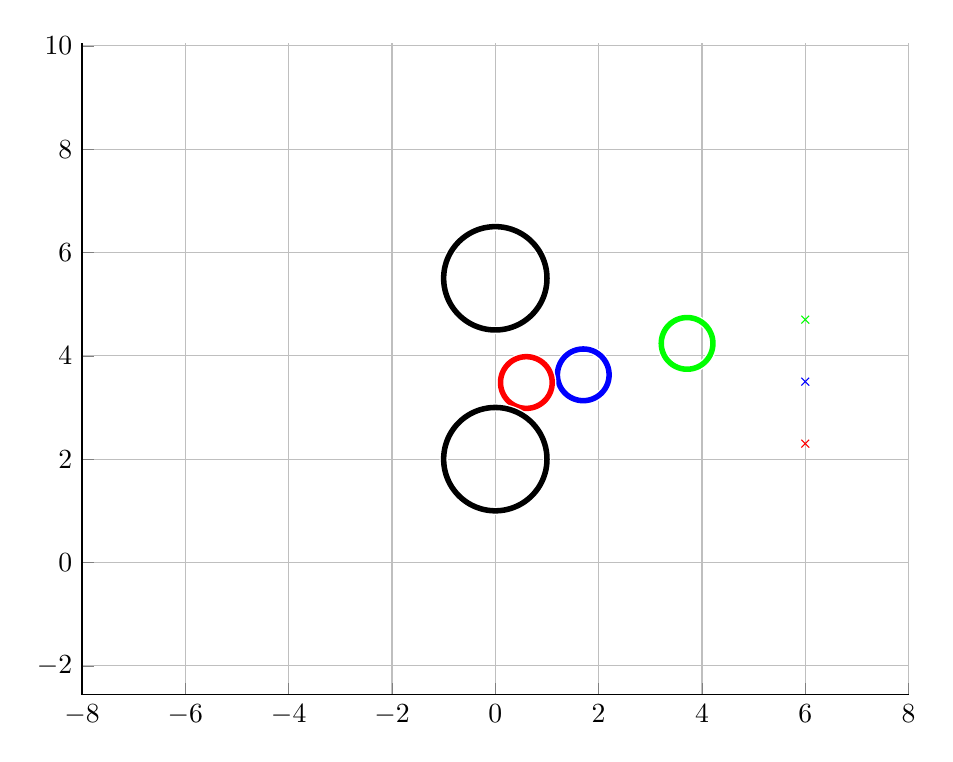
\begin{tikzpicture}

\begin{axis}[%
width=4.133in,
height=3.26in,
at={(0.693in,0.44in)},
scale only axis,
unbounded coords=jump,
xmin=-8,
xmax=8,
xmajorgrids,
ymin=-2.55967741935484,
ymax=10.0596774193548,
ymajorgrids,
axis background/.style={fill=white},
axis x line*=bottom,
axis y line*=left
]
\addplot [color=blue,only marks,mark=x,mark options={solid},forget plot]
  table[row sep=crcr]{%
6	3.5\\
};
\addplot [color=red,only marks,mark=x,mark options={solid},forget plot]
  table[row sep=crcr]{%
6	2.3\\
};
\addplot [color=green,only marks,mark=x,mark options={solid},forget plot]
  table[row sep=crcr]{%
6	4.7\\
};
\addplot [color=white,solid,line width=3.0pt,forget plot]
  table[row sep=crcr]{%
2.20207432723913	3.63177924957654\\
2.20176974074868	3.64922899792779\\
2.20085635236905	3.6666574864486\\
2.19933527492327	3.68404348121036\\
2.19720836160992	3.70136580005657\\
2.19447820374524	3.71860333841\\
2.19114812760604	3.73573509498542\\
2.18722219037713	3.75274019737637\\
2.18270517520829	3.76959792748504\\
2.17760258538671	3.78628774676401\\
2.17192063763209	3.80278932123937\\
2.16566625452253	3.81908254628449\\
2.15884705606044	3.83514757111444\\
2.15147135038872	3.85096482297108\\
2.1435481236686	3.86651503096948\\
2.13508702913135	3.88177924957654\\
2.12609837531735	3.89673888169314\\
2.11659311351666	3.91137570131191\\
2.10658282442661	3.92567187572277\\
2.0960797040425	3.93960998723937\\
2.08509654879862	3.95317305441981\\
2.07364673997783	3.96634455275597\\
2.06174422740846	3.97910843480604\\
2.04940351246863	3.99144914974586\\
2.03663963041856	4.00335166231523\\
2.0234681320824	4.01480147113603\\
2.00990506490196	4.0257846263799\\
1.99596695338537	4.03628774676401\\
1.98167077897451	4.04629803585406\\
1.96703395935574	4.05580329765475\\
1.95207432723913	4.06479195146876\\
1.93681010863208	4.073253046006\\
1.92125990063367	4.08117627272612\\
1.90544264877704	4.08855197839784\\
1.88937762394709	4.09537117685993\\
1.87308439890197	4.10162555996949\\
1.85658282442661	4.10730750772411\\
1.83989300514763	4.1124100975457\\
1.82303527503897	4.11692711271454\\
1.80603017264801	4.12085304994344\\
1.7888984160726	4.12418312608264\\
1.77166087771917	4.12691328394732\\
1.75433855887296	4.12904019726067\\
1.7369525641112	4.13056127470645\\
1.71952407559039	4.13147466308609\\
1.70207432723913	4.13177924957654\\
1.68462457888788	4.13147466308609\\
1.66719609036707	4.13056127470645\\
1.64981009560531	4.12904019726067\\
1.6324877767591	4.12691328394732\\
1.61525023840567	4.12418312608264\\
1.59811848183026	4.12085304994344\\
1.5811133794393	4.11692711271454\\
1.56425564933064	4.1124100975457\\
1.54756583005166	4.10730750772411\\
1.5310642555763	4.10162555996949\\
1.51477103053118	4.09537117685993\\
1.49870600570123	4.08855197839784\\
1.4828887538446	4.08117627272612\\
1.46733854584619	4.073253046006\\
1.45207432723913	4.06479195146876\\
1.43711469512253	4.05580329765475\\
1.42247787550376	4.04629803585406\\
1.4081817010929	4.03628774676401\\
1.39424358957631	4.0257846263799\\
1.38068052239587	4.01480147113603\\
1.36750902405971	4.00335166231523\\
1.35474514200964	3.99144914974586\\
1.34240442706981	3.97910843480604\\
1.33050191450044	3.96634455275597\\
1.31905210567965	3.95317305441981\\
1.30806895043577	3.93960998723937\\
1.29756583005166	3.92567187572277\\
1.28755554096161	3.91137570131191\\
1.27805027916092	3.89673888169314\\
1.26906162534692	3.88177924957654\\
1.26060053080967	3.86651503096948\\
1.25267730408955	3.85096482297108\\
1.24530159841783	3.83514757111444\\
1.23848239995574	3.81908254628449\\
1.23222801684618	3.80278932123937\\
1.22654606909156	3.78628774676401\\
1.22144347926998	3.76959792748504\\
1.21692646410114	3.75274019737637\\
1.21300052687223	3.73573509498542\\
1.20967045073303	3.71860333841\\
1.20694029286835	3.70136580005657\\
1.204813379555	3.68404348121036\\
1.20329230210922	3.6666574864486\\
1.20237891372959	3.64922899792779\\
1.20207432723913	3.63177924957654\\
1.20237891372959	3.61432950122529\\
1.20329230210922	3.59690101270448\\
1.204813379555	3.57951501794271\\
1.20694029286835	3.5621926990965\\
1.20967045073303	3.54495516074307\\
1.21300052687223	3.52782340416766\\
1.21692646410114	3.5108183017767\\
1.22144347926998	3.49396057166804\\
1.22654606909156	3.47727075238906\\
1.23222801684618	3.4607691779137\\
1.23848239995574	3.44447595286858\\
1.24530159841783	3.42841092803864\\
1.25267730408955	3.412593676182\\
1.26060053080967	3.39704346818359\\
1.26906162534692	3.38177924957654\\
1.27805027916092	3.36681961745994\\
1.28755554096161	3.35218279784116\\
1.29756583005166	3.3378866234303\\
1.30806895043577	3.32394851191371\\
1.31905210567965	3.31038544473327\\
1.33050191450044	3.29721394639711\\
1.34240442706981	3.28445006434704\\
1.35474514200964	3.27210934940721\\
1.36750902405971	3.26020683683784\\
1.38068052239587	3.24875702801705\\
1.39424358957631	3.23777387277318\\
1.4081817010929	3.22727075238906\\
1.42247787550376	3.21726046329902\\
1.43711469512253	3.20775520149832\\
1.45207432723913	3.19876654768432\\
1.46733854584619	3.19030545314707\\
1.4828887538446	3.18238222642695\\
1.49870600570123	3.17500652075524\\
1.51477103053118	3.16818732229314\\
1.5310642555763	3.16193293918358\\
1.54756583005166	3.15625099142896\\
1.56425564933064	3.15114840160738\\
1.5811133794393	3.14663138643854\\
1.59811848183026	3.14270544920963\\
1.61525023840567	3.13937537307043\\
1.6324877767591	3.13664521520575\\
1.64981009560531	3.1345183018924\\
1.66719609036707	3.13299722444663\\
1.68462457888788	3.13208383606699\\
1.70207432723913	3.13177924957654\\
1.71952407559039	3.13208383606699\\
1.7369525641112	3.13299722444663\\
1.75433855887296	3.1345183018924\\
1.77166087771917	3.13664521520575\\
1.7888984160726	3.13937537307043\\
1.80603017264801	3.14270544920963\\
1.82303527503897	3.14663138643854\\
1.83989300514763	3.15114840160738\\
1.85658282442661	3.15625099142896\\
1.87308439890197	3.16193293918358\\
1.88937762394709	3.16818732229314\\
1.90544264877704	3.17500652075524\\
1.92125990063367	3.18238222642695\\
1.93681010863208	3.19030545314707\\
1.95207432723913	3.19876654768432\\
1.96703395935574	3.20775520149832\\
1.98167077897451	3.21726046329902\\
1.99596695338537	3.22727075238906\\
2.00990506490196	3.23777387277318\\
2.0234681320824	3.24875702801705\\
2.03663963041856	3.26020683683784\\
2.04940351246863	3.27210934940721\\
2.06174422740846	3.28445006434704\\
2.07364673997783	3.29721394639711\\
2.08509654879862	3.31038544473327\\
2.0960797040425	3.32394851191371\\
2.10658282442661	3.3378866234303\\
2.11659311351666	3.35218279784116\\
2.12609837531735	3.36681961745993\\
2.13508702913135	3.38177924957654\\
2.1435481236686	3.39704346818359\\
2.15147135038872	3.412593676182\\
2.15884705606044	3.42841092803864\\
2.16566625452253	3.44447595286858\\
2.17192063763209	3.4607691779137\\
2.17760258538671	3.47727075238906\\
2.18270517520829	3.49396057166804\\
2.18722219037713	3.5108183017767\\
2.19114812760604	3.52782340416766\\
2.19447820374524	3.54495516074307\\
2.19720836160992	3.5621926990965\\
2.19933527492327	3.57951501794271\\
2.20085635236905	3.59690101270448\\
2.20176974074868	3.61432950122529\\
2.20207432723913	3.63177924957654\\
nan	nan\\
};
\addplot [color=blue,solid,line width=2.0pt,forget plot]
  table[row sep=crcr]{%
2.20207432723913	3.63177924957654\\
2.20176974074868	3.64922899792779\\
2.20085635236905	3.6666574864486\\
2.19933527492327	3.68404348121036\\
2.19720836160992	3.70136580005657\\
2.19447820374524	3.71860333841\\
2.19114812760604	3.73573509498542\\
2.18722219037713	3.75274019737637\\
2.18270517520829	3.76959792748504\\
2.17760258538671	3.78628774676401\\
2.17192063763209	3.80278932123937\\
2.16566625452253	3.81908254628449\\
2.15884705606044	3.83514757111444\\
2.15147135038872	3.85096482297108\\
2.1435481236686	3.86651503096948\\
2.13508702913135	3.88177924957654\\
2.12609837531735	3.89673888169314\\
2.11659311351666	3.91137570131191\\
2.10658282442661	3.92567187572277\\
2.0960797040425	3.93960998723937\\
2.08509654879862	3.95317305441981\\
2.07364673997783	3.96634455275597\\
2.06174422740846	3.97910843480604\\
2.04940351246863	3.99144914974586\\
2.03663963041856	4.00335166231523\\
2.0234681320824	4.01480147113603\\
2.00990506490196	4.0257846263799\\
1.99596695338537	4.03628774676401\\
1.98167077897451	4.04629803585406\\
1.96703395935574	4.05580329765475\\
1.95207432723913	4.06479195146876\\
1.93681010863208	4.073253046006\\
1.92125990063367	4.08117627272612\\
1.90544264877704	4.08855197839784\\
1.88937762394709	4.09537117685993\\
1.87308439890197	4.10162555996949\\
1.85658282442661	4.10730750772411\\
1.83989300514763	4.1124100975457\\
1.82303527503897	4.11692711271454\\
1.80603017264801	4.12085304994344\\
1.7888984160726	4.12418312608264\\
1.77166087771917	4.12691328394732\\
1.75433855887296	4.12904019726067\\
1.7369525641112	4.13056127470645\\
1.71952407559039	4.13147466308609\\
1.70207432723913	4.13177924957654\\
1.68462457888788	4.13147466308609\\
1.66719609036707	4.13056127470645\\
1.64981009560531	4.12904019726067\\
1.6324877767591	4.12691328394732\\
1.61525023840567	4.12418312608264\\
1.59811848183026	4.12085304994344\\
1.5811133794393	4.11692711271454\\
1.56425564933064	4.1124100975457\\
1.54756583005166	4.10730750772411\\
1.5310642555763	4.10162555996949\\
1.51477103053118	4.09537117685993\\
1.49870600570123	4.08855197839784\\
1.4828887538446	4.08117627272612\\
1.46733854584619	4.073253046006\\
1.45207432723913	4.06479195146876\\
1.43711469512253	4.05580329765475\\
1.42247787550376	4.04629803585406\\
1.4081817010929	4.03628774676401\\
1.39424358957631	4.0257846263799\\
1.38068052239587	4.01480147113603\\
1.36750902405971	4.00335166231523\\
1.35474514200964	3.99144914974586\\
1.34240442706981	3.97910843480604\\
1.33050191450044	3.96634455275597\\
1.31905210567965	3.95317305441981\\
1.30806895043577	3.93960998723937\\
1.29756583005166	3.92567187572277\\
1.28755554096161	3.91137570131191\\
1.27805027916092	3.89673888169314\\
1.26906162534692	3.88177924957654\\
1.26060053080967	3.86651503096948\\
1.25267730408955	3.85096482297108\\
1.24530159841783	3.83514757111444\\
1.23848239995574	3.81908254628449\\
1.23222801684618	3.80278932123937\\
1.22654606909156	3.78628774676401\\
1.22144347926998	3.76959792748504\\
1.21692646410114	3.75274019737637\\
1.21300052687223	3.73573509498542\\
1.20967045073303	3.71860333841\\
1.20694029286835	3.70136580005657\\
1.204813379555	3.68404348121036\\
1.20329230210922	3.6666574864486\\
1.20237891372959	3.64922899792779\\
1.20207432723913	3.63177924957654\\
1.20237891372959	3.61432950122529\\
1.20329230210922	3.59690101270448\\
1.204813379555	3.57951501794271\\
1.20694029286835	3.5621926990965\\
1.20967045073303	3.54495516074307\\
1.21300052687223	3.52782340416766\\
1.21692646410114	3.5108183017767\\
1.22144347926998	3.49396057166804\\
1.22654606909156	3.47727075238906\\
1.23222801684618	3.4607691779137\\
1.23848239995574	3.44447595286858\\
1.24530159841783	3.42841092803864\\
1.25267730408955	3.412593676182\\
1.26060053080967	3.39704346818359\\
1.26906162534692	3.38177924957654\\
1.27805027916092	3.36681961745994\\
1.28755554096161	3.35218279784116\\
1.29756583005166	3.3378866234303\\
1.30806895043577	3.32394851191371\\
1.31905210567965	3.31038544473327\\
1.33050191450044	3.29721394639711\\
1.34240442706981	3.28445006434704\\
1.35474514200964	3.27210934940721\\
1.36750902405971	3.26020683683784\\
1.38068052239587	3.24875702801705\\
1.39424358957631	3.23777387277318\\
1.4081817010929	3.22727075238906\\
1.42247787550376	3.21726046329902\\
1.43711469512253	3.20775520149832\\
1.45207432723913	3.19876654768432\\
1.46733854584619	3.19030545314707\\
1.4828887538446	3.18238222642695\\
1.49870600570123	3.17500652075524\\
1.51477103053118	3.16818732229314\\
1.5310642555763	3.16193293918358\\
1.54756583005166	3.15625099142896\\
1.56425564933064	3.15114840160738\\
1.5811133794393	3.14663138643854\\
1.59811848183026	3.14270544920963\\
1.61525023840567	3.13937537307043\\
1.6324877767591	3.13664521520575\\
1.64981009560531	3.1345183018924\\
1.66719609036707	3.13299722444663\\
1.68462457888788	3.13208383606699\\
1.70207432723913	3.13177924957654\\
1.71952407559039	3.13208383606699\\
1.7369525641112	3.13299722444663\\
1.75433855887296	3.1345183018924\\
1.77166087771917	3.13664521520575\\
1.7888984160726	3.13937537307043\\
1.80603017264801	3.14270544920963\\
1.82303527503897	3.14663138643854\\
1.83989300514763	3.15114840160738\\
1.85658282442661	3.15625099142896\\
1.87308439890197	3.16193293918358\\
1.88937762394709	3.16818732229314\\
1.90544264877704	3.17500652075524\\
1.92125990063367	3.18238222642695\\
1.93681010863208	3.19030545314707\\
1.95207432723913	3.19876654768432\\
1.96703395935574	3.20775520149832\\
1.98167077897451	3.21726046329902\\
1.99596695338537	3.22727075238906\\
2.00990506490196	3.23777387277318\\
2.0234681320824	3.24875702801705\\
2.03663963041856	3.26020683683784\\
2.04940351246863	3.27210934940721\\
2.06174422740846	3.28445006434704\\
2.07364673997783	3.29721394639711\\
2.08509654879862	3.31038544473327\\
2.0960797040425	3.32394851191371\\
2.10658282442661	3.3378866234303\\
2.11659311351666	3.35218279784116\\
2.12609837531735	3.36681961745993\\
2.13508702913135	3.38177924957654\\
2.1435481236686	3.39704346818359\\
2.15147135038872	3.412593676182\\
2.15884705606044	3.42841092803864\\
2.16566625452253	3.44447595286858\\
2.17192063763209	3.4607691779137\\
2.17760258538671	3.47727075238906\\
2.18270517520829	3.49396057166804\\
2.18722219037713	3.5108183017767\\
2.19114812760604	3.52782340416766\\
2.19447820374524	3.54495516074307\\
2.19720836160992	3.5621926990965\\
2.19933527492327	3.57951501794271\\
2.20085635236905	3.59690101270448\\
2.20176974074868	3.61432950122529\\
2.20207432723913	3.63177924957654\\
nan	nan\\
};
\addplot [color=white,solid,line width=3.0pt,forget plot]
  table[row sep=crcr]{%
1.10067419629149	3.48296679325923\\
1.10036960980104	3.50041654161048\\
1.09945622142141	3.51784503013129\\
1.09793514397563	3.53523102489306\\
1.09580823066228	3.55255334373926\\
1.0930780727976	3.5697908820927\\
1.0897479966584	3.58692263866811\\
1.08582205942949	3.60392774105907\\
1.08130504426065	3.62078547116773\\
1.07620245443907	3.63747529044671\\
1.07052050668445	3.65397686492207\\
1.06426612357489	3.67027008996719\\
1.05744692511279	3.68633511479713\\
1.05007121944108	3.70215236665377\\
1.04214799272096	3.71770257465218\\
1.03368689818371	3.73296679325923\\
1.02469824436971	3.74792642537583\\
1.01519298256901	3.76256324499461\\
1.00518269347897	3.77685941940547\\
0.994679573094855	3.79079753092206\\
0.983696417850983	3.8043605981025\\
0.972246609030191	3.81753209643866\\
0.960344096460819	3.83029597848873\\
0.948003381520993	3.84263669342856\\
0.935239499470923	3.85453920599793\\
0.922068001134764	3.86598901481872\\
0.908504933954323	3.87697217006259\\
0.89456682243773	3.88747529044671\\
0.880270648026867	3.89748557953675\\
0.865633828408096	3.90699084133745\\
0.850674196291494	3.91597949515145\\
0.835409977684439	3.9244405896887\\
0.819859769686033	3.93236381640882\\
0.804042517829394	3.93973952208053\\
0.78797749299945	3.94655872054263\\
0.771684267954328	3.95281310365219\\
0.755182693478968	3.95849505140681\\
0.738492874199993	3.96359764122839\\
0.721635144091328	3.96811465639723\\
0.704630041700374	3.97204059362613\\
0.687498285124959	3.97537066976534\\
0.670260746771527	3.97810082763002\\
0.652938427925321	3.98022774094337\\
0.635552433163557	3.98174881838914\\
0.618123944642744	3.98266220676878\\
0.600674196291494	3.98296679325923\\
0.583224447940244	3.98266220676878\\
0.565795959419431	3.98174881838914\\
0.548409964657667	3.98022774094337\\
0.531087645811461	3.97810082763002\\
0.513850107458029	3.97537066976534\\
0.496718350882614	3.97204059362613\\
0.47971324849166	3.96811465639723\\
0.462855518382994	3.96359764122839\\
0.44616569910402	3.95849505140681\\
0.42966412462866	3.95281310365219\\
0.413370899583538	3.94655872054263\\
0.397305874753594	3.93973952208053\\
0.381488622896955	3.93236381640882\\
0.365938414898549	3.9244405896887\\
0.350674196291494	3.91597949515145\\
0.335714564174891	3.90699084133745\\
0.321077744556121	3.89748557953675\\
0.306781570145257	3.88747529044671\\
0.292843458628665	3.87697217006259\\
0.279280391448224	3.86598901481872\\
0.266108893112065	3.85453920599793\\
0.253345011061995	3.84263669342856\\
0.241004296122168	3.83029597848873\\
0.229101783552797	3.81753209643866\\
0.217651974732005	3.8043605981025\\
0.206668819488133	3.79079753092206\\
0.19616569910402	3.77685941940547\\
0.186155410013973	3.76256324499461\\
0.176650148213281	3.74792642537583\\
0.167661494399275	3.73296679325923\\
0.15920039986203	3.71770257465218\\
0.15127717314191	3.70215236665377\\
0.143901467470194	3.68633511479713\\
0.1370822690081	3.67027008996719\\
0.13082788589854	3.65397686492207\\
0.125145938143917	3.63747529044671\\
0.120043348322335	3.62078547116773\\
0.115526333153496	3.60392774105907\\
0.111600395924591	3.58692263866811\\
0.10827031978539	3.5697908820927\\
0.105540161920709	3.55255334373926\\
0.103413248607357	3.53523102489306\\
0.101892171161582	3.51784503013129\\
0.100978782781946	3.50041654161048\\
0.100674196291494	3.48296679325923\\
0.100978782781946	3.46551704490798\\
0.101892171161582	3.44808855638717\\
0.103413248607357	3.43070256162541\\
0.105540161920709	3.4133802427792\\
0.10827031978539	3.39614270442577\\
0.111600395924591	3.37901094785035\\
0.115526333153496	3.3620058454594\\
0.120043348322334	3.34514811535073\\
0.125145938143917	3.32845829607176\\
0.13082788589854	3.3119567215964\\
0.1370822690081	3.29566349655128\\
0.143901467470193	3.27959847172133\\
0.15127717314191	3.26378121986469\\
0.15920039986203	3.24823101186629\\
0.167661494399275	3.23296679325923\\
0.176650148213281	3.21800716114263\\
0.186155410013973	3.20337034152386\\
0.19616569910402	3.189074167113\\
0.206668819488133	3.1751360555964\\
0.217651974732005	3.16157298841596\\
0.229101783552797	3.1484014900798\\
0.241004296122168	3.13563760802973\\
0.253345011061995	3.12329689308991\\
0.266108893112065	3.11139438052053\\
0.279280391448224	3.09994457169974\\
0.292843458628665	3.08896141645587\\
0.306781570145257	3.07845829607176\\
0.32107774455612	3.06844800698171\\
0.335714564174891	3.05894274518102\\
0.350674196291494	3.04995409136701\\
0.365938414898549	3.04149299682977\\
0.381488622896955	3.03356977010965\\
0.397305874753594	3.02619406443793\\
0.413370899583538	3.01937486597584\\
0.429664124628659	3.01312048286628\\
0.44616569910402	3.00743853511166\\
0.462855518382994	3.00233594529007\\
0.47971324849166	2.99781893012123\\
0.496718350882614	2.99389299289233\\
0.513850107458029	2.99056291675313\\
0.531087645811461	2.98783275888845\\
0.548409964657667	2.9857058455751\\
0.565795959419431	2.98418476812932\\
0.583224447940243	2.98327137974968\\
0.600674196291494	2.98296679325923\\
0.618123944642745	2.98327137974968\\
0.635552433163556	2.98418476812932\\
0.65293842792532	2.9857058455751\\
0.670260746771527	2.98783275888845\\
0.687498285124959	2.99056291675313\\
0.704630041700373	2.99389299289233\\
0.721635144091328	2.99781893012123\\
0.738492874199994	3.00233594529007\\
0.755182693478967	3.00743853511166\\
0.771684267954328	3.01312048286628\\
0.78797749299945	3.01937486597584\\
0.804042517829394	3.02619406443793\\
0.819859769686033	3.03356977010965\\
0.835409977684439	3.04149299682977\\
0.850674196291494	3.04995409136701\\
0.865633828408096	3.05894274518102\\
0.880270648026867	3.06844800698171\\
0.89456682243773	3.07845829607176\\
0.908504933954323	3.08896141645587\\
0.922068001134764	3.09994457169974\\
0.935239499470923	3.11139438052053\\
0.948003381520992	3.12329689308991\\
0.960344096460819	3.13563760802973\\
0.972246609030191	3.1484014900798\\
0.983696417850983	3.16157298841596\\
0.994679573094855	3.1751360555964\\
1.00518269347897	3.189074167113\\
1.01519298256901	3.20337034152386\\
1.02469824436971	3.21800716114263\\
1.03368689818371	3.23296679325923\\
1.04214799272096	3.24823101186629\\
1.05007121944108	3.26378121986469\\
1.05744692511279	3.27959847172133\\
1.06426612357489	3.29566349655128\\
1.07052050668445	3.3119567215964\\
1.07620245443907	3.32845829607176\\
1.08130504426065	3.34514811535073\\
1.08582205942949	3.3620058454594\\
1.0897479966584	3.37901094785035\\
1.0930780727976	3.39614270442577\\
1.09580823066228	3.4133802427792\\
1.09793514397563	3.4307025616254\\
1.09945622142141	3.44808855638717\\
1.10036960980104	3.46551704490798\\
1.10067419629149	3.48296679325923\\
nan	nan\\
};
\addplot [color=red,solid,line width=2.0pt,forget plot]
  table[row sep=crcr]{%
1.10067419629149	3.48296679325923\\
1.10036960980104	3.50041654161048\\
1.09945622142141	3.51784503013129\\
1.09793514397563	3.53523102489306\\
1.09580823066228	3.55255334373926\\
1.0930780727976	3.5697908820927\\
1.0897479966584	3.58692263866811\\
1.08582205942949	3.60392774105907\\
1.08130504426065	3.62078547116773\\
1.07620245443907	3.63747529044671\\
1.07052050668445	3.65397686492207\\
1.06426612357489	3.67027008996719\\
1.05744692511279	3.68633511479713\\
1.05007121944108	3.70215236665377\\
1.04214799272096	3.71770257465218\\
1.03368689818371	3.73296679325923\\
1.02469824436971	3.74792642537583\\
1.01519298256901	3.76256324499461\\
1.00518269347897	3.77685941940547\\
0.994679573094855	3.79079753092206\\
0.983696417850983	3.8043605981025\\
0.972246609030191	3.81753209643866\\
0.960344096460819	3.83029597848873\\
0.948003381520993	3.84263669342856\\
0.935239499470923	3.85453920599793\\
0.922068001134764	3.86598901481872\\
0.908504933954323	3.87697217006259\\
0.89456682243773	3.88747529044671\\
0.880270648026867	3.89748557953675\\
0.865633828408096	3.90699084133745\\
0.850674196291494	3.91597949515145\\
0.835409977684439	3.9244405896887\\
0.819859769686033	3.93236381640882\\
0.804042517829394	3.93973952208053\\
0.78797749299945	3.94655872054263\\
0.771684267954328	3.95281310365219\\
0.755182693478968	3.95849505140681\\
0.738492874199993	3.96359764122839\\
0.721635144091328	3.96811465639723\\
0.704630041700374	3.97204059362613\\
0.687498285124959	3.97537066976534\\
0.670260746771527	3.97810082763002\\
0.652938427925321	3.98022774094337\\
0.635552433163557	3.98174881838914\\
0.618123944642744	3.98266220676878\\
0.600674196291494	3.98296679325923\\
0.583224447940244	3.98266220676878\\
0.565795959419431	3.98174881838914\\
0.548409964657667	3.98022774094337\\
0.531087645811461	3.97810082763002\\
0.513850107458029	3.97537066976534\\
0.496718350882614	3.97204059362613\\
0.47971324849166	3.96811465639723\\
0.462855518382994	3.96359764122839\\
0.44616569910402	3.95849505140681\\
0.42966412462866	3.95281310365219\\
0.413370899583538	3.94655872054263\\
0.397305874753594	3.93973952208053\\
0.381488622896955	3.93236381640882\\
0.365938414898549	3.9244405896887\\
0.350674196291494	3.91597949515145\\
0.335714564174891	3.90699084133745\\
0.321077744556121	3.89748557953675\\
0.306781570145257	3.88747529044671\\
0.292843458628665	3.87697217006259\\
0.279280391448224	3.86598901481872\\
0.266108893112065	3.85453920599793\\
0.253345011061995	3.84263669342856\\
0.241004296122168	3.83029597848873\\
0.229101783552797	3.81753209643866\\
0.217651974732005	3.8043605981025\\
0.206668819488133	3.79079753092206\\
0.19616569910402	3.77685941940547\\
0.186155410013973	3.76256324499461\\
0.176650148213281	3.74792642537583\\
0.167661494399275	3.73296679325923\\
0.15920039986203	3.71770257465218\\
0.15127717314191	3.70215236665377\\
0.143901467470194	3.68633511479713\\
0.1370822690081	3.67027008996719\\
0.13082788589854	3.65397686492207\\
0.125145938143917	3.63747529044671\\
0.120043348322335	3.62078547116773\\
0.115526333153496	3.60392774105907\\
0.111600395924591	3.58692263866811\\
0.10827031978539	3.5697908820927\\
0.105540161920709	3.55255334373926\\
0.103413248607357	3.53523102489306\\
0.101892171161582	3.51784503013129\\
0.100978782781946	3.50041654161048\\
0.100674196291494	3.48296679325923\\
0.100978782781946	3.46551704490798\\
0.101892171161582	3.44808855638717\\
0.103413248607357	3.43070256162541\\
0.105540161920709	3.4133802427792\\
0.10827031978539	3.39614270442577\\
0.111600395924591	3.37901094785035\\
0.115526333153496	3.3620058454594\\
0.120043348322334	3.34514811535073\\
0.125145938143917	3.32845829607176\\
0.13082788589854	3.3119567215964\\
0.1370822690081	3.29566349655128\\
0.143901467470193	3.27959847172133\\
0.15127717314191	3.26378121986469\\
0.15920039986203	3.24823101186629\\
0.167661494399275	3.23296679325923\\
0.176650148213281	3.21800716114263\\
0.186155410013973	3.20337034152386\\
0.19616569910402	3.189074167113\\
0.206668819488133	3.1751360555964\\
0.217651974732005	3.16157298841596\\
0.229101783552797	3.1484014900798\\
0.241004296122168	3.13563760802973\\
0.253345011061995	3.12329689308991\\
0.266108893112065	3.11139438052053\\
0.279280391448224	3.09994457169974\\
0.292843458628665	3.08896141645587\\
0.306781570145257	3.07845829607176\\
0.32107774455612	3.06844800698171\\
0.335714564174891	3.05894274518102\\
0.350674196291494	3.04995409136701\\
0.365938414898549	3.04149299682977\\
0.381488622896955	3.03356977010965\\
0.397305874753594	3.02619406443793\\
0.413370899583538	3.01937486597584\\
0.429664124628659	3.01312048286628\\
0.44616569910402	3.00743853511166\\
0.462855518382994	3.00233594529007\\
0.47971324849166	2.99781893012123\\
0.496718350882614	2.99389299289233\\
0.513850107458029	2.99056291675313\\
0.531087645811461	2.98783275888845\\
0.548409964657667	2.9857058455751\\
0.565795959419431	2.98418476812932\\
0.583224447940243	2.98327137974968\\
0.600674196291494	2.98296679325923\\
0.618123944642745	2.98327137974968\\
0.635552433163556	2.98418476812932\\
0.65293842792532	2.9857058455751\\
0.670260746771527	2.98783275888845\\
0.687498285124959	2.99056291675313\\
0.704630041700373	2.99389299289233\\
0.721635144091328	2.99781893012123\\
0.738492874199994	3.00233594529007\\
0.755182693478967	3.00743853511166\\
0.771684267954328	3.01312048286628\\
0.78797749299945	3.01937486597584\\
0.804042517829394	3.02619406443793\\
0.819859769686033	3.03356977010965\\
0.835409977684439	3.04149299682977\\
0.850674196291494	3.04995409136701\\
0.865633828408096	3.05894274518102\\
0.880270648026867	3.06844800698171\\
0.89456682243773	3.07845829607176\\
0.908504933954323	3.08896141645587\\
0.922068001134764	3.09994457169974\\
0.935239499470923	3.11139438052053\\
0.948003381520992	3.12329689308991\\
0.960344096460819	3.13563760802973\\
0.972246609030191	3.1484014900798\\
0.983696417850983	3.16157298841596\\
0.994679573094855	3.1751360555964\\
1.00518269347897	3.189074167113\\
1.01519298256901	3.20337034152386\\
1.02469824436971	3.21800716114263\\
1.03368689818371	3.23296679325923\\
1.04214799272096	3.24823101186629\\
1.05007121944108	3.26378121986469\\
1.05744692511279	3.27959847172133\\
1.06426612357489	3.29566349655128\\
1.07052050668445	3.3119567215964\\
1.07620245443907	3.32845829607176\\
1.08130504426065	3.34514811535073\\
1.08582205942949	3.3620058454594\\
1.0897479966584	3.37901094785035\\
1.0930780727976	3.39614270442577\\
1.09580823066228	3.4133802427792\\
1.09793514397563	3.4307025616254\\
1.09945622142141	3.44808855638717\\
1.10036960980104	3.46551704490798\\
1.10067419629149	3.48296679325923\\
nan	nan\\
};
\addplot [color=white,solid,line width=3.0pt,forget plot]
  table[row sep=crcr]{%
4.21193617982375	4.24042966922375\\
4.2116315933333	4.257879417575\\
4.21071820495366	4.27530790609582\\
4.20919712750789	4.29269390085758\\
4.20707021419454	4.31001621970379\\
4.20434005632986	4.32725375805722\\
4.20100998019065	4.34438551463263\\
4.19708404296175	4.36139061702359\\
4.19256702779291	4.37824834713225\\
4.18746443797133	4.39493816641123\\
4.18178249021671	4.41143974088659\\
4.17552810710715	4.42773296593171\\
4.16870890864505	4.44379799076165\\
4.16133320297334	4.45961524261829\\
4.15340997625322	4.4751654506167\\
4.14494888171597	4.49042966922375\\
4.13596022790197	4.50538930134036\\
4.12645496610127	4.52002612095913\\
4.11644467701123	4.53432229536999\\
4.10594155662711	4.54826040688658\\
4.09495840138324	4.56182347406702\\
4.08350859256245	4.57499497240318\\
4.07160607999308	4.58775885445325\\
4.05926536505325	4.60009956939308\\
4.04650148300318	4.61200208196245\\
4.03332998466702	4.62345189078324\\
4.01976691748658	4.63443504602711\\
4.00582880596999	4.64493816641123\\
3.99153263155913	4.65494845550127\\
3.97689581194035	4.66445371730197\\
3.96193617982375	4.67344237111597\\
3.9466719612167	4.68190346565322\\
3.93112175321829	4.68982669237334\\
3.91530450136165	4.69720239804505\\
3.89923947653171	4.70402159650715\\
3.88294625148659	4.71027597961671\\
3.86644467701123	4.71595792737133\\
3.84975485773225	4.72106051719291\\
3.83289712762359	4.72557753236175\\
3.81589202523263	4.72950346959066\\
3.79876026865722	4.73283354572986\\
3.78152273030379	4.73556370359454\\
3.76420041145758	4.73769061690789\\
3.74681441669582	4.73921169435367\\
3.729385928175	4.7401250827333\\
3.71193617982375	4.74042966922375\\
3.6944864314725	4.7401250827333\\
3.67705794295169	4.73921169435367\\
3.65967194818993	4.73769061690789\\
3.64234962934372	4.73556370359454\\
3.62511209099029	4.73283354572986\\
3.60798033441487	4.72950346959066\\
3.59097523202392	4.72557753236175\\
3.57411750191525	4.72106051719291\\
3.55742768263628	4.71595792737133\\
3.54092610816092	4.71027597961671\\
3.5246328831158	4.70402159650715\\
3.50856785828585	4.69720239804505\\
3.49275060642921	4.68982669237334\\
3.47720039843081	4.68190346565322\\
3.46193617982375	4.67344237111597\\
3.44697654770715	4.66445371730197\\
3.43233972808838	4.65494845550127\\
3.41804355367752	4.64493816641123\\
3.40410544216092	4.63443504602711\\
3.39054237498048	4.62345189078324\\
3.37737087664432	4.61200208196245\\
3.36460699459425	4.60009956939308\\
3.35226627965443	4.58775885445325\\
3.34036376708506	4.57499497240318\\
3.32891395826426	4.56182347406702\\
3.31793080302039	4.54826040688658\\
3.30742768263628	4.53432229536999\\
3.29741739354623	4.52002612095913\\
3.28791213174554	4.50538930134036\\
3.27892347793153	4.49042966922375\\
3.27046238339429	4.4751654506167\\
3.26253915667417	4.45961524261829\\
3.25516345100245	4.44379799076165\\
3.24834425254036	4.42773296593171\\
3.2420898694308	4.41143974088659\\
3.23640792167618	4.39493816641123\\
3.23130533185459	4.37824834713225\\
3.22678831668575	4.36139061702359\\
3.22286237945685	4.34438551463263\\
3.21953230331765	4.32725375805722\\
3.21680214545297	4.31001621970379\\
3.21467523213962	4.29269390085758\\
3.21315415469384	4.27530790609582\\
3.2122407663142	4.257879417575\\
3.21193617982375	4.24042966922375\\
3.2122407663142	4.2229799208725\\
3.21315415469384	4.20555143235169\\
3.21467523213962	4.18816543758993\\
3.21680214545297	4.17084311874372\\
3.21953230331765	4.15360558039029\\
3.22286237945685	4.13647382381487\\
3.22678831668575	4.11946872142392\\
3.23130533185459	4.10261099131525\\
3.23640792167618	4.08592117203628\\
3.2420898694308	4.06941959756092\\
3.24834425254036	4.0531263725158\\
3.25516345100245	4.03706134768585\\
3.26253915667417	4.02124409582922\\
3.27046238339429	4.00569388783081\\
3.27892347793153	3.99042966922375\\
3.28791213174554	3.97547003710715\\
3.29741739354623	3.96083321748838\\
3.30742768263628	3.94653704307752\\
3.31793080302039	3.93259893156092\\
3.32891395826426	3.91903586438048\\
3.34036376708506	3.90586436604432\\
3.35226627965443	3.89310048399425\\
3.36460699459425	3.88075976905443\\
3.37737087664432	3.86885725648506\\
3.39054237498048	3.85740744766426\\
3.40410544216092	3.84642429242039\\
3.41804355367752	3.83592117203628\\
3.43233972808838	3.82591088294623\\
3.44697654770715	3.81640562114554\\
3.46193617982375	3.80741696733153\\
3.47720039843081	3.79895587279429\\
3.49275060642921	3.79103264607417\\
3.50856785828585	3.78365694040245\\
3.5246328831158	3.77683774194036\\
3.54092610816092	3.7705833588308\\
3.55742768263628	3.76490141107618\\
3.57411750191525	3.75979882125459\\
3.59097523202392	3.75528180608576\\
3.60798033441487	3.75135586885685\\
3.62511209099029	3.74802579271765\\
3.64234962934372	3.74529563485297\\
3.65967194818993	3.74316872153962\\
3.67705794295169	3.74164764409384\\
3.6944864314725	3.74073425571421\\
3.71193617982375	3.74042966922375\\
3.729385928175	3.74073425571421\\
3.74681441669582	3.74164764409384\\
3.76420041145758	3.74316872153962\\
3.78152273030379	3.74529563485297\\
3.79876026865722	3.74802579271765\\
3.81589202523263	3.75135586885685\\
3.83289712762359	3.75528180608576\\
3.84975485773225	3.75979882125459\\
3.86644467701123	3.76490141107618\\
3.88294625148659	3.7705833588308\\
3.89923947653171	3.77683774194036\\
3.91530450136165	3.78365694040245\\
3.93112175321829	3.79103264607417\\
3.9466719612167	3.79895587279429\\
3.96193617982375	3.80741696733153\\
3.97689581194035	3.81640562114554\\
3.99153263155913	3.82591088294623\\
4.00582880596999	3.83592117203628\\
4.01976691748658	3.84642429242039\\
4.03332998466702	3.85740744766426\\
4.04650148300318	3.86885725648506\\
4.05926536505325	3.88075976905443\\
4.07160607999308	3.89310048399425\\
4.08350859256245	3.90586436604432\\
4.09495840138324	3.91903586438048\\
4.10594155662711	3.93259893156092\\
4.11644467701123	3.94653704307752\\
4.12645496610127	3.96083321748838\\
4.13596022790196	3.97547003710715\\
4.14494888171597	3.99042966922375\\
4.15340997625322	4.00569388783081\\
4.16133320297334	4.02124409582922\\
4.16870890864505	4.03706134768585\\
4.17552810710715	4.0531263725158\\
4.18178249021671	4.06941959756092\\
4.18746443797133	4.08592117203628\\
4.19256702779291	4.10261099131525\\
4.19708404296175	4.11946872142392\\
4.20100998019065	4.13647382381487\\
4.20434005632986	4.15360558039029\\
4.20707021419454	4.17084311874372\\
4.20919712750789	4.18816543758993\\
4.21071820495366	4.20555143235169\\
4.2116315933333	4.2229799208725\\
4.21193617982375	4.24042966922375\\
nan	nan\\
};
\addplot [color=green,solid,line width=2.0pt,forget plot]
  table[row sep=crcr]{%
4.21193617982375	4.24042966922375\\
4.2116315933333	4.257879417575\\
4.21071820495366	4.27530790609582\\
4.20919712750789	4.29269390085758\\
4.20707021419454	4.31001621970379\\
4.20434005632986	4.32725375805722\\
4.20100998019065	4.34438551463263\\
4.19708404296175	4.36139061702359\\
4.19256702779291	4.37824834713225\\
4.18746443797133	4.39493816641123\\
4.18178249021671	4.41143974088659\\
4.17552810710715	4.42773296593171\\
4.16870890864505	4.44379799076165\\
4.16133320297334	4.45961524261829\\
4.15340997625322	4.4751654506167\\
4.14494888171597	4.49042966922375\\
4.13596022790197	4.50538930134036\\
4.12645496610127	4.52002612095913\\
4.11644467701123	4.53432229536999\\
4.10594155662711	4.54826040688658\\
4.09495840138324	4.56182347406702\\
4.08350859256245	4.57499497240318\\
4.07160607999308	4.58775885445325\\
4.05926536505325	4.60009956939308\\
4.04650148300318	4.61200208196245\\
4.03332998466702	4.62345189078324\\
4.01976691748658	4.63443504602711\\
4.00582880596999	4.64493816641123\\
3.99153263155913	4.65494845550127\\
3.97689581194035	4.66445371730197\\
3.96193617982375	4.67344237111597\\
3.9466719612167	4.68190346565322\\
3.93112175321829	4.68982669237334\\
3.91530450136165	4.69720239804505\\
3.89923947653171	4.70402159650715\\
3.88294625148659	4.71027597961671\\
3.86644467701123	4.71595792737133\\
3.84975485773225	4.72106051719291\\
3.83289712762359	4.72557753236175\\
3.81589202523263	4.72950346959066\\
3.79876026865722	4.73283354572986\\
3.78152273030379	4.73556370359454\\
3.76420041145758	4.73769061690789\\
3.74681441669582	4.73921169435367\\
3.729385928175	4.7401250827333\\
3.71193617982375	4.74042966922375\\
3.6944864314725	4.7401250827333\\
3.67705794295169	4.73921169435367\\
3.65967194818993	4.73769061690789\\
3.64234962934372	4.73556370359454\\
3.62511209099029	4.73283354572986\\
3.60798033441487	4.72950346959066\\
3.59097523202392	4.72557753236175\\
3.57411750191525	4.72106051719291\\
3.55742768263628	4.71595792737133\\
3.54092610816092	4.71027597961671\\
3.5246328831158	4.70402159650715\\
3.50856785828585	4.69720239804505\\
3.49275060642921	4.68982669237334\\
3.47720039843081	4.68190346565322\\
3.46193617982375	4.67344237111597\\
3.44697654770715	4.66445371730197\\
3.43233972808838	4.65494845550127\\
3.41804355367752	4.64493816641123\\
3.40410544216092	4.63443504602711\\
3.39054237498048	4.62345189078324\\
3.37737087664432	4.61200208196245\\
3.36460699459425	4.60009956939308\\
3.35226627965443	4.58775885445325\\
3.34036376708506	4.57499497240318\\
3.32891395826426	4.56182347406702\\
3.31793080302039	4.54826040688658\\
3.30742768263628	4.53432229536999\\
3.29741739354623	4.52002612095913\\
3.28791213174554	4.50538930134036\\
3.27892347793153	4.49042966922375\\
3.27046238339429	4.4751654506167\\
3.26253915667417	4.45961524261829\\
3.25516345100245	4.44379799076165\\
3.24834425254036	4.42773296593171\\
3.2420898694308	4.41143974088659\\
3.23640792167618	4.39493816641123\\
3.23130533185459	4.37824834713225\\
3.22678831668575	4.36139061702359\\
3.22286237945685	4.34438551463263\\
3.21953230331765	4.32725375805722\\
3.21680214545297	4.31001621970379\\
3.21467523213962	4.29269390085758\\
3.21315415469384	4.27530790609582\\
3.2122407663142	4.257879417575\\
3.21193617982375	4.24042966922375\\
3.2122407663142	4.2229799208725\\
3.21315415469384	4.20555143235169\\
3.21467523213962	4.18816543758993\\
3.21680214545297	4.17084311874372\\
3.21953230331765	4.15360558039029\\
3.22286237945685	4.13647382381487\\
3.22678831668575	4.11946872142392\\
3.23130533185459	4.10261099131525\\
3.23640792167618	4.08592117203628\\
3.2420898694308	4.06941959756092\\
3.24834425254036	4.0531263725158\\
3.25516345100245	4.03706134768585\\
3.26253915667417	4.02124409582922\\
3.27046238339429	4.00569388783081\\
3.27892347793153	3.99042966922375\\
3.28791213174554	3.97547003710715\\
3.29741739354623	3.96083321748838\\
3.30742768263628	3.94653704307752\\
3.31793080302039	3.93259893156092\\
3.32891395826426	3.91903586438048\\
3.34036376708506	3.90586436604432\\
3.35226627965443	3.89310048399425\\
3.36460699459425	3.88075976905443\\
3.37737087664432	3.86885725648506\\
3.39054237498048	3.85740744766426\\
3.40410544216092	3.84642429242039\\
3.41804355367752	3.83592117203628\\
3.43233972808838	3.82591088294623\\
3.44697654770715	3.81640562114554\\
3.46193617982375	3.80741696733153\\
3.47720039843081	3.79895587279429\\
3.49275060642921	3.79103264607417\\
3.50856785828585	3.78365694040245\\
3.5246328831158	3.77683774194036\\
3.54092610816092	3.7705833588308\\
3.55742768263628	3.76490141107618\\
3.57411750191525	3.75979882125459\\
3.59097523202392	3.75528180608576\\
3.60798033441487	3.75135586885685\\
3.62511209099029	3.74802579271765\\
3.64234962934372	3.74529563485297\\
3.65967194818993	3.74316872153962\\
3.67705794295169	3.74164764409384\\
3.6944864314725	3.74073425571421\\
3.71193617982375	3.74042966922375\\
3.729385928175	3.74073425571421\\
3.74681441669582	3.74164764409384\\
3.76420041145758	3.74316872153962\\
3.78152273030379	3.74529563485297\\
3.79876026865722	3.74802579271765\\
3.81589202523263	3.75135586885685\\
3.83289712762359	3.75528180608576\\
3.84975485773225	3.75979882125459\\
3.86644467701123	3.76490141107618\\
3.88294625148659	3.7705833588308\\
3.89923947653171	3.77683774194036\\
3.91530450136165	3.78365694040245\\
3.93112175321829	3.79103264607417\\
3.9466719612167	3.79895587279429\\
3.96193617982375	3.80741696733153\\
3.97689581194035	3.81640562114554\\
3.99153263155913	3.82591088294623\\
4.00582880596999	3.83592117203628\\
4.01976691748658	3.84642429242039\\
4.03332998466702	3.85740744766426\\
4.04650148300318	3.86885725648506\\
4.05926536505325	3.88075976905443\\
4.07160607999308	3.89310048399425\\
4.08350859256245	3.90586436604432\\
4.09495840138324	3.91903586438048\\
4.10594155662711	3.93259893156092\\
4.11644467701123	3.94653704307752\\
4.12645496610127	3.96083321748838\\
4.13596022790196	3.97547003710715\\
4.14494888171597	3.99042966922375\\
4.15340997625322	4.00569388783081\\
4.16133320297334	4.02124409582922\\
4.16870890864505	4.03706134768585\\
4.17552810710715	4.0531263725158\\
4.18178249021671	4.06941959756092\\
4.18746443797133	4.08592117203628\\
4.19256702779291	4.10261099131525\\
4.19708404296175	4.11946872142392\\
4.20100998019065	4.13647382381487\\
4.20434005632986	4.15360558039029\\
4.20707021419454	4.17084311874372\\
4.20919712750789	4.18816543758993\\
4.21071820495366	4.20555143235169\\
4.2116315933333	4.2229799208725\\
4.21193617982375	4.24042966922375\\
nan	nan\\
};
\addplot [color=white,solid,line width=3.0pt,forget plot]
  table[row sep=crcr]{%
1	2\\
0.999390827019096	2.0348994967025\\
0.997564050259824	2.06975647374413\\
0.994521895368273	2.10452846326765\\
0.99026806874157	2.13917310096007\\
0.984807753012208	2.17364817766693\\
0.978147600733806	2.20791169081776\\
0.970295726275996	2.24192189559967\\
0.961261695938319	2.275637355817\\
0.951056516295154	2.30901699437495\\
0.939692620785908	2.34202014332567\\
0.927183854566787	2.37460659341591\\
0.913545457642601	2.4067366430758\\
0.898794046299167	2.43837114678908\\
0.882947592858927	2.46947156278589\\
0.866025403784439	2.5\\
0.848048096156426	2.5299192642332\\
0.829037572555042	2.55919290347075\\
0.809016994374947	2.58778525229247\\
0.788010753606722	2.61566147532566\\
0.766044443118978	2.64278760968654\\
0.743144825477394	2.66913060635886\\
0.719339800338651	2.694658370459\\
0.694658370458997	2.71933980033865\\
0.669130606358858	2.74314482547739\\
0.642787609686539	2.76604444311898\\
0.615661475325658	2.78801075360672\\
0.587785252292473	2.80901699437495\\
0.559192903470747	2.82903757255504\\
0.529919264233205	2.84804809615643\\
0.5	2.86602540378444\\
0.469471562785891	2.88294759285893\\
0.438371146789077	2.89879404629917\\
0.4067366430758	2.9135454576426\\
0.374606593415912	2.92718385456679\\
0.342020143325669	2.93969262078591\\
0.309016994374947	2.95105651629515\\
0.275637355816999	2.96126169593832\\
0.241921895599668	2.970295726276\\
0.207911690817759	2.97814760073381\\
0.17364817766693	2.98480775301221\\
0.139173100960066	2.99026806874157\\
0.104528463267653	2.99452189536827\\
0.0697564737441255	2.99756405025982\\
0.0348994967025011	2.9993908270191\\
6.12323399573677e-17	3\\
-0.0348994967025007	2.9993908270191\\
-0.0697564737441253	2.99756405025982\\
-0.104528463267653	2.99452189536827\\
-0.139173100960065	2.99026806874157\\
-0.17364817766693	2.98480775301221\\
-0.207911690817759	2.97814760073381\\
-0.241921895599668	2.970295726276\\
-0.275637355816999	2.96126169593832\\
-0.309016994374947	2.95105651629515\\
-0.342020143325669	2.93969262078591\\
-0.374606593415912	2.92718385456679\\
-0.4067366430758	2.9135454576426\\
-0.438371146789078	2.89879404629917\\
-0.469471562785891	2.88294759285893\\
-0.5	2.86602540378444\\
-0.529919264233205	2.84804809615643\\
-0.559192903470747	2.82903757255504\\
-0.587785252292473	2.80901699437495\\
-0.615661475325658	2.78801075360672\\
-0.642787609686539	2.76604444311898\\
-0.669130606358858	2.74314482547739\\
-0.694658370458997	2.71933980033865\\
-0.719339800338651	2.694658370459\\
-0.743144825477394	2.66913060635886\\
-0.766044443118978	2.64278760968654\\
-0.788010753606722	2.61566147532566\\
-0.809016994374947	2.58778525229247\\
-0.829037572555042	2.55919290347075\\
-0.848048096156426	2.5299192642332\\
-0.866025403784439	2.5\\
-0.882947592858927	2.46947156278589\\
-0.898794046299167	2.43837114678908\\
-0.913545457642601	2.4067366430758\\
-0.927183854566787	2.37460659341591\\
-0.939692620785908	2.34202014332567\\
-0.951056516295154	2.30901699437495\\
-0.961261695938319	2.275637355817\\
-0.970295726275996	2.24192189559967\\
-0.978147600733806	2.20791169081776\\
-0.984807753012208	2.17364817766693\\
-0.99026806874157	2.13917310096007\\
-0.994521895368273	2.10452846326765\\
-0.997564050259824	2.06975647374413\\
-0.999390827019096	2.0348994967025\\
-1	2\\
-0.999390827019096	1.9651005032975\\
-0.997564050259824	1.93024352625588\\
-0.994521895368273	1.89547153673235\\
-0.99026806874157	1.86082689903993\\
-0.984807753012208	1.82635182233307\\
-0.978147600733806	1.79208830918224\\
-0.970295726275997	1.75807810440033\\
-0.961261695938319	1.724362644183\\
-0.951056516295154	1.69098300562505\\
-0.939692620785908	1.65797985667433\\
-0.927183854566787	1.62539340658409\\
-0.913545457642601	1.5932633569242\\
-0.898794046299167	1.56162885321092\\
-0.882947592858927	1.53052843721411\\
-0.866025403784439	1.5\\
-0.848048096156426	1.4700807357668\\
-0.829037572555042	1.44080709652925\\
-0.809016994374947	1.41221474770753\\
-0.788010753606722	1.38433852467434\\
-0.766044443118978	1.35721239031346\\
-0.743144825477394	1.33086939364114\\
-0.719339800338651	1.305341629541\\
-0.694658370458997	1.28066019966135\\
-0.669130606358858	1.25685517452261\\
-0.642787609686539	1.23395555688102\\
-0.615661475325658	1.21198924639328\\
-0.587785252292473	1.19098300562505\\
-0.559192903470747	1.17096242744496\\
-0.529919264233205	1.15195190384357\\
-0.5	1.13397459621556\\
-0.469471562785891	1.11705240714107\\
-0.438371146789078	1.10120595370083\\
-0.4067366430758	1.0864545423574\\
-0.374606593415912	1.07281614543321\\
-0.342020143325669	1.06030737921409\\
-0.309016994374948	1.04894348370485\\
-0.275637355816999	1.03873830406168\\
-0.241921895599668	1.029704273724\\
-0.20791169081776	1.02185239926619\\
-0.17364817766693	1.01519224698779\\
-0.139173100960065	1.00973193125843\\
-0.104528463267653	1.00547810463173\\
-0.0697564737441256	1.00243594974018\\
-0.0348994967025016	1.0006091729809\\
-1.83697019872103e-16	1\\
0.0348994967025013	1.0006091729809\\
0.0697564737441252	1.00243594974018\\
0.104528463267653	1.00547810463173\\
0.139173100960065	1.00973193125843\\
0.17364817766693	1.01519224698779\\
0.207911690817759	1.02185239926619\\
0.241921895599667	1.029704273724\\
0.275637355816999	1.03873830406168\\
0.309016994374947	1.04894348370485\\
0.342020143325668	1.06030737921409\\
0.374606593415912	1.07281614543321\\
0.406736643075801	1.0864545423574\\
0.438371146789077	1.10120595370083\\
0.46947156278589	1.11705240714107\\
0.5	1.13397459621556\\
0.529919264233205	1.15195190384357\\
0.559192903470746	1.17096242744496\\
0.587785252292473	1.19098300562505\\
0.615661475325659	1.21198924639328\\
0.642787609686539	1.23395555688102\\
0.669130606358858	1.25685517452261\\
0.694658370458997	1.28066019966135\\
0.719339800338651	1.305341629541\\
0.743144825477394	1.33086939364114\\
0.766044443118978	1.35721239031346\\
0.788010753606722	1.38433852467434\\
0.809016994374947	1.41221474770753\\
0.829037572555041	1.44080709652925\\
0.848048096156425	1.47008073576679\\
0.866025403784438	1.5\\
0.882947592858927	1.53052843721411\\
0.898794046299167	1.56162885321092\\
0.913545457642601	1.5932633569242\\
0.927183854566787	1.62539340658409\\
0.939692620785908	1.65797985667433\\
0.951056516295154	1.69098300562505\\
0.961261695938319	1.724362644183\\
0.970295726275996	1.75807810440033\\
0.978147600733806	1.79208830918224\\
0.984807753012208	1.82635182233307\\
0.99026806874157	1.86082689903993\\
0.994521895368273	1.89547153673235\\
0.997564050259824	1.93024352625588\\
0.999390827019096	1.9651005032975\\
1	2\\
nan	nan\\
};
\addplot [color=black,solid,line width=2.0pt,forget plot]
  table[row sep=crcr]{%
1	2\\
0.999390827019096	2.0348994967025\\
0.997564050259824	2.06975647374413\\
0.994521895368273	2.10452846326765\\
0.99026806874157	2.13917310096007\\
0.984807753012208	2.17364817766693\\
0.978147600733806	2.20791169081776\\
0.970295726275996	2.24192189559967\\
0.961261695938319	2.275637355817\\
0.951056516295154	2.30901699437495\\
0.939692620785908	2.34202014332567\\
0.927183854566787	2.37460659341591\\
0.913545457642601	2.4067366430758\\
0.898794046299167	2.43837114678908\\
0.882947592858927	2.46947156278589\\
0.866025403784439	2.5\\
0.848048096156426	2.5299192642332\\
0.829037572555042	2.55919290347075\\
0.809016994374947	2.58778525229247\\
0.788010753606722	2.61566147532566\\
0.766044443118978	2.64278760968654\\
0.743144825477394	2.66913060635886\\
0.719339800338651	2.694658370459\\
0.694658370458997	2.71933980033865\\
0.669130606358858	2.74314482547739\\
0.642787609686539	2.76604444311898\\
0.615661475325658	2.78801075360672\\
0.587785252292473	2.80901699437495\\
0.559192903470747	2.82903757255504\\
0.529919264233205	2.84804809615643\\
0.5	2.86602540378444\\
0.469471562785891	2.88294759285893\\
0.438371146789077	2.89879404629917\\
0.4067366430758	2.9135454576426\\
0.374606593415912	2.92718385456679\\
0.342020143325669	2.93969262078591\\
0.309016994374947	2.95105651629515\\
0.275637355816999	2.96126169593832\\
0.241921895599668	2.970295726276\\
0.207911690817759	2.97814760073381\\
0.17364817766693	2.98480775301221\\
0.139173100960066	2.99026806874157\\
0.104528463267653	2.99452189536827\\
0.0697564737441255	2.99756405025982\\
0.0348994967025011	2.9993908270191\\
6.12323399573677e-17	3\\
-0.0348994967025007	2.9993908270191\\
-0.0697564737441253	2.99756405025982\\
-0.104528463267653	2.99452189536827\\
-0.139173100960065	2.99026806874157\\
-0.17364817766693	2.98480775301221\\
-0.207911690817759	2.97814760073381\\
-0.241921895599668	2.970295726276\\
-0.275637355816999	2.96126169593832\\
-0.309016994374947	2.95105651629515\\
-0.342020143325669	2.93969262078591\\
-0.374606593415912	2.92718385456679\\
-0.4067366430758	2.9135454576426\\
-0.438371146789078	2.89879404629917\\
-0.469471562785891	2.88294759285893\\
-0.5	2.86602540378444\\
-0.529919264233205	2.84804809615643\\
-0.559192903470747	2.82903757255504\\
-0.587785252292473	2.80901699437495\\
-0.615661475325658	2.78801075360672\\
-0.642787609686539	2.76604444311898\\
-0.669130606358858	2.74314482547739\\
-0.694658370458997	2.71933980033865\\
-0.719339800338651	2.694658370459\\
-0.743144825477394	2.66913060635886\\
-0.766044443118978	2.64278760968654\\
-0.788010753606722	2.61566147532566\\
-0.809016994374947	2.58778525229247\\
-0.829037572555042	2.55919290347075\\
-0.848048096156426	2.5299192642332\\
-0.866025403784439	2.5\\
-0.882947592858927	2.46947156278589\\
-0.898794046299167	2.43837114678908\\
-0.913545457642601	2.4067366430758\\
-0.927183854566787	2.37460659341591\\
-0.939692620785908	2.34202014332567\\
-0.951056516295154	2.30901699437495\\
-0.961261695938319	2.275637355817\\
-0.970295726275996	2.24192189559967\\
-0.978147600733806	2.20791169081776\\
-0.984807753012208	2.17364817766693\\
-0.99026806874157	2.13917310096007\\
-0.994521895368273	2.10452846326765\\
-0.997564050259824	2.06975647374413\\
-0.999390827019096	2.0348994967025\\
-1	2\\
-0.999390827019096	1.9651005032975\\
-0.997564050259824	1.93024352625588\\
-0.994521895368273	1.89547153673235\\
-0.99026806874157	1.86082689903993\\
-0.984807753012208	1.82635182233307\\
-0.978147600733806	1.79208830918224\\
-0.970295726275997	1.75807810440033\\
-0.961261695938319	1.724362644183\\
-0.951056516295154	1.69098300562505\\
-0.939692620785908	1.65797985667433\\
-0.927183854566787	1.62539340658409\\
-0.913545457642601	1.5932633569242\\
-0.898794046299167	1.56162885321092\\
-0.882947592858927	1.53052843721411\\
-0.866025403784439	1.5\\
-0.848048096156426	1.4700807357668\\
-0.829037572555042	1.44080709652925\\
-0.809016994374947	1.41221474770753\\
-0.788010753606722	1.38433852467434\\
-0.766044443118978	1.35721239031346\\
-0.743144825477394	1.33086939364114\\
-0.719339800338651	1.305341629541\\
-0.694658370458997	1.28066019966135\\
-0.669130606358858	1.25685517452261\\
-0.642787609686539	1.23395555688102\\
-0.615661475325658	1.21198924639328\\
-0.587785252292473	1.19098300562505\\
-0.559192903470747	1.17096242744496\\
-0.529919264233205	1.15195190384357\\
-0.5	1.13397459621556\\
-0.469471562785891	1.11705240714107\\
-0.438371146789078	1.10120595370083\\
-0.4067366430758	1.0864545423574\\
-0.374606593415912	1.07281614543321\\
-0.342020143325669	1.06030737921409\\
-0.309016994374948	1.04894348370485\\
-0.275637355816999	1.03873830406168\\
-0.241921895599668	1.029704273724\\
-0.20791169081776	1.02185239926619\\
-0.17364817766693	1.01519224698779\\
-0.139173100960065	1.00973193125843\\
-0.104528463267653	1.00547810463173\\
-0.0697564737441256	1.00243594974018\\
-0.0348994967025016	1.0006091729809\\
-1.83697019872103e-16	1\\
0.0348994967025013	1.0006091729809\\
0.0697564737441252	1.00243594974018\\
0.104528463267653	1.00547810463173\\
0.139173100960065	1.00973193125843\\
0.17364817766693	1.01519224698779\\
0.207911690817759	1.02185239926619\\
0.241921895599667	1.029704273724\\
0.275637355816999	1.03873830406168\\
0.309016994374947	1.04894348370485\\
0.342020143325668	1.06030737921409\\
0.374606593415912	1.07281614543321\\
0.406736643075801	1.0864545423574\\
0.438371146789077	1.10120595370083\\
0.46947156278589	1.11705240714107\\
0.5	1.13397459621556\\
0.529919264233205	1.15195190384357\\
0.559192903470746	1.17096242744496\\
0.587785252292473	1.19098300562505\\
0.615661475325659	1.21198924639328\\
0.642787609686539	1.23395555688102\\
0.669130606358858	1.25685517452261\\
0.694658370458997	1.28066019966135\\
0.719339800338651	1.305341629541\\
0.743144825477394	1.33086939364114\\
0.766044443118978	1.35721239031346\\
0.788010753606722	1.38433852467434\\
0.809016994374947	1.41221474770753\\
0.829037572555041	1.44080709652925\\
0.848048096156425	1.47008073576679\\
0.866025403784438	1.5\\
0.882947592858927	1.53052843721411\\
0.898794046299167	1.56162885321092\\
0.913545457642601	1.5932633569242\\
0.927183854566787	1.62539340658409\\
0.939692620785908	1.65797985667433\\
0.951056516295154	1.69098300562505\\
0.961261695938319	1.724362644183\\
0.970295726275996	1.75807810440033\\
0.978147600733806	1.79208830918224\\
0.984807753012208	1.82635182233307\\
0.99026806874157	1.86082689903993\\
0.994521895368273	1.89547153673235\\
0.997564050259824	1.93024352625588\\
0.999390827019096	1.9651005032975\\
1	2\\
nan	nan\\
};
\addplot [color=white,solid,line width=3.0pt,forget plot]
  table[row sep=crcr]{%
1	5.5\\
0.999390827019096	5.5348994967025\\
0.997564050259824	5.56975647374413\\
0.994521895368273	5.60452846326765\\
0.99026806874157	5.63917310096007\\
0.984807753012208	5.67364817766693\\
0.978147600733806	5.70791169081776\\
0.970295726275996	5.74192189559967\\
0.961261695938319	5.775637355817\\
0.951056516295154	5.80901699437495\\
0.939692620785908	5.84202014332567\\
0.927183854566787	5.87460659341591\\
0.913545457642601	5.9067366430758\\
0.898794046299167	5.93837114678908\\
0.882947592858927	5.96947156278589\\
0.866025403784439	6\\
0.848048096156426	6.0299192642332\\
0.829037572555042	6.05919290347075\\
0.809016994374947	6.08778525229247\\
0.788010753606722	6.11566147532566\\
0.766044443118978	6.14278760968654\\
0.743144825477394	6.16913060635886\\
0.719339800338651	6.194658370459\\
0.694658370458997	6.21933980033865\\
0.669130606358858	6.24314482547739\\
0.642787609686539	6.26604444311898\\
0.615661475325658	6.28801075360672\\
0.587785252292473	6.30901699437495\\
0.559192903470747	6.32903757255504\\
0.529919264233205	6.34804809615643\\
0.5	6.36602540378444\\
0.469471562785891	6.38294759285893\\
0.438371146789077	6.39879404629917\\
0.4067366430758	6.4135454576426\\
0.374606593415912	6.42718385456679\\
0.342020143325669	6.43969262078591\\
0.309016994374947	6.45105651629515\\
0.275637355816999	6.46126169593832\\
0.241921895599668	6.470295726276\\
0.207911690817759	6.47814760073381\\
0.17364817766693	6.48480775301221\\
0.139173100960066	6.49026806874157\\
0.104528463267653	6.49452189536827\\
0.0697564737441255	6.49756405025982\\
0.0348994967025011	6.4993908270191\\
6.12323399573677e-17	6.5\\
-0.0348994967025007	6.4993908270191\\
-0.0697564737441253	6.49756405025982\\
-0.104528463267653	6.49452189536827\\
-0.139173100960065	6.49026806874157\\
-0.17364817766693	6.48480775301221\\
-0.207911690817759	6.47814760073381\\
-0.241921895599668	6.470295726276\\
-0.275637355816999	6.46126169593832\\
-0.309016994374947	6.45105651629515\\
-0.342020143325669	6.43969262078591\\
-0.374606593415912	6.42718385456679\\
-0.4067366430758	6.4135454576426\\
-0.438371146789078	6.39879404629917\\
-0.469471562785891	6.38294759285893\\
-0.5	6.36602540378444\\
-0.529919264233205	6.34804809615643\\
-0.559192903470747	6.32903757255504\\
-0.587785252292473	6.30901699437495\\
-0.615661475325658	6.28801075360672\\
-0.642787609686539	6.26604444311898\\
-0.669130606358858	6.24314482547739\\
-0.694658370458997	6.21933980033865\\
-0.719339800338651	6.194658370459\\
-0.743144825477394	6.16913060635886\\
-0.766044443118978	6.14278760968654\\
-0.788010753606722	6.11566147532566\\
-0.809016994374947	6.08778525229247\\
-0.829037572555042	6.05919290347075\\
-0.848048096156426	6.0299192642332\\
-0.866025403784439	6\\
-0.882947592858927	5.96947156278589\\
-0.898794046299167	5.93837114678908\\
-0.913545457642601	5.9067366430758\\
-0.927183854566787	5.87460659341591\\
-0.939692620785908	5.84202014332567\\
-0.951056516295154	5.80901699437495\\
-0.961261695938319	5.775637355817\\
-0.970295726275996	5.74192189559967\\
-0.978147600733806	5.70791169081776\\
-0.984807753012208	5.67364817766693\\
-0.99026806874157	5.63917310096007\\
-0.994521895368273	5.60452846326765\\
-0.997564050259824	5.56975647374413\\
-0.999390827019096	5.5348994967025\\
-1	5.5\\
-0.999390827019096	5.4651005032975\\
-0.997564050259824	5.43024352625588\\
-0.994521895368273	5.39547153673235\\
-0.99026806874157	5.36082689903993\\
-0.984807753012208	5.32635182233307\\
-0.978147600733806	5.29208830918224\\
-0.970295726275997	5.25807810440033\\
-0.961261695938319	5.224362644183\\
-0.951056516295154	5.19098300562505\\
-0.939692620785908	5.15797985667433\\
-0.927183854566787	5.12539340658409\\
-0.913545457642601	5.0932633569242\\
-0.898794046299167	5.06162885321092\\
-0.882947592858927	5.03052843721411\\
-0.866025403784439	5\\
-0.848048096156426	4.9700807357668\\
-0.829037572555042	4.94080709652925\\
-0.809016994374947	4.91221474770753\\
-0.788010753606722	4.88433852467434\\
-0.766044443118978	4.85721239031346\\
-0.743144825477394	4.83086939364114\\
-0.719339800338651	4.805341629541\\
-0.694658370458997	4.78066019966135\\
-0.669130606358858	4.75685517452261\\
-0.642787609686539	4.73395555688102\\
-0.615661475325658	4.71198924639328\\
-0.587785252292473	4.69098300562505\\
-0.559192903470747	4.67096242744496\\
-0.529919264233205	4.65195190384357\\
-0.5	4.63397459621556\\
-0.469471562785891	4.61705240714107\\
-0.438371146789078	4.60120595370083\\
-0.4067366430758	4.5864545423574\\
-0.374606593415912	4.57281614543321\\
-0.342020143325669	4.56030737921409\\
-0.309016994374948	4.54894348370485\\
-0.275637355816999	4.53873830406168\\
-0.241921895599668	4.529704273724\\
-0.20791169081776	4.52185239926619\\
-0.17364817766693	4.51519224698779\\
-0.139173100960065	4.50973193125843\\
-0.104528463267653	4.50547810463173\\
-0.0697564737441256	4.50243594974018\\
-0.0348994967025016	4.5006091729809\\
-1.83697019872103e-16	4.5\\
0.0348994967025013	4.5006091729809\\
0.0697564737441252	4.50243594974018\\
0.104528463267653	4.50547810463173\\
0.139173100960065	4.50973193125843\\
0.17364817766693	4.51519224698779\\
0.207911690817759	4.52185239926619\\
0.241921895599667	4.529704273724\\
0.275637355816999	4.53873830406168\\
0.309016994374947	4.54894348370485\\
0.342020143325668	4.56030737921409\\
0.374606593415912	4.57281614543321\\
0.406736643075801	4.5864545423574\\
0.438371146789077	4.60120595370083\\
0.46947156278589	4.61705240714107\\
0.5	4.63397459621556\\
0.529919264233205	4.65195190384357\\
0.559192903470746	4.67096242744496\\
0.587785252292473	4.69098300562505\\
0.615661475325659	4.71198924639328\\
0.642787609686539	4.73395555688102\\
0.669130606358858	4.75685517452261\\
0.694658370458997	4.78066019966135\\
0.719339800338651	4.805341629541\\
0.743144825477394	4.83086939364114\\
0.766044443118978	4.85721239031346\\
0.788010753606722	4.88433852467434\\
0.809016994374947	4.91221474770753\\
0.829037572555041	4.94080709652925\\
0.848048096156425	4.97008073576679\\
0.866025403784438	5\\
0.882947592858927	5.03052843721411\\
0.898794046299167	5.06162885321092\\
0.913545457642601	5.0932633569242\\
0.927183854566787	5.12539340658409\\
0.939692620785908	5.15797985667433\\
0.951056516295154	5.19098300562505\\
0.961261695938319	5.224362644183\\
0.970295726275996	5.25807810440033\\
0.978147600733806	5.29208830918224\\
0.984807753012208	5.32635182233307\\
0.99026806874157	5.36082689903993\\
0.994521895368273	5.39547153673235\\
0.997564050259824	5.43024352625588\\
0.999390827019096	5.4651005032975\\
1	5.5\\
nan	nan\\
};
\addplot [color=black,solid,line width=2.0pt,forget plot]
  table[row sep=crcr]{%
1	5.5\\
0.999390827019096	5.5348994967025\\
0.997564050259824	5.56975647374413\\
0.994521895368273	5.60452846326765\\
0.99026806874157	5.63917310096007\\
0.984807753012208	5.67364817766693\\
0.978147600733806	5.70791169081776\\
0.970295726275996	5.74192189559967\\
0.961261695938319	5.775637355817\\
0.951056516295154	5.80901699437495\\
0.939692620785908	5.84202014332567\\
0.927183854566787	5.87460659341591\\
0.913545457642601	5.9067366430758\\
0.898794046299167	5.93837114678908\\
0.882947592858927	5.96947156278589\\
0.866025403784439	6\\
0.848048096156426	6.0299192642332\\
0.829037572555042	6.05919290347075\\
0.809016994374947	6.08778525229247\\
0.788010753606722	6.11566147532566\\
0.766044443118978	6.14278760968654\\
0.743144825477394	6.16913060635886\\
0.719339800338651	6.194658370459\\
0.694658370458997	6.21933980033865\\
0.669130606358858	6.24314482547739\\
0.642787609686539	6.26604444311898\\
0.615661475325658	6.28801075360672\\
0.587785252292473	6.30901699437495\\
0.559192903470747	6.32903757255504\\
0.529919264233205	6.34804809615643\\
0.5	6.36602540378444\\
0.469471562785891	6.38294759285893\\
0.438371146789077	6.39879404629917\\
0.4067366430758	6.4135454576426\\
0.374606593415912	6.42718385456679\\
0.342020143325669	6.43969262078591\\
0.309016994374947	6.45105651629515\\
0.275637355816999	6.46126169593832\\
0.241921895599668	6.470295726276\\
0.207911690817759	6.47814760073381\\
0.17364817766693	6.48480775301221\\
0.139173100960066	6.49026806874157\\
0.104528463267653	6.49452189536827\\
0.0697564737441255	6.49756405025982\\
0.0348994967025011	6.4993908270191\\
6.12323399573677e-17	6.5\\
-0.0348994967025007	6.4993908270191\\
-0.0697564737441253	6.49756405025982\\
-0.104528463267653	6.49452189536827\\
-0.139173100960065	6.49026806874157\\
-0.17364817766693	6.48480775301221\\
-0.207911690817759	6.47814760073381\\
-0.241921895599668	6.470295726276\\
-0.275637355816999	6.46126169593832\\
-0.309016994374947	6.45105651629515\\
-0.342020143325669	6.43969262078591\\
-0.374606593415912	6.42718385456679\\
-0.4067366430758	6.4135454576426\\
-0.438371146789078	6.39879404629917\\
-0.469471562785891	6.38294759285893\\
-0.5	6.36602540378444\\
-0.529919264233205	6.34804809615643\\
-0.559192903470747	6.32903757255504\\
-0.587785252292473	6.30901699437495\\
-0.615661475325658	6.28801075360672\\
-0.642787609686539	6.26604444311898\\
-0.669130606358858	6.24314482547739\\
-0.694658370458997	6.21933980033865\\
-0.719339800338651	6.194658370459\\
-0.743144825477394	6.16913060635886\\
-0.766044443118978	6.14278760968654\\
-0.788010753606722	6.11566147532566\\
-0.809016994374947	6.08778525229247\\
-0.829037572555042	6.05919290347075\\
-0.848048096156426	6.0299192642332\\
-0.866025403784439	6\\
-0.882947592858927	5.96947156278589\\
-0.898794046299167	5.93837114678908\\
-0.913545457642601	5.9067366430758\\
-0.927183854566787	5.87460659341591\\
-0.939692620785908	5.84202014332567\\
-0.951056516295154	5.80901699437495\\
-0.961261695938319	5.775637355817\\
-0.970295726275996	5.74192189559967\\
-0.978147600733806	5.70791169081776\\
-0.984807753012208	5.67364817766693\\
-0.99026806874157	5.63917310096007\\
-0.994521895368273	5.60452846326765\\
-0.997564050259824	5.56975647374413\\
-0.999390827019096	5.5348994967025\\
-1	5.5\\
-0.999390827019096	5.4651005032975\\
-0.997564050259824	5.43024352625588\\
-0.994521895368273	5.39547153673235\\
-0.99026806874157	5.36082689903993\\
-0.984807753012208	5.32635182233307\\
-0.978147600733806	5.29208830918224\\
-0.970295726275997	5.25807810440033\\
-0.961261695938319	5.224362644183\\
-0.951056516295154	5.19098300562505\\
-0.939692620785908	5.15797985667433\\
-0.927183854566787	5.12539340658409\\
-0.913545457642601	5.0932633569242\\
-0.898794046299167	5.06162885321092\\
-0.882947592858927	5.03052843721411\\
-0.866025403784439	5\\
-0.848048096156426	4.9700807357668\\
-0.829037572555042	4.94080709652925\\
-0.809016994374947	4.91221474770753\\
-0.788010753606722	4.88433852467434\\
-0.766044443118978	4.85721239031346\\
-0.743144825477394	4.83086939364114\\
-0.719339800338651	4.805341629541\\
-0.694658370458997	4.78066019966135\\
-0.669130606358858	4.75685517452261\\
-0.642787609686539	4.73395555688102\\
-0.615661475325658	4.71198924639328\\
-0.587785252292473	4.69098300562505\\
-0.559192903470747	4.67096242744496\\
-0.529919264233205	4.65195190384357\\
-0.5	4.63397459621556\\
-0.469471562785891	4.61705240714107\\
-0.438371146789078	4.60120595370083\\
-0.4067366430758	4.5864545423574\\
-0.374606593415912	4.57281614543321\\
-0.342020143325669	4.56030737921409\\
-0.309016994374948	4.54894348370485\\
-0.275637355816999	4.53873830406168\\
-0.241921895599668	4.529704273724\\
-0.20791169081776	4.52185239926619\\
-0.17364817766693	4.51519224698779\\
-0.139173100960065	4.50973193125843\\
-0.104528463267653	4.50547810463173\\
-0.0697564737441256	4.50243594974018\\
-0.0348994967025016	4.5006091729809\\
-1.83697019872103e-16	4.5\\
0.0348994967025013	4.5006091729809\\
0.0697564737441252	4.50243594974018\\
0.104528463267653	4.50547810463173\\
0.139173100960065	4.50973193125843\\
0.17364817766693	4.51519224698779\\
0.207911690817759	4.52185239926619\\
0.241921895599667	4.529704273724\\
0.275637355816999	4.53873830406168\\
0.309016994374947	4.54894348370485\\
0.342020143325668	4.56030737921409\\
0.374606593415912	4.57281614543321\\
0.406736643075801	4.5864545423574\\
0.438371146789077	4.60120595370083\\
0.46947156278589	4.61705240714107\\
0.5	4.63397459621556\\
0.529919264233205	4.65195190384357\\
0.559192903470746	4.67096242744496\\
0.587785252292473	4.69098300562505\\
0.615661475325659	4.71198924639328\\
0.642787609686539	4.73395555688102\\
0.669130606358858	4.75685517452261\\
0.694658370458997	4.78066019966135\\
0.719339800338651	4.805341629541\\
0.743144825477394	4.83086939364114\\
0.766044443118978	4.85721239031346\\
0.788010753606722	4.88433852467434\\
0.809016994374947	4.91221474770753\\
0.829037572555041	4.94080709652925\\
0.848048096156425	4.97008073576679\\
0.866025403784438	5\\
0.882947592858927	5.03052843721411\\
0.898794046299167	5.06162885321092\\
0.913545457642601	5.0932633569242\\
0.927183854566787	5.12539340658409\\
0.939692620785908	5.15797985667433\\
0.951056516295154	5.19098300562505\\
0.961261695938319	5.224362644183\\
0.970295726275996	5.25807810440033\\
0.978147600733806	5.29208830918224\\
0.984807753012208	5.32635182233307\\
0.99026806874157	5.36082689903993\\
0.994521895368273	5.39547153673235\\
0.997564050259824	5.43024352625588\\
0.999390827019096	5.4651005032975\\
1	5.5\\
nan	nan\\
};
\end{axis}
\end{tikzpicture}%}
      \caption{}
      \label{}
    \end{figure}
  \end{minipage}
\end{minipage}
}

\noindent\makebox[\linewidth][c]{%
\begin{minipage}{\linewidth}
  \begin{minipage}{0.45\linewidth}
    \begin{figure}[H]
      \scalebox{0.7}{% This file was created by matlab2tikz.
%
%The latest updates can be retrieved from
%  http://www.mathworks.com/matlabcentral/fileexchange/22022-matlab2tikz-matlab2tikz
%where you can also make suggestions and rate matlab2tikz.
%
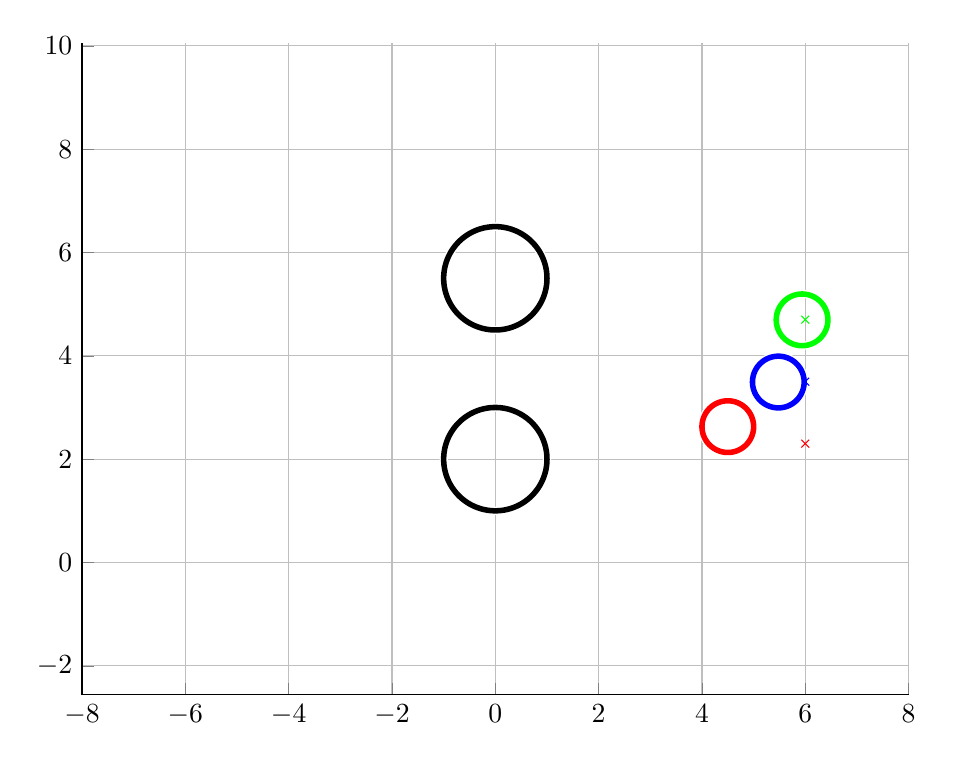
\begin{tikzpicture}

\begin{axis}[%
width=4.133in,
height=3.26in,
at={(0.693in,0.44in)},
scale only axis,
unbounded coords=jump,
xmin=-8,
xmax=8,
xmajorgrids,
ymin=-2.55967741935484,
ymax=10.0596774193548,
ymajorgrids,
axis background/.style={fill=white},
axis x line*=bottom,
axis y line*=left
]
\addplot [color=blue,only marks,mark=x,mark options={solid},forget plot]
  table[row sep=crcr]{%
6	3.5\\
};
\addplot [color=red,only marks,mark=x,mark options={solid},forget plot]
  table[row sep=crcr]{%
6	2.3\\
};
\addplot [color=green,only marks,mark=x,mark options={solid},forget plot]
  table[row sep=crcr]{%
6	4.7\\
};
\addplot [color=white,solid,line width=3.0pt,forget plot]
  table[row sep=crcr]{%
5.97802886291598	3.49251582348264\\
5.97772427642552	3.50996557183389\\
5.97681088804589	3.5273940603547\\
5.97528981060011	3.54478005511646\\
5.97316289728676	3.56210237396267\\
5.97043273942208	3.5793399123161\\
5.96710266328288	3.59647166889152\\
5.96317672605397	3.61347677128247\\
5.95865971088514	3.63033450139114\\
5.95355712106355	3.64702432067011\\
5.94787517330893	3.66352589514547\\
5.94162079019937	3.67981912019059\\
5.93480159173728	3.69588414502054\\
5.92742588606556	3.71170139687717\\
5.91950265934544	3.72725160487558\\
5.9110415648082	3.74251582348264\\
5.90205291099419	3.75747545559924\\
5.8925476491935	3.77211227521801\\
5.88253736010345	3.78640844962887\\
5.87203423971934	3.80034656114546\\
5.86105108447547	3.81390962832591\\
5.84960127565467	3.82708112666207\\
5.8376987630853	3.83984500871213\\
5.82535804814547	3.85218572365196\\
5.8125941660954	3.86408823622133\\
5.79942266775925	3.87553804504212\\
5.78585960057881	3.886521200286\\
5.77192148906221	3.89702432067011\\
5.75762531465135	3.90703460976016\\
5.74298849503258	3.91653987156085\\
5.72802886291598	3.92552852537486\\
5.71276464430892	3.9339896199121\\
5.69721443631051	3.94191284663222\\
5.68139718445388	3.94928855230394\\
5.66533215962393	3.95610775076603\\
5.64903893457881	3.96236213387559\\
5.63253736010345	3.96804408163021\\
5.61584754082448	3.9731466714518\\
5.59898981071581	3.97766368662063\\
5.58198470832486	3.98158962384954\\
5.56485295174944	3.98491969998874\\
5.54761541339601	3.98764985785342\\
5.5302930945498	3.98977677116677\\
5.51290709978804	3.99129784861255\\
5.49547861126723	3.99221123699218\\
5.47802886291598	3.99251582348264\\
5.46057911456473	3.99221123699218\\
5.44315062604391	3.99129784861255\\
5.42576463128215	3.98977677116677\\
5.40844231243594	3.98764985785342\\
5.39120477408251	3.98491969998874\\
5.3740730175071	3.98158962384954\\
5.35706791511614	3.97766368662063\\
5.34021018500748	3.9731466714518\\
5.3235203657285	3.96804408163021\\
5.30701879125314	3.96236213387559\\
5.29072556620802	3.95610775076603\\
5.27466054137808	3.94928855230394\\
5.25884328952144	3.94191284663222\\
5.24329308152303	3.9339896199121\\
5.22802886291598	3.92552852537486\\
5.21306923079937	3.91653987156085\\
5.1984324111806	3.90703460976016\\
5.18413623676974	3.89702432067011\\
5.17019812525315	3.886521200286\\
5.15663505807271	3.87553804504212\\
5.14346355973655	3.86408823622133\\
5.13069967768648	3.85218572365196\\
5.11835896274665	3.83984500871213\\
5.10645645017728	3.82708112666207\\
5.09500664135649	3.81390962832591\\
5.08402348611262	3.80034656114546\\
5.0735203657285	3.78640844962887\\
5.06351007663846	3.77211227521801\\
5.05400481483776	3.75747545559924\\
5.04501616102376	3.74251582348264\\
5.03655506648651	3.72725160487558\\
5.02863183976639	3.71170139687717\\
5.02125613409468	3.69588414502054\\
5.01443693563258	3.67981912019059\\
5.00818255252302	3.66352589514547\\
5.0025006047684	3.64702432067011\\
4.99739801494682	3.63033450139114\\
4.99288099977798	3.61347677128247\\
4.98895506254907	3.59647166889152\\
4.98562498640987	3.5793399123161\\
4.98289482854519	3.56210237396267\\
4.98076791523184	3.54478005511646\\
4.97924683778606	3.5273940603547\\
4.97833344940643	3.50996557183389\\
4.97802886291598	3.49251582348264\\
4.97833344940643	3.47506607513139\\
4.97924683778606	3.45763758661057\\
4.98076791523184	3.44025159184881\\
4.98289482854519	3.4229292730026\\
4.98562498640987	3.40569173464917\\
4.98895506254907	3.38855997807376\\
4.99288099977798	3.3715548756828\\
4.99739801494682	3.35469714557414\\
5.0025006047684	3.33800732629516\\
5.00818255252302	3.3215057518198\\
5.01443693563258	3.30521252677468\\
5.02125613409468	3.28914750194474\\
5.02863183976639	3.2733302500881\\
5.03655506648651	3.25778004208969\\
5.04501616102376	3.24251582348264\\
5.05400481483776	3.22755619136603\\
5.06351007663846	3.21291937174726\\
5.0735203657285	3.1986231973364\\
5.08402348611262	3.18468508581981\\
5.09500664135649	3.17112201863937\\
5.10645645017728	3.15795052030321\\
5.11835896274665	3.14518663825314\\
5.13069967768648	3.13284592331331\\
5.14346355973655	3.12094341074394\\
5.15663505807271	3.10949360192315\\
5.17019812525315	3.09851044667927\\
5.18413623676974	3.08800732629516\\
5.1984324111806	3.07799703720512\\
5.21306923079937	3.06849177540442\\
5.22802886291598	3.05950312159042\\
5.24329308152303	3.05104202705317\\
5.25884328952144	3.04311880033305\\
5.27466054137808	3.03574309466134\\
5.29072556620802	3.02892389619924\\
5.30701879125314	3.02266951308968\\
5.3235203657285	3.01698756533506\\
5.34021018500748	3.01188497551348\\
5.35706791511614	3.00736796034464\\
5.3740730175071	3.00344202311573\\
5.39120477408251	3.00011194697653\\
5.40844231243594	2.99738178911185\\
5.42576463128215	2.9952548757985\\
5.44315062604391	2.99373379835272\\
5.46057911456472	2.99282040997309\\
5.47802886291598	2.99251582348264\\
5.49547861126723	2.99282040997309\\
5.51290709978804	2.99373379835272\\
5.5302930945498	2.9952548757985\\
5.54761541339601	2.99738178911185\\
5.56485295174944	3.00011194697653\\
5.58198470832486	3.00344202311573\\
5.59898981071581	3.00736796034464\\
5.61584754082448	3.01188497551348\\
5.63253736010345	3.01698756533506\\
5.64903893457881	3.02266951308968\\
5.66533215962393	3.02892389619924\\
5.68139718445388	3.03574309466134\\
5.69721443631051	3.04311880033305\\
5.71276464430892	3.05104202705317\\
5.72802886291598	3.05950312159042\\
5.74298849503258	3.06849177540442\\
5.75762531465135	3.07799703720511\\
5.77192148906221	3.08800732629516\\
5.78585960057881	3.09851044667927\\
5.79942266775925	3.10949360192315\\
5.8125941660954	3.12094341074394\\
5.82535804814547	3.13284592331331\\
5.8376987630853	3.14518663825314\\
5.84960127565467	3.15795052030321\\
5.86105108447546	3.17112201863937\\
5.87203423971934	3.18468508581981\\
5.88253736010345	3.1986231973364\\
5.8925476491935	3.21291937174726\\
5.90205291099419	3.22755619136603\\
5.9110415648082	3.24251582348264\\
5.91950265934544	3.25778004208969\\
5.92742588606556	3.2733302500881\\
5.93480159173728	3.28914750194474\\
5.94162079019937	3.30521252677468\\
5.94787517330893	3.3215057518198\\
5.95355712106355	3.33800732629516\\
5.95865971088514	3.35469714557414\\
5.96317672605397	3.3715548756828\\
5.96710266328288	3.38855997807376\\
5.97043273942208	3.40569173464917\\
5.97316289728676	3.4229292730026\\
5.97528981060011	3.44025159184881\\
5.97681088804589	3.45763758661057\\
5.97772427642552	3.47506607513139\\
5.97802886291598	3.49251582348264\\
nan	nan\\
};
\addplot [color=blue,solid,line width=2.0pt,forget plot]
  table[row sep=crcr]{%
5.97802886291598	3.49251582348264\\
5.97772427642552	3.50996557183389\\
5.97681088804589	3.5273940603547\\
5.97528981060011	3.54478005511646\\
5.97316289728676	3.56210237396267\\
5.97043273942208	3.5793399123161\\
5.96710266328288	3.59647166889152\\
5.96317672605397	3.61347677128247\\
5.95865971088514	3.63033450139114\\
5.95355712106355	3.64702432067011\\
5.94787517330893	3.66352589514547\\
5.94162079019937	3.67981912019059\\
5.93480159173728	3.69588414502054\\
5.92742588606556	3.71170139687717\\
5.91950265934544	3.72725160487558\\
5.9110415648082	3.74251582348264\\
5.90205291099419	3.75747545559924\\
5.8925476491935	3.77211227521801\\
5.88253736010345	3.78640844962887\\
5.87203423971934	3.80034656114546\\
5.86105108447547	3.81390962832591\\
5.84960127565467	3.82708112666207\\
5.8376987630853	3.83984500871213\\
5.82535804814547	3.85218572365196\\
5.8125941660954	3.86408823622133\\
5.79942266775925	3.87553804504212\\
5.78585960057881	3.886521200286\\
5.77192148906221	3.89702432067011\\
5.75762531465135	3.90703460976016\\
5.74298849503258	3.91653987156085\\
5.72802886291598	3.92552852537486\\
5.71276464430892	3.9339896199121\\
5.69721443631051	3.94191284663222\\
5.68139718445388	3.94928855230394\\
5.66533215962393	3.95610775076603\\
5.64903893457881	3.96236213387559\\
5.63253736010345	3.96804408163021\\
5.61584754082448	3.9731466714518\\
5.59898981071581	3.97766368662063\\
5.58198470832486	3.98158962384954\\
5.56485295174944	3.98491969998874\\
5.54761541339601	3.98764985785342\\
5.5302930945498	3.98977677116677\\
5.51290709978804	3.99129784861255\\
5.49547861126723	3.99221123699218\\
5.47802886291598	3.99251582348264\\
5.46057911456473	3.99221123699218\\
5.44315062604391	3.99129784861255\\
5.42576463128215	3.98977677116677\\
5.40844231243594	3.98764985785342\\
5.39120477408251	3.98491969998874\\
5.3740730175071	3.98158962384954\\
5.35706791511614	3.97766368662063\\
5.34021018500748	3.9731466714518\\
5.3235203657285	3.96804408163021\\
5.30701879125314	3.96236213387559\\
5.29072556620802	3.95610775076603\\
5.27466054137808	3.94928855230394\\
5.25884328952144	3.94191284663222\\
5.24329308152303	3.9339896199121\\
5.22802886291598	3.92552852537486\\
5.21306923079937	3.91653987156085\\
5.1984324111806	3.90703460976016\\
5.18413623676974	3.89702432067011\\
5.17019812525315	3.886521200286\\
5.15663505807271	3.87553804504212\\
5.14346355973655	3.86408823622133\\
5.13069967768648	3.85218572365196\\
5.11835896274665	3.83984500871213\\
5.10645645017728	3.82708112666207\\
5.09500664135649	3.81390962832591\\
5.08402348611262	3.80034656114546\\
5.0735203657285	3.78640844962887\\
5.06351007663846	3.77211227521801\\
5.05400481483776	3.75747545559924\\
5.04501616102376	3.74251582348264\\
5.03655506648651	3.72725160487558\\
5.02863183976639	3.71170139687717\\
5.02125613409468	3.69588414502054\\
5.01443693563258	3.67981912019059\\
5.00818255252302	3.66352589514547\\
5.0025006047684	3.64702432067011\\
4.99739801494682	3.63033450139114\\
4.99288099977798	3.61347677128247\\
4.98895506254907	3.59647166889152\\
4.98562498640987	3.5793399123161\\
4.98289482854519	3.56210237396267\\
4.98076791523184	3.54478005511646\\
4.97924683778606	3.5273940603547\\
4.97833344940643	3.50996557183389\\
4.97802886291598	3.49251582348264\\
4.97833344940643	3.47506607513139\\
4.97924683778606	3.45763758661057\\
4.98076791523184	3.44025159184881\\
4.98289482854519	3.4229292730026\\
4.98562498640987	3.40569173464917\\
4.98895506254907	3.38855997807376\\
4.99288099977798	3.3715548756828\\
4.99739801494682	3.35469714557414\\
5.0025006047684	3.33800732629516\\
5.00818255252302	3.3215057518198\\
5.01443693563258	3.30521252677468\\
5.02125613409468	3.28914750194474\\
5.02863183976639	3.2733302500881\\
5.03655506648651	3.25778004208969\\
5.04501616102376	3.24251582348264\\
5.05400481483776	3.22755619136603\\
5.06351007663846	3.21291937174726\\
5.0735203657285	3.1986231973364\\
5.08402348611262	3.18468508581981\\
5.09500664135649	3.17112201863937\\
5.10645645017728	3.15795052030321\\
5.11835896274665	3.14518663825314\\
5.13069967768648	3.13284592331331\\
5.14346355973655	3.12094341074394\\
5.15663505807271	3.10949360192315\\
5.17019812525315	3.09851044667927\\
5.18413623676974	3.08800732629516\\
5.1984324111806	3.07799703720512\\
5.21306923079937	3.06849177540442\\
5.22802886291598	3.05950312159042\\
5.24329308152303	3.05104202705317\\
5.25884328952144	3.04311880033305\\
5.27466054137808	3.03574309466134\\
5.29072556620802	3.02892389619924\\
5.30701879125314	3.02266951308968\\
5.3235203657285	3.01698756533506\\
5.34021018500748	3.01188497551348\\
5.35706791511614	3.00736796034464\\
5.3740730175071	3.00344202311573\\
5.39120477408251	3.00011194697653\\
5.40844231243594	2.99738178911185\\
5.42576463128215	2.9952548757985\\
5.44315062604391	2.99373379835272\\
5.46057911456472	2.99282040997309\\
5.47802886291598	2.99251582348264\\
5.49547861126723	2.99282040997309\\
5.51290709978804	2.99373379835272\\
5.5302930945498	2.9952548757985\\
5.54761541339601	2.99738178911185\\
5.56485295174944	3.00011194697653\\
5.58198470832486	3.00344202311573\\
5.59898981071581	3.00736796034464\\
5.61584754082448	3.01188497551348\\
5.63253736010345	3.01698756533506\\
5.64903893457881	3.02266951308968\\
5.66533215962393	3.02892389619924\\
5.68139718445388	3.03574309466134\\
5.69721443631051	3.04311880033305\\
5.71276464430892	3.05104202705317\\
5.72802886291598	3.05950312159042\\
5.74298849503258	3.06849177540442\\
5.75762531465135	3.07799703720511\\
5.77192148906221	3.08800732629516\\
5.78585960057881	3.09851044667927\\
5.79942266775925	3.10949360192315\\
5.8125941660954	3.12094341074394\\
5.82535804814547	3.13284592331331\\
5.8376987630853	3.14518663825314\\
5.84960127565467	3.15795052030321\\
5.86105108447546	3.17112201863937\\
5.87203423971934	3.18468508581981\\
5.88253736010345	3.1986231973364\\
5.8925476491935	3.21291937174726\\
5.90205291099419	3.22755619136603\\
5.9110415648082	3.24251582348264\\
5.91950265934544	3.25778004208969\\
5.92742588606556	3.2733302500881\\
5.93480159173728	3.28914750194474\\
5.94162079019937	3.30521252677468\\
5.94787517330893	3.3215057518198\\
5.95355712106355	3.33800732629516\\
5.95865971088514	3.35469714557414\\
5.96317672605397	3.3715548756828\\
5.96710266328288	3.38855997807376\\
5.97043273942208	3.40569173464917\\
5.97316289728676	3.4229292730026\\
5.97528981060011	3.44025159184881\\
5.97681088804589	3.45763758661057\\
5.97772427642552	3.47506607513139\\
5.97802886291598	3.49251582348264\\
nan	nan\\
};
\addplot [color=white,solid,line width=3.0pt,forget plot]
  table[row sep=crcr]{%
5.00013583391509	2.62935968630301\\
4.99983124742463	2.64680943465426\\
4.998917859045	2.66423792317507\\
4.99739678159922	2.68162391793684\\
4.99526986828587	2.69894623678304\\
4.99253971042119	2.71618377513648\\
4.98920963428199	2.73331553171189\\
4.98528369705309	2.75032063410285\\
4.98076668188425	2.76717836421151\\
4.97566409206266	2.78386818349049\\
4.96998214430804	2.80036975796585\\
4.96372776119848	2.81666298301097\\
4.95690856273639	2.83272800784091\\
4.94953285706467	2.84854525969755\\
4.94160963034455	2.86409546769596\\
4.93314853580731	2.87935968630301\\
4.9241598819933	2.89431931841961\\
4.91465462019261	2.90895613803838\\
4.90464433110256	2.92325231244925\\
4.89414121071845	2.93719042396584\\
4.88315805547458	2.95075349114628\\
4.87170824665378	2.96392498948244\\
4.85980573408441	2.97668887153251\\
4.84746501914459	2.98902958647234\\
4.83470113709452	3.00093209904171\\
4.82152963875836	3.0123819078625\\
4.80796657157792	3.02336506310637\\
4.79402846006132	3.03386818349049\\
4.77973228565046	3.04387847258053\\
4.76509546603169	3.05338373438122\\
4.75013583391509	3.06237238819523\\
4.73487161530803	3.07083348273247\\
4.71932140730963	3.07875670945259\\
4.70350415545299	3.08613241512431\\
4.68743913062304	3.09295161358641\\
4.67114590557792	3.09920599669597\\
4.65464433110256	3.10488794445059\\
4.63795451182359	3.10999053427217\\
4.62109678171492	3.11450754944101\\
4.60409167932397	3.11843348666991\\
4.58695992274855	3.12176356280912\\
4.56972238439512	3.1244937206738\\
4.55240006554891	3.12662063398715\\
4.53501407078715	3.12814171143292\\
4.51758558226634	3.12905509981256\\
4.50013583391509	3.12935968630301\\
4.48268608556384	3.12905509981256\\
4.46525759704303	3.12814171143292\\
4.44787160228126	3.12662063398715\\
4.43054928343506	3.1244937206738\\
4.41331174508162	3.12176356280912\\
4.39617998850621	3.11843348666991\\
4.37917488611525	3.11450754944101\\
4.36231715600659	3.10999053427217\\
4.34562733672761	3.10488794445059\\
4.32912576225225	3.09920599669597\\
4.31283253720713	3.09295161358641\\
4.29676751237719	3.08613241512431\\
4.28095026052055	3.07875670945259\\
4.26540005252214	3.07083348273247\\
4.25013583391509	3.06237238819523\\
4.23517620179848	3.05338373438122\\
4.22053938217971	3.04387847258053\\
4.20624320776885	3.03386818349049\\
4.19230509625226	3.02336506310637\\
4.17874202907182	3.0123819078625\\
4.16557053073566	3.00093209904171\\
4.15280664868559	2.98902958647234\\
4.14046593374576	2.97668887153251\\
4.12856342117639	2.96392498948244\\
4.1171136123556	2.95075349114628\\
4.10613045711173	2.93719042396584\\
4.09562733672761	2.92325231244925\\
4.08561704763757	2.90895613803838\\
4.07611178583687	2.89431931841961\\
4.06712313202287	2.87935968630301\\
4.05866203748562	2.86409546769596\\
4.0507388107655	2.84854525969755\\
4.04336310509379	2.83272800784091\\
4.03654390663169	2.81666298301097\\
4.03028952352213	2.80036975796585\\
4.02460757576751	2.78386818349049\\
4.01950498594593	2.76717836421151\\
4.01498797077709	2.75032063410285\\
4.01106203354818	2.73331553171189\\
4.00773195740898	2.71618377513648\\
4.0050017995443	2.69894623678304\\
4.00287488623095	2.68162391793684\\
4.00135380878518	2.66423792317507\\
4.00044042040554	2.64680943465426\\
4.00013583391509	2.62935968630301\\
4.00044042040554	2.61190993795176\\
4.00135380878518	2.59448144943095\\
4.00287488623095	2.57709545466918\\
4.0050017995443	2.55977313582298\\
4.00773195740898	2.54253559746955\\
4.01106203354818	2.52540384089413\\
4.01498797077709	2.50839873850318\\
4.01950498594593	2.49154100839451\\
4.02460757576751	2.47485118911554\\
4.03028952352213	2.45834961464018\\
4.03654390663169	2.44205638959506\\
4.04336310509379	2.42599136476511\\
4.0507388107655	2.41017411290847\\
4.05866203748562	2.39462390491007\\
4.06712313202287	2.37935968630301\\
4.07611178583687	2.36440005418641\\
4.08561704763757	2.34976323456764\\
4.09562733672761	2.33546706015677\\
4.10613045711173	2.32152894864018\\
4.1171136123556	2.30796588145974\\
4.12856342117639	2.29479438312358\\
4.14046593374576	2.28203050107351\\
4.15280664868559	2.26968978613369\\
4.16557053073566	2.25778727356431\\
4.17874202907182	2.24633746474352\\
4.19230509625226	2.23535430949965\\
4.20624320776885	2.22485118911554\\
4.22053938217971	2.21484090002549\\
4.23517620179848	2.2053356382248\\
4.25013583391509	2.19634698441079\\
4.26540005252214	2.18788588987355\\
4.28095026052055	2.17996266315343\\
4.29676751237719	2.17258695748171\\
4.31283253720713	2.16576775901962\\
4.32912576225225	2.15951337591006\\
4.34562733672761	2.15383142815543\\
4.36231715600659	2.14872883833385\\
4.37917488611525	2.14421182316501\\
4.39617998850621	2.14028588593611\\
4.41331174508162	2.13695580979691\\
4.43054928343506	2.13422565193223\\
4.44787160228126	2.13209873861887\\
4.46525759704303	2.1305776611731\\
4.48268608556384	2.12966427279346\\
4.50013583391509	2.12935968630301\\
4.51758558226634	2.12966427279346\\
4.53501407078715	2.1305776611731\\
4.55240006554891	2.13209873861887\\
4.56972238439512	2.13422565193223\\
4.58695992274855	2.13695580979691\\
4.60409167932397	2.14028588593611\\
4.62109678171492	2.14421182316501\\
4.63795451182359	2.14872883833385\\
4.65464433110256	2.15383142815543\\
4.67114590557792	2.15951337591006\\
4.68743913062304	2.16576775901962\\
4.70350415545299	2.17258695748171\\
4.71932140730963	2.17996266315343\\
4.73487161530803	2.18788588987355\\
4.75013583391509	2.19634698441079\\
4.76509546603169	2.2053356382248\\
4.77973228565046	2.21484090002549\\
4.79402846006132	2.22485118911554\\
4.80796657157792	2.23535430949965\\
4.82152963875836	2.24633746474352\\
4.83470113709452	2.25778727356431\\
4.84746501914459	2.26968978613369\\
4.85980573408441	2.28203050107351\\
4.87170824665378	2.29479438312358\\
4.88315805547458	2.30796588145974\\
4.89414121071845	2.32152894864018\\
4.90464433110256	2.33546706015677\\
4.91465462019261	2.34976323456764\\
4.9241598819933	2.36440005418641\\
4.93314853580731	2.37935968630301\\
4.94160963034455	2.39462390491007\\
4.94953285706467	2.41017411290847\\
4.95690856273639	2.42599136476511\\
4.96372776119848	2.44205638959506\\
4.96998214430804	2.45834961464018\\
4.97566409206266	2.47485118911554\\
4.98076668188425	2.49154100839451\\
4.98528369705309	2.50839873850318\\
4.98920963428199	2.52540384089413\\
4.99253971042119	2.54253559746955\\
4.99526986828587	2.55977313582298\\
4.99739678159922	2.57709545466918\\
4.998917859045	2.59448144943095\\
4.99983124742463	2.61190993795176\\
5.00013583391509	2.62935968630301\\
nan	nan\\
};
\addplot [color=red,solid,line width=2.0pt,forget plot]
  table[row sep=crcr]{%
5.00013583391509	2.62935968630301\\
4.99983124742463	2.64680943465426\\
4.998917859045	2.66423792317507\\
4.99739678159922	2.68162391793684\\
4.99526986828587	2.69894623678304\\
4.99253971042119	2.71618377513648\\
4.98920963428199	2.73331553171189\\
4.98528369705309	2.75032063410285\\
4.98076668188425	2.76717836421151\\
4.97566409206266	2.78386818349049\\
4.96998214430804	2.80036975796585\\
4.96372776119848	2.81666298301097\\
4.95690856273639	2.83272800784091\\
4.94953285706467	2.84854525969755\\
4.94160963034455	2.86409546769596\\
4.93314853580731	2.87935968630301\\
4.9241598819933	2.89431931841961\\
4.91465462019261	2.90895613803838\\
4.90464433110256	2.92325231244925\\
4.89414121071845	2.93719042396584\\
4.88315805547458	2.95075349114628\\
4.87170824665378	2.96392498948244\\
4.85980573408441	2.97668887153251\\
4.84746501914459	2.98902958647234\\
4.83470113709452	3.00093209904171\\
4.82152963875836	3.0123819078625\\
4.80796657157792	3.02336506310637\\
4.79402846006132	3.03386818349049\\
4.77973228565046	3.04387847258053\\
4.76509546603169	3.05338373438122\\
4.75013583391509	3.06237238819523\\
4.73487161530803	3.07083348273247\\
4.71932140730963	3.07875670945259\\
4.70350415545299	3.08613241512431\\
4.68743913062304	3.09295161358641\\
4.67114590557792	3.09920599669597\\
4.65464433110256	3.10488794445059\\
4.63795451182359	3.10999053427217\\
4.62109678171492	3.11450754944101\\
4.60409167932397	3.11843348666991\\
4.58695992274855	3.12176356280912\\
4.56972238439512	3.1244937206738\\
4.55240006554891	3.12662063398715\\
4.53501407078715	3.12814171143292\\
4.51758558226634	3.12905509981256\\
4.50013583391509	3.12935968630301\\
4.48268608556384	3.12905509981256\\
4.46525759704303	3.12814171143292\\
4.44787160228126	3.12662063398715\\
4.43054928343506	3.1244937206738\\
4.41331174508162	3.12176356280912\\
4.39617998850621	3.11843348666991\\
4.37917488611525	3.11450754944101\\
4.36231715600659	3.10999053427217\\
4.34562733672761	3.10488794445059\\
4.32912576225225	3.09920599669597\\
4.31283253720713	3.09295161358641\\
4.29676751237719	3.08613241512431\\
4.28095026052055	3.07875670945259\\
4.26540005252214	3.07083348273247\\
4.25013583391509	3.06237238819523\\
4.23517620179848	3.05338373438122\\
4.22053938217971	3.04387847258053\\
4.20624320776885	3.03386818349049\\
4.19230509625226	3.02336506310637\\
4.17874202907182	3.0123819078625\\
4.16557053073566	3.00093209904171\\
4.15280664868559	2.98902958647234\\
4.14046593374576	2.97668887153251\\
4.12856342117639	2.96392498948244\\
4.1171136123556	2.95075349114628\\
4.10613045711173	2.93719042396584\\
4.09562733672761	2.92325231244925\\
4.08561704763757	2.90895613803838\\
4.07611178583687	2.89431931841961\\
4.06712313202287	2.87935968630301\\
4.05866203748562	2.86409546769596\\
4.0507388107655	2.84854525969755\\
4.04336310509379	2.83272800784091\\
4.03654390663169	2.81666298301097\\
4.03028952352213	2.80036975796585\\
4.02460757576751	2.78386818349049\\
4.01950498594593	2.76717836421151\\
4.01498797077709	2.75032063410285\\
4.01106203354818	2.73331553171189\\
4.00773195740898	2.71618377513648\\
4.0050017995443	2.69894623678304\\
4.00287488623095	2.68162391793684\\
4.00135380878518	2.66423792317507\\
4.00044042040554	2.64680943465426\\
4.00013583391509	2.62935968630301\\
4.00044042040554	2.61190993795176\\
4.00135380878518	2.59448144943095\\
4.00287488623095	2.57709545466918\\
4.0050017995443	2.55977313582298\\
4.00773195740898	2.54253559746955\\
4.01106203354818	2.52540384089413\\
4.01498797077709	2.50839873850318\\
4.01950498594593	2.49154100839451\\
4.02460757576751	2.47485118911554\\
4.03028952352213	2.45834961464018\\
4.03654390663169	2.44205638959506\\
4.04336310509379	2.42599136476511\\
4.0507388107655	2.41017411290847\\
4.05866203748562	2.39462390491007\\
4.06712313202287	2.37935968630301\\
4.07611178583687	2.36440005418641\\
4.08561704763757	2.34976323456764\\
4.09562733672761	2.33546706015677\\
4.10613045711173	2.32152894864018\\
4.1171136123556	2.30796588145974\\
4.12856342117639	2.29479438312358\\
4.14046593374576	2.28203050107351\\
4.15280664868559	2.26968978613369\\
4.16557053073566	2.25778727356431\\
4.17874202907182	2.24633746474352\\
4.19230509625226	2.23535430949965\\
4.20624320776885	2.22485118911554\\
4.22053938217971	2.21484090002549\\
4.23517620179848	2.2053356382248\\
4.25013583391509	2.19634698441079\\
4.26540005252214	2.18788588987355\\
4.28095026052055	2.17996266315343\\
4.29676751237719	2.17258695748171\\
4.31283253720713	2.16576775901962\\
4.32912576225225	2.15951337591006\\
4.34562733672761	2.15383142815543\\
4.36231715600659	2.14872883833385\\
4.37917488611525	2.14421182316501\\
4.39617998850621	2.14028588593611\\
4.41331174508162	2.13695580979691\\
4.43054928343506	2.13422565193223\\
4.44787160228126	2.13209873861887\\
4.46525759704303	2.1305776611731\\
4.48268608556384	2.12966427279346\\
4.50013583391509	2.12935968630301\\
4.51758558226634	2.12966427279346\\
4.53501407078715	2.1305776611731\\
4.55240006554891	2.13209873861887\\
4.56972238439512	2.13422565193223\\
4.58695992274855	2.13695580979691\\
4.60409167932397	2.14028588593611\\
4.62109678171492	2.14421182316501\\
4.63795451182359	2.14872883833385\\
4.65464433110256	2.15383142815543\\
4.67114590557792	2.15951337591006\\
4.68743913062304	2.16576775901962\\
4.70350415545299	2.17258695748171\\
4.71932140730963	2.17996266315343\\
4.73487161530803	2.18788588987355\\
4.75013583391509	2.19634698441079\\
4.76509546603169	2.2053356382248\\
4.77973228565046	2.21484090002549\\
4.79402846006132	2.22485118911554\\
4.80796657157792	2.23535430949965\\
4.82152963875836	2.24633746474352\\
4.83470113709452	2.25778727356431\\
4.84746501914459	2.26968978613369\\
4.85980573408441	2.28203050107351\\
4.87170824665378	2.29479438312358\\
4.88315805547458	2.30796588145974\\
4.89414121071845	2.32152894864018\\
4.90464433110256	2.33546706015677\\
4.91465462019261	2.34976323456764\\
4.9241598819933	2.36440005418641\\
4.93314853580731	2.37935968630301\\
4.94160963034455	2.39462390491007\\
4.94953285706467	2.41017411290847\\
4.95690856273639	2.42599136476511\\
4.96372776119848	2.44205638959506\\
4.96998214430804	2.45834961464018\\
4.97566409206266	2.47485118911554\\
4.98076668188425	2.49154100839451\\
4.98528369705309	2.50839873850318\\
4.98920963428199	2.52540384089413\\
4.99253971042119	2.54253559746955\\
4.99526986828587	2.55977313582298\\
4.99739678159922	2.57709545466918\\
4.998917859045	2.59448144943095\\
4.99983124742463	2.61190993795176\\
5.00013583391509	2.62935968630301\\
nan	nan\\
};
\addplot [color=white,solid,line width=3.0pt,forget plot]
  table[row sep=crcr]{%
6.43757560375601	4.69634742594343\\
6.43727101726556	4.71379717429468\\
6.43635762888592	4.73122566281549\\
6.43483655144015	4.74861165757726\\
6.4327096381268	4.76593397642346\\
6.42997948026211	4.7831715147769\\
6.42664940412291	4.80030327135231\\
6.42272346689401	4.81730837374326\\
6.41820645172517	4.83416610385193\\
6.41310386190359	4.8508559231309\\
6.40742191414896	4.86735749760627\\
6.4011675310394	4.88365072265139\\
6.39434833257731	4.89971574748133\\
6.38697262690559	4.91553299933797\\
6.37904940018547	4.93108320733638\\
6.37058830564823	4.94634742594343\\
6.36159965183422	4.96130705806003\\
6.35209439003353	4.9759438776788\\
6.34208410094348	4.99024005208967\\
6.33158098055937	5.00417816360626\\
6.3205978253155	5.0177412307867\\
6.30914801649471	5.03091272912286\\
6.29724550392534	5.04367661117293\\
6.28490478898551	5.05601732611276\\
6.27214090693544	5.06791983868213\\
6.25896940859928	5.07936964750292\\
6.24540634141884	5.09035280274679\\
6.23146822990225	5.1008559231309\\
6.21717205549138	5.11086621222095\\
6.20253523587261	5.12037147402164\\
6.18757560375601	5.12936012783565\\
6.17231138514896	5.13782122237289\\
6.15676117715055	5.14574444909301\\
6.14094392529391	5.15312015476473\\
6.12487890046397	5.15993935322683\\
6.10858567541885	5.16619373633639\\
6.09208410094348	5.17187568409101\\
6.07539428166451	5.17697827391259\\
6.05853655155584	5.18149528908143\\
6.04153144916489	5.18542122631033\\
6.02439969258948	5.18875130244953\\
6.00716215423604	5.19148146031422\\
5.98983983538984	5.19360837362757\\
5.97245384062807	5.19512945107334\\
5.95502535210726	5.19604283945298\\
5.93757560375601	5.19634742594343\\
5.92012585540476	5.19604283945298\\
5.90269736688395	5.19512945107334\\
5.88531137212218	5.19360837362757\\
5.86798905327598	5.19148146031422\\
5.85075151492255	5.18875130244953\\
5.83361975834713	5.18542122631033\\
5.81661465595618	5.18149528908143\\
5.79975692584751	5.17697827391259\\
5.78306710656854	5.17187568409101\\
5.76656553209318	5.16619373633639\\
5.75027230704805	5.15993935322683\\
5.73420728221811	5.15312015476473\\
5.71839003036147	5.14574444909301\\
5.70283982236306	5.13782122237289\\
5.68757560375601	5.12936012783565\\
5.67261597163941	5.12037147402164\\
5.65797915202064	5.11086621222095\\
5.64368297760977	5.1008559231309\\
5.62974486609318	5.09035280274679\\
5.61618179891274	5.07936964750292\\
5.60301030057658	5.06791983868213\\
5.59024641852651	5.05601732611276\\
5.57790570358668	5.04367661117293\\
5.56600319101731	5.03091272912286\\
5.55455338219652	5.0177412307867\\
5.54357022695265	5.00417816360626\\
5.53306710656854	4.99024005208967\\
5.52305681747849	4.9759438776788\\
5.5135515556778	4.96130705806003\\
5.50456290186379	4.94634742594343\\
5.49610180732655	4.93108320733638\\
5.48817858060643	4.91553299933797\\
5.48080287493471	4.89971574748133\\
5.47398367647262	4.88365072265139\\
5.46772929336306	4.86735749760627\\
5.46204734560843	4.85085592313091\\
5.45694475578685	4.83416610385193\\
5.45242774061801	4.81730837374326\\
5.44850180338911	4.80030327135231\\
5.44517172724991	4.7831715147769\\
5.44244156938522	4.76593397642346\\
5.44031465607187	4.74861165757726\\
5.4387935786261	4.73122566281549\\
5.43788019024646	4.71379717429468\\
5.43757560375601	4.69634742594343\\
5.43788019024646	4.67889767759218\\
5.4387935786261	4.66146918907137\\
5.44031465607187	4.6440831943096\\
5.44244156938522	4.6267608754634\\
5.44517172724991	4.60952333710997\\
5.44850180338911	4.59239158053455\\
5.45242774061801	4.5753864781436\\
5.45694475578685	4.55852874803493\\
5.46204734560843	4.54183892875596\\
5.46772929336306	4.5253373542806\\
5.47398367647262	4.50904412923548\\
5.48080287493471	4.49297910440553\\
5.48817858060643	4.47716185254889\\
5.49610180732655	4.46161164455049\\
5.50456290186379	4.44634742594343\\
5.5135515556778	4.43138779382683\\
5.52305681747849	4.41675097420806\\
5.53306710656854	4.40245479979719\\
5.54357022695265	4.3885166882806\\
5.55455338219652	4.37495362110016\\
5.56600319101731	4.361782122764\\
5.57790570358669	4.34901824071393\\
5.59024641852651	4.33667752577411\\
5.60301030057658	4.32477501320473\\
5.61618179891274	4.31332520438394\\
5.62974486609318	4.30234204914007\\
5.64368297760977	4.29183892875596\\
5.65797915202064	4.28182863966591\\
5.67261597163941	4.27232337786522\\
5.68757560375601	4.26333472405121\\
5.70283982236306	4.25487362951397\\
5.71839003036147	4.24695040279385\\
5.73420728221811	4.23957469712213\\
5.75027230704805	4.23275549866004\\
5.76656553209318	4.22650111555048\\
5.78306710656854	4.22081916779585\\
5.79975692584751	4.21571657797427\\
5.81661465595618	4.21119956280543\\
5.83361975834713	4.20727362557653\\
5.85075151492255	4.20394354943733\\
5.86798905327598	4.20121339157265\\
5.88531137212218	4.19908647825929\\
5.90269736688395	4.19756540081352\\
5.92012585540476	4.19665201243388\\
5.93757560375601	4.19634742594343\\
5.95502535210726	4.19665201243388\\
5.97245384062807	4.19756540081352\\
5.98983983538984	4.19908647825929\\
6.00716215423604	4.20121339157265\\
6.02439969258948	4.20394354943733\\
6.04153144916489	4.20727362557653\\
6.05853655155584	4.21119956280543\\
6.07539428166451	4.21571657797427\\
6.09208410094348	4.22081916779585\\
6.10858567541884	4.22650111555048\\
6.12487890046397	4.23275549866004\\
6.14094392529391	4.23957469712213\\
6.15676117715055	4.24695040279385\\
6.17231138514896	4.25487362951397\\
6.18757560375601	4.26333472405121\\
6.20253523587261	4.27232337786522\\
6.21717205549138	4.28182863966591\\
6.23146822990225	4.29183892875596\\
6.24540634141884	4.30234204914007\\
6.25896940859928	4.31332520438394\\
6.27214090693544	4.32477501320473\\
6.28490478898551	4.33667752577411\\
6.29724550392534	4.34901824071393\\
6.30914801649471	4.361782122764\\
6.3205978253155	4.37495362110016\\
6.33158098055937	4.3885166882806\\
6.34208410094348	4.40245479979719\\
6.35209439003353	4.41675097420806\\
6.36159965183422	4.43138779382683\\
6.37058830564823	4.44634742594343\\
6.37904940018547	4.46161164455049\\
6.38697262690559	4.47716185254889\\
6.39434833257731	4.49297910440553\\
6.4011675310394	4.50904412923548\\
6.40742191414896	4.5253373542806\\
6.41310386190359	4.54183892875596\\
6.41820645172517	4.55852874803493\\
6.42272346689401	4.5753864781436\\
6.42664940412291	4.59239158053455\\
6.42997948026211	4.60952333710997\\
6.4327096381268	4.6267608754634\\
6.43483655144015	4.6440831943096\\
6.43635762888592	4.66146918907137\\
6.43727101726556	4.67889767759218\\
6.43757560375601	4.69634742594343\\
nan	nan\\
};
\addplot [color=green,solid,line width=2.0pt,forget plot]
  table[row sep=crcr]{%
6.43757560375601	4.69634742594343\\
6.43727101726556	4.71379717429468\\
6.43635762888592	4.73122566281549\\
6.43483655144015	4.74861165757726\\
6.4327096381268	4.76593397642346\\
6.42997948026211	4.7831715147769\\
6.42664940412291	4.80030327135231\\
6.42272346689401	4.81730837374326\\
6.41820645172517	4.83416610385193\\
6.41310386190359	4.8508559231309\\
6.40742191414896	4.86735749760627\\
6.4011675310394	4.88365072265139\\
6.39434833257731	4.89971574748133\\
6.38697262690559	4.91553299933797\\
6.37904940018547	4.93108320733638\\
6.37058830564823	4.94634742594343\\
6.36159965183422	4.96130705806003\\
6.35209439003353	4.9759438776788\\
6.34208410094348	4.99024005208967\\
6.33158098055937	5.00417816360626\\
6.3205978253155	5.0177412307867\\
6.30914801649471	5.03091272912286\\
6.29724550392534	5.04367661117293\\
6.28490478898551	5.05601732611276\\
6.27214090693544	5.06791983868213\\
6.25896940859928	5.07936964750292\\
6.24540634141884	5.09035280274679\\
6.23146822990225	5.1008559231309\\
6.21717205549138	5.11086621222095\\
6.20253523587261	5.12037147402164\\
6.18757560375601	5.12936012783565\\
6.17231138514896	5.13782122237289\\
6.15676117715055	5.14574444909301\\
6.14094392529391	5.15312015476473\\
6.12487890046397	5.15993935322683\\
6.10858567541885	5.16619373633639\\
6.09208410094348	5.17187568409101\\
6.07539428166451	5.17697827391259\\
6.05853655155584	5.18149528908143\\
6.04153144916489	5.18542122631033\\
6.02439969258948	5.18875130244953\\
6.00716215423604	5.19148146031422\\
5.98983983538984	5.19360837362757\\
5.97245384062807	5.19512945107334\\
5.95502535210726	5.19604283945298\\
5.93757560375601	5.19634742594343\\
5.92012585540476	5.19604283945298\\
5.90269736688395	5.19512945107334\\
5.88531137212218	5.19360837362757\\
5.86798905327598	5.19148146031422\\
5.85075151492255	5.18875130244953\\
5.83361975834713	5.18542122631033\\
5.81661465595618	5.18149528908143\\
5.79975692584751	5.17697827391259\\
5.78306710656854	5.17187568409101\\
5.76656553209318	5.16619373633639\\
5.75027230704805	5.15993935322683\\
5.73420728221811	5.15312015476473\\
5.71839003036147	5.14574444909301\\
5.70283982236306	5.13782122237289\\
5.68757560375601	5.12936012783565\\
5.67261597163941	5.12037147402164\\
5.65797915202064	5.11086621222095\\
5.64368297760977	5.1008559231309\\
5.62974486609318	5.09035280274679\\
5.61618179891274	5.07936964750292\\
5.60301030057658	5.06791983868213\\
5.59024641852651	5.05601732611276\\
5.57790570358668	5.04367661117293\\
5.56600319101731	5.03091272912286\\
5.55455338219652	5.0177412307867\\
5.54357022695265	5.00417816360626\\
5.53306710656854	4.99024005208967\\
5.52305681747849	4.9759438776788\\
5.5135515556778	4.96130705806003\\
5.50456290186379	4.94634742594343\\
5.49610180732655	4.93108320733638\\
5.48817858060643	4.91553299933797\\
5.48080287493471	4.89971574748133\\
5.47398367647262	4.88365072265139\\
5.46772929336306	4.86735749760627\\
5.46204734560843	4.85085592313091\\
5.45694475578685	4.83416610385193\\
5.45242774061801	4.81730837374326\\
5.44850180338911	4.80030327135231\\
5.44517172724991	4.7831715147769\\
5.44244156938522	4.76593397642346\\
5.44031465607187	4.74861165757726\\
5.4387935786261	4.73122566281549\\
5.43788019024646	4.71379717429468\\
5.43757560375601	4.69634742594343\\
5.43788019024646	4.67889767759218\\
5.4387935786261	4.66146918907137\\
5.44031465607187	4.6440831943096\\
5.44244156938522	4.6267608754634\\
5.44517172724991	4.60952333710997\\
5.44850180338911	4.59239158053455\\
5.45242774061801	4.5753864781436\\
5.45694475578685	4.55852874803493\\
5.46204734560843	4.54183892875596\\
5.46772929336306	4.5253373542806\\
5.47398367647262	4.50904412923548\\
5.48080287493471	4.49297910440553\\
5.48817858060643	4.47716185254889\\
5.49610180732655	4.46161164455049\\
5.50456290186379	4.44634742594343\\
5.5135515556778	4.43138779382683\\
5.52305681747849	4.41675097420806\\
5.53306710656854	4.40245479979719\\
5.54357022695265	4.3885166882806\\
5.55455338219652	4.37495362110016\\
5.56600319101731	4.361782122764\\
5.57790570358669	4.34901824071393\\
5.59024641852651	4.33667752577411\\
5.60301030057658	4.32477501320473\\
5.61618179891274	4.31332520438394\\
5.62974486609318	4.30234204914007\\
5.64368297760977	4.29183892875596\\
5.65797915202064	4.28182863966591\\
5.67261597163941	4.27232337786522\\
5.68757560375601	4.26333472405121\\
5.70283982236306	4.25487362951397\\
5.71839003036147	4.24695040279385\\
5.73420728221811	4.23957469712213\\
5.75027230704805	4.23275549866004\\
5.76656553209318	4.22650111555048\\
5.78306710656854	4.22081916779585\\
5.79975692584751	4.21571657797427\\
5.81661465595618	4.21119956280543\\
5.83361975834713	4.20727362557653\\
5.85075151492255	4.20394354943733\\
5.86798905327598	4.20121339157265\\
5.88531137212218	4.19908647825929\\
5.90269736688395	4.19756540081352\\
5.92012585540476	4.19665201243388\\
5.93757560375601	4.19634742594343\\
5.95502535210726	4.19665201243388\\
5.97245384062807	4.19756540081352\\
5.98983983538984	4.19908647825929\\
6.00716215423604	4.20121339157265\\
6.02439969258948	4.20394354943733\\
6.04153144916489	4.20727362557653\\
6.05853655155584	4.21119956280543\\
6.07539428166451	4.21571657797427\\
6.09208410094348	4.22081916779585\\
6.10858567541884	4.22650111555048\\
6.12487890046397	4.23275549866004\\
6.14094392529391	4.23957469712213\\
6.15676117715055	4.24695040279385\\
6.17231138514896	4.25487362951397\\
6.18757560375601	4.26333472405121\\
6.20253523587261	4.27232337786522\\
6.21717205549138	4.28182863966591\\
6.23146822990225	4.29183892875596\\
6.24540634141884	4.30234204914007\\
6.25896940859928	4.31332520438394\\
6.27214090693544	4.32477501320473\\
6.28490478898551	4.33667752577411\\
6.29724550392534	4.34901824071393\\
6.30914801649471	4.361782122764\\
6.3205978253155	4.37495362110016\\
6.33158098055937	4.3885166882806\\
6.34208410094348	4.40245479979719\\
6.35209439003353	4.41675097420806\\
6.36159965183422	4.43138779382683\\
6.37058830564823	4.44634742594343\\
6.37904940018547	4.46161164455049\\
6.38697262690559	4.47716185254889\\
6.39434833257731	4.49297910440553\\
6.4011675310394	4.50904412923548\\
6.40742191414896	4.5253373542806\\
6.41310386190359	4.54183892875596\\
6.41820645172517	4.55852874803493\\
6.42272346689401	4.5753864781436\\
6.42664940412291	4.59239158053455\\
6.42997948026211	4.60952333710997\\
6.4327096381268	4.6267608754634\\
6.43483655144015	4.6440831943096\\
6.43635762888592	4.66146918907137\\
6.43727101726556	4.67889767759218\\
6.43757560375601	4.69634742594343\\
nan	nan\\
};
\addplot [color=white,solid,line width=3.0pt,forget plot]
  table[row sep=crcr]{%
1	2\\
0.999390827019096	2.0348994967025\\
0.997564050259824	2.06975647374413\\
0.994521895368273	2.10452846326765\\
0.99026806874157	2.13917310096007\\
0.984807753012208	2.17364817766693\\
0.978147600733806	2.20791169081776\\
0.970295726275996	2.24192189559967\\
0.961261695938319	2.275637355817\\
0.951056516295154	2.30901699437495\\
0.939692620785908	2.34202014332567\\
0.927183854566787	2.37460659341591\\
0.913545457642601	2.4067366430758\\
0.898794046299167	2.43837114678908\\
0.882947592858927	2.46947156278589\\
0.866025403784439	2.5\\
0.848048096156426	2.5299192642332\\
0.829037572555042	2.55919290347075\\
0.809016994374947	2.58778525229247\\
0.788010753606722	2.61566147532566\\
0.766044443118978	2.64278760968654\\
0.743144825477394	2.66913060635886\\
0.719339800338651	2.694658370459\\
0.694658370458997	2.71933980033865\\
0.669130606358858	2.74314482547739\\
0.642787609686539	2.76604444311898\\
0.615661475325658	2.78801075360672\\
0.587785252292473	2.80901699437495\\
0.559192903470747	2.82903757255504\\
0.529919264233205	2.84804809615643\\
0.5	2.86602540378444\\
0.469471562785891	2.88294759285893\\
0.438371146789077	2.89879404629917\\
0.4067366430758	2.9135454576426\\
0.374606593415912	2.92718385456679\\
0.342020143325669	2.93969262078591\\
0.309016994374947	2.95105651629515\\
0.275637355816999	2.96126169593832\\
0.241921895599668	2.970295726276\\
0.207911690817759	2.97814760073381\\
0.17364817766693	2.98480775301221\\
0.139173100960066	2.99026806874157\\
0.104528463267653	2.99452189536827\\
0.0697564737441255	2.99756405025982\\
0.0348994967025011	2.9993908270191\\
6.12323399573677e-17	3\\
-0.0348994967025007	2.9993908270191\\
-0.0697564737441253	2.99756405025982\\
-0.104528463267653	2.99452189536827\\
-0.139173100960065	2.99026806874157\\
-0.17364817766693	2.98480775301221\\
-0.207911690817759	2.97814760073381\\
-0.241921895599668	2.970295726276\\
-0.275637355816999	2.96126169593832\\
-0.309016994374947	2.95105651629515\\
-0.342020143325669	2.93969262078591\\
-0.374606593415912	2.92718385456679\\
-0.4067366430758	2.9135454576426\\
-0.438371146789078	2.89879404629917\\
-0.469471562785891	2.88294759285893\\
-0.5	2.86602540378444\\
-0.529919264233205	2.84804809615643\\
-0.559192903470747	2.82903757255504\\
-0.587785252292473	2.80901699437495\\
-0.615661475325658	2.78801075360672\\
-0.642787609686539	2.76604444311898\\
-0.669130606358858	2.74314482547739\\
-0.694658370458997	2.71933980033865\\
-0.719339800338651	2.694658370459\\
-0.743144825477394	2.66913060635886\\
-0.766044443118978	2.64278760968654\\
-0.788010753606722	2.61566147532566\\
-0.809016994374947	2.58778525229247\\
-0.829037572555042	2.55919290347075\\
-0.848048096156426	2.5299192642332\\
-0.866025403784439	2.5\\
-0.882947592858927	2.46947156278589\\
-0.898794046299167	2.43837114678908\\
-0.913545457642601	2.4067366430758\\
-0.927183854566787	2.37460659341591\\
-0.939692620785908	2.34202014332567\\
-0.951056516295154	2.30901699437495\\
-0.961261695938319	2.275637355817\\
-0.970295726275996	2.24192189559967\\
-0.978147600733806	2.20791169081776\\
-0.984807753012208	2.17364817766693\\
-0.99026806874157	2.13917310096007\\
-0.994521895368273	2.10452846326765\\
-0.997564050259824	2.06975647374413\\
-0.999390827019096	2.0348994967025\\
-1	2\\
-0.999390827019096	1.9651005032975\\
-0.997564050259824	1.93024352625588\\
-0.994521895368273	1.89547153673235\\
-0.99026806874157	1.86082689903993\\
-0.984807753012208	1.82635182233307\\
-0.978147600733806	1.79208830918224\\
-0.970295726275997	1.75807810440033\\
-0.961261695938319	1.724362644183\\
-0.951056516295154	1.69098300562505\\
-0.939692620785908	1.65797985667433\\
-0.927183854566787	1.62539340658409\\
-0.913545457642601	1.5932633569242\\
-0.898794046299167	1.56162885321092\\
-0.882947592858927	1.53052843721411\\
-0.866025403784439	1.5\\
-0.848048096156426	1.4700807357668\\
-0.829037572555042	1.44080709652925\\
-0.809016994374947	1.41221474770753\\
-0.788010753606722	1.38433852467434\\
-0.766044443118978	1.35721239031346\\
-0.743144825477394	1.33086939364114\\
-0.719339800338651	1.305341629541\\
-0.694658370458997	1.28066019966135\\
-0.669130606358858	1.25685517452261\\
-0.642787609686539	1.23395555688102\\
-0.615661475325658	1.21198924639328\\
-0.587785252292473	1.19098300562505\\
-0.559192903470747	1.17096242744496\\
-0.529919264233205	1.15195190384357\\
-0.5	1.13397459621556\\
-0.469471562785891	1.11705240714107\\
-0.438371146789078	1.10120595370083\\
-0.4067366430758	1.0864545423574\\
-0.374606593415912	1.07281614543321\\
-0.342020143325669	1.06030737921409\\
-0.309016994374948	1.04894348370485\\
-0.275637355816999	1.03873830406168\\
-0.241921895599668	1.029704273724\\
-0.20791169081776	1.02185239926619\\
-0.17364817766693	1.01519224698779\\
-0.139173100960065	1.00973193125843\\
-0.104528463267653	1.00547810463173\\
-0.0697564737441256	1.00243594974018\\
-0.0348994967025016	1.0006091729809\\
-1.83697019872103e-16	1\\
0.0348994967025013	1.0006091729809\\
0.0697564737441252	1.00243594974018\\
0.104528463267653	1.00547810463173\\
0.139173100960065	1.00973193125843\\
0.17364817766693	1.01519224698779\\
0.207911690817759	1.02185239926619\\
0.241921895599667	1.029704273724\\
0.275637355816999	1.03873830406168\\
0.309016994374947	1.04894348370485\\
0.342020143325668	1.06030737921409\\
0.374606593415912	1.07281614543321\\
0.406736643075801	1.0864545423574\\
0.438371146789077	1.10120595370083\\
0.46947156278589	1.11705240714107\\
0.5	1.13397459621556\\
0.529919264233205	1.15195190384357\\
0.559192903470746	1.17096242744496\\
0.587785252292473	1.19098300562505\\
0.615661475325659	1.21198924639328\\
0.642787609686539	1.23395555688102\\
0.669130606358858	1.25685517452261\\
0.694658370458997	1.28066019966135\\
0.719339800338651	1.305341629541\\
0.743144825477394	1.33086939364114\\
0.766044443118978	1.35721239031346\\
0.788010753606722	1.38433852467434\\
0.809016994374947	1.41221474770753\\
0.829037572555041	1.44080709652925\\
0.848048096156425	1.47008073576679\\
0.866025403784438	1.5\\
0.882947592858927	1.53052843721411\\
0.898794046299167	1.56162885321092\\
0.913545457642601	1.5932633569242\\
0.927183854566787	1.62539340658409\\
0.939692620785908	1.65797985667433\\
0.951056516295154	1.69098300562505\\
0.961261695938319	1.724362644183\\
0.970295726275996	1.75807810440033\\
0.978147600733806	1.79208830918224\\
0.984807753012208	1.82635182233307\\
0.99026806874157	1.86082689903993\\
0.994521895368273	1.89547153673235\\
0.997564050259824	1.93024352625588\\
0.999390827019096	1.9651005032975\\
1	2\\
nan	nan\\
};
\addplot [color=black,solid,line width=2.0pt,forget plot]
  table[row sep=crcr]{%
1	2\\
0.999390827019096	2.0348994967025\\
0.997564050259824	2.06975647374413\\
0.994521895368273	2.10452846326765\\
0.99026806874157	2.13917310096007\\
0.984807753012208	2.17364817766693\\
0.978147600733806	2.20791169081776\\
0.970295726275996	2.24192189559967\\
0.961261695938319	2.275637355817\\
0.951056516295154	2.30901699437495\\
0.939692620785908	2.34202014332567\\
0.927183854566787	2.37460659341591\\
0.913545457642601	2.4067366430758\\
0.898794046299167	2.43837114678908\\
0.882947592858927	2.46947156278589\\
0.866025403784439	2.5\\
0.848048096156426	2.5299192642332\\
0.829037572555042	2.55919290347075\\
0.809016994374947	2.58778525229247\\
0.788010753606722	2.61566147532566\\
0.766044443118978	2.64278760968654\\
0.743144825477394	2.66913060635886\\
0.719339800338651	2.694658370459\\
0.694658370458997	2.71933980033865\\
0.669130606358858	2.74314482547739\\
0.642787609686539	2.76604444311898\\
0.615661475325658	2.78801075360672\\
0.587785252292473	2.80901699437495\\
0.559192903470747	2.82903757255504\\
0.529919264233205	2.84804809615643\\
0.5	2.86602540378444\\
0.469471562785891	2.88294759285893\\
0.438371146789077	2.89879404629917\\
0.4067366430758	2.9135454576426\\
0.374606593415912	2.92718385456679\\
0.342020143325669	2.93969262078591\\
0.309016994374947	2.95105651629515\\
0.275637355816999	2.96126169593832\\
0.241921895599668	2.970295726276\\
0.207911690817759	2.97814760073381\\
0.17364817766693	2.98480775301221\\
0.139173100960066	2.99026806874157\\
0.104528463267653	2.99452189536827\\
0.0697564737441255	2.99756405025982\\
0.0348994967025011	2.9993908270191\\
6.12323399573677e-17	3\\
-0.0348994967025007	2.9993908270191\\
-0.0697564737441253	2.99756405025982\\
-0.104528463267653	2.99452189536827\\
-0.139173100960065	2.99026806874157\\
-0.17364817766693	2.98480775301221\\
-0.207911690817759	2.97814760073381\\
-0.241921895599668	2.970295726276\\
-0.275637355816999	2.96126169593832\\
-0.309016994374947	2.95105651629515\\
-0.342020143325669	2.93969262078591\\
-0.374606593415912	2.92718385456679\\
-0.4067366430758	2.9135454576426\\
-0.438371146789078	2.89879404629917\\
-0.469471562785891	2.88294759285893\\
-0.5	2.86602540378444\\
-0.529919264233205	2.84804809615643\\
-0.559192903470747	2.82903757255504\\
-0.587785252292473	2.80901699437495\\
-0.615661475325658	2.78801075360672\\
-0.642787609686539	2.76604444311898\\
-0.669130606358858	2.74314482547739\\
-0.694658370458997	2.71933980033865\\
-0.719339800338651	2.694658370459\\
-0.743144825477394	2.66913060635886\\
-0.766044443118978	2.64278760968654\\
-0.788010753606722	2.61566147532566\\
-0.809016994374947	2.58778525229247\\
-0.829037572555042	2.55919290347075\\
-0.848048096156426	2.5299192642332\\
-0.866025403784439	2.5\\
-0.882947592858927	2.46947156278589\\
-0.898794046299167	2.43837114678908\\
-0.913545457642601	2.4067366430758\\
-0.927183854566787	2.37460659341591\\
-0.939692620785908	2.34202014332567\\
-0.951056516295154	2.30901699437495\\
-0.961261695938319	2.275637355817\\
-0.970295726275996	2.24192189559967\\
-0.978147600733806	2.20791169081776\\
-0.984807753012208	2.17364817766693\\
-0.99026806874157	2.13917310096007\\
-0.994521895368273	2.10452846326765\\
-0.997564050259824	2.06975647374413\\
-0.999390827019096	2.0348994967025\\
-1	2\\
-0.999390827019096	1.9651005032975\\
-0.997564050259824	1.93024352625588\\
-0.994521895368273	1.89547153673235\\
-0.99026806874157	1.86082689903993\\
-0.984807753012208	1.82635182233307\\
-0.978147600733806	1.79208830918224\\
-0.970295726275997	1.75807810440033\\
-0.961261695938319	1.724362644183\\
-0.951056516295154	1.69098300562505\\
-0.939692620785908	1.65797985667433\\
-0.927183854566787	1.62539340658409\\
-0.913545457642601	1.5932633569242\\
-0.898794046299167	1.56162885321092\\
-0.882947592858927	1.53052843721411\\
-0.866025403784439	1.5\\
-0.848048096156426	1.4700807357668\\
-0.829037572555042	1.44080709652925\\
-0.809016994374947	1.41221474770753\\
-0.788010753606722	1.38433852467434\\
-0.766044443118978	1.35721239031346\\
-0.743144825477394	1.33086939364114\\
-0.719339800338651	1.305341629541\\
-0.694658370458997	1.28066019966135\\
-0.669130606358858	1.25685517452261\\
-0.642787609686539	1.23395555688102\\
-0.615661475325658	1.21198924639328\\
-0.587785252292473	1.19098300562505\\
-0.559192903470747	1.17096242744496\\
-0.529919264233205	1.15195190384357\\
-0.5	1.13397459621556\\
-0.469471562785891	1.11705240714107\\
-0.438371146789078	1.10120595370083\\
-0.4067366430758	1.0864545423574\\
-0.374606593415912	1.07281614543321\\
-0.342020143325669	1.06030737921409\\
-0.309016994374948	1.04894348370485\\
-0.275637355816999	1.03873830406168\\
-0.241921895599668	1.029704273724\\
-0.20791169081776	1.02185239926619\\
-0.17364817766693	1.01519224698779\\
-0.139173100960065	1.00973193125843\\
-0.104528463267653	1.00547810463173\\
-0.0697564737441256	1.00243594974018\\
-0.0348994967025016	1.0006091729809\\
-1.83697019872103e-16	1\\
0.0348994967025013	1.0006091729809\\
0.0697564737441252	1.00243594974018\\
0.104528463267653	1.00547810463173\\
0.139173100960065	1.00973193125843\\
0.17364817766693	1.01519224698779\\
0.207911690817759	1.02185239926619\\
0.241921895599667	1.029704273724\\
0.275637355816999	1.03873830406168\\
0.309016994374947	1.04894348370485\\
0.342020143325668	1.06030737921409\\
0.374606593415912	1.07281614543321\\
0.406736643075801	1.0864545423574\\
0.438371146789077	1.10120595370083\\
0.46947156278589	1.11705240714107\\
0.5	1.13397459621556\\
0.529919264233205	1.15195190384357\\
0.559192903470746	1.17096242744496\\
0.587785252292473	1.19098300562505\\
0.615661475325659	1.21198924639328\\
0.642787609686539	1.23395555688102\\
0.669130606358858	1.25685517452261\\
0.694658370458997	1.28066019966135\\
0.719339800338651	1.305341629541\\
0.743144825477394	1.33086939364114\\
0.766044443118978	1.35721239031346\\
0.788010753606722	1.38433852467434\\
0.809016994374947	1.41221474770753\\
0.829037572555041	1.44080709652925\\
0.848048096156425	1.47008073576679\\
0.866025403784438	1.5\\
0.882947592858927	1.53052843721411\\
0.898794046299167	1.56162885321092\\
0.913545457642601	1.5932633569242\\
0.927183854566787	1.62539340658409\\
0.939692620785908	1.65797985667433\\
0.951056516295154	1.69098300562505\\
0.961261695938319	1.724362644183\\
0.970295726275996	1.75807810440033\\
0.978147600733806	1.79208830918224\\
0.984807753012208	1.82635182233307\\
0.99026806874157	1.86082689903993\\
0.994521895368273	1.89547153673235\\
0.997564050259824	1.93024352625588\\
0.999390827019096	1.9651005032975\\
1	2\\
nan	nan\\
};
\addplot [color=white,solid,line width=3.0pt,forget plot]
  table[row sep=crcr]{%
1	5.5\\
0.999390827019096	5.5348994967025\\
0.997564050259824	5.56975647374413\\
0.994521895368273	5.60452846326765\\
0.99026806874157	5.63917310096007\\
0.984807753012208	5.67364817766693\\
0.978147600733806	5.70791169081776\\
0.970295726275996	5.74192189559967\\
0.961261695938319	5.775637355817\\
0.951056516295154	5.80901699437495\\
0.939692620785908	5.84202014332567\\
0.927183854566787	5.87460659341591\\
0.913545457642601	5.9067366430758\\
0.898794046299167	5.93837114678908\\
0.882947592858927	5.96947156278589\\
0.866025403784439	6\\
0.848048096156426	6.0299192642332\\
0.829037572555042	6.05919290347075\\
0.809016994374947	6.08778525229247\\
0.788010753606722	6.11566147532566\\
0.766044443118978	6.14278760968654\\
0.743144825477394	6.16913060635886\\
0.719339800338651	6.194658370459\\
0.694658370458997	6.21933980033865\\
0.669130606358858	6.24314482547739\\
0.642787609686539	6.26604444311898\\
0.615661475325658	6.28801075360672\\
0.587785252292473	6.30901699437495\\
0.559192903470747	6.32903757255504\\
0.529919264233205	6.34804809615643\\
0.5	6.36602540378444\\
0.469471562785891	6.38294759285893\\
0.438371146789077	6.39879404629917\\
0.4067366430758	6.4135454576426\\
0.374606593415912	6.42718385456679\\
0.342020143325669	6.43969262078591\\
0.309016994374947	6.45105651629515\\
0.275637355816999	6.46126169593832\\
0.241921895599668	6.470295726276\\
0.207911690817759	6.47814760073381\\
0.17364817766693	6.48480775301221\\
0.139173100960066	6.49026806874157\\
0.104528463267653	6.49452189536827\\
0.0697564737441255	6.49756405025982\\
0.0348994967025011	6.4993908270191\\
6.12323399573677e-17	6.5\\
-0.0348994967025007	6.4993908270191\\
-0.0697564737441253	6.49756405025982\\
-0.104528463267653	6.49452189536827\\
-0.139173100960065	6.49026806874157\\
-0.17364817766693	6.48480775301221\\
-0.207911690817759	6.47814760073381\\
-0.241921895599668	6.470295726276\\
-0.275637355816999	6.46126169593832\\
-0.309016994374947	6.45105651629515\\
-0.342020143325669	6.43969262078591\\
-0.374606593415912	6.42718385456679\\
-0.4067366430758	6.4135454576426\\
-0.438371146789078	6.39879404629917\\
-0.469471562785891	6.38294759285893\\
-0.5	6.36602540378444\\
-0.529919264233205	6.34804809615643\\
-0.559192903470747	6.32903757255504\\
-0.587785252292473	6.30901699437495\\
-0.615661475325658	6.28801075360672\\
-0.642787609686539	6.26604444311898\\
-0.669130606358858	6.24314482547739\\
-0.694658370458997	6.21933980033865\\
-0.719339800338651	6.194658370459\\
-0.743144825477394	6.16913060635886\\
-0.766044443118978	6.14278760968654\\
-0.788010753606722	6.11566147532566\\
-0.809016994374947	6.08778525229247\\
-0.829037572555042	6.05919290347075\\
-0.848048096156426	6.0299192642332\\
-0.866025403784439	6\\
-0.882947592858927	5.96947156278589\\
-0.898794046299167	5.93837114678908\\
-0.913545457642601	5.9067366430758\\
-0.927183854566787	5.87460659341591\\
-0.939692620785908	5.84202014332567\\
-0.951056516295154	5.80901699437495\\
-0.961261695938319	5.775637355817\\
-0.970295726275996	5.74192189559967\\
-0.978147600733806	5.70791169081776\\
-0.984807753012208	5.67364817766693\\
-0.99026806874157	5.63917310096007\\
-0.994521895368273	5.60452846326765\\
-0.997564050259824	5.56975647374413\\
-0.999390827019096	5.5348994967025\\
-1	5.5\\
-0.999390827019096	5.4651005032975\\
-0.997564050259824	5.43024352625588\\
-0.994521895368273	5.39547153673235\\
-0.99026806874157	5.36082689903993\\
-0.984807753012208	5.32635182233307\\
-0.978147600733806	5.29208830918224\\
-0.970295726275997	5.25807810440033\\
-0.961261695938319	5.224362644183\\
-0.951056516295154	5.19098300562505\\
-0.939692620785908	5.15797985667433\\
-0.927183854566787	5.12539340658409\\
-0.913545457642601	5.0932633569242\\
-0.898794046299167	5.06162885321092\\
-0.882947592858927	5.03052843721411\\
-0.866025403784439	5\\
-0.848048096156426	4.9700807357668\\
-0.829037572555042	4.94080709652925\\
-0.809016994374947	4.91221474770753\\
-0.788010753606722	4.88433852467434\\
-0.766044443118978	4.85721239031346\\
-0.743144825477394	4.83086939364114\\
-0.719339800338651	4.805341629541\\
-0.694658370458997	4.78066019966135\\
-0.669130606358858	4.75685517452261\\
-0.642787609686539	4.73395555688102\\
-0.615661475325658	4.71198924639328\\
-0.587785252292473	4.69098300562505\\
-0.559192903470747	4.67096242744496\\
-0.529919264233205	4.65195190384357\\
-0.5	4.63397459621556\\
-0.469471562785891	4.61705240714107\\
-0.438371146789078	4.60120595370083\\
-0.4067366430758	4.5864545423574\\
-0.374606593415912	4.57281614543321\\
-0.342020143325669	4.56030737921409\\
-0.309016994374948	4.54894348370485\\
-0.275637355816999	4.53873830406168\\
-0.241921895599668	4.529704273724\\
-0.20791169081776	4.52185239926619\\
-0.17364817766693	4.51519224698779\\
-0.139173100960065	4.50973193125843\\
-0.104528463267653	4.50547810463173\\
-0.0697564737441256	4.50243594974018\\
-0.0348994967025016	4.5006091729809\\
-1.83697019872103e-16	4.5\\
0.0348994967025013	4.5006091729809\\
0.0697564737441252	4.50243594974018\\
0.104528463267653	4.50547810463173\\
0.139173100960065	4.50973193125843\\
0.17364817766693	4.51519224698779\\
0.207911690817759	4.52185239926619\\
0.241921895599667	4.529704273724\\
0.275637355816999	4.53873830406168\\
0.309016994374947	4.54894348370485\\
0.342020143325668	4.56030737921409\\
0.374606593415912	4.57281614543321\\
0.406736643075801	4.5864545423574\\
0.438371146789077	4.60120595370083\\
0.46947156278589	4.61705240714107\\
0.5	4.63397459621556\\
0.529919264233205	4.65195190384357\\
0.559192903470746	4.67096242744496\\
0.587785252292473	4.69098300562505\\
0.615661475325659	4.71198924639328\\
0.642787609686539	4.73395555688102\\
0.669130606358858	4.75685517452261\\
0.694658370458997	4.78066019966135\\
0.719339800338651	4.805341629541\\
0.743144825477394	4.83086939364114\\
0.766044443118978	4.85721239031346\\
0.788010753606722	4.88433852467434\\
0.809016994374947	4.91221474770753\\
0.829037572555041	4.94080709652925\\
0.848048096156425	4.97008073576679\\
0.866025403784438	5\\
0.882947592858927	5.03052843721411\\
0.898794046299167	5.06162885321092\\
0.913545457642601	5.0932633569242\\
0.927183854566787	5.12539340658409\\
0.939692620785908	5.15797985667433\\
0.951056516295154	5.19098300562505\\
0.961261695938319	5.224362644183\\
0.970295726275996	5.25807810440033\\
0.978147600733806	5.29208830918224\\
0.984807753012208	5.32635182233307\\
0.99026806874157	5.36082689903993\\
0.994521895368273	5.39547153673235\\
0.997564050259824	5.43024352625588\\
0.999390827019096	5.4651005032975\\
1	5.5\\
nan	nan\\
};
\addplot [color=black,solid,line width=2.0pt,forget plot]
  table[row sep=crcr]{%
1	5.5\\
0.999390827019096	5.5348994967025\\
0.997564050259824	5.56975647374413\\
0.994521895368273	5.60452846326765\\
0.99026806874157	5.63917310096007\\
0.984807753012208	5.67364817766693\\
0.978147600733806	5.70791169081776\\
0.970295726275996	5.74192189559967\\
0.961261695938319	5.775637355817\\
0.951056516295154	5.80901699437495\\
0.939692620785908	5.84202014332567\\
0.927183854566787	5.87460659341591\\
0.913545457642601	5.9067366430758\\
0.898794046299167	5.93837114678908\\
0.882947592858927	5.96947156278589\\
0.866025403784439	6\\
0.848048096156426	6.0299192642332\\
0.829037572555042	6.05919290347075\\
0.809016994374947	6.08778525229247\\
0.788010753606722	6.11566147532566\\
0.766044443118978	6.14278760968654\\
0.743144825477394	6.16913060635886\\
0.719339800338651	6.194658370459\\
0.694658370458997	6.21933980033865\\
0.669130606358858	6.24314482547739\\
0.642787609686539	6.26604444311898\\
0.615661475325658	6.28801075360672\\
0.587785252292473	6.30901699437495\\
0.559192903470747	6.32903757255504\\
0.529919264233205	6.34804809615643\\
0.5	6.36602540378444\\
0.469471562785891	6.38294759285893\\
0.438371146789077	6.39879404629917\\
0.4067366430758	6.4135454576426\\
0.374606593415912	6.42718385456679\\
0.342020143325669	6.43969262078591\\
0.309016994374947	6.45105651629515\\
0.275637355816999	6.46126169593832\\
0.241921895599668	6.470295726276\\
0.207911690817759	6.47814760073381\\
0.17364817766693	6.48480775301221\\
0.139173100960066	6.49026806874157\\
0.104528463267653	6.49452189536827\\
0.0697564737441255	6.49756405025982\\
0.0348994967025011	6.4993908270191\\
6.12323399573677e-17	6.5\\
-0.0348994967025007	6.4993908270191\\
-0.0697564737441253	6.49756405025982\\
-0.104528463267653	6.49452189536827\\
-0.139173100960065	6.49026806874157\\
-0.17364817766693	6.48480775301221\\
-0.207911690817759	6.47814760073381\\
-0.241921895599668	6.470295726276\\
-0.275637355816999	6.46126169593832\\
-0.309016994374947	6.45105651629515\\
-0.342020143325669	6.43969262078591\\
-0.374606593415912	6.42718385456679\\
-0.4067366430758	6.4135454576426\\
-0.438371146789078	6.39879404629917\\
-0.469471562785891	6.38294759285893\\
-0.5	6.36602540378444\\
-0.529919264233205	6.34804809615643\\
-0.559192903470747	6.32903757255504\\
-0.587785252292473	6.30901699437495\\
-0.615661475325658	6.28801075360672\\
-0.642787609686539	6.26604444311898\\
-0.669130606358858	6.24314482547739\\
-0.694658370458997	6.21933980033865\\
-0.719339800338651	6.194658370459\\
-0.743144825477394	6.16913060635886\\
-0.766044443118978	6.14278760968654\\
-0.788010753606722	6.11566147532566\\
-0.809016994374947	6.08778525229247\\
-0.829037572555042	6.05919290347075\\
-0.848048096156426	6.0299192642332\\
-0.866025403784439	6\\
-0.882947592858927	5.96947156278589\\
-0.898794046299167	5.93837114678908\\
-0.913545457642601	5.9067366430758\\
-0.927183854566787	5.87460659341591\\
-0.939692620785908	5.84202014332567\\
-0.951056516295154	5.80901699437495\\
-0.961261695938319	5.775637355817\\
-0.970295726275996	5.74192189559967\\
-0.978147600733806	5.70791169081776\\
-0.984807753012208	5.67364817766693\\
-0.99026806874157	5.63917310096007\\
-0.994521895368273	5.60452846326765\\
-0.997564050259824	5.56975647374413\\
-0.999390827019096	5.5348994967025\\
-1	5.5\\
-0.999390827019096	5.4651005032975\\
-0.997564050259824	5.43024352625588\\
-0.994521895368273	5.39547153673235\\
-0.99026806874157	5.36082689903993\\
-0.984807753012208	5.32635182233307\\
-0.978147600733806	5.29208830918224\\
-0.970295726275997	5.25807810440033\\
-0.961261695938319	5.224362644183\\
-0.951056516295154	5.19098300562505\\
-0.939692620785908	5.15797985667433\\
-0.927183854566787	5.12539340658409\\
-0.913545457642601	5.0932633569242\\
-0.898794046299167	5.06162885321092\\
-0.882947592858927	5.03052843721411\\
-0.866025403784439	5\\
-0.848048096156426	4.9700807357668\\
-0.829037572555042	4.94080709652925\\
-0.809016994374947	4.91221474770753\\
-0.788010753606722	4.88433852467434\\
-0.766044443118978	4.85721239031346\\
-0.743144825477394	4.83086939364114\\
-0.719339800338651	4.805341629541\\
-0.694658370458997	4.78066019966135\\
-0.669130606358858	4.75685517452261\\
-0.642787609686539	4.73395555688102\\
-0.615661475325658	4.71198924639328\\
-0.587785252292473	4.69098300562505\\
-0.559192903470747	4.67096242744496\\
-0.529919264233205	4.65195190384357\\
-0.5	4.63397459621556\\
-0.469471562785891	4.61705240714107\\
-0.438371146789078	4.60120595370083\\
-0.4067366430758	4.5864545423574\\
-0.374606593415912	4.57281614543321\\
-0.342020143325669	4.56030737921409\\
-0.309016994374948	4.54894348370485\\
-0.275637355816999	4.53873830406168\\
-0.241921895599668	4.529704273724\\
-0.20791169081776	4.52185239926619\\
-0.17364817766693	4.51519224698779\\
-0.139173100960065	4.50973193125843\\
-0.104528463267653	4.50547810463173\\
-0.0697564737441256	4.50243594974018\\
-0.0348994967025016	4.5006091729809\\
-1.83697019872103e-16	4.5\\
0.0348994967025013	4.5006091729809\\
0.0697564737441252	4.50243594974018\\
0.104528463267653	4.50547810463173\\
0.139173100960065	4.50973193125843\\
0.17364817766693	4.51519224698779\\
0.207911690817759	4.52185239926619\\
0.241921895599667	4.529704273724\\
0.275637355816999	4.53873830406168\\
0.309016994374947	4.54894348370485\\
0.342020143325668	4.56030737921409\\
0.374606593415912	4.57281614543321\\
0.406736643075801	4.5864545423574\\
0.438371146789077	4.60120595370083\\
0.46947156278589	4.61705240714107\\
0.5	4.63397459621556\\
0.529919264233205	4.65195190384357\\
0.559192903470746	4.67096242744496\\
0.587785252292473	4.69098300562505\\
0.615661475325659	4.71198924639328\\
0.642787609686539	4.73395555688102\\
0.669130606358858	4.75685517452261\\
0.694658370458997	4.78066019966135\\
0.719339800338651	4.805341629541\\
0.743144825477394	4.83086939364114\\
0.766044443118978	4.85721239031346\\
0.788010753606722	4.88433852467434\\
0.809016994374947	4.91221474770753\\
0.829037572555041	4.94080709652925\\
0.848048096156425	4.97008073576679\\
0.866025403784438	5\\
0.882947592858927	5.03052843721411\\
0.898794046299167	5.06162885321092\\
0.913545457642601	5.0932633569242\\
0.927183854566787	5.12539340658409\\
0.939692620785908	5.15797985667433\\
0.951056516295154	5.19098300562505\\
0.961261695938319	5.224362644183\\
0.970295726275996	5.25807810440033\\
0.978147600733806	5.29208830918224\\
0.984807753012208	5.32635182233307\\
0.99026806874157	5.36082689903993\\
0.994521895368273	5.39547153673235\\
0.997564050259824	5.43024352625588\\
0.999390827019096	5.4651005032975\\
1	5.5\\
nan	nan\\
};
\end{axis}
\end{tikzpicture}%}
      \caption{}
      \label{}
    \end{figure}
  \end{minipage}
  \hfill
  \begin{minipage}{0.45\linewidth}
    \begin{figure}[H]
      \scalebox{0.7}{% This file was created by matlab2tikz.
%
%The latest updates can be retrieved from
%  http://www.mathworks.com/matlabcentral/fileexchange/22022-matlab2tikz-matlab2tikz
%where you can also make suggestions and rate matlab2tikz.
%
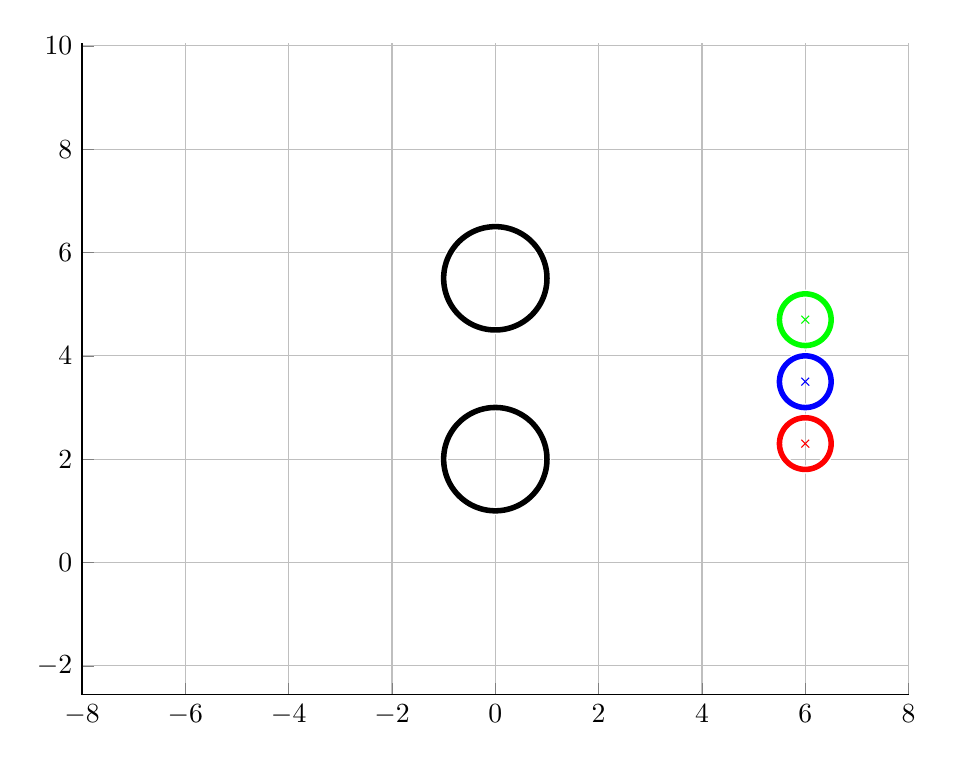
\begin{tikzpicture}

\begin{axis}[%
width=4.133in,
height=3.26in,
at={(0.693in,0.44in)},
scale only axis,
unbounded coords=jump,
xmin=-8,
xmax=8,
xmajorgrids,
ymin=-2.55967741935484,
ymax=10.0596774193548,
ymajorgrids,
axis background/.style={fill=white},
axis x line*=bottom,
axis y line*=left
]
\addplot [color=blue,only marks,mark=x,mark options={solid},forget plot]
  table[row sep=crcr]{%
6	3.5\\
};
\addplot [color=red,only marks,mark=x,mark options={solid},forget plot]
  table[row sep=crcr]{%
6	2.3\\
};
\addplot [color=green,only marks,mark=x,mark options={solid},forget plot]
  table[row sep=crcr]{%
6	4.7\\
};
\addplot [color=white,solid,line width=3.0pt,forget plot]
  table[row sep=crcr]{%
6.49991865139972	3.49900011977623\\
6.49961406490927	3.51644986812748\\
6.49870067652964	3.5338783566483\\
6.49717959908386	3.55126435141006\\
6.49505268577051	3.56858667025627\\
6.49232252790583	3.5858242086097\\
6.48899245176663	3.60295596518511\\
6.48506651453772	3.61996106757607\\
6.48054949936888	3.63681879768473\\
6.4754469095473	3.65350861696371\\
6.46976496179268	3.67001019143907\\
6.46351057868312	3.68630341648419\\
6.45669138022102	3.70236844131413\\
6.44931567454931	3.71818569317077\\
6.44139244782919	3.73373590116918\\
6.43293135329194	3.74900011977623\\
6.42394269947794	3.76395975189283\\
6.41443743767724	3.77859657151161\\
6.4044271485872	3.79289274592247\\
6.39392402820308	3.80683085743906\\
6.38294087295921	3.8203939246195\\
6.37149106413842	3.83356542295566\\
6.35958855156905	3.84632930500573\\
6.34724783662922	3.85867001994556\\
6.33448395457915	3.87057253251493\\
6.32131245624299	3.88202234133572\\
6.30774938906255	3.89300549657959\\
6.29381127754596	3.90350861696371\\
6.2795151031351	3.91351890605375\\
6.26487828351633	3.92302416785445\\
6.24991865139972	3.93201282166845\\
6.23465443279267	3.9404739162057\\
6.21910422479426	3.94839714292582\\
6.20328697293762	3.95577284859753\\
6.18722194810768	3.96259204705963\\
6.17092872306256	3.96884643016919\\
6.1544271485872	3.97452837792381\\
6.13773732930822	3.97963096774539\\
6.12087959919956	3.98414798291423\\
6.1038744968086	3.98807392014314\\
6.08674274023319	3.99140399628234\\
6.06950520187976	3.99413415414702\\
6.05218288303355	3.99626106746037\\
6.03479688827179	3.99778214490614\\
6.01736839975097	3.99869553328578\\
5.99991865139972	3.99900011977623\\
5.98246890304847	3.99869553328578\\
5.96504041452766	3.99778214490614\\
5.9476544197659	3.99626106746037\\
5.93033210091969	3.99413415414702\\
5.91309456256626	3.99140399628234\\
5.89596280599084	3.98807392014314\\
5.87895770359989	3.98414798291423\\
5.86209997349122	3.97963096774539\\
5.84541015421225	3.97452837792381\\
5.82890857973689	3.96884643016919\\
5.81261535469177	3.96259204705963\\
5.79655032986182	3.95577284859753\\
5.78073307800519	3.94839714292582\\
5.76518287000678	3.9404739162057\\
5.74991865139972	3.93201282166845\\
5.73495901928312	3.92302416785445\\
5.72032219966435	3.91351890605375\\
5.70602602525349	3.90350861696371\\
5.69208791373689	3.89300549657959\\
5.67852484655645	3.88202234133572\\
5.66535334822029	3.87057253251493\\
5.65258946617022	3.85867001994556\\
5.6402487512304	3.84632930500573\\
5.62834623866103	3.83356542295566\\
5.61689642984024	3.8203939246195\\
5.60591327459636	3.80683085743906\\
5.59541015421225	3.79289274592247\\
5.5853998651222	3.77859657151161\\
5.57589460332151	3.76395975189283\\
5.5669059495075	3.74900011977623\\
5.55844485497026	3.73373590116918\\
5.55052162825014	3.71818569317077\\
5.54314592257842	3.70236844131413\\
5.53632672411633	3.68630341648419\\
5.53007234100677	3.67001019143907\\
5.52439039325215	3.65350861696371\\
5.51928780343056	3.63681879768473\\
5.51477078826173	3.61996106757607\\
5.51084485103282	3.60295596518511\\
5.50751477489362	3.5858242086097\\
5.50478461702894	3.56858667025627\\
5.50265770371559	3.55126435141006\\
5.50113662626981	3.5338783566483\\
5.50022323789018	3.51644986812748\\
5.49991865139972	3.49900011977623\\
5.50022323789018	3.48155037142498\\
5.50113662626981	3.46412188290417\\
5.50265770371559	3.44673588814241\\
5.50478461702894	3.4294135692962\\
5.50751477489362	3.41217603094277\\
5.51084485103282	3.39504427436735\\
5.51477078826173	3.3780391719764\\
5.51928780343056	3.36118144186773\\
5.52439039325215	3.34449162258876\\
5.53007234100677	3.3279900481134\\
5.53632672411633	3.31169682306828\\
5.54314592257842	3.29563179823833\\
5.55052162825014	3.27981454638169\\
5.55844485497026	3.26426433838329\\
5.5669059495075	3.24900011977623\\
5.57589460332151	3.23404048765963\\
5.5853998651222	3.21940366804086\\
5.59541015421225	3.20510749363\\
5.60591327459636	3.1911693821134\\
5.61689642984023	3.17760631493296\\
5.62834623866103	3.1644348165968\\
5.6402487512304	3.15167093454673\\
5.65258946617022	3.13933021960691\\
5.66535334822029	3.12742770703754\\
5.67852484655645	3.11597789821674\\
5.69208791373689	3.10499474297287\\
5.70602602525349	3.09449162258876\\
5.72032219966435	3.08448133349871\\
5.73495901928312	3.07497607169802\\
5.74991865139972	3.06598741788401\\
5.76518287000678	3.05752632334677\\
5.78073307800519	3.04960309662665\\
5.79655032986182	3.04222739095493\\
5.81261535469177	3.03540819249284\\
5.82890857973689	3.02915380938328\\
5.84541015421225	3.02347186162866\\
5.86209997349122	3.01836927180707\\
5.87895770359989	3.01385225663823\\
5.89596280599084	3.00992631940933\\
5.91309456256626	3.00659624327013\\
5.93033210091969	3.00386608540545\\
5.9476544197659	3.0017391720921\\
5.96504041452766	3.00021809464632\\
5.98246890304847	2.99930470626668\\
5.99991865139972	2.99900011977623\\
6.01736839975097	2.99930470626668\\
6.03479688827179	3.00021809464632\\
6.05218288303355	3.0017391720921\\
6.06950520187976	3.00386608540545\\
6.08674274023319	3.00659624327013\\
6.1038744968086	3.00992631940933\\
6.12087959919956	3.01385225663823\\
6.13773732930822	3.01836927180707\\
6.1544271485872	3.02347186162866\\
6.17092872306256	3.02915380938328\\
6.18722194810768	3.03540819249284\\
6.20328697293762	3.04222739095493\\
6.21910422479426	3.04960309662665\\
6.23465443279267	3.05752632334677\\
6.24991865139972	3.06598741788401\\
6.26487828351633	3.07497607169802\\
6.2795151031351	3.08448133349871\\
6.29381127754596	3.09449162258876\\
6.30774938906255	3.10499474297287\\
6.32131245624299	3.11597789821674\\
6.33448395457915	3.12742770703754\\
6.34724783662922	3.13933021960691\\
6.35958855156905	3.15167093454673\\
6.37149106413842	3.1644348165968\\
6.38294087295921	3.17760631493296\\
6.39392402820308	3.1911693821134\\
6.4044271485872	3.20510749363\\
6.41443743767724	3.21940366804086\\
6.42394269947794	3.23404048765963\\
6.43293135329194	3.24900011977623\\
6.44139244782919	3.26426433838329\\
6.44931567454931	3.27981454638169\\
6.45669138022102	3.29563179823833\\
6.46351057868312	3.31169682306828\\
6.46976496179268	3.3279900481134\\
6.4754469095473	3.34449162258876\\
6.48054949936888	3.36118144186773\\
6.48506651453772	3.3780391719764\\
6.48899245176663	3.39504427436735\\
6.49232252790583	3.41217603094277\\
6.49505268577051	3.4294135692962\\
6.49717959908386	3.44673588814241\\
6.49870067652964	3.46412188290417\\
6.49961406490927	3.48155037142498\\
6.49991865139972	3.49900011977623\\
nan	nan\\
};
\addplot [color=blue,solid,line width=2.0pt,forget plot]
  table[row sep=crcr]{%
6.49991865139972	3.49900011977623\\
6.49961406490927	3.51644986812748\\
6.49870067652964	3.5338783566483\\
6.49717959908386	3.55126435141006\\
6.49505268577051	3.56858667025627\\
6.49232252790583	3.5858242086097\\
6.48899245176663	3.60295596518511\\
6.48506651453772	3.61996106757607\\
6.48054949936888	3.63681879768473\\
6.4754469095473	3.65350861696371\\
6.46976496179268	3.67001019143907\\
6.46351057868312	3.68630341648419\\
6.45669138022102	3.70236844131413\\
6.44931567454931	3.71818569317077\\
6.44139244782919	3.73373590116918\\
6.43293135329194	3.74900011977623\\
6.42394269947794	3.76395975189283\\
6.41443743767724	3.77859657151161\\
6.4044271485872	3.79289274592247\\
6.39392402820308	3.80683085743906\\
6.38294087295921	3.8203939246195\\
6.37149106413842	3.83356542295566\\
6.35958855156905	3.84632930500573\\
6.34724783662922	3.85867001994556\\
6.33448395457915	3.87057253251493\\
6.32131245624299	3.88202234133572\\
6.30774938906255	3.89300549657959\\
6.29381127754596	3.90350861696371\\
6.2795151031351	3.91351890605375\\
6.26487828351633	3.92302416785445\\
6.24991865139972	3.93201282166845\\
6.23465443279267	3.9404739162057\\
6.21910422479426	3.94839714292582\\
6.20328697293762	3.95577284859753\\
6.18722194810768	3.96259204705963\\
6.17092872306256	3.96884643016919\\
6.1544271485872	3.97452837792381\\
6.13773732930822	3.97963096774539\\
6.12087959919956	3.98414798291423\\
6.1038744968086	3.98807392014314\\
6.08674274023319	3.99140399628234\\
6.06950520187976	3.99413415414702\\
6.05218288303355	3.99626106746037\\
6.03479688827179	3.99778214490614\\
6.01736839975097	3.99869553328578\\
5.99991865139972	3.99900011977623\\
5.98246890304847	3.99869553328578\\
5.96504041452766	3.99778214490614\\
5.9476544197659	3.99626106746037\\
5.93033210091969	3.99413415414702\\
5.91309456256626	3.99140399628234\\
5.89596280599084	3.98807392014314\\
5.87895770359989	3.98414798291423\\
5.86209997349122	3.97963096774539\\
5.84541015421225	3.97452837792381\\
5.82890857973689	3.96884643016919\\
5.81261535469177	3.96259204705963\\
5.79655032986182	3.95577284859753\\
5.78073307800519	3.94839714292582\\
5.76518287000678	3.9404739162057\\
5.74991865139972	3.93201282166845\\
5.73495901928312	3.92302416785445\\
5.72032219966435	3.91351890605375\\
5.70602602525349	3.90350861696371\\
5.69208791373689	3.89300549657959\\
5.67852484655645	3.88202234133572\\
5.66535334822029	3.87057253251493\\
5.65258946617022	3.85867001994556\\
5.6402487512304	3.84632930500573\\
5.62834623866103	3.83356542295566\\
5.61689642984024	3.8203939246195\\
5.60591327459636	3.80683085743906\\
5.59541015421225	3.79289274592247\\
5.5853998651222	3.77859657151161\\
5.57589460332151	3.76395975189283\\
5.5669059495075	3.74900011977623\\
5.55844485497026	3.73373590116918\\
5.55052162825014	3.71818569317077\\
5.54314592257842	3.70236844131413\\
5.53632672411633	3.68630341648419\\
5.53007234100677	3.67001019143907\\
5.52439039325215	3.65350861696371\\
5.51928780343056	3.63681879768473\\
5.51477078826173	3.61996106757607\\
5.51084485103282	3.60295596518511\\
5.50751477489362	3.5858242086097\\
5.50478461702894	3.56858667025627\\
5.50265770371559	3.55126435141006\\
5.50113662626981	3.5338783566483\\
5.50022323789018	3.51644986812748\\
5.49991865139972	3.49900011977623\\
5.50022323789018	3.48155037142498\\
5.50113662626981	3.46412188290417\\
5.50265770371559	3.44673588814241\\
5.50478461702894	3.4294135692962\\
5.50751477489362	3.41217603094277\\
5.51084485103282	3.39504427436735\\
5.51477078826173	3.3780391719764\\
5.51928780343056	3.36118144186773\\
5.52439039325215	3.34449162258876\\
5.53007234100677	3.3279900481134\\
5.53632672411633	3.31169682306828\\
5.54314592257842	3.29563179823833\\
5.55052162825014	3.27981454638169\\
5.55844485497026	3.26426433838329\\
5.5669059495075	3.24900011977623\\
5.57589460332151	3.23404048765963\\
5.5853998651222	3.21940366804086\\
5.59541015421225	3.20510749363\\
5.60591327459636	3.1911693821134\\
5.61689642984023	3.17760631493296\\
5.62834623866103	3.1644348165968\\
5.6402487512304	3.15167093454673\\
5.65258946617022	3.13933021960691\\
5.66535334822029	3.12742770703754\\
5.67852484655645	3.11597789821674\\
5.69208791373689	3.10499474297287\\
5.70602602525349	3.09449162258876\\
5.72032219966435	3.08448133349871\\
5.73495901928312	3.07497607169802\\
5.74991865139972	3.06598741788401\\
5.76518287000678	3.05752632334677\\
5.78073307800519	3.04960309662665\\
5.79655032986182	3.04222739095493\\
5.81261535469177	3.03540819249284\\
5.82890857973689	3.02915380938328\\
5.84541015421225	3.02347186162866\\
5.86209997349122	3.01836927180707\\
5.87895770359989	3.01385225663823\\
5.89596280599084	3.00992631940933\\
5.91309456256626	3.00659624327013\\
5.93033210091969	3.00386608540545\\
5.9476544197659	3.0017391720921\\
5.96504041452766	3.00021809464632\\
5.98246890304847	2.99930470626668\\
5.99991865139972	2.99900011977623\\
6.01736839975097	2.99930470626668\\
6.03479688827179	3.00021809464632\\
6.05218288303355	3.0017391720921\\
6.06950520187976	3.00386608540545\\
6.08674274023319	3.00659624327013\\
6.1038744968086	3.00992631940933\\
6.12087959919956	3.01385225663823\\
6.13773732930822	3.01836927180707\\
6.1544271485872	3.02347186162866\\
6.17092872306256	3.02915380938328\\
6.18722194810768	3.03540819249284\\
6.20328697293762	3.04222739095493\\
6.21910422479426	3.04960309662665\\
6.23465443279267	3.05752632334677\\
6.24991865139972	3.06598741788401\\
6.26487828351633	3.07497607169802\\
6.2795151031351	3.08448133349871\\
6.29381127754596	3.09449162258876\\
6.30774938906255	3.10499474297287\\
6.32131245624299	3.11597789821674\\
6.33448395457915	3.12742770703754\\
6.34724783662922	3.13933021960691\\
6.35958855156905	3.15167093454673\\
6.37149106413842	3.1644348165968\\
6.38294087295921	3.17760631493296\\
6.39392402820308	3.1911693821134\\
6.4044271485872	3.20510749363\\
6.41443743767724	3.21940366804086\\
6.42394269947794	3.23404048765963\\
6.43293135329194	3.24900011977623\\
6.44139244782919	3.26426433838329\\
6.44931567454931	3.27981454638169\\
6.45669138022102	3.29563179823833\\
6.46351057868312	3.31169682306828\\
6.46976496179268	3.3279900481134\\
6.4754469095473	3.34449162258876\\
6.48054949936888	3.36118144186773\\
6.48506651453772	3.3780391719764\\
6.48899245176663	3.39504427436735\\
6.49232252790583	3.41217603094277\\
6.49505268577051	3.4294135692962\\
6.49717959908386	3.44673588814241\\
6.49870067652964	3.46412188290417\\
6.49961406490927	3.48155037142498\\
6.49991865139972	3.49900011977623\\
nan	nan\\
};
\addplot [color=white,solid,line width=3.0pt,forget plot]
  table[row sep=crcr]{%
6.50014722519847	2.30100001361806\\
6.49984263870802	2.31844976196931\\
6.49892925032838	2.33587825049012\\
6.49740817288261	2.35326424525189\\
6.49528125956926	2.37058656409809\\
6.49255110170458	2.38782410245152\\
6.48922102556537	2.40495585902694\\
6.48529508833647	2.42196096141789\\
6.48077807316763	2.43881869152656\\
6.47567548334605	2.45550851080553\\
6.46999353559143	2.47201008528089\\
6.46373915248187	2.48830331032602\\
6.45691995401977	2.50436833515596\\
6.44954424834806	2.5201855870126\\
6.44162102162793	2.53573579501101\\
6.43315992709069	2.55100001361806\\
6.42417127327668	2.56595964573466\\
6.41466601147599	2.58059646535343\\
6.40465572238594	2.5948926397643\\
6.39415260200183	2.60883075128089\\
6.38316944675796	2.62239381846133\\
6.37171963793717	2.63556531679749\\
6.3598171253678	2.64832919884756\\
6.34747641042797	2.66066991378739\\
6.3347125283779	2.67257242635676\\
6.32154103004174	2.68402223517755\\
6.3079779628613	2.69500539042142\\
6.29403985134471	2.70550851080553\\
6.27974367693384	2.71551879989558\\
6.26510685731507	2.72502406169627\\
6.25014722519847	2.73401271551028\\
6.23488300659142	2.74247381004752\\
6.21933279859301	2.75039703676764\\
6.20351554673637	2.75777274243936\\
6.18745052190643	2.76459194090145\\
6.17115729686131	2.77084632401101\\
6.15465572238594	2.77652827176564\\
6.13796590310697	2.78163086158722\\
6.12110817299831	2.78614787675606\\
6.10410307060735	2.79007381398496\\
6.08697131403194	2.79340389012416\\
6.0697337756785	2.79613404798884\\
6.0524114568323	2.7982609613022\\
6.03502546207053	2.79978203874797\\
6.01759697354972	2.80069542712761\\
6.00014722519847	2.80100001361806\\
5.98269747684722	2.80069542712761\\
5.96526898832641	2.79978203874797\\
5.94788299356464	2.7982609613022\\
5.93056067471844	2.79613404798884\\
5.91332313636501	2.79340389012416\\
5.89619137978959	2.79007381398496\\
5.87918627739864	2.78614787675606\\
5.86232854728997	2.78163086158722\\
5.845638728011	2.77652827176564\\
5.82913715353564	2.77084632401101\\
5.81284392849052	2.76459194090145\\
5.79677890366057	2.75777274243936\\
5.78096165180393	2.75039703676764\\
5.76541144380553	2.74247381004752\\
5.75014722519847	2.73401271551028\\
5.73518759308187	2.72502406169627\\
5.7205507734631	2.71551879989558\\
5.70625459905223	2.70550851080553\\
5.69231648753564	2.69500539042142\\
5.6787534203552	2.68402223517755\\
5.66558192201904	2.67257242635676\\
5.65281803996897	2.66066991378739\\
5.64047732502915	2.64832919884756\\
5.62857481245977	2.63556531679749\\
5.61712500363898	2.62239381846133\\
5.60614184839511	2.60883075128089\\
5.595638728011	2.5948926397643\\
5.58562843892095	2.58059646535343\\
5.57612317712026	2.56595964573466\\
5.56713452330625	2.55100001361806\\
5.55867342876901	2.53573579501101\\
5.55075020204889	2.5201855870126\\
5.54337449637717	2.50436833515596\\
5.53655529791508	2.48830331032602\\
5.53030091480552	2.47201008528089\\
5.52461896705089	2.45550851080553\\
5.51951637722931	2.43881869152656\\
5.51499936206047	2.42196096141789\\
5.51107342483157	2.40495585902694\\
5.50774334869237	2.38782410245152\\
5.50501319082769	2.37058656409809\\
5.50288627751434	2.35326424525189\\
5.50136520006856	2.33587825049012\\
5.50045181168892	2.31844976196931\\
5.50014722519847	2.30100001361806\\
5.50045181168892	2.28355026526681\\
5.50136520006856	2.266121776746\\
5.50288627751434	2.24873578198423\\
5.50501319082769	2.23141346313803\\
5.50774334869237	2.21417592478459\\
5.51107342483157	2.19704416820918\\
5.51499936206047	2.18003906581823\\
5.51951637722931	2.16318133570956\\
5.52461896705089	2.14649151643059\\
5.53030091480552	2.12998994195523\\
5.53655529791508	2.1136967169101\\
5.54337449637717	2.09763169208016\\
5.55075020204889	2.08181444022352\\
5.55867342876901	2.06626423222511\\
5.56713452330625	2.05100001361806\\
5.57612317712026	2.03604038150146\\
5.58562843892095	2.02140356188269\\
5.595638728011	2.00710738747182\\
5.60614184839511	1.99316927595523\\
5.61712500363898	1.97960620877479\\
5.62857481245977	1.96643471043863\\
5.64047732502915	1.95367082838856\\
5.65281803996897	1.94133011344873\\
5.66558192201904	1.92942760087936\\
5.6787534203552	1.91797779205857\\
5.69231648753564	1.9069946368147\\
5.70625459905223	1.89649151643059\\
5.7205507734631	1.88648122734054\\
5.73518759308187	1.87697596553985\\
5.75014722519847	1.86798731172584\\
5.76541144380553	1.8595262171886\\
5.78096165180393	1.85160299046848\\
5.79677890366057	1.84422728479676\\
5.81284392849052	1.83740808633467\\
5.82913715353564	1.83115370322511\\
5.845638728011	1.82547175547048\\
5.86232854728997	1.8203691656489\\
5.87918627739864	1.81585215048006\\
5.89619137978959	1.81192621325116\\
5.91332313636501	1.80859613711196\\
5.93056067471844	1.80586597924727\\
5.94788299356464	1.80373906593392\\
5.96526898832641	1.80221798848815\\
5.98269747684722	1.80130460010851\\
6.00014722519847	1.80100001361806\\
6.01759697354972	1.80130460010851\\
6.03502546207053	1.80221798848815\\
6.0524114568323	1.80373906593392\\
6.0697337756785	1.80586597924727\\
6.08697131403194	1.80859613711196\\
6.10410307060735	1.81192621325116\\
6.12110817299831	1.81585215048006\\
6.13796590310697	1.8203691656489\\
6.15465572238594	1.82547175547048\\
6.17115729686131	1.83115370322511\\
6.18745052190643	1.83740808633467\\
6.20351554673637	1.84422728479676\\
6.21933279859301	1.85160299046848\\
6.23488300659142	1.8595262171886\\
6.25014722519847	1.86798731172584\\
6.26510685731507	1.87697596553985\\
6.27974367693384	1.88648122734054\\
6.29403985134471	1.89649151643059\\
6.3079779628613	1.9069946368147\\
6.32154103004174	1.91797779205857\\
6.3347125283779	1.92942760087936\\
6.34747641042797	1.94133011344873\\
6.3598171253678	1.95367082838856\\
6.37171963793717	1.96643471043863\\
6.38316944675796	1.97960620877479\\
6.39415260200183	1.99316927595523\\
6.40465572238594	2.00710738747182\\
6.41466601147599	2.02140356188269\\
6.42417127327668	2.03604038150146\\
6.43315992709069	2.05100001361806\\
6.44162102162793	2.06626423222511\\
6.44954424834806	2.08181444022352\\
6.45691995401977	2.09763169208016\\
6.46373915248186	2.1136967169101\\
6.46999353559143	2.12998994195523\\
6.47567548334605	2.14649151643059\\
6.48077807316763	2.16318133570956\\
6.48529508833647	2.18003906581823\\
6.48922102556537	2.19704416820918\\
6.49255110170458	2.21417592478459\\
6.49528125956926	2.23141346313803\\
6.49740817288261	2.24873578198423\\
6.49892925032838	2.266121776746\\
6.49984263870802	2.28355026526681\\
6.50014722519847	2.30100001361806\\
nan	nan\\
};
\addplot [color=red,solid,line width=2.0pt,forget plot]
  table[row sep=crcr]{%
6.50014722519847	2.30100001361806\\
6.49984263870802	2.31844976196931\\
6.49892925032838	2.33587825049012\\
6.49740817288261	2.35326424525189\\
6.49528125956926	2.37058656409809\\
6.49255110170458	2.38782410245152\\
6.48922102556537	2.40495585902694\\
6.48529508833647	2.42196096141789\\
6.48077807316763	2.43881869152656\\
6.47567548334605	2.45550851080553\\
6.46999353559143	2.47201008528089\\
6.46373915248187	2.48830331032602\\
6.45691995401977	2.50436833515596\\
6.44954424834806	2.5201855870126\\
6.44162102162793	2.53573579501101\\
6.43315992709069	2.55100001361806\\
6.42417127327668	2.56595964573466\\
6.41466601147599	2.58059646535343\\
6.40465572238594	2.5948926397643\\
6.39415260200183	2.60883075128089\\
6.38316944675796	2.62239381846133\\
6.37171963793717	2.63556531679749\\
6.3598171253678	2.64832919884756\\
6.34747641042797	2.66066991378739\\
6.3347125283779	2.67257242635676\\
6.32154103004174	2.68402223517755\\
6.3079779628613	2.69500539042142\\
6.29403985134471	2.70550851080553\\
6.27974367693384	2.71551879989558\\
6.26510685731507	2.72502406169627\\
6.25014722519847	2.73401271551028\\
6.23488300659142	2.74247381004752\\
6.21933279859301	2.75039703676764\\
6.20351554673637	2.75777274243936\\
6.18745052190643	2.76459194090145\\
6.17115729686131	2.77084632401101\\
6.15465572238594	2.77652827176564\\
6.13796590310697	2.78163086158722\\
6.12110817299831	2.78614787675606\\
6.10410307060735	2.79007381398496\\
6.08697131403194	2.79340389012416\\
6.0697337756785	2.79613404798884\\
6.0524114568323	2.7982609613022\\
6.03502546207053	2.79978203874797\\
6.01759697354972	2.80069542712761\\
6.00014722519847	2.80100001361806\\
5.98269747684722	2.80069542712761\\
5.96526898832641	2.79978203874797\\
5.94788299356464	2.7982609613022\\
5.93056067471844	2.79613404798884\\
5.91332313636501	2.79340389012416\\
5.89619137978959	2.79007381398496\\
5.87918627739864	2.78614787675606\\
5.86232854728997	2.78163086158722\\
5.845638728011	2.77652827176564\\
5.82913715353564	2.77084632401101\\
5.81284392849052	2.76459194090145\\
5.79677890366057	2.75777274243936\\
5.78096165180393	2.75039703676764\\
5.76541144380553	2.74247381004752\\
5.75014722519847	2.73401271551028\\
5.73518759308187	2.72502406169627\\
5.7205507734631	2.71551879989558\\
5.70625459905223	2.70550851080553\\
5.69231648753564	2.69500539042142\\
5.6787534203552	2.68402223517755\\
5.66558192201904	2.67257242635676\\
5.65281803996897	2.66066991378739\\
5.64047732502915	2.64832919884756\\
5.62857481245977	2.63556531679749\\
5.61712500363898	2.62239381846133\\
5.60614184839511	2.60883075128089\\
5.595638728011	2.5948926397643\\
5.58562843892095	2.58059646535343\\
5.57612317712026	2.56595964573466\\
5.56713452330625	2.55100001361806\\
5.55867342876901	2.53573579501101\\
5.55075020204889	2.5201855870126\\
5.54337449637717	2.50436833515596\\
5.53655529791508	2.48830331032602\\
5.53030091480552	2.47201008528089\\
5.52461896705089	2.45550851080553\\
5.51951637722931	2.43881869152656\\
5.51499936206047	2.42196096141789\\
5.51107342483157	2.40495585902694\\
5.50774334869237	2.38782410245152\\
5.50501319082769	2.37058656409809\\
5.50288627751434	2.35326424525189\\
5.50136520006856	2.33587825049012\\
5.50045181168892	2.31844976196931\\
5.50014722519847	2.30100001361806\\
5.50045181168892	2.28355026526681\\
5.50136520006856	2.266121776746\\
5.50288627751434	2.24873578198423\\
5.50501319082769	2.23141346313803\\
5.50774334869237	2.21417592478459\\
5.51107342483157	2.19704416820918\\
5.51499936206047	2.18003906581823\\
5.51951637722931	2.16318133570956\\
5.52461896705089	2.14649151643059\\
5.53030091480552	2.12998994195523\\
5.53655529791508	2.1136967169101\\
5.54337449637717	2.09763169208016\\
5.55075020204889	2.08181444022352\\
5.55867342876901	2.06626423222511\\
5.56713452330625	2.05100001361806\\
5.57612317712026	2.03604038150146\\
5.58562843892095	2.02140356188269\\
5.595638728011	2.00710738747182\\
5.60614184839511	1.99316927595523\\
5.61712500363898	1.97960620877479\\
5.62857481245977	1.96643471043863\\
5.64047732502915	1.95367082838856\\
5.65281803996897	1.94133011344873\\
5.66558192201904	1.92942760087936\\
5.6787534203552	1.91797779205857\\
5.69231648753564	1.9069946368147\\
5.70625459905223	1.89649151643059\\
5.7205507734631	1.88648122734054\\
5.73518759308187	1.87697596553985\\
5.75014722519847	1.86798731172584\\
5.76541144380553	1.8595262171886\\
5.78096165180393	1.85160299046848\\
5.79677890366057	1.84422728479676\\
5.81284392849052	1.83740808633467\\
5.82913715353564	1.83115370322511\\
5.845638728011	1.82547175547048\\
5.86232854728997	1.8203691656489\\
5.87918627739864	1.81585215048006\\
5.89619137978959	1.81192621325116\\
5.91332313636501	1.80859613711196\\
5.93056067471844	1.80586597924727\\
5.94788299356464	1.80373906593392\\
5.96526898832641	1.80221798848815\\
5.98269747684722	1.80130460010851\\
6.00014722519847	1.80100001361806\\
6.01759697354972	1.80130460010851\\
6.03502546207053	1.80221798848815\\
6.0524114568323	1.80373906593392\\
6.0697337756785	1.80586597924727\\
6.08697131403194	1.80859613711196\\
6.10410307060735	1.81192621325116\\
6.12110817299831	1.81585215048006\\
6.13796590310697	1.8203691656489\\
6.15465572238594	1.82547175547048\\
6.17115729686131	1.83115370322511\\
6.18745052190643	1.83740808633467\\
6.20351554673637	1.84422728479676\\
6.21933279859301	1.85160299046848\\
6.23488300659142	1.8595262171886\\
6.25014722519847	1.86798731172584\\
6.26510685731507	1.87697596553985\\
6.27974367693384	1.88648122734054\\
6.29403985134471	1.89649151643059\\
6.3079779628613	1.9069946368147\\
6.32154103004174	1.91797779205857\\
6.3347125283779	1.92942760087936\\
6.34747641042797	1.94133011344873\\
6.3598171253678	1.95367082838856\\
6.37171963793717	1.96643471043863\\
6.38316944675796	1.97960620877479\\
6.39415260200183	1.99316927595523\\
6.40465572238594	2.00710738747182\\
6.41466601147599	2.02140356188269\\
6.42417127327668	2.03604038150146\\
6.43315992709069	2.05100001361806\\
6.44162102162793	2.06626423222511\\
6.44954424834806	2.08181444022352\\
6.45691995401977	2.09763169208016\\
6.46373915248186	2.1136967169101\\
6.46999353559143	2.12998994195523\\
6.47567548334605	2.14649151643059\\
6.48077807316763	2.16318133570956\\
6.48529508833647	2.18003906581823\\
6.48922102556537	2.19704416820918\\
6.49255110170458	2.21417592478459\\
6.49528125956926	2.23141346313803\\
6.49740817288261	2.24873578198423\\
6.49892925032838	2.266121776746\\
6.49984263870802	2.28355026526681\\
6.50014722519847	2.30100001361806\\
nan	nan\\
};
\addplot [color=white,solid,line width=3.0pt,forget plot]
  table[row sep=crcr]{%
6.50003462748056	4.69899999525176\\
6.49973004099011	4.71644974360301\\
6.49881665261047	4.73387823212382\\
6.49729557516469	4.75126422688559\\
6.49516866185134	4.76858654573179\\
6.49243850398666	4.78582408408523\\
6.48910842784746	4.80295584066064\\
6.48518249061856	4.81996094305159\\
6.48066547544972	4.83681867316026\\
6.47556288562813	4.85350849243923\\
6.46988093787351	4.8700100669146\\
6.46362655476395	4.88630329195972\\
6.45680735630186	4.90236831678966\\
6.44943165063014	4.9181855686463\\
6.44150842391002	4.93373577664471\\
6.43304732937278	4.94899999525176\\
6.42405867555877	4.96395962736836\\
6.41455341375808	4.97859644698713\\
6.40454312466803	4.992892621398\\
6.39404000428392	5.00683073291459\\
6.38305684904005	5.02039380009503\\
6.37160704021925	5.03356529843119\\
6.35970452764988	5.04632918048126\\
6.34736381271006	5.05866989542109\\
6.33459993065999	5.07057240799046\\
6.32142843232383	5.08202221681125\\
6.30786536514339	5.09300537205512\\
6.29392725362679	5.10350849243923\\
6.27963107921593	5.11351878152928\\
6.26499425959716	5.12302404332997\\
6.25003462748056	5.13201269714398\\
6.2347704088735	5.14047379168122\\
6.2192202008751	5.14839701840134\\
6.20340294901846	5.15577272407306\\
6.18733792418851	5.16259192253515\\
6.17104469914339	5.16884630564472\\
6.15454312466803	5.17452825339934\\
6.13785330538906	5.17963084322092\\
6.12099557528039	5.18414785838976\\
6.10399047288944	5.18807379561866\\
6.08685871631402	5.19140387175786\\
6.06962117796059	5.19413402962255\\
6.05229885911438	5.1962609429359\\
6.03491286435262	5.19778202038167\\
6.01748437583181	5.19869540876131\\
6.00003462748056	5.19899999525176\\
5.98258487912931	5.19869540876131\\
5.9651563906085	5.19778202038167\\
5.94777039584673	5.1962609429359\\
5.93044807700053	5.19413402962255\\
5.91321053864709	5.19140387175786\\
5.89607878207168	5.18807379561866\\
5.87907367968072	5.18414785838976\\
5.86221594957206	5.17963084322092\\
5.84552613029308	5.17452825339934\\
5.82902455581772	5.16884630564472\\
5.8127313307726	5.16259192253515\\
5.79666630594266	5.15577272407306\\
5.78084905408602	5.14839701840134\\
5.76529884608761	5.14047379168122\\
5.75003462748056	5.13201269714398\\
5.73507499536395	5.12302404332997\\
5.72043817574518	5.11351878152928\\
5.70614200133432	5.10350849243923\\
5.69220388981773	5.09300537205512\\
5.67864082263729	5.08202221681125\\
5.66546932430113	5.07057240799046\\
5.65270544225106	5.05866989542109\\
5.64036472731123	5.04632918048126\\
5.62846221474186	5.03356529843119\\
5.61701240592107	5.02039380009503\\
5.6060292506772	5.00683073291459\\
5.59552613029308	4.992892621398\\
5.58551584120304	4.97859644698713\\
5.57601057940234	4.96395962736836\\
5.56702192558834	4.94899999525176\\
5.55856083105109	4.93373577664471\\
5.55063760433097	4.9181855686463\\
5.54326189865926	4.90236831678966\\
5.53644270019716	4.88630329195972\\
5.5301883170876	4.8700100669146\\
5.52450636933298	4.85350849243923\\
5.5194037795114	4.83681867316026\\
5.51488676434256	4.81996094305159\\
5.51096082711365	4.80295584066064\\
5.50763075097445	4.78582408408523\\
5.50490059310977	4.76858654573179\\
5.50277367979642	4.75126422688559\\
5.50125260235065	4.73387823212382\\
5.50033921397101	4.71644974360301\\
5.50003462748056	4.69899999525176\\
5.50033921397101	4.68155024690051\\
5.50125260235065	4.6641217583797\\
5.50277367979642	4.64673576361793\\
5.50490059310977	4.62941344477173\\
5.50763075097445	4.6121759064183\\
5.51096082711365	4.59504414984288\\
5.51488676434256	4.57803904745193\\
5.5194037795114	4.56118131734326\\
5.52450636933298	4.54449149806429\\
5.5301883170876	4.52798992358893\\
5.53644270019716	4.5116966985438\\
5.54326189865926	4.49563167371386\\
5.55063760433097	4.47981442185722\\
5.55856083105109	4.46426421385882\\
5.56702192558834	4.44899999525176\\
5.57601057940234	4.43404036313516\\
5.58551584120304	4.41940354351639\\
5.59552613029308	4.40510736910552\\
5.6060292506772	4.39116925758893\\
5.61701240592107	4.37760619040849\\
5.62846221474186	4.36443469207233\\
5.64036472731123	4.35167081002226\\
5.65270544225106	4.33933009508244\\
5.66546932430113	4.32742758251306\\
5.67864082263729	4.31597777369227\\
5.69220388981773	4.3049946184484\\
5.70614200133432	4.29449149806429\\
5.72043817574518	4.28448120897424\\
5.73507499536395	4.27497594717355\\
5.75003462748056	4.26598729335954\\
5.76529884608761	4.2575261988223\\
5.78084905408602	4.24960297210218\\
5.79666630594266	4.24222726643046\\
5.8127313307726	4.23540806796837\\
5.82902455581772	4.22915368485881\\
5.84552613029308	4.22347173710418\\
5.86221594957206	4.2183691472826\\
5.87907367968072	4.21385213211376\\
5.89607878207168	4.20992619488486\\
5.91321053864709	4.20659611874566\\
5.93044807700053	4.20386596088098\\
5.94777039584673	4.20173904756762\\
5.9651563906085	4.20021797012185\\
5.98258487912931	4.19930458174221\\
6.00003462748056	4.19899999525176\\
6.01748437583181	4.19930458174221\\
6.03491286435262	4.20021797012185\\
6.05229885911438	4.20173904756762\\
6.06962117796059	4.20386596088098\\
6.08685871631402	4.20659611874566\\
6.10399047288944	4.20992619488486\\
6.12099557528039	4.21385213211376\\
6.13785330538906	4.2183691472826\\
6.15454312466803	4.22347173710418\\
6.17104469914339	4.22915368485881\\
6.18733792418851	4.23540806796837\\
6.20340294901846	4.24222726643046\\
6.2192202008751	4.24960297210218\\
6.2347704088735	4.2575261988223\\
6.25003462748056	4.26598729335954\\
6.26499425959716	4.27497594717355\\
6.27963107921593	4.28448120897424\\
6.29392725362679	4.29449149806429\\
6.30786536514339	4.3049946184484\\
6.32142843232383	4.31597777369227\\
6.33459993065999	4.32742758251306\\
6.34736381271006	4.33933009508243\\
6.35970452764988	4.35167081002226\\
6.37160704021925	4.36443469207233\\
6.38305684904005	4.37760619040849\\
6.39404000428392	4.39116925758893\\
6.40454312466803	4.40510736910552\\
6.41455341375808	4.41940354351639\\
6.42405867555877	4.43404036313516\\
6.43304732937278	4.44899999525176\\
6.44150842391002	4.46426421385882\\
6.44943165063014	4.47981442185722\\
6.45680735630186	4.49563167371386\\
6.46362655476395	4.5116966985438\\
6.46988093787351	4.52798992358893\\
6.47556288562813	4.54449149806429\\
6.48066547544972	4.56118131734326\\
6.48518249061856	4.57803904745193\\
6.48910842784746	4.59504414984288\\
6.49243850398666	4.61217590641829\\
6.49516866185134	4.62941344477173\\
6.49729557516469	4.64673576361793\\
6.49881665261047	4.6641217583797\\
6.49973004099011	4.68155024690051\\
6.50003462748056	4.69899999525176\\
nan	nan\\
};
\addplot [color=green,solid,line width=2.0pt,forget plot]
  table[row sep=crcr]{%
6.50003462748056	4.69899999525176\\
6.49973004099011	4.71644974360301\\
6.49881665261047	4.73387823212382\\
6.49729557516469	4.75126422688559\\
6.49516866185134	4.76858654573179\\
6.49243850398666	4.78582408408523\\
6.48910842784746	4.80295584066064\\
6.48518249061856	4.81996094305159\\
6.48066547544972	4.83681867316026\\
6.47556288562813	4.85350849243923\\
6.46988093787351	4.8700100669146\\
6.46362655476395	4.88630329195972\\
6.45680735630186	4.90236831678966\\
6.44943165063014	4.9181855686463\\
6.44150842391002	4.93373577664471\\
6.43304732937278	4.94899999525176\\
6.42405867555877	4.96395962736836\\
6.41455341375808	4.97859644698713\\
6.40454312466803	4.992892621398\\
6.39404000428392	5.00683073291459\\
6.38305684904005	5.02039380009503\\
6.37160704021925	5.03356529843119\\
6.35970452764988	5.04632918048126\\
6.34736381271006	5.05866989542109\\
6.33459993065999	5.07057240799046\\
6.32142843232383	5.08202221681125\\
6.30786536514339	5.09300537205512\\
6.29392725362679	5.10350849243923\\
6.27963107921593	5.11351878152928\\
6.26499425959716	5.12302404332997\\
6.25003462748056	5.13201269714398\\
6.2347704088735	5.14047379168122\\
6.2192202008751	5.14839701840134\\
6.20340294901846	5.15577272407306\\
6.18733792418851	5.16259192253515\\
6.17104469914339	5.16884630564472\\
6.15454312466803	5.17452825339934\\
6.13785330538906	5.17963084322092\\
6.12099557528039	5.18414785838976\\
6.10399047288944	5.18807379561866\\
6.08685871631402	5.19140387175786\\
6.06962117796059	5.19413402962255\\
6.05229885911438	5.1962609429359\\
6.03491286435262	5.19778202038167\\
6.01748437583181	5.19869540876131\\
6.00003462748056	5.19899999525176\\
5.98258487912931	5.19869540876131\\
5.9651563906085	5.19778202038167\\
5.94777039584673	5.1962609429359\\
5.93044807700053	5.19413402962255\\
5.91321053864709	5.19140387175786\\
5.89607878207168	5.18807379561866\\
5.87907367968072	5.18414785838976\\
5.86221594957206	5.17963084322092\\
5.84552613029308	5.17452825339934\\
5.82902455581772	5.16884630564472\\
5.8127313307726	5.16259192253515\\
5.79666630594266	5.15577272407306\\
5.78084905408602	5.14839701840134\\
5.76529884608761	5.14047379168122\\
5.75003462748056	5.13201269714398\\
5.73507499536395	5.12302404332997\\
5.72043817574518	5.11351878152928\\
5.70614200133432	5.10350849243923\\
5.69220388981773	5.09300537205512\\
5.67864082263729	5.08202221681125\\
5.66546932430113	5.07057240799046\\
5.65270544225106	5.05866989542109\\
5.64036472731123	5.04632918048126\\
5.62846221474186	5.03356529843119\\
5.61701240592107	5.02039380009503\\
5.6060292506772	5.00683073291459\\
5.59552613029308	4.992892621398\\
5.58551584120304	4.97859644698713\\
5.57601057940234	4.96395962736836\\
5.56702192558834	4.94899999525176\\
5.55856083105109	4.93373577664471\\
5.55063760433097	4.9181855686463\\
5.54326189865926	4.90236831678966\\
5.53644270019716	4.88630329195972\\
5.5301883170876	4.8700100669146\\
5.52450636933298	4.85350849243923\\
5.5194037795114	4.83681867316026\\
5.51488676434256	4.81996094305159\\
5.51096082711365	4.80295584066064\\
5.50763075097445	4.78582408408523\\
5.50490059310977	4.76858654573179\\
5.50277367979642	4.75126422688559\\
5.50125260235065	4.73387823212382\\
5.50033921397101	4.71644974360301\\
5.50003462748056	4.69899999525176\\
5.50033921397101	4.68155024690051\\
5.50125260235065	4.6641217583797\\
5.50277367979642	4.64673576361793\\
5.50490059310977	4.62941344477173\\
5.50763075097445	4.6121759064183\\
5.51096082711365	4.59504414984288\\
5.51488676434256	4.57803904745193\\
5.5194037795114	4.56118131734326\\
5.52450636933298	4.54449149806429\\
5.5301883170876	4.52798992358893\\
5.53644270019716	4.5116966985438\\
5.54326189865926	4.49563167371386\\
5.55063760433097	4.47981442185722\\
5.55856083105109	4.46426421385882\\
5.56702192558834	4.44899999525176\\
5.57601057940234	4.43404036313516\\
5.58551584120304	4.41940354351639\\
5.59552613029308	4.40510736910552\\
5.6060292506772	4.39116925758893\\
5.61701240592107	4.37760619040849\\
5.62846221474186	4.36443469207233\\
5.64036472731123	4.35167081002226\\
5.65270544225106	4.33933009508244\\
5.66546932430113	4.32742758251306\\
5.67864082263729	4.31597777369227\\
5.69220388981773	4.3049946184484\\
5.70614200133432	4.29449149806429\\
5.72043817574518	4.28448120897424\\
5.73507499536395	4.27497594717355\\
5.75003462748056	4.26598729335954\\
5.76529884608761	4.2575261988223\\
5.78084905408602	4.24960297210218\\
5.79666630594266	4.24222726643046\\
5.8127313307726	4.23540806796837\\
5.82902455581772	4.22915368485881\\
5.84552613029308	4.22347173710418\\
5.86221594957206	4.2183691472826\\
5.87907367968072	4.21385213211376\\
5.89607878207168	4.20992619488486\\
5.91321053864709	4.20659611874566\\
5.93044807700053	4.20386596088098\\
5.94777039584673	4.20173904756762\\
5.9651563906085	4.20021797012185\\
5.98258487912931	4.19930458174221\\
6.00003462748056	4.19899999525176\\
6.01748437583181	4.19930458174221\\
6.03491286435262	4.20021797012185\\
6.05229885911438	4.20173904756762\\
6.06962117796059	4.20386596088098\\
6.08685871631402	4.20659611874566\\
6.10399047288944	4.20992619488486\\
6.12099557528039	4.21385213211376\\
6.13785330538906	4.2183691472826\\
6.15454312466803	4.22347173710418\\
6.17104469914339	4.22915368485881\\
6.18733792418851	4.23540806796837\\
6.20340294901846	4.24222726643046\\
6.2192202008751	4.24960297210218\\
6.2347704088735	4.2575261988223\\
6.25003462748056	4.26598729335954\\
6.26499425959716	4.27497594717355\\
6.27963107921593	4.28448120897424\\
6.29392725362679	4.29449149806429\\
6.30786536514339	4.3049946184484\\
6.32142843232383	4.31597777369227\\
6.33459993065999	4.32742758251306\\
6.34736381271006	4.33933009508243\\
6.35970452764988	4.35167081002226\\
6.37160704021925	4.36443469207233\\
6.38305684904005	4.37760619040849\\
6.39404000428392	4.39116925758893\\
6.40454312466803	4.40510736910552\\
6.41455341375808	4.41940354351639\\
6.42405867555877	4.43404036313516\\
6.43304732937278	4.44899999525176\\
6.44150842391002	4.46426421385882\\
6.44943165063014	4.47981442185722\\
6.45680735630186	4.49563167371386\\
6.46362655476395	4.5116966985438\\
6.46988093787351	4.52798992358893\\
6.47556288562813	4.54449149806429\\
6.48066547544972	4.56118131734326\\
6.48518249061856	4.57803904745193\\
6.48910842784746	4.59504414984288\\
6.49243850398666	4.61217590641829\\
6.49516866185134	4.62941344477173\\
6.49729557516469	4.64673576361793\\
6.49881665261047	4.6641217583797\\
6.49973004099011	4.68155024690051\\
6.50003462748056	4.69899999525176\\
nan	nan\\
};
\addplot [color=white,solid,line width=3.0pt,forget plot]
  table[row sep=crcr]{%
1	2\\
0.999390827019096	2.0348994967025\\
0.997564050259824	2.06975647374413\\
0.994521895368273	2.10452846326765\\
0.99026806874157	2.13917310096007\\
0.984807753012208	2.17364817766693\\
0.978147600733806	2.20791169081776\\
0.970295726275996	2.24192189559967\\
0.961261695938319	2.275637355817\\
0.951056516295154	2.30901699437495\\
0.939692620785908	2.34202014332567\\
0.927183854566787	2.37460659341591\\
0.913545457642601	2.4067366430758\\
0.898794046299167	2.43837114678908\\
0.882947592858927	2.46947156278589\\
0.866025403784439	2.5\\
0.848048096156426	2.5299192642332\\
0.829037572555042	2.55919290347075\\
0.809016994374947	2.58778525229247\\
0.788010753606722	2.61566147532566\\
0.766044443118978	2.64278760968654\\
0.743144825477394	2.66913060635886\\
0.719339800338651	2.694658370459\\
0.694658370458997	2.71933980033865\\
0.669130606358858	2.74314482547739\\
0.642787609686539	2.76604444311898\\
0.615661475325658	2.78801075360672\\
0.587785252292473	2.80901699437495\\
0.559192903470747	2.82903757255504\\
0.529919264233205	2.84804809615643\\
0.5	2.86602540378444\\
0.469471562785891	2.88294759285893\\
0.438371146789077	2.89879404629917\\
0.4067366430758	2.9135454576426\\
0.374606593415912	2.92718385456679\\
0.342020143325669	2.93969262078591\\
0.309016994374947	2.95105651629515\\
0.275637355816999	2.96126169593832\\
0.241921895599668	2.970295726276\\
0.207911690817759	2.97814760073381\\
0.17364817766693	2.98480775301221\\
0.139173100960066	2.99026806874157\\
0.104528463267653	2.99452189536827\\
0.0697564737441255	2.99756405025982\\
0.0348994967025011	2.9993908270191\\
6.12323399573677e-17	3\\
-0.0348994967025007	2.9993908270191\\
-0.0697564737441253	2.99756405025982\\
-0.104528463267653	2.99452189536827\\
-0.139173100960065	2.99026806874157\\
-0.17364817766693	2.98480775301221\\
-0.207911690817759	2.97814760073381\\
-0.241921895599668	2.970295726276\\
-0.275637355816999	2.96126169593832\\
-0.309016994374947	2.95105651629515\\
-0.342020143325669	2.93969262078591\\
-0.374606593415912	2.92718385456679\\
-0.4067366430758	2.9135454576426\\
-0.438371146789078	2.89879404629917\\
-0.469471562785891	2.88294759285893\\
-0.5	2.86602540378444\\
-0.529919264233205	2.84804809615643\\
-0.559192903470747	2.82903757255504\\
-0.587785252292473	2.80901699437495\\
-0.615661475325658	2.78801075360672\\
-0.642787609686539	2.76604444311898\\
-0.669130606358858	2.74314482547739\\
-0.694658370458997	2.71933980033865\\
-0.719339800338651	2.694658370459\\
-0.743144825477394	2.66913060635886\\
-0.766044443118978	2.64278760968654\\
-0.788010753606722	2.61566147532566\\
-0.809016994374947	2.58778525229247\\
-0.829037572555042	2.55919290347075\\
-0.848048096156426	2.5299192642332\\
-0.866025403784439	2.5\\
-0.882947592858927	2.46947156278589\\
-0.898794046299167	2.43837114678908\\
-0.913545457642601	2.4067366430758\\
-0.927183854566787	2.37460659341591\\
-0.939692620785908	2.34202014332567\\
-0.951056516295154	2.30901699437495\\
-0.961261695938319	2.275637355817\\
-0.970295726275996	2.24192189559967\\
-0.978147600733806	2.20791169081776\\
-0.984807753012208	2.17364817766693\\
-0.99026806874157	2.13917310096007\\
-0.994521895368273	2.10452846326765\\
-0.997564050259824	2.06975647374413\\
-0.999390827019096	2.0348994967025\\
-1	2\\
-0.999390827019096	1.9651005032975\\
-0.997564050259824	1.93024352625588\\
-0.994521895368273	1.89547153673235\\
-0.99026806874157	1.86082689903993\\
-0.984807753012208	1.82635182233307\\
-0.978147600733806	1.79208830918224\\
-0.970295726275997	1.75807810440033\\
-0.961261695938319	1.724362644183\\
-0.951056516295154	1.69098300562505\\
-0.939692620785908	1.65797985667433\\
-0.927183854566787	1.62539340658409\\
-0.913545457642601	1.5932633569242\\
-0.898794046299167	1.56162885321092\\
-0.882947592858927	1.53052843721411\\
-0.866025403784439	1.5\\
-0.848048096156426	1.4700807357668\\
-0.829037572555042	1.44080709652925\\
-0.809016994374947	1.41221474770753\\
-0.788010753606722	1.38433852467434\\
-0.766044443118978	1.35721239031346\\
-0.743144825477394	1.33086939364114\\
-0.719339800338651	1.305341629541\\
-0.694658370458997	1.28066019966135\\
-0.669130606358858	1.25685517452261\\
-0.642787609686539	1.23395555688102\\
-0.615661475325658	1.21198924639328\\
-0.587785252292473	1.19098300562505\\
-0.559192903470747	1.17096242744496\\
-0.529919264233205	1.15195190384357\\
-0.5	1.13397459621556\\
-0.469471562785891	1.11705240714107\\
-0.438371146789078	1.10120595370083\\
-0.4067366430758	1.0864545423574\\
-0.374606593415912	1.07281614543321\\
-0.342020143325669	1.06030737921409\\
-0.309016994374948	1.04894348370485\\
-0.275637355816999	1.03873830406168\\
-0.241921895599668	1.029704273724\\
-0.20791169081776	1.02185239926619\\
-0.17364817766693	1.01519224698779\\
-0.139173100960065	1.00973193125843\\
-0.104528463267653	1.00547810463173\\
-0.0697564737441256	1.00243594974018\\
-0.0348994967025016	1.0006091729809\\
-1.83697019872103e-16	1\\
0.0348994967025013	1.0006091729809\\
0.0697564737441252	1.00243594974018\\
0.104528463267653	1.00547810463173\\
0.139173100960065	1.00973193125843\\
0.17364817766693	1.01519224698779\\
0.207911690817759	1.02185239926619\\
0.241921895599667	1.029704273724\\
0.275637355816999	1.03873830406168\\
0.309016994374947	1.04894348370485\\
0.342020143325668	1.06030737921409\\
0.374606593415912	1.07281614543321\\
0.406736643075801	1.0864545423574\\
0.438371146789077	1.10120595370083\\
0.46947156278589	1.11705240714107\\
0.5	1.13397459621556\\
0.529919264233205	1.15195190384357\\
0.559192903470746	1.17096242744496\\
0.587785252292473	1.19098300562505\\
0.615661475325659	1.21198924639328\\
0.642787609686539	1.23395555688102\\
0.669130606358858	1.25685517452261\\
0.694658370458997	1.28066019966135\\
0.719339800338651	1.305341629541\\
0.743144825477394	1.33086939364114\\
0.766044443118978	1.35721239031346\\
0.788010753606722	1.38433852467434\\
0.809016994374947	1.41221474770753\\
0.829037572555041	1.44080709652925\\
0.848048096156425	1.47008073576679\\
0.866025403784438	1.5\\
0.882947592858927	1.53052843721411\\
0.898794046299167	1.56162885321092\\
0.913545457642601	1.5932633569242\\
0.927183854566787	1.62539340658409\\
0.939692620785908	1.65797985667433\\
0.951056516295154	1.69098300562505\\
0.961261695938319	1.724362644183\\
0.970295726275996	1.75807810440033\\
0.978147600733806	1.79208830918224\\
0.984807753012208	1.82635182233307\\
0.99026806874157	1.86082689903993\\
0.994521895368273	1.89547153673235\\
0.997564050259824	1.93024352625588\\
0.999390827019096	1.9651005032975\\
1	2\\
nan	nan\\
};
\addplot [color=black,solid,line width=2.0pt,forget plot]
  table[row sep=crcr]{%
1	2\\
0.999390827019096	2.0348994967025\\
0.997564050259824	2.06975647374413\\
0.994521895368273	2.10452846326765\\
0.99026806874157	2.13917310096007\\
0.984807753012208	2.17364817766693\\
0.978147600733806	2.20791169081776\\
0.970295726275996	2.24192189559967\\
0.961261695938319	2.275637355817\\
0.951056516295154	2.30901699437495\\
0.939692620785908	2.34202014332567\\
0.927183854566787	2.37460659341591\\
0.913545457642601	2.4067366430758\\
0.898794046299167	2.43837114678908\\
0.882947592858927	2.46947156278589\\
0.866025403784439	2.5\\
0.848048096156426	2.5299192642332\\
0.829037572555042	2.55919290347075\\
0.809016994374947	2.58778525229247\\
0.788010753606722	2.61566147532566\\
0.766044443118978	2.64278760968654\\
0.743144825477394	2.66913060635886\\
0.719339800338651	2.694658370459\\
0.694658370458997	2.71933980033865\\
0.669130606358858	2.74314482547739\\
0.642787609686539	2.76604444311898\\
0.615661475325658	2.78801075360672\\
0.587785252292473	2.80901699437495\\
0.559192903470747	2.82903757255504\\
0.529919264233205	2.84804809615643\\
0.5	2.86602540378444\\
0.469471562785891	2.88294759285893\\
0.438371146789077	2.89879404629917\\
0.4067366430758	2.9135454576426\\
0.374606593415912	2.92718385456679\\
0.342020143325669	2.93969262078591\\
0.309016994374947	2.95105651629515\\
0.275637355816999	2.96126169593832\\
0.241921895599668	2.970295726276\\
0.207911690817759	2.97814760073381\\
0.17364817766693	2.98480775301221\\
0.139173100960066	2.99026806874157\\
0.104528463267653	2.99452189536827\\
0.0697564737441255	2.99756405025982\\
0.0348994967025011	2.9993908270191\\
6.12323399573677e-17	3\\
-0.0348994967025007	2.9993908270191\\
-0.0697564737441253	2.99756405025982\\
-0.104528463267653	2.99452189536827\\
-0.139173100960065	2.99026806874157\\
-0.17364817766693	2.98480775301221\\
-0.207911690817759	2.97814760073381\\
-0.241921895599668	2.970295726276\\
-0.275637355816999	2.96126169593832\\
-0.309016994374947	2.95105651629515\\
-0.342020143325669	2.93969262078591\\
-0.374606593415912	2.92718385456679\\
-0.4067366430758	2.9135454576426\\
-0.438371146789078	2.89879404629917\\
-0.469471562785891	2.88294759285893\\
-0.5	2.86602540378444\\
-0.529919264233205	2.84804809615643\\
-0.559192903470747	2.82903757255504\\
-0.587785252292473	2.80901699437495\\
-0.615661475325658	2.78801075360672\\
-0.642787609686539	2.76604444311898\\
-0.669130606358858	2.74314482547739\\
-0.694658370458997	2.71933980033865\\
-0.719339800338651	2.694658370459\\
-0.743144825477394	2.66913060635886\\
-0.766044443118978	2.64278760968654\\
-0.788010753606722	2.61566147532566\\
-0.809016994374947	2.58778525229247\\
-0.829037572555042	2.55919290347075\\
-0.848048096156426	2.5299192642332\\
-0.866025403784439	2.5\\
-0.882947592858927	2.46947156278589\\
-0.898794046299167	2.43837114678908\\
-0.913545457642601	2.4067366430758\\
-0.927183854566787	2.37460659341591\\
-0.939692620785908	2.34202014332567\\
-0.951056516295154	2.30901699437495\\
-0.961261695938319	2.275637355817\\
-0.970295726275996	2.24192189559967\\
-0.978147600733806	2.20791169081776\\
-0.984807753012208	2.17364817766693\\
-0.99026806874157	2.13917310096007\\
-0.994521895368273	2.10452846326765\\
-0.997564050259824	2.06975647374413\\
-0.999390827019096	2.0348994967025\\
-1	2\\
-0.999390827019096	1.9651005032975\\
-0.997564050259824	1.93024352625588\\
-0.994521895368273	1.89547153673235\\
-0.99026806874157	1.86082689903993\\
-0.984807753012208	1.82635182233307\\
-0.978147600733806	1.79208830918224\\
-0.970295726275997	1.75807810440033\\
-0.961261695938319	1.724362644183\\
-0.951056516295154	1.69098300562505\\
-0.939692620785908	1.65797985667433\\
-0.927183854566787	1.62539340658409\\
-0.913545457642601	1.5932633569242\\
-0.898794046299167	1.56162885321092\\
-0.882947592858927	1.53052843721411\\
-0.866025403784439	1.5\\
-0.848048096156426	1.4700807357668\\
-0.829037572555042	1.44080709652925\\
-0.809016994374947	1.41221474770753\\
-0.788010753606722	1.38433852467434\\
-0.766044443118978	1.35721239031346\\
-0.743144825477394	1.33086939364114\\
-0.719339800338651	1.305341629541\\
-0.694658370458997	1.28066019966135\\
-0.669130606358858	1.25685517452261\\
-0.642787609686539	1.23395555688102\\
-0.615661475325658	1.21198924639328\\
-0.587785252292473	1.19098300562505\\
-0.559192903470747	1.17096242744496\\
-0.529919264233205	1.15195190384357\\
-0.5	1.13397459621556\\
-0.469471562785891	1.11705240714107\\
-0.438371146789078	1.10120595370083\\
-0.4067366430758	1.0864545423574\\
-0.374606593415912	1.07281614543321\\
-0.342020143325669	1.06030737921409\\
-0.309016994374948	1.04894348370485\\
-0.275637355816999	1.03873830406168\\
-0.241921895599668	1.029704273724\\
-0.20791169081776	1.02185239926619\\
-0.17364817766693	1.01519224698779\\
-0.139173100960065	1.00973193125843\\
-0.104528463267653	1.00547810463173\\
-0.0697564737441256	1.00243594974018\\
-0.0348994967025016	1.0006091729809\\
-1.83697019872103e-16	1\\
0.0348994967025013	1.0006091729809\\
0.0697564737441252	1.00243594974018\\
0.104528463267653	1.00547810463173\\
0.139173100960065	1.00973193125843\\
0.17364817766693	1.01519224698779\\
0.207911690817759	1.02185239926619\\
0.241921895599667	1.029704273724\\
0.275637355816999	1.03873830406168\\
0.309016994374947	1.04894348370485\\
0.342020143325668	1.06030737921409\\
0.374606593415912	1.07281614543321\\
0.406736643075801	1.0864545423574\\
0.438371146789077	1.10120595370083\\
0.46947156278589	1.11705240714107\\
0.5	1.13397459621556\\
0.529919264233205	1.15195190384357\\
0.559192903470746	1.17096242744496\\
0.587785252292473	1.19098300562505\\
0.615661475325659	1.21198924639328\\
0.642787609686539	1.23395555688102\\
0.669130606358858	1.25685517452261\\
0.694658370458997	1.28066019966135\\
0.719339800338651	1.305341629541\\
0.743144825477394	1.33086939364114\\
0.766044443118978	1.35721239031346\\
0.788010753606722	1.38433852467434\\
0.809016994374947	1.41221474770753\\
0.829037572555041	1.44080709652925\\
0.848048096156425	1.47008073576679\\
0.866025403784438	1.5\\
0.882947592858927	1.53052843721411\\
0.898794046299167	1.56162885321092\\
0.913545457642601	1.5932633569242\\
0.927183854566787	1.62539340658409\\
0.939692620785908	1.65797985667433\\
0.951056516295154	1.69098300562505\\
0.961261695938319	1.724362644183\\
0.970295726275996	1.75807810440033\\
0.978147600733806	1.79208830918224\\
0.984807753012208	1.82635182233307\\
0.99026806874157	1.86082689903993\\
0.994521895368273	1.89547153673235\\
0.997564050259824	1.93024352625588\\
0.999390827019096	1.9651005032975\\
1	2\\
nan	nan\\
};
\addplot [color=white,solid,line width=3.0pt,forget plot]
  table[row sep=crcr]{%
1	5.5\\
0.999390827019096	5.5348994967025\\
0.997564050259824	5.56975647374413\\
0.994521895368273	5.60452846326765\\
0.99026806874157	5.63917310096007\\
0.984807753012208	5.67364817766693\\
0.978147600733806	5.70791169081776\\
0.970295726275996	5.74192189559967\\
0.961261695938319	5.775637355817\\
0.951056516295154	5.80901699437495\\
0.939692620785908	5.84202014332567\\
0.927183854566787	5.87460659341591\\
0.913545457642601	5.9067366430758\\
0.898794046299167	5.93837114678908\\
0.882947592858927	5.96947156278589\\
0.866025403784439	6\\
0.848048096156426	6.0299192642332\\
0.829037572555042	6.05919290347075\\
0.809016994374947	6.08778525229247\\
0.788010753606722	6.11566147532566\\
0.766044443118978	6.14278760968654\\
0.743144825477394	6.16913060635886\\
0.719339800338651	6.194658370459\\
0.694658370458997	6.21933980033865\\
0.669130606358858	6.24314482547739\\
0.642787609686539	6.26604444311898\\
0.615661475325658	6.28801075360672\\
0.587785252292473	6.30901699437495\\
0.559192903470747	6.32903757255504\\
0.529919264233205	6.34804809615643\\
0.5	6.36602540378444\\
0.469471562785891	6.38294759285893\\
0.438371146789077	6.39879404629917\\
0.4067366430758	6.4135454576426\\
0.374606593415912	6.42718385456679\\
0.342020143325669	6.43969262078591\\
0.309016994374947	6.45105651629515\\
0.275637355816999	6.46126169593832\\
0.241921895599668	6.470295726276\\
0.207911690817759	6.47814760073381\\
0.17364817766693	6.48480775301221\\
0.139173100960066	6.49026806874157\\
0.104528463267653	6.49452189536827\\
0.0697564737441255	6.49756405025982\\
0.0348994967025011	6.4993908270191\\
6.12323399573677e-17	6.5\\
-0.0348994967025007	6.4993908270191\\
-0.0697564737441253	6.49756405025982\\
-0.104528463267653	6.49452189536827\\
-0.139173100960065	6.49026806874157\\
-0.17364817766693	6.48480775301221\\
-0.207911690817759	6.47814760073381\\
-0.241921895599668	6.470295726276\\
-0.275637355816999	6.46126169593832\\
-0.309016994374947	6.45105651629515\\
-0.342020143325669	6.43969262078591\\
-0.374606593415912	6.42718385456679\\
-0.4067366430758	6.4135454576426\\
-0.438371146789078	6.39879404629917\\
-0.469471562785891	6.38294759285893\\
-0.5	6.36602540378444\\
-0.529919264233205	6.34804809615643\\
-0.559192903470747	6.32903757255504\\
-0.587785252292473	6.30901699437495\\
-0.615661475325658	6.28801075360672\\
-0.642787609686539	6.26604444311898\\
-0.669130606358858	6.24314482547739\\
-0.694658370458997	6.21933980033865\\
-0.719339800338651	6.194658370459\\
-0.743144825477394	6.16913060635886\\
-0.766044443118978	6.14278760968654\\
-0.788010753606722	6.11566147532566\\
-0.809016994374947	6.08778525229247\\
-0.829037572555042	6.05919290347075\\
-0.848048096156426	6.0299192642332\\
-0.866025403784439	6\\
-0.882947592858927	5.96947156278589\\
-0.898794046299167	5.93837114678908\\
-0.913545457642601	5.9067366430758\\
-0.927183854566787	5.87460659341591\\
-0.939692620785908	5.84202014332567\\
-0.951056516295154	5.80901699437495\\
-0.961261695938319	5.775637355817\\
-0.970295726275996	5.74192189559967\\
-0.978147600733806	5.70791169081776\\
-0.984807753012208	5.67364817766693\\
-0.99026806874157	5.63917310096007\\
-0.994521895368273	5.60452846326765\\
-0.997564050259824	5.56975647374413\\
-0.999390827019096	5.5348994967025\\
-1	5.5\\
-0.999390827019096	5.4651005032975\\
-0.997564050259824	5.43024352625588\\
-0.994521895368273	5.39547153673235\\
-0.99026806874157	5.36082689903993\\
-0.984807753012208	5.32635182233307\\
-0.978147600733806	5.29208830918224\\
-0.970295726275997	5.25807810440033\\
-0.961261695938319	5.224362644183\\
-0.951056516295154	5.19098300562505\\
-0.939692620785908	5.15797985667433\\
-0.927183854566787	5.12539340658409\\
-0.913545457642601	5.0932633569242\\
-0.898794046299167	5.06162885321092\\
-0.882947592858927	5.03052843721411\\
-0.866025403784439	5\\
-0.848048096156426	4.9700807357668\\
-0.829037572555042	4.94080709652925\\
-0.809016994374947	4.91221474770753\\
-0.788010753606722	4.88433852467434\\
-0.766044443118978	4.85721239031346\\
-0.743144825477394	4.83086939364114\\
-0.719339800338651	4.805341629541\\
-0.694658370458997	4.78066019966135\\
-0.669130606358858	4.75685517452261\\
-0.642787609686539	4.73395555688102\\
-0.615661475325658	4.71198924639328\\
-0.587785252292473	4.69098300562505\\
-0.559192903470747	4.67096242744496\\
-0.529919264233205	4.65195190384357\\
-0.5	4.63397459621556\\
-0.469471562785891	4.61705240714107\\
-0.438371146789078	4.60120595370083\\
-0.4067366430758	4.5864545423574\\
-0.374606593415912	4.57281614543321\\
-0.342020143325669	4.56030737921409\\
-0.309016994374948	4.54894348370485\\
-0.275637355816999	4.53873830406168\\
-0.241921895599668	4.529704273724\\
-0.20791169081776	4.52185239926619\\
-0.17364817766693	4.51519224698779\\
-0.139173100960065	4.50973193125843\\
-0.104528463267653	4.50547810463173\\
-0.0697564737441256	4.50243594974018\\
-0.0348994967025016	4.5006091729809\\
-1.83697019872103e-16	4.5\\
0.0348994967025013	4.5006091729809\\
0.0697564737441252	4.50243594974018\\
0.104528463267653	4.50547810463173\\
0.139173100960065	4.50973193125843\\
0.17364817766693	4.51519224698779\\
0.207911690817759	4.52185239926619\\
0.241921895599667	4.529704273724\\
0.275637355816999	4.53873830406168\\
0.309016994374947	4.54894348370485\\
0.342020143325668	4.56030737921409\\
0.374606593415912	4.57281614543321\\
0.406736643075801	4.5864545423574\\
0.438371146789077	4.60120595370083\\
0.46947156278589	4.61705240714107\\
0.5	4.63397459621556\\
0.529919264233205	4.65195190384357\\
0.559192903470746	4.67096242744496\\
0.587785252292473	4.69098300562505\\
0.615661475325659	4.71198924639328\\
0.642787609686539	4.73395555688102\\
0.669130606358858	4.75685517452261\\
0.694658370458997	4.78066019966135\\
0.719339800338651	4.805341629541\\
0.743144825477394	4.83086939364114\\
0.766044443118978	4.85721239031346\\
0.788010753606722	4.88433852467434\\
0.809016994374947	4.91221474770753\\
0.829037572555041	4.94080709652925\\
0.848048096156425	4.97008073576679\\
0.866025403784438	5\\
0.882947592858927	5.03052843721411\\
0.898794046299167	5.06162885321092\\
0.913545457642601	5.0932633569242\\
0.927183854566787	5.12539340658409\\
0.939692620785908	5.15797985667433\\
0.951056516295154	5.19098300562505\\
0.961261695938319	5.224362644183\\
0.970295726275996	5.25807810440033\\
0.978147600733806	5.29208830918224\\
0.984807753012208	5.32635182233307\\
0.99026806874157	5.36082689903993\\
0.994521895368273	5.39547153673235\\
0.997564050259824	5.43024352625588\\
0.999390827019096	5.4651005032975\\
1	5.5\\
nan	nan\\
};
\addplot [color=black,solid,line width=2.0pt,forget plot]
  table[row sep=crcr]{%
1	5.5\\
0.999390827019096	5.5348994967025\\
0.997564050259824	5.56975647374413\\
0.994521895368273	5.60452846326765\\
0.99026806874157	5.63917310096007\\
0.984807753012208	5.67364817766693\\
0.978147600733806	5.70791169081776\\
0.970295726275996	5.74192189559967\\
0.961261695938319	5.775637355817\\
0.951056516295154	5.80901699437495\\
0.939692620785908	5.84202014332567\\
0.927183854566787	5.87460659341591\\
0.913545457642601	5.9067366430758\\
0.898794046299167	5.93837114678908\\
0.882947592858927	5.96947156278589\\
0.866025403784439	6\\
0.848048096156426	6.0299192642332\\
0.829037572555042	6.05919290347075\\
0.809016994374947	6.08778525229247\\
0.788010753606722	6.11566147532566\\
0.766044443118978	6.14278760968654\\
0.743144825477394	6.16913060635886\\
0.719339800338651	6.194658370459\\
0.694658370458997	6.21933980033865\\
0.669130606358858	6.24314482547739\\
0.642787609686539	6.26604444311898\\
0.615661475325658	6.28801075360672\\
0.587785252292473	6.30901699437495\\
0.559192903470747	6.32903757255504\\
0.529919264233205	6.34804809615643\\
0.5	6.36602540378444\\
0.469471562785891	6.38294759285893\\
0.438371146789077	6.39879404629917\\
0.4067366430758	6.4135454576426\\
0.374606593415912	6.42718385456679\\
0.342020143325669	6.43969262078591\\
0.309016994374947	6.45105651629515\\
0.275637355816999	6.46126169593832\\
0.241921895599668	6.470295726276\\
0.207911690817759	6.47814760073381\\
0.17364817766693	6.48480775301221\\
0.139173100960066	6.49026806874157\\
0.104528463267653	6.49452189536827\\
0.0697564737441255	6.49756405025982\\
0.0348994967025011	6.4993908270191\\
6.12323399573677e-17	6.5\\
-0.0348994967025007	6.4993908270191\\
-0.0697564737441253	6.49756405025982\\
-0.104528463267653	6.49452189536827\\
-0.139173100960065	6.49026806874157\\
-0.17364817766693	6.48480775301221\\
-0.207911690817759	6.47814760073381\\
-0.241921895599668	6.470295726276\\
-0.275637355816999	6.46126169593832\\
-0.309016994374947	6.45105651629515\\
-0.342020143325669	6.43969262078591\\
-0.374606593415912	6.42718385456679\\
-0.4067366430758	6.4135454576426\\
-0.438371146789078	6.39879404629917\\
-0.469471562785891	6.38294759285893\\
-0.5	6.36602540378444\\
-0.529919264233205	6.34804809615643\\
-0.559192903470747	6.32903757255504\\
-0.587785252292473	6.30901699437495\\
-0.615661475325658	6.28801075360672\\
-0.642787609686539	6.26604444311898\\
-0.669130606358858	6.24314482547739\\
-0.694658370458997	6.21933980033865\\
-0.719339800338651	6.194658370459\\
-0.743144825477394	6.16913060635886\\
-0.766044443118978	6.14278760968654\\
-0.788010753606722	6.11566147532566\\
-0.809016994374947	6.08778525229247\\
-0.829037572555042	6.05919290347075\\
-0.848048096156426	6.0299192642332\\
-0.866025403784439	6\\
-0.882947592858927	5.96947156278589\\
-0.898794046299167	5.93837114678908\\
-0.913545457642601	5.9067366430758\\
-0.927183854566787	5.87460659341591\\
-0.939692620785908	5.84202014332567\\
-0.951056516295154	5.80901699437495\\
-0.961261695938319	5.775637355817\\
-0.970295726275996	5.74192189559967\\
-0.978147600733806	5.70791169081776\\
-0.984807753012208	5.67364817766693\\
-0.99026806874157	5.63917310096007\\
-0.994521895368273	5.60452846326765\\
-0.997564050259824	5.56975647374413\\
-0.999390827019096	5.5348994967025\\
-1	5.5\\
-0.999390827019096	5.4651005032975\\
-0.997564050259824	5.43024352625588\\
-0.994521895368273	5.39547153673235\\
-0.99026806874157	5.36082689903993\\
-0.984807753012208	5.32635182233307\\
-0.978147600733806	5.29208830918224\\
-0.970295726275997	5.25807810440033\\
-0.961261695938319	5.224362644183\\
-0.951056516295154	5.19098300562505\\
-0.939692620785908	5.15797985667433\\
-0.927183854566787	5.12539340658409\\
-0.913545457642601	5.0932633569242\\
-0.898794046299167	5.06162885321092\\
-0.882947592858927	5.03052843721411\\
-0.866025403784439	5\\
-0.848048096156426	4.9700807357668\\
-0.829037572555042	4.94080709652925\\
-0.809016994374947	4.91221474770753\\
-0.788010753606722	4.88433852467434\\
-0.766044443118978	4.85721239031346\\
-0.743144825477394	4.83086939364114\\
-0.719339800338651	4.805341629541\\
-0.694658370458997	4.78066019966135\\
-0.669130606358858	4.75685517452261\\
-0.642787609686539	4.73395555688102\\
-0.615661475325658	4.71198924639328\\
-0.587785252292473	4.69098300562505\\
-0.559192903470747	4.67096242744496\\
-0.529919264233205	4.65195190384357\\
-0.5	4.63397459621556\\
-0.469471562785891	4.61705240714107\\
-0.438371146789078	4.60120595370083\\
-0.4067366430758	4.5864545423574\\
-0.374606593415912	4.57281614543321\\
-0.342020143325669	4.56030737921409\\
-0.309016994374948	4.54894348370485\\
-0.275637355816999	4.53873830406168\\
-0.241921895599668	4.529704273724\\
-0.20791169081776	4.52185239926619\\
-0.17364817766693	4.51519224698779\\
-0.139173100960065	4.50973193125843\\
-0.104528463267653	4.50547810463173\\
-0.0697564737441256	4.50243594974018\\
-0.0348994967025016	4.5006091729809\\
-1.83697019872103e-16	4.5\\
0.0348994967025013	4.5006091729809\\
0.0697564737441252	4.50243594974018\\
0.104528463267653	4.50547810463173\\
0.139173100960065	4.50973193125843\\
0.17364817766693	4.51519224698779\\
0.207911690817759	4.52185239926619\\
0.241921895599667	4.529704273724\\
0.275637355816999	4.53873830406168\\
0.309016994374947	4.54894348370485\\
0.342020143325668	4.56030737921409\\
0.374606593415912	4.57281614543321\\
0.406736643075801	4.5864545423574\\
0.438371146789077	4.60120595370083\\
0.46947156278589	4.61705240714107\\
0.5	4.63397459621556\\
0.529919264233205	4.65195190384357\\
0.559192903470746	4.67096242744496\\
0.587785252292473	4.69098300562505\\
0.615661475325659	4.71198924639328\\
0.642787609686539	4.73395555688102\\
0.669130606358858	4.75685517452261\\
0.694658370458997	4.78066019966135\\
0.719339800338651	4.805341629541\\
0.743144825477394	4.83086939364114\\
0.766044443118978	4.85721239031346\\
0.788010753606722	4.88433852467434\\
0.809016994374947	4.91221474770753\\
0.829037572555041	4.94080709652925\\
0.848048096156425	4.97008073576679\\
0.866025403784438	5\\
0.882947592858927	5.03052843721411\\
0.898794046299167	5.06162885321092\\
0.913545457642601	5.0932633569242\\
0.927183854566787	5.12539340658409\\
0.939692620785908	5.15797985667433\\
0.951056516295154	5.19098300562505\\
0.961261695938319	5.224362644183\\
0.970295726275996	5.25807810440033\\
0.978147600733806	5.29208830918224\\
0.984807753012208	5.32635182233307\\
0.99026806874157	5.36082689903993\\
0.994521895368273	5.39547153673235\\
0.997564050259824	5.43024352625588\\
0.999390827019096	5.4651005032975\\
1	5.5\\
nan	nan\\
};
\end{axis}
\end{tikzpicture}%}
      \caption{}
      \label{}
    \end{figure}
  \end{minipage}
\end{minipage}
}


%-------------------------------------------------------------------------------
\subsection{State errors}

\begin{figure}[H]
  \scalebox{0.7}{% This file was created by matlab2tikz.
%
%The latest updates can be retrieved from
%  http://www.mathworks.com/matlabcentral/fileexchange/22022-matlab2tikz-matlab2tikz
%where you can also make suggestions and rate matlab2tikz.
%
\definecolor{mycolor1}{rgb}{0.00000,0.44700,0.74100}%
\definecolor{mycolor2}{rgb}{0.85000,0.32500,0.09800}%
\definecolor{mycolor3}{rgb}{0.92900,0.69400,0.12500}%
%
\begin{tikzpicture}

\begin{axis}[%
width=4.133in,
height=3.26in,
at={(0.693in,0.44in)},
scale only axis,
xmin=1,
xmax=100,
xmajorgrids,
ymin=-2,
ymax=2.1,
ymajorgrids,
xlabel={time [iterations]},
ylabel={component magnitude},
axis background/.style={fill=white},
legend style={legend cell align=left,align=left,draw=white!15!black}
]
\addplot [color=mycolor1,solid]
  table[row sep=crcr]{%
1	-12\\
2	-11.0357002192746\\
3	-10.1245109521708\\
4	-9.18738732523736\\
5	-8.23154924519137\\
6	-7.25600583467408\\
7	-6.2631659074083\\
8	-5.25780136980059\\
9	-4.27333244553113\\
10	-3.27763742421729\\
11	-2.29853251285211\\
12	-1.37198786491555\\
13	-0.513946566055827\\
14	0.0866290836164753\\
15	0.33138041035715\\
16	0.278211220698197\\
17	0.118688830590016\\
18	0.00647574150103004\\
19	-0.0187887386409353\\
20	-0.0230860384846833\\
21	-0.0229816026277388\\
22	-0.0220125737276301\\
23	-0.0207292913011952\\
24	-0.0190744192791464\\
25	-0.0169487860226661\\
26	-0.0143111755836636\\
27	-0.0111535158476398\\
28	-0.00754790205743027\\
29	-0.00357592463467942\\
30	0.000622416356660126\\
31	0.00488990857758534\\
32	0.0090349251142785\\
33	0.0128596961588329\\
34	0.0161650305197812\\
35	0.01889382322331\\
36	0.0208567536679179\\
37	0.0219375796994614\\
38	0.0220554135827261\\
39	0.0211936365662433\\
40	0.0193926703104417\\
41	0.0167494567010094\\
42	0.0134104722062194\\
43	0.00949248645968904\\
44	0.00525068288979966\\
45	0.000859582999084783\\
46	-0.00346448609936722\\
47	-0.00753751154861172\\
48	-0.0111798934646757\\
49	-0.0142066685205217\\
50	-0.0165286485024373\\
51	-0.0183531372023017\\
52	-0.0194912850394756\\
53	-0.0199116128350599\\
54	-0.0196282442416332\\
55	-0.0186589490012905\\
56	-0.0170059877359394\\
57	-0.0147147348561698\\
58	-0.011827999830291\\
59	-0.00842174825563343\\
60	-0.00458837382858168\\
61	-0.00045853321938582\\
62	0.00381447036461368\\
63	0.00805035275773843\\
64	0.00260940547172175\\
65	-0.0010425697935171\\
66	0.00331403052141352\\
67	0.0143429171556353\\
68	0.0193439893720467\\
69	0.021457602898198\\
70	0.0217498498904845\\
71	0.0206919815817076\\
72	0.0185609308292246\\
73	0.0155790514150914\\
74	0.0119231608827535\\
75	0.00780552599280427\\
76	0.00345547618620625\\
77	-0.000921581656099039\\
78	-0.00513126751647384\\
79	-0.0089942051275916\\
80	-0.012325501528429\\
81	-0.0149730509867233\\
82	-0.0170513630039659\\
83	-0.018474108853382\\
84	-0.0191999246442107\\
85	-0.0192301116595906\\
86	-0.0185521324775858\\
87	-0.0171808123047706\\
88	-0.0151548791196427\\
89	-0.0125009973310031\\
90	-0.00928881202597453\\
91	-0.00560969043210593\\
92	-0.00156989624882284\\
93	0.00267437991835866\\
94	0.00696751609690567\\
95	-0.00218156594682402\\
96	-0.013323868471841\\
97	-0.0165252589239539\\
98	-0.00325341223677723\\
99	0.0115841437095531\\
100	0.0182144353958477\\
};
\addlegendentry{$\text{e}_{\text{1,1}}$};

\addplot [color=mycolor2,solid]
  table[row sep=crcr]{%
1	0\\
2	0.232537001594962\\
3	0.653275471281589\\
4	1.01945667498219\\
5	1.33945117250341\\
6	1.59848664757482\\
7	1.78426245146688\\
8	1.88166309297038\\
9	1.82649458201547\\
10	1.66845754155366\\
11	1.43764527864374\\
12	1.05249457773444\\
13	0.535389952281192\\
14	0.145657847269637\\
15	0.0348306291766969\\
16	0.0494237401720461\\
17	0.0557030359381731\\
18	0.0503819613603888\\
19	0.0463416831641861\\
20	0.041051999233332\\
21	0.034116320280306\\
22	0.0258175194564708\\
23	0.0165053459903434\\
24	0.00656213106080076\\
25	-0.00360611652788407\\
26	-0.0135849311528754\\
27	-0.0229695438984098\\
28	-0.0313818350926987\\
29	-0.0384873269599104\\
30	-0.0440081632653786\\
31	-0.0477339843523771\\
32	-0.0495291069379937\\
33	-0.0493364544489917\\
34	-0.0471781352666223\\
35	-0.0431512013286606\\
36	-0.0374256230917382\\
37	-0.0302352064829072\\
38	-0.0218685722633768\\
39	-0.0126574065995775\\
40	-0.00296391991424396\\
41	0.0068326142744975\\
42	0.0163494972472264\\
43	0.0252136920915775\\
44	0.0330771153003483\\
45	0.0396266275425059\\
46	0.0445970965967659\\
47	0.0477812248114942\\
48	0.0490386592950794\\
49	0.0483027635395975\\
50	0.0455860464606418\\
51	0.0409855863223959\\
52	0.034673461153531\\
53	0.0268965546175507\\
54	0.0179659830833399\\
55	0.00824344825448849\\
56	-0.00187515498637592\\
57	-0.0119767370166533\\
58	-0.0216502700895608\\
59	-0.0305045360937578\\
60	-0.0381853523506449\\
61	-0.0443899972248424\\
62	-0.0488791705755401\\
63	-0.0514856031421122\\
64	-0.0521709285600031\\
65	-0.0508759175599756\\
66	-0.0475916442887905\\
67	-0.0424043165131101\\
68	-0.0357495462336667\\
69	-0.0278248279246323\\
70	-0.0189230058576981\\
71	-0.00938817138520225\\
72	0.000407961091129701\\
73	0.010083121499107\\
74	0.0192587297701045\\
75	0.0275747567241138\\
76	0.0347022468263333\\
77	0.0403548907754757\\
78	0.0443002709415408\\
79	0.0463694310620696\\
80	0.0464646188549605\\
81	0.044564934256154\\
82	0.0407323440076896\\
83	0.0351078070268537\\
84	0.0279086513983767\\
85	0.01942072446536\\
86	0.00998590185421279\\
87	-1.22126683045102e-05\\
88	-0.0101654783856231\\
89	-0.0200602255875285\\
90	-0.0292949373538215\\
91	-0.03749827907979\\
92	-0.0443448081768035\\
93	-0.0495677211982028\\
94	-0.0529691426309335\\
95	-0.0544777977620498\\
96	-0.0540221801501761\\
97	-0.0516231872946929\\
98	-0.0470406302528498\\
99	-0.0407400444133052\\
100	-0.0332567957636802\\
};
\addlegendentry{$\text{e}_{\text{1,2}}$};

\addplot [color=mycolor3,solid]
  table[row sep=crcr]{%
1	0\\
2	0.472104827277756\\
3	0.390487647064949\\
4	0.349386174381163\\
5	0.288855376623065\\
6	0.219327328026152\\
7	0.136554574904723\\
8	0.0393923258160251\\
9	-0.172830913729049\\
10	-0.16468642388795\\
11	-0.32119317260279\\
12	-0.489441693798394\\
13	-0.615973879791215\\
14	-0.558681773693759\\
15	-0.334368656413803\\
16	-0.0984343812848431\\
17	0.0248035037497457\\
18	0.0425624138646781\\
19	0.00658511771093399\\
20	-0.00716728316980002\\
21	-0.0130072265804752\\
22	-0.0155601477230558\\
23	-0.0163599005346946\\
24	-0.0159835690026965\\
25	-0.0146869451941437\\
26	-0.0126729252601799\\
27	-0.0100847351796093\\
28	-0.00710092457684795\\
29	-0.00389097135358437\\
30	-0.000607118063854719\\
31	0.00259531131753384\\
32	0.00560245868498839\\
33	0.00829012885279613\\
34	0.0105240978562074\\
35	0.0123560775721962\\
36	0.0137198665072179\\
37	0.0146276821487434\\
38	0.0150627345378021\\
39	0.0150145292331992\\
40	0.0144758130191995\\
41	0.0134459732243992\\
42	0.0119456510571471\\
43	0.00995984821292621\\
44	0.00754873279013412\\
45	0.00476087187901179\\
46	0.00168339546464416\\
47	-0.00157473392900512\\
48	-0.00488212792155524\\
49	-0.00806865813958548\\
50	-0.0108547089882912\\
51	-0.0132973680171312\\
52	-0.0151179966331691\\
53	-0.0162471657322007\\
54	-0.0166180817822246\\
55	-0.0161994517321243\\
56	-0.0150310809658162\\
57	-0.0131844989548241\\
58	-0.0107629555282994\\
59	-0.00790084802253239\\
60	-0.00476277654601265\\
61	-0.00149347891174318\\
62	0.00174775672987662\\
63	0.00483831637474835\\
64	0.00520806849598277\\
65	0.00920822264775293\\
66	0.0186663489854961\\
67	0.0183130113106983\\
68	0.0173021002758017\\
69	0.0166396944975856\\
70	0.0160921557345657\\
71	0.0154000425882646\\
72	0.0143957354404437\\
73	0.0129963943598882\\
74	0.0111763519656662\\
75	0.00892271191165527\\
76	0.00628438612477311\\
77	0.00332553054683562\\
78	0.000142506772081861\\
79	-0.00314370990953125\\
80	-0.00638859839292801\\
81	-0.00935772136388043\\
82	-0.0119634774389988\\
83	-0.0140126452097575\\
84	-0.0154219142417219\\
85	-0.0160894984962923\\
86	-0.0159907841058687\\
87	-0.0151241509084665\\
88	-0.0135460241635221\\
89	-0.0113498859956052\\
90	-0.00865306085212153\\
91	-0.00561677919821012\\
92	-0.00239301195103154\\
93	0.000873783112918691\\
94	0.00402388699429119\\
95	0.00182564427600397\\
96	0.00671066141054492\\
97	0.0201170822979769\\
98	0.0330878078344038\\
99	0.0252289816508756\\
100	0.0207268413160135\\
};
\addlegendentry{$\text{e}_{\text{1,3}}$};

\end{axis}
\end{tikzpicture}%
}
  \caption{}
  \label{}
\end{figure}

\noindent\makebox[\linewidth][c]{%
\begin{minipage}{\linewidth}
  \begin{minipage}{0.45\linewidth}
    \begin{figure}[H]
      \scalebox{0.7}{% This file was created by matlab2tikz.
%
%The latest updates can be retrieved from
%  http://www.mathworks.com/matlabcentral/fileexchange/22022-matlab2tikz-matlab2tikz
%where you can also make suggestions and rate matlab2tikz.
%
\definecolor{mycolor1}{rgb}{0.00000,0.44700,0.74100}%
\definecolor{mycolor2}{rgb}{0.85000,0.32500,0.09800}%
\definecolor{mycolor3}{rgb}{0.92900,0.69400,0.12500}%
%
\begin{tikzpicture}

\begin{axis}[%
width=4.133in,
height=3.26in,
at={(0.693in,0.44in)},
scale only axis,
xmin=1,
xmax=30,
xmajorgrids,
ymin=-2,
ymax=2,
ymajorgrids,
xlabel={time [iterations]},
ylabel={component magnitude},
axis background/.style={fill=white},
axis x line*=bottom,
axis y line*=left,
legend style={legend cell align=left,align=left,draw=white!15!black}
]
\addplot [color=mycolor1,solid]
  table[row sep=crcr]{%
1	-12\\
2	-11.0481478777301\\
3	-10.7725323208693\\
4	-10.2883315264916\\
5	-9.32601312002761\\
6	-8.3424705503447\\
7	-7.39924624792642\\
8	-6.47372044839988\\
9	-5.48993142020344\\
10	-4.49258973336486\\
11	-3.49819930834685\\
12	-2.50648820995662\\
13	-1.5195888895327\\
14	-0.569394143798765\\
15	-0.20084763446372\\
16	-0.0645047921561905\\
17	-0.0179626534061493\\
18	-0.00373771356246081\\
19	-4.16752299115837e-06\\
20	0.000540602753963641\\
21	0.000423346093113771\\
22	0.000293738715539874\\
23	0.000203008102550041\\
24	0.000128779509166825\\
25	9.53329425568745e-05\\
26	6.43499149741912e-05\\
27	3.80134203914655e-05\\
28	1.30426775966393e-05\\
29	-1.48082430232951e-05\\
30	-3.27868211976325e-05\\
};
\addlegendentry{$\text{e}_\text{2,1}$};

\addplot [color=mycolor2,solid]
  table[row sep=crcr]{%
1	0\\
2	0.264169418482388\\
3	0.735261791279933\\
4	1.56287581906568\\
5	1.74197580026984\\
6	1.56136116425841\\
7	1.23908209419202\\
8	0.871736627158846\\
9	0.706426511861571\\
10	0.635058843363571\\
11	0.529412984040463\\
12	0.401173027340836\\
13	0.240219127386319\\
14	0.06915284395984\\
15	0.0154251571310326\\
16	0.00343630386907867\\
17	0.00133322315860188\\
18	0.00103521216671788\\
19	0.00100166036933881\\
20	0.000999707107377953\\
21	0.000999872481969277\\
22	0.000999951232712992\\
23	0.000999979044114705\\
24	0.000999992949055085\\
25	0.000999997238582022\\
26	0.000999999898822847\\
27	0.00100000143351487\\
28	0.00100000254983592\\
29	0.00100000343610071\\
30	0.00100000380329791\\
};
\addlegendentry{$\text{e}_\text{2,2}$};

\addplot [color=mycolor3,solid]
  table[row sep=crcr]{%
1	0\\
2	0.541437318720773\\
3	1.54143731872077\\
4	0.541437318720773\\
5	-0.173421847836869\\
6	-0.189804917186721\\
7	-0.468678949100634\\
8	-0.286991255631186\\
9	-0.0459664815051338\\
10	-0.0969057735120493\\
11	-0.114783801640651\\
12	-0.142412580966984\\
13	-0.180921729724074\\
14	-0.175327815685313\\
15	-0.11419792457975\\
16	-0.0612142413539936\\
17	-0.0290975123131101\\
18	-0.0127961487944521\\
19	-0.00517652054985599\\
20	-0.00199440515368702\\
21	-0.000826321284790129\\
22	-0.000388898643243265\\
23	-0.000224155758691118\\
24	-0.000150496099412763\\
25	-0.000106004184341081\\
26	-6.57182731301487e-05\\
27	-5.08266234514346e-05\\
28	-3.85836963159053e-05\\
29	-2.50597863998545e-05\\
30	-1.57885160063922e-05\\
};
\addlegendentry{$\text{e}_\text{2,3}$};

\end{axis}
\end{tikzpicture}%
}
      \caption{}
      \label{}
    \end{figure}
  \end{minipage}
  \hfill
  \begin{minipage}{0.45\linewidth}
    \begin{figure}[H]
      \scalebox{0.7}{% This file was created by matlab2tikz.
%
%The latest updates can be retrieved from
%  http://www.mathworks.com/matlabcentral/fileexchange/22022-matlab2tikz-matlab2tikz
%where you can also make suggestions and rate matlab2tikz.
%
\definecolor{mycolor1}{rgb}{0.00000,0.44700,0.74100}%
\definecolor{mycolor2}{rgb}{0.85000,0.32500,0.09800}%
\definecolor{mycolor3}{rgb}{0.92900,0.69400,0.12500}%
%
\begin{tikzpicture}

\begin{axis}[%
width=4.133in,
height=3.26in,
at={(0.693in,0.44in)},
scale only axis,
xmin=1,
xmax=100,
xmajorgrids,
ymin=-2,
ymax=2.5,
ymajorgrids,
axis background/.style={fill=white},
legend style={legend cell align=left,align=left,draw=white!15!black}
]
\addplot [color=mycolor1,solid]
  table[row sep=crcr]{%
1	-12\\
2	-11.001952867201\\
3	-10.0055554407626\\
4	-9.00693393930673\\
5	-8.01231248276067\\
6	-7.01830546164338\\
7	-6.02156213003751\\
8	-5.02701487724536\\
9	-4.0660836882484\\
10	-3.67776151217595\\
11	-2.83057984093259\\
12	-1.95752444272549\\
13	-1.21725003432894\\
14	-0.466319437521396\\
15	-0.0796717190276944\\
16	0.0721137969728745\\
17	0.0932001953830795\\
18	0.0590677381559424\\
19	0.0117244965350417\\
20	-0.00509147014167058\\
21	-0.0113899171737229\\
22	-0.0141550298693729\\
23	-0.0155089409456687\\
24	-0.0160748210791003\\
25	-0.0159890742794296\\
26	-0.0152996017031628\\
27	-0.0140072559323544\\
28	-0.0121441636611036\\
29	-0.00973663582100801\\
30	-0.00685666612649068\\
31	-0.00368676889037821\\
32	-0.000266481813162185\\
33	0.00318547211881337\\
34	0.00665511356819358\\
35	0.00978666547114619\\
36	0.0124242370239679\\
37	0.014534894931231\\
38	0.0160121070067336\\
39	0.0167822973623839\\
40	0.016819699527408\\
41	0.0161381511925356\\
42	0.0147873380313781\\
43	0.012823988731261\\
44	0.0103850633902349\\
45	0.0075962003126433\\
46	0.00458231219905613\\
47	0.0014481222153732\\
48	-0.00155335380810984\\
49	-0.00458392044188546\\
50	-0.00746154905032032\\
51	-0.0100465503040201\\
52	-0.0122760804127636\\
53	-0.0138698289238424\\
54	-0.0150665178386519\\
55	-0.0157725694484867\\
56	-0.0159170011395643\\
57	-0.0154789036230158\\
58	-0.014431147462746\\
59	-0.0127970679944627\\
60	-0.0105939283679189\\
61	-0.0078924320995569\\
62	-0.0048294779633193\\
63	-0.00146659088050106\\
64	0.000988736569675352\\
65	0.0114581985501308\\
66	0.0208892826306665\\
67	0.0163867100879882\\
68	0.0158428377239789\\
69	0.0164827823382293\\
70	0.0171303216137178\\
71	0.0173150738332647\\
72	0.0168693174581184\\
73	0.0157655178868022\\
74	0.0140477140390206\\
75	0.0117843489898933\\
76	0.0091269356918164\\
77	0.00617472358681723\\
78	0.00305505010865012\\
79	-8.38332762320682e-05\\
80	-0.00309945636858387\\
81	-0.00609240575407186\\
82	-0.00879667885142109\\
83	-0.0111830573256888\\
84	-0.013171413085177\\
85	-0.0145314627579566\\
86	-0.0153962217060875\\
87	-0.0157949960041198\\
88	-0.0155890341450928\\
89	-0.0147618237004763\\
90	-0.0133632807685834\\
91	-0.0113781100875189\\
92	-0.00886151612498361\\
93	-0.00588902752646943\\
94	-0.00263864043465214\\
95	0.00130240498552492\\
96	0.0147487791993925\\
97	0.0268538056735316\\
98	0.0313458366477881\\
99	0.021164006786244\\
100	0.0183434233841361\\
};
\addlegendentry{$\text{e}_{\text{3,1}}$};

\addplot [color=mycolor2,solid]
  table[row sep=crcr]{%
1	2.4\\
2	2.33450844176801\\
3	2.2236928902001\\
4	2.1179831245151\\
5	1.97195619591967\\
6	1.81432280686228\\
7	1.66779695342424\\
8	1.50464630048729\\
9	1.25667487454487\\
10	1.15565028196294\\
11	0.962638170405694\\
12	0.731173102953188\\
13	0.49161315790151\\
14	0.212538053137864\\
15	0.0851349180304636\\
16	0.0534733896518463\\
17	0.0516542078189151\\
18	0.0508328396374975\\
19	0.0468842544772964\\
20	0.041541158520143\\
21	0.0346706709131248\\
22	0.0264296624772483\\
23	0.0171582390259174\\
24	0.00724174561087086\\
25	-0.00291315403135414\\
26	-0.0128915709789783\\
27	-0.0222878447294919\\
28	-0.0307221128795439\\
29	-0.0378566749554765\\
30	-0.0434094492624884\\
31	-0.0471656157231703\\
32	-0.0489852621833888\\
33	-0.0488073270590777\\
34	-0.0466514574407962\\
35	-0.0426180124813068\\
36	-0.0368794440330988\\
37	-0.0296715762776884\\
38	-0.0212864240811552\\
39	-0.0120591578737509\\
40	-0.00235482911294095\\
41	0.00744528491418665\\
42	0.0169576056604614\\
43	0.0258095682486019\\
44	0.0336541255658529\\
45	0.0401809584729161\\
46	0.0451277858902914\\
47	0.0482904420770081\\
48	0.0495318843067741\\
49	0.0487889856871727\\
50	0.0460769996664788\\
51	0.0414898009006203\\
52	0.0351990224268673\\
53	0.0274454153544804\\
54	0.018540032801167\\
55	0.00883913700953242\\
56	-0.00126582092496458\\
57	-0.0113645691580905\\
58	-0.0210471796504616\\
59	-0.0299214873600221\\
60	-0.0376308118371517\\
61	-0.0438683557592932\\
62	-0.0483906932703441\\
63	-0.0510260170532694\\
64	-0.0516683124964311\\
65	-0.0501971053546892\\
66	-0.0468262099126844\\
67	-0.041880256297417\\
68	-0.0352944389212631\\
69	-0.0273789052587088\\
70	-0.0184674405763351\\
71	-0.008920524221932\\
72	0.000883129997990953\\
73	0.0105583247994694\\
74	0.0197262507404313\\
75	0.0280273163232923\\
76	0.0351348292810563\\
77	0.040764947734156\\
78	0.0446883987039636\\
79	0.0467396089727107\\
80	0.0468238076874934\\
81	0.0449237922443851\\
82	0.0411002916220534\\
83	0.0354934622983985\\
84	0.0283176833249754\\
85	0.0198523968698911\\
86	0.0104383858116417\\
87	0.000456082737261348\\
88	-0.00969173853861978\\
89	-0.0195929786290321\\
90	-0.0288453613620293\\
91	-0.0370760657304243\\
92	-0.0439559124456887\\
93	-0.0492137008693883\\
94	-0.0526470873645943\\
95	-0.0540988884852322\\
96	-0.0533679208685512\\
97	-0.0507032660152213\\
98	-0.0463549674153299\\
99	-0.040462159469845\\
100	-0.0330856240423214\\
};
\addlegendentry{$\text{e}_{\text{3,2}}$};

\addplot [color=mycolor3,solid]
  table[row sep=crcr]{%
1	0\\
2	-0.132841236750814\\
3	-0.0948797357090495\\
4	-0.126281412809656\\
5	-0.17961094227983\\
6	-0.152628126373226\\
7	-0.159332863410924\\
8	-0.187872872565038\\
9	-0.341814262240632\\
10	-0.228502640536382\\
11	-0.245861047576772\\
12	-0.296117439636096\\
13	-0.354298609324173\\
14	-0.37687180399069\\
15	-0.286679957785237\\
16	-0.16182070411234\\
17	-0.0538499585727766\\
18	0.00724460878521941\\
19	0.0128161849839531\\
20	-0.0038051201280499\\
21	-0.0115239481104483\\
22	-0.0152640118241688\\
23	-0.0169555302981695\\
24	-0.017370841391044\\
25	-0.016860892997462\\
26	-0.0155113434621771\\
27	-0.0135108802541439\\
28	-0.0109708046551101\\
29	-0.00803084059348812\\
30	-0.00484323673643298\\
31	-0.00169415776058968\\
32	0.00161846884973791\\
33	0.00485083498874439\\
34	0.0079600183699128\\
35	0.0106038891782592\\
36	0.0127404612728394\\
37	0.0144573040614856\\
38	0.0156735297874584\\
39	0.0163463630122665\\
40	0.0164440130399262\\
41	0.0159488486450394\\
42	0.0148589295475335\\
43	0.0132045796021272\\
44	0.010994566604878\\
45	0.00827511423063254\\
46	0.00516818820760526\\
47	0.00179856360259868\\
48	-0.00164414230258452\\
49	-0.00514377136575063\\
50	-0.00846325383153753\\
51	-0.0114632874099744\\
52	-0.0139698799871767\\
53	-0.0157414106044567\\
54	-0.0168647885501547\\
55	-0.0172577396329224\\
56	-0.0169117952417081\\
57	-0.0158062382365678\\
58	-0.0140405397692728\\
59	-0.0117020856222456\\
60	-0.00891312767899454\\
61	-0.00580807279536337\\
62	-0.00272746058356133\\
63	0.000581318608825107\\
64	0.0124655102400558\\
65	0.0187408465770321\\
66	0.0145502295834128\\
67	0.0133292367747841\\
68	0.014232572401375\\
69	0.0154632268058696\\
70	0.0163512707561913\\
71	0.0167031734873808\\
72	0.0164647624924331\\
73	0.015625551912594\\
74	0.0141966718839021\\
75	0.0122080686799415\\
76	0.00969107265080231\\
77	0.00675105918625962\\
78	0.00349211088661323\\
79	3.77964808436329e-05\\
80	-0.00340751698729394\\
81	-0.00683334305647646\\
82	-0.00996139724493466\\
83	-0.0126716306569245\\
84	-0.0148320159342597\\
85	-0.0161630561093984\\
86	-0.0168303857786802\\
87	-0.0167615573296152\\
88	-0.0159624613336199\\
89	-0.0144776670017921\\
90	-0.0123629558086255\\
91	-0.00974793260633728\\
92	-0.00676160594454809\\
93	-0.0035574751950281\\
94	-0.000413483555795094\\
95	0.0138978543977907\\
96	0.0215977403799119\\
97	0.0182680465867815\\
98	0.00808891277047635\\
99	0.010971637991136\\
100	0.0137879111368529\\
};
\addlegendentry{$\text{e}_{\text{3,3}}$};

\end{axis}
\end{tikzpicture}%}
      \caption{}
      \label{}
    \end{figure}
  \end{minipage}
\end{minipage}
}


%-------------------------------------------------------------------------------
\subsection{Distances between actors}

\begin{figure}[H]
  \scalebox{0.7}{% This file was created by matlab2tikz.
%
%The latest updates can be retrieved from
%  http://www.mathworks.com/matlabcentral/fileexchange/22022-matlab2tikz-matlab2tikz
%where you can also make suggestions and rate matlab2tikz.
%
\definecolor{mycolor1}{rgb}{0.00000,0.44700,0.74100}%
%
\begin{tikzpicture}

\begin{axis}[%
width=4.133in,
height=3.26in,
at={(0.693in,0.44in)},
scale only axis,
xmin=1,
xmax=30,
xmajorgrids,
ymin=1,
ymax=2.1,
ymajorgrids,
axis background/.style={fill=white},
axis x line*=bottom,
axis y line*=left
]
\addplot [color=mycolor1,solid,forget plot]
  table[row sep=crcr]{%
1	1.2\\
2	1.3682730200162\\
3	1.56318902044169\\
4	1.85896964578313\\
5	1.95721221888513\\
6	1.72458744765772\\
7	2.10679423801279\\
8	1.63588700292022\\
9	1.13205425055972\\
10	1.13454830623726\\
11	2.10000000000593\\
12	1.30345873279071\\
13	1.11140784395589\\
14	1.12648491384648\\
15	1.18688072435796\\
16	1.25108100132461\\
17	1.30434400881032\\
18	1.1651471664409\\
19	1.18580637948954\\
20	1.19557289447242\\
21	1.19767530226485\\
22	1.1979811498522\\
23	1.19800430652707\\
24	1.19800202248158\\
25	1.19800067732531\\
26	1.19800031915048\\
27	1.1980001964662\\
28	1.19800014785314\\
29	1.19800012796367\\
30	1.19800011586729\\
};
\end{axis}
\end{tikzpicture}%}
  \caption{}
  \label{}
\end{figure}

\noindent\makebox[\linewidth][c]{%
\begin{minipage}{\linewidth}
  \begin{minipage}{0.45\linewidth}
    \begin{figure}[H]
      \scalebox{0.7}{% This file was created by matlab2tikz.
%
%The latest updates can be retrieved from
%  http://www.mathworks.com/matlabcentral/fileexchange/22022-matlab2tikz-matlab2tikz
%where you can also make suggestions and rate matlab2tikz.
%
\definecolor{mycolor1}{rgb}{0.00000,1.00000,1.00000}%
\definecolor{mycolor2}{rgb}{0.00000,0.44700,0.74100}%

%
\begin{tikzpicture}

\begin{axis}[%
width=4.133in,
height=3.26in,
at={(0.693in,0.44in)},
scale only axis,
xmin=0,
xmax=100,
xmajorgrids,
ymin=0.8,
ymax=2.2,
ymajorgrids,
xlabel={time [iterations]},
axis background/.style={fill=white},
axis x line*=bottom,
axis y line*=left,
legend style={at={(0.699,0.582)},anchor=south west,legend cell align=left,align=left,draw=white!15!black}
]
\addplot [color=mycolor1,solid]
  table[row sep=crcr]{%
0	1.01\\
100	1.01\\
};
\addlegendentry{$\text{d}_{\text{max}}$};

\addplot [color=mycolor1,solid]
  table[row sep=crcr]{%
0	2.01\\
100	2.01\\
};
\addlegendentry{$\text{d}_{\text{min}}$};

\addplot [color=mycolor2,solid]
  table[row sep=crcr]{%
1	1.2\\
2	1.13028748544624\\
3	1.20843567591419\\
4	1.09973251897809\\
5	1.40168431045553\\
6	1.68380298292713\\
7	1.66084436659695\\
8	1.88360008816731\\
9	1.98829687135464\\
10	1.98999051923358\\
11	1.9937575649837\\
12	1.99767488367426\\
13	2.00314221004763\\
14	2.0088428549773\\
15	1.68157856599251\\
16	1.33841237603773\\
17	1.22725239728932\\
18	1.20035658505603\\
19	1.19875891080645\\
20	1.19870178112698\\
21	1.19864519288565\\
22	1.1986146256676\\
23	1.19860457277368\\
24	1.19860255567031\\
25	1.19860340923153\\
26	1.19860513598442\\
27	1.1986070880808\\
28	1.1986090613695\\
29	1.19861091871173\\
30	1.19861256499516\\
31	1.19861390515348\\
32	1.19861491810557\\
33	1.19860317370551\\
34	1.19865097355751\\
35	1.19867294467597\\
36	1.19867842171633\\
37	1.19867772557985\\
38	1.19867610143894\\
39	1.19867446205803\\
40	1.1986729007508\\
41	1.19867137677415\\
42	1.19866987128414\\
43	1.19866834186544\\
44	1.19866718226884\\
45	1.1986662971627\\
46	1.19866505699853\\
47	1.1986641399038\\
48	1.19866350809043\\
49	1.19866318250216\\
50	1.19866320613601\\
51	1.19866361179797\\
52	1.19866438752901\\
53	1.19866697029939\\
54	1.19866764423678\\
55	1.19866899996185\\
56	1.19867094217547\\
57	1.1986727382721\\
58	1.19867473832284\\
59	1.19867675109324\\
60	1.19867863493054\\
61	1.19868032091887\\
62	1.19868172997167\\
63	1.19868283745241\\
64	1.19870246965061\\
65	1.19874360193547\\
66	1.19876449341507\\
67	1.19871554247192\\
68	1.1987007854248\\
69	1.19869480384684\\
70	1.19869189478297\\
71	1.19869002999072\\
72	1.19868846858383\\
73	1.19868697581124\\
74	1.19868551005639\\
75	1.19868402231687\\
76	1.19868240698117\\
77	1.19868150274237\\
78	1.19868041868908\\
79	1.19867965330894\\
80	1.19867920066431\\
81	1.19867906962599\\
82	1.19867931143717\\
83	1.19867992329953\\
84	1.19868089297335\\
85	1.19868213669356\\
86	1.19868379829671\\
87	1.19868526792606\\
88	1.19868718652181\\
89	1.19868948809198\\
90	1.19869152288882\\
91	1.19869344698404\\
92	1.19869520778262\\
93	1.19869673976627\\
94	1.19872529146706\\
95	1.19879776261745\\
96	1.19907764632389\\
97	1.19947516133022\\
98	1.19916886360199\\
99	1.19892234186361\\
100	1.19895242470188\\
};
\addlegendentry{$\text{d}_{\text{13,a}}$};

\end{axis}
\end{tikzpicture}%
}
      \caption{}
      \label{}
    \end{figure}
  \end{minipage}
  \hfill
  \begin{minipage}{0.45\linewidth}
    \begin{figure}[H]
      \scalebox{0.7}{% This file was created by matlab2tikz.
%
%The latest updates can be retrieved from
%  http://www.mathworks.com/matlabcentral/fileexchange/22022-matlab2tikz-matlab2tikz
%where you can also make suggestions and rate matlab2tikz.
%
\definecolor{mycolor1}{rgb}{0.00000,1.00000,1.00000}%
\definecolor{mycolor2}{rgb}{0.00000,0.44700,0.74100}%

%
\begin{tikzpicture}

\begin{axis}[%
width=4.133in,
height=3.26in,
at={(0.693in,0.44in)},
scale only axis,
xmin=1,
xmax=100,
xmajorgrids,
ymin=0.5,
ymax=4,
ymajorgrids,
axis background/.style={fill=white},
axis x line*=bottom,
axis y line*=left,
legend style={legend cell align=left,align=left,draw=white!15!black}
]
\addplot [color=mycolor1,solid]
  table[row sep=crcr]{%
0	1.01\\
100	1.01\\
};
\addlegendentry{$\text{d}_{\text{max}}$};

\addplot [color=mycolor2,solid]
  table[row sep=crcr]{%
1	2.4\\
2	2.16584128858429\\
3	2.34489027434653\\
4	2.90151980483167\\
5	2.68120712462519\\
6	2.54566378657254\\
7	2.49330836970384\\
8	2.91795971647109\\
9	3.55302842969498\\
10	3.00252594928087\\
11	3.00979583407662\\
12	3.15438617105072\\
13	3.12182554668668\\
14	3.18923532778811\\
15	2.93946296651063\\
16	2.58302431794162\\
17	2.44179000645913\\
18	2.40661577254921\\
19	2.39910590175194\\
20	2.39786348403127\\
21	2.39753506528814\\
22	2.39742357995666\\
23	2.39738549420333\\
24	2.39737509295435\\
25	2.39737379108769\\
26	2.39737603502888\\
27	2.39737945858446\\
28	2.3973831516466\\
29	2.39738667334276\\
30	2.39738992957979\\
31	2.39739250679821\\
32	2.39739444690631\\
33	2.39739437708897\\
34	2.39754827673907\\
35	2.39747595743218\\
36	2.39744524554018\\
37	2.3974296614717\\
38	2.39742161656648\\
39	2.39741682812321\\
40	2.39741329360415\\
41	2.39741017887684\\
42	2.39740720250703\\
43	2.39740421651541\\
44	2.3974017560589\\
45	2.3973994620177\\
46	2.39739715382401\\
47	2.39739532751908\\
48	2.39739407972202\\
49	2.39739343517672\\
50	2.39739347445094\\
51	2.39739426065286\\
52	2.3973957686005\\
53	2.39740046062571\\
54	2.39740114096222\\
55	2.397403372018\\
56	2.39740715687341\\
57	2.39741094966095\\
58	2.39741482940493\\
59	2.39741870821853\\
60	2.39742237494602\\
61	2.39742566812688\\
62	2.39742842234254\\
63	2.39744674374751\\
64	2.39764968494865\\
65	2.39782417186495\\
66	2.39781498952152\\
67	2.39772279301588\\
68	2.39769427009855\\
69	2.39768289422284\\
70	2.39767761336682\\
71	2.39767434968201\\
72	2.39767162903785\\
73	2.39766900773336\\
74	2.39766641763965\\
75	2.39766378550825\\
76	2.39766103641891\\
77	2.3976587738042\\
78	2.39765694841067\\
79	2.39765557285805\\
80	2.39765475416745\\
81	2.39765451026658\\
82	2.39765493262922\\
83	2.39765601444105\\
84	2.39765773398597\\
85	2.3976599431725\\
86	2.39766289033315\\
87	2.39766553278794\\
88	2.39766878401289\\
89	2.39767266948374\\
90	2.397676303493\\
91	2.39767972987357\\
92	2.39768285706269\\
93	2.39768557695746\\
94	2.39772050301827\\
95	2.3979453963157\\
96	2.39821079417901\\
97	2.39832133571059\\
98	2.39822988388151\\
99	2.39825144180979\\
100	2.39824503795232\\
};
\addlegendentry{$\text{d}_{\text{23,a}}$};

\end{axis}
\end{tikzpicture}%
}
      \caption{}
      \label{}
    \end{figure}
  \end{minipage}
\end{minipage}
}



\noindent\makebox[\linewidth][c]{%
\begin{minipage}{\linewidth}
  \begin{minipage}{0.45\linewidth}
    \begin{figure}[H]
  \scalebox{0.7}{% This file was created by matlab2tikz.
%
%The latest updates can be retrieved from
%  http://www.mathworks.com/matlabcentral/fileexchange/22022-matlab2tikz-matlab2tikz
%where you can also make suggestions and rate matlab2tikz.
%
\definecolor{mycolor1}{rgb}{0.00000,0.44700,0.74100}%
\definecolor{mycolor2}{rgb}{0.85000,0.32500,0.09800}%
\definecolor{mycolor3}{rgb}{0.00000,1.00000,1.00000}%
%
\begin{tikzpicture}

\begin{axis}[%
width=4.133in,
height=3.26in,
at={(0.693in,0.44in)},
scale only axis,
xmin=0,
xmax=100,
xmajorgrids,
ymin=1.2,
ymax=7,
ymajorgrids,
xlabel={time [iterations]},
axis background/.style={fill=white},
legend style={at={(0.705,0.572)},anchor=south west,legend cell align=left,align=left,draw=white!15!black}
]
\addplot [color=mycolor1,solid]
  table[row sep=crcr]{%
1	6.4621977685614\\
2	5.77342365648139\\
3	5.13953125073559\\
4	4.45577518834934\\
5	3.67653432780378\\
6	2.92019357211574\\
7	2.35706002276644\\
8	1.93663782306074\\
9	1.82215494547734\\
10	2.17588134962582\\
11	2.7758627527564\\
12	3.44636525171151\\
13	4.15176564977888\\
14	4.870918478485\\
15	5.55685670784799\\
16	6.184512139916\\
17	6.38506713895202\\
18	6.44608518232096\\
19	6.4622858640847\\
20	6.46437540229293\\
21	6.46196456118633\\
22	6.45817383469753\\
23	6.45406853535106\\
24	6.45010074050291\\
25	6.44653462047598\\
26	6.44356702793008\\
27	6.44133994438276\\
28	6.43998547676853\\
29	6.43957445678675\\
30	6.44013003284419\\
31	6.44162963075208\\
32	6.44398500024544\\
33	6.45301658069248\\
34	6.45811082569937\\
35	6.45738582698246\\
36	6.46001327021509\\
37	6.4638109949674\\
38	6.46784656679855\\
39	6.47169837865593\\
40	6.47514312284882\\
41	6.47802562096869\\
42	6.48024856383819\\
43	6.48174578184368\\
44	6.48246465547821\\
45	6.48245479503116\\
46	6.48164199289328\\
47	6.48011042662648\\
48	6.47790195921122\\
49	6.47511714823907\\
50	6.47167313755442\\
51	6.46776070097008\\
52	6.46371968039077\\
53	6.45945329390456\\
54	6.45515685151227\\
55	6.45101387252769\\
56	6.44724499361798\\
57	6.44400905600602\\
58	6.44145892862497\\
59	6.43974158260337\\
60	6.43894536169521\\
61	6.43911275892206\\
62	6.44023896050537\\
63	6.44014387030188\\
64	6.44770577199336\\
65	6.45838130956439\\
66	6.46561163096152\\
67	6.46117431717493\\
68	6.46259623298884\\
69	6.46593794904962\\
70	6.46968950737199\\
71	6.47325909485781\\
72	6.47636463789235\\
73	6.47886005437408\\
74	6.48065747172313\\
75	6.4816868492063\\
76	6.481955263064\\
77	6.48146717326543\\
78	6.48023082711676\\
79	6.47829354658849\\
80	6.47577772177869\\
81	6.47249066178186\\
82	6.46877240306506\\
83	6.46467163233192\\
84	6.46054756538046\\
85	6.45625916516831\\
86	6.45203720782322\\
87	6.44810008301778\\
88	6.44462299068274\\
89	6.44177054969541\\
90	6.43970393105542\\
91	6.4385281815893\\
92	6.43830500740896\\
93	6.4390486503228\\
94	6.44064197815333\\
95	6.44678006646274\\
96	6.45985674861404\\
97	6.47531006239829\\
98	6.47659839146644\\
99	6.46600757613679\\
100	6.46550038484404\\
};
\addlegendentry{$\text{d}_{\text{1,o}_\text{1}}$};

\addplot [color=mycolor2,solid]
  table[row sep=crcr]{%
1	6.06712452484701\\
2	5.30039011238323\\
3	4.32139025573568\\
4	4.24628707766915\\
5	3.47758594970692\\
6	2.75071295342263\\
7	2.0304232122775\\
8	1.62598115043089\\
9	1.52118298776769\\
10	1.53476993563286\\
11	1.74681187187881\\
12	2.26790050461024\\
13	2.90235452290828\\
14	3.588956183504\\
15	4.29748744649038\\
16	5.01273709105748\\
17	5.73771774539431\\
18	6.00528743889623\\
19	6.05524498245576\\
20	6.06269772612364\\
21	6.06093652007169\\
22	6.05799569105404\\
23	6.05542349611715\\
24	6.05343909752514\\
25	6.05207955773985\\
26	6.05135261418431\\
27	6.05127958654341\\
28	6.05190719369877\\
29	6.05322041795152\\
30	6.05517114123554\\
31	6.05768176669241\\
32	6.06062315334293\\
33	6.06379482310594\\
34	6.06727968639287\\
35	6.07059780740217\\
36	6.07376229818487\\
37	6.07661484436792\\
38	6.0790302854235\\
39	6.08091337027148\\
40	6.08220577832947\\
41	6.08286518370089\\
42	6.0828912067785\\
43	6.08228581220915\\
44	6.0811536896598\\
45	6.07951892250805\\
46	6.07744970684583\\
47	6.07504460608421\\
48	6.07239396264282\\
49	6.06961999228542\\
50	6.06662723762277\\
51	6.06359750916885\\
52	6.06085396817951\\
53	6.05822895069672\\
54	6.05585570084415\\
55	6.05384358470338\\
56	6.05231072619261\\
57	6.05136330715808\\
58	6.0510562747382\\
59	6.05140664911602\\
60	6.05245156946402\\
61	6.05415871517598\\
62	6.05646143958602\\
63	6.05925078328695\\
64	6.06028142419677\\
65	6.0688927384116\\
66	6.07715935395142\\
67	6.07519140222731\\
68	6.07633831583656\\
69	6.07833461096116\\
70	6.08024952204565\\
71	6.08173105041705\\
72	6.08263146255242\\
73	6.08290798308096\\
74	6.08256431781182\\
75	6.08161725699269\\
76	6.08014981066819\\
77	6.07826005356934\\
78	6.07597595321165\\
79	6.07341322566092\\
80	6.07072109659625\\
81	6.06769444544534\\
82	6.06468309800724\\
83	6.06170406879047\\
84	6.05909074475946\\
85	6.0566183462154\\
86	6.05445021752989\\
87	6.05271075730646\\
88	6.05151940118446\\
89	6.05094449206611\\
90	6.0510191259672\\
91	6.05179109385355\\
92	6.05324310820677\\
93	6.05532198815587\\
94	6.05793369936167\\
95	6.06426022734065\\
96	6.07122804140718\\
97	6.08149064661975\\
98	6.08531350559172\\
99	6.07881594200097\\
100	6.07519140222731\\
};
\addlegendentry{$\text{d}_{\text{2,o}_\text{1}}$};

\addplot [color=mycolor3,solid]
  table[row sep=crcr]{%
0	1.51\\
100	1.51\\
};
\addlegendentry{$\text{d}_{\text{min}}$};

\end{axis}
\end{tikzpicture}%
}
      \caption{}
      \label{}
    \end{figure}
  \end{minipage}
  \hfill
  \begin{minipage}{0.45\linewidth}
    \begin{figure}[H]
  \scalebox{0.7}{% This file was created by matlab2tikz.
%
%The latest updates can be retrieved from
%  http://www.mathworks.com/matlabcentral/fileexchange/22022-matlab2tikz-matlab2tikz
%where you can also make suggestions and rate matlab2tikz.
%
\definecolor{mycolor1}{rgb}{0.00000,0.44700,0.74100}%
\definecolor{mycolor2}{rgb}{0.85000,0.32500,0.09800}%
\definecolor{mycolor3}{rgb}{0.92900,0.69400,0.12500}%
\definecolor{mycolor4}{rgb}{0.00000,1.00000,1.00000}%
%
\begin{tikzpicture}

\begin{axis}[%
width=4.133in,
height=3.26in,
at={(0.693in,0.44in)},
scale only axis,
xmin=0,
xmax=100,
xmajorgrids,
ymin=1.2,
ymax=7,
ymajorgrids,
xlabel={time [iterations]},
axis background/.style={fill=white},
axis x line*=bottom,
axis y line*=left,
legend style={at={(0.707,0.513)},anchor=south west,legend cell align=left,align=left,draw=white!15!black}
]
\addplot [color=mycolor1,solid]
  table[row sep=crcr]{%
1	6.32455532033676\\
2	5.38267817202145\\
3	5.05157400830531\\
4	4.14030785817344\\
5	3.73207328339367\\
6	3.38264699634429\\
7	2.75365672884647\\
8	2.33298527699066\\
9	1.87447789668012\\
10	1.75240875172164\\
11	2.08554760612938\\
12	2.77112620280249\\
13	3.49762133879026\\
14	4.36314043859934\\
15	5.23725392814898\\
16	5.93071183449182\\
17	6.20820974884258\\
18	6.30448313000827\\
19	6.30831509981318\\
20	6.30583552817799\\
21	6.30404369776777\\
22	6.30403382024743\\
23	6.30536500008722\\
24	6.30775040261365\\
25	6.31093878295809\\
26	6.31471829570634\\
27	6.31892707238799\\
28	6.32339177004095\\
29	6.32796832234837\\
30	6.33248992748951\\
31	6.33671067803554\\
32	6.3405422112725\\
33	6.33506411929651\\
34	6.34299511857006\\
35	6.34677078334357\\
36	6.34825779068429\\
37	6.34820933675888\\
38	6.3470236433334\\
39	6.34485402708663\\
40	6.34183081022234\\
41	6.33810032861965\\
42	6.3338336754203\\
43	6.32919964293689\\
44	6.32445372167386\\
45	6.31979631731308\\
46	6.31536267951268\\
47	6.31139143310397\\
48	6.30814224717163\\
49	6.30548136289417\\
50	6.30357841896055\\
51	6.30253842983478\\
52	6.30237255222696\\
53	6.30318215788905\\
54	6.30488376754407\\
55	6.30729324737323\\
56	6.31035878805045\\
57	6.31400308838347\\
58	6.31809171728228\\
59	6.32248506735226\\
60	6.32705428753871\\
61	6.33162830645173\\
62	6.33599555872379\\
63	6.34003676923711\\
64	6.34447678646532\\
65	6.35528434332319\\
66	6.36374382531814\\
67	6.3555022147209\\
68	6.35195188873527\\
69	6.34967395221481\\
70	6.34731515690595\\
71	6.34441074124615\\
72	6.34087064286236\\
73	6.33677014717933\\
74	6.3322610473435\\
75	6.32751271173462\\
76	6.32275762726366\\
77	6.31823697724807\\
78	6.31403182409116\\
79	6.31040177843644\\
80	6.30749924539487\\
81	6.30523502732557\\
82	6.30384477782345\\
83	6.30331629066939\\
84	6.30366331112945\\
85	6.30502712081028\\
86	6.30716404744556\\
87	6.30995839737203\\
88	6.31337503986521\\
89	6.31730109486988\\
90	6.32159359442895\\
91	6.32612492785159\\
92	6.33073148917566\\
93	6.33525012340551\\
94	6.33374569636745\\
95	6.32662026423766\\
96	6.31908183736365\\
97	6.31494652426606\\
98	6.3302150865367\\
99	6.34325056573418\\
100	6.34743260101064\\
};
\addlegendentry{$\text{d}_{\text{1,o}_\text{2}}$};

\addplot [color=mycolor2,solid]
  table[row sep=crcr]{%
1	6.8\\
2	5.86252143325815\\
3	5.95722599680443\\
4	5.6929751168365\\
5	5.03828141967479\\
6	4.04938935730163\\
7	3.07161147123699\\
8	2.1419624687931\\
9	2.42893566700199\\
10	2.15664611672197\\
11	1.62510190326393\\
12	1.67238033116605\\
13	2.38239610683494\\
14	3.25771251266764\\
15	4.20704361163037\\
16	5.18842769964059\\
17	5.71977006510537\\
18	5.92109649904666\\
19	5.99494895503509\\
20	6.02114395106752\\
21	6.0301904282772\\
22	6.0335548428851\\
23	6.03512227117171\\
24	6.03639031785731\\
25	6.03803374524872\\
26	6.04014742488352\\
27	6.04274216303362\\
28	6.04576359527473\\
29	6.04914961282444\\
30	6.0527765524492\\
31	6.05646882155307\\
32	6.06012518309562\\
33	6.06146038295371\\
34	6.07253563823721\\
35	6.07165555549712\\
36	6.07206936208452\\
37	6.07256312595897\\
38	6.07264167659407\\
39	6.07206830471848\\
40	6.07077793223664\\
41	6.06879863672957\\
42	6.06621479452463\\
43	6.06312170804008\\
44	6.0597181198961\\
45	6.05612912764226\\
46	6.05248915922705\\
47	6.04896658873699\\
48	6.04581487946624\\
49	6.04288339259309\\
50	6.04035276708484\\
51	6.03834984034804\\
52	6.03692161222124\\
53	6.03612411786513\\
54	6.03617102894943\\
55	6.03678776007263\\
56	6.03798139649655\\
57	6.03978852032022\\
58	6.04215571695389\\
59	6.04500134072692\\
60	6.04826033195303\\
61	6.05181657383976\\
62	6.05549855561987\\
63	6.05509193654117\\
64	6.06783241827362\\
65	6.0826693735687\\
66	6.09082261917136\\
67	6.07940722776551\\
68	6.07558949594372\\
69	6.07424996382746\\
70	6.07335188325031\\
71	6.07213104221735\\
72	6.07034219409824\\
73	6.06796012757816\\
74	6.06505856455749\\
75	6.06173793815731\\
76	6.05817514728459\\
77	6.05453338743751\\
78	6.05094332967993\\
79	6.04756357938815\\
80	6.04454832822086\\
81	6.04180389661017\\
82	6.03958880769192\\
83	6.03791890676109\\
84	6.03685161841081\\
85	6.03659510885808\\
86	6.03695216062717\\
87	6.03789854763207\\
88	6.03945984389145\\
89	6.0415939486391\\
90	6.04424248211357\\
91	6.04735043957664\\
92	6.05080929810509\\
93	6.05450035390177\\
94	6.05706467917297\\
95	6.07021714845853\\
96	6.08877458507365\\
97	6.10314298925087\\
98	6.10113336277408\\
99	6.08377045325605\\
100	6.07757662073031\\
};
\addlegendentry{$\text{d}_{\text{2,o}_\text{2}}$};

\addplot [color=mycolor3,solid]
  table[row sep=crcr]{%
1	6.05309838016862\\
2	5.07627896426809\\
3	4.12282063176032\\
4	3.19568650436628\\
5	2.35743358613016\\
6	1.71960672736378\\
7	1.53235475702848\\
8	1.9547184491771\\
9	2.74163178492009\\
10	3.09389032836808\\
11	3.87956339054132\\
12	4.73674095541899\\
13	5.4963675750971\\
14	6.28860473010531\\
15	6.6897437494536\\
16	6.83894697106341\\
17	6.85851076022782\\
18	6.82858372281308\\
19	6.78844388110432\\
20	6.77604534626875\\
21	6.77368145735435\\
22	6.77509326088154\\
23	6.77824571045502\\
24	6.7824085558077\\
25	6.78727039622043\\
26	6.79259236994552\\
27	6.79817976272487\\
28	6.80382119749091\\
29	6.80932970414701\\
30	6.81450452167417\\
31	6.81908035599487\\
32	6.8229544570618\\
33	6.82590542426506\\
34	6.8279317028993\\
35	6.8287705584053\\
36	6.82836977185311\\
37	6.82681539906869\\
38	6.82415473869264\\
39	6.8204833587902\\
40	6.81595156586108\\
41	6.81075060937126\\
42	6.80510290928105\\
43	6.79923063415886\\
44	6.79341407590989\\
45	6.78790604540222\\
46	6.78293649029204\\
47	6.77869107580111\\
48	6.77545655400508\\
49	6.77311928314794\\
50	6.77183486051921\\
51	6.77168583200222\\
52	6.77265110313864\\
53	6.77486952033938\\
54	6.77798762973087\\
55	6.78192344354072\\
56	6.78655672587159\\
57	6.79171223985713\\
58	6.79721850627139\\
59	6.80286643728404\\
60	6.80846813642104\\
61	6.81381207656817\\
62	6.81865908257796\\
63	6.82287133279531\\
64	6.82533608190318\\
65	6.83384305472196\\
66	6.84054005112702\\
67	6.83422977675571\\
68	6.83062919171505\\
69	6.82744752219168\\
70	6.82381051710356\\
71	6.8194759057096\\
72	6.81447467757423\\
73	6.8089626938104\\
74	6.80315449089373\\
75	6.79727605477011\\
76	6.79161086032517\\
77	6.78637612616029\\
78	6.78178894067844\\
79	6.77805614474643\\
80	6.77534768332764\\
81	6.77358355120128\\
82	6.77297309923286\\
83	6.77347990327122\\
84	6.77507824655993\\
85	6.77784422866213\\
86	6.78150320164148\\
87	6.7858522536482\\
88	6.79082437298209\\
89	6.79623829593038\\
90	6.80185721517579\\
91	6.80751449470831\\
92	6.81300156281059\\
93	6.81811968391909\\
94	6.82261360126373\\
95	6.82677010980492\\
96	6.83824580615651\\
97	6.84763013886144\\
98	6.84952211294414\\
99	6.83776359664285\\
100	6.83178601934957\\
};
\addlegendentry{$\text{d}_{\text{3,o}_\text{2}}$};

\addplot [color=mycolor4,solid]
  table[row sep=crcr]{%
0	1.51\\
100	1.51\\
};
\addlegendentry{$\text{d}_{\text{min}}$};

\end{axis}
\end{tikzpicture}%
}
      \caption{}
      \label{}
    \end{figure}
  \end{minipage}
\end{minipage}
}



%-------------------------------------------------------------------------------
\subsection{Input signals}

\begin{figure}[H]
  \scalebox{0.7}{% This file was created by matlab2tikz.
%
%The latest updates can be retrieved from
%  http://www.mathworks.com/matlabcentral/fileexchange/22022-matlab2tikz-matlab2tikz
%where you can also make suggestions and rate matlab2tikz.
%
\definecolor{mycolor1}{rgb}{0.00000,1.00000,1.00000}%
\definecolor{mycolor2}{rgb}{0.00000,0.44700,0.74100}%
\definecolor{mycolor3}{rgb}{0.85000,0.32500,0.09800}%
%
\begin{tikzpicture}

\begin{axis}[%
width=4.133in,
height=3.26in,
at={(0.693in,0.44in)},
scale only axis,
xmin=0,
xmax=100,
xmajorgrids,
ymin=-11,
ymax=11,
ymajorgrids,
axis background/.style={fill=white},
axis x line*=bottom,
axis y line*=left,
legend style={at={(0.697,0.647)},anchor=south west,legend cell align=left,align=left,draw=white!15!black}
]
\addplot [color=mycolor1,solid]
  table[row sep=crcr]{%
0	-10\\
100	-10\\
};
\addlegendentry{$\text{u}_{\text{max}}$};

\addplot [color=mycolor1,solid]
  table[row sep=crcr]{%
0	10\\
100	10\\
};
\addlegendentry{$\text{u}_{\text{min}}$};

\addplot [color=mycolor2,solid]
  table[row sep=crcr]{%
1	10\\
2	3.60961282489333\\
3	10\\
4	7.0991161367762\\
5	7.78924376985128\\
6	8.12838152592046\\
7	6.40321040997381\\
8	8.42455037552262\\
9	4.32031596402768\\
10	8.94672109386707\\
11	9.42823211983033\\
12	8.75797985916884\\
13	9.43176431216558\\
14	8.96417794869507\\
15	6.98413396238889\\
16	2.79851166384275\\
17	0.991110591192865\\
18	0.0626927491127468\\
19	0.00944762803330974\\
20	0.0271168466036847\\
21	0.0543731334772783\\
22	0.0748025926292048\\
23	0.0897742010936038\\
24	0.0995336132570596\\
25	0.104467117636429\\
26	0.105167530325507\\
27	0.101672818244168\\
28	0.0945340366019506\\
29	0.08383000022351\\
30	0.0691061247997058\\
31	0.0524621838367024\\
32	-0.0591227526865081\\
33	0.0699668846376759\\
34	0.0133004739858249\\
35	-0.0225375698942502\\
36	-0.0489067583252373\\
37	-0.0691747561557923\\
38	-0.0855954709024448\\
39	-0.0981487371906814\\
40	-0.106499684932827\\
41	-0.110330912307456\\
42	-0.109727371706543\\
43	-0.103947022885424\\
44	-0.0938571050835582\\
45	-0.0805270755279414\\
46	-0.0633270751518161\\
47	-0.0425559239603533\\
48	-0.0229000235547955\\
49	-0.0017243696890772\\
50	0.0197510060361613\\
51	0.040043778496165\\
52	0.0596654889184552\\
53	0.0763225943311224\\
54	0.0886911769604305\\
55	0.0979859592623752\\
56	0.103869052405345\\
57	0.105768976299691\\
58	0.103752640750733\\
59	0.0981423057501482\\
60	0.0887817802262349\\
61	0.0755974716221392\\
62	0.0599803818249288\\
63	0.0514122652583029\\
64	0.10607146618102\\
65	0.0682228663367253\\
66	-0.121178610929737\\
67	-0.0820616916961757\\
68	-0.0775757026666594\\
69	-0.0853728137225367\\
70	-0.0957187122901608\\
71	-0.104427535262465\\
72	-0.109642547751977\\
73	-0.110564434570523\\
74	-0.107134846763275\\
75	-0.0989263123275606\\
76	-0.0861905938086976\\
77	-0.0710472676018247\\
78	-0.0521101645316967\\
79	-0.0310494177132312\\
80	-0.010959421612159\\
81	0.011024113349388\\
82	0.0317806690610991\\
83	0.0511199541156118\\
84	0.0699892761252799\\
85	0.0840490065838657\\
86	0.0944254974424658\\
87	0.101850699959552\\
88	0.105496634829953\\
89	0.105130444874425\\
90	0.101086984980017\\
91	0.0932439025267568\\
92	0.0819347384560586\\
93	0.00657976093680053\\
94	-0.0655995506707929\\
95	-0.0830083865920168\\
96	-0.0600489321776002\\
97	0.133638742379978\\
98	0.0986581019099193\\
99	-0.00546306078671637\\
100	-0.0547888860215693\\
};
\addlegendentry{$\text{u}_{\text{1,1}}$};

\addplot [color=mycolor3,solid]
  table[row sep=crcr]{%
1	0.05790919495085\\
2	-0.97798563264798\\
3	2.04496948829179\\
4	-10\\
5	10\\
6	1.22731403978009\\
7	-1.12218094448248\\
8	3.66518273417008\\
9	-3.84732373232455\\
10	-2.42639776051704\\
11	0.892844714192305\\
12	0.0293398746628283\\
13	-1.23775065070395\\
14	-1.08519913581048\\
15	-0.340820517111059\\
16	0.553380172753023\\
17	0.661233101855947\\
18	0.529895333351207\\
19	0.228563690796268\\
20	0.123823009480866\\
21	0.0956477857548929\\
22	0.0942761228583653\\
23	0.100942240940128\\
24	0.107789557285071\\
25	0.112649006339301\\
26	0.112841797322897\\
27	0.10865297767191\\
28	0.0998855905595849\\
29	0.0868453409226054\\
30	0.068772822646643\\
31	0.0512630111412847\\
32	0.0868748659593179\\
33	0.0129066572832564\\
34	-0.0503719998689593\\
35	-0.0491865612146968\\
36	-0.0620773322153034\\
37	-0.0753783170693302\\
38	-0.0879865366529193\\
39	-0.0981151241306168\\
40	-0.104862609534311\\
41	-0.107802548692965\\
42	-0.106567863371074\\
43	-0.101979647763794\\
44	-0.0934854453199928\\
45	-0.0809012948203419\\
46	-0.0654347730283202\\
47	-0.046764401404533\\
48	-0.02742364172762\\
49	-0.00600835462807324\\
50	0.0157367240216196\\
51	0.0373861707518\\
52	0.0589328765727978\\
53	0.076772387394698\\
54	0.0916430617228465\\
55	0.102910920799093\\
56	0.110212260259536\\
57	0.112879897190358\\
58	0.110808314684749\\
59	0.103958101509179\\
60	0.0927405793786465\\
61	0.0756454071559314\\
62	0.0593214953015195\\
63	0.140620894028348\\
64	0.0436740494647794\\
65	-0.07403560387025\\
66	-0.0740192098474749\\
67	-0.0583634087663048\\
68	-0.0675368536063837\\
69	-0.0812095902334964\\
70	-0.093329165808854\\
71	-0.102065232382675\\
72	-0.106872408678782\\
73	-0.107607140927975\\
74	-0.104244629373186\\
75	-0.0971830520842939\\
76	-0.0866350868886855\\
77	-0.0721101051197092\\
78	-0.0550744940541711\\
79	-0.0351767304610933\\
80	-0.0151469631001853\\
81	0.0069229164611756\\
82	0.0286641616092779\\
83	0.0495075785603445\\
84	0.0703270465480476\\
85	0.0861104904188344\\
86	0.0989010611906428\\
87	0.107823525838618\\
88	0.112388880072072\\
89	0.11223472856293\\
90	0.107316955168255\\
91	0.0978587774238517\\
92	0.0841516670644058\\
93	0.0980384609330425\\
94	-0.00949312030718461\\
95	-0.0189064500709049\\
96	0.0754014972555436\\
97	0.114278078594495\\
98	-0.10885504958581\\
99	-0.0942450976178421\\
100	-0.0919591286830143\\
};
\addlegendentry{$\text{u}_{\text{1,2}}$};

\end{axis}
\end{tikzpicture}%}
  \caption{}
  \label{}
\end{figure}

\noindent\makebox[\linewidth][c]{%
\begin{minipage}{\linewidth}
  \begin{minipage}{0.45\linewidth}
    \begin{figure}[H]
      \scalebox{0.7}{% This file was created by matlab2tikz.
%
%The latest updates can be retrieved from
%  http://www.mathworks.com/matlabcentral/fileexchange/22022-matlab2tikz-matlab2tikz
%where you can also make suggestions and rate matlab2tikz.
%
\definecolor{mycolor1}{rgb}{0.00000,1.00000,1.00000}%
\definecolor{mycolor2}{rgb}{0.00000,0.44700,0.74100}%
\definecolor{mycolor3}{rgb}{0.85000,0.32500,0.09800}%
%
\begin{tikzpicture}

\begin{axis}[%
width=4.133in,
height=3.26in,
at={(0.693in,0.44in)},
scale only axis,
xmin=0,
xmax=30,
xmajorgrids,
ymin=-11,
ymax=11,
ymajorgrids,
xlabel={time [iterations]},
axis background/.style={fill=white},
axis x line*=bottom,
axis y line*=left,
legend style={at={(0.701,0.649)},anchor=south west,legend cell align=left,align=left,draw=white!15!black}
]
\addplot [color=mycolor1,solid]
  table[row sep=crcr]{%
0	-10\\
100	-10\\
};
\addlegendentry{$\text{u}_{\text{max}}$};

\addplot [color=mycolor1,solid]
  table[row sep=crcr]{%
0	10\\
100	10\\
};
\addlegendentry{$\text{u}_{\text{min}}$};

\addplot [color=mycolor2,solid]
  table[row sep=crcr]{%
1	10\\
2	-1.11698496783172\\
3	10\\
4	-10\\
5	-10\\
6	-10\\
7	-10\\
8	8.53187332196045\\
9	10\\
10	10\\
11	10\\
12	10\\
13	10\\
14	10\\
15	10\\
16	5.35405695040881\\
17	2.03803908644785\\
18	0.773118734135391\\
19	0.309600337835671\\
20	0.150792271409178\\
21	0.104863926480301\\
22	0.0951384055027615\\
23	0.0972825753980916\\
24	0.102835243163086\\
25	0.105913095954429\\
26	0.105756484479186\\
27	0.101923023068663\\
28	0.0946652282718316\\
29	0.0837953987351282\\
30	0.0693070055058716\\
31	0.0525375276163475\\
32	0.0120590311151963\\
33	0.0936520830543511\\
34	-0.0437216850707346\\
35	-0.0455769414720293\\
36	-0.0578011316334126\\
37	-0.0725871620054869\\
38	-0.0868845847932372\\
39	-0.0986306309554369\\
40	-0.106682545543668\\
41	-0.110407617150959\\
42	-0.109774529716338\\
43	-0.103958361270894\\
44	-0.094058043682\\
45	-0.0804546403914296\\
46	-0.0633811507876395\\
47	-0.0426316765796642\\
48	-0.0229769587677308\\
49	-0.00179213593139588\\
50	0.0196803034848826\\
51	0.0399821577304565\\
52	0.0586234899209811\\
53	0.0767077436425035\\
54	0.0889523085926679\\
55	0.0979502338734428\\
56	0.103893305650278\\
57	0.10590599252423\\
58	0.103865141519754\\
59	0.0982208839035373\\
60	0.0888503428664486\\
61	0.0756780723868683\\
62	0.0184476240778992\\
63	0.134694257432473\\
64	0.13889535862263\\
65	0.0544060228994914\\
66	-0.159223374512263\\
67	-0.0962367034978447\\
68	-0.0828255091129714\\
69	-0.0873062029862128\\
70	-0.0964307040062912\\
71	-0.104694178100559\\
72	-0.109749344555067\\
73	-0.110615237739052\\
74	-0.107184012312053\\
75	-0.0989832765152654\\
76	-0.0865786121858721\\
77	-0.070834921713688\\
78	-0.0520933328463304\\
79	-0.0310807596151177\\
80	-0.0110055176486294\\
81	0.0109717044301393\\
82	0.0317297727479661\\
83	0.0510732807499682\\
84	0.0699935716049536\\
85	0.0839921086967478\\
86	0.0945141836157436\\
87	0.101899369020163\\
88	0.10544063724556\\
89	0.105081569681172\\
90	0.101089894259007\\
91	0.0932743248177505\\
92	0.0819799815034226\\
93	0.0552567422249215\\
94	0.145982102154696\\
95	0.183847400890766\\
96	0.124306090893118\\
97	-0.0577246390431225\\
98	-0.227467916160482\\
99	-0.127309278220662\\
100	-0.0998393576815686\\
};
\addlegendentry{$\text{u}_{\text{2,1}}$};

\addplot [color=mycolor3,solid]
  table[row sep=crcr]{%
1	3.38023866112825\\
2	-5.29847634183979\\
3	-10\\
4	-10\\
5	-6.98017202260544\\
6	0.76192353097952\\
7	10\\
8	10\\
9	10\\
10	3.85239160585693\\
11	-4.97442652576898\\
12	0.155865503777596\\
13	-0.513942213115992\\
14	-0.646772308632892\\
15	-0.667270068544616\\
16	-0.300626637084903\\
17	-0.000293537479333174\\
18	0.100349772363056\\
19	0.0733323249977434\\
20	0.0681694732753595\\
21	0.0758859510728698\\
22	0.0869566033808804\\
23	0.0983350272618868\\
24	0.107010592829422\\
25	0.111957132516482\\
26	0.112551831948598\\
27	0.108530392796933\\
28	0.0998162433054866\\
29	0.0869303456876543\\
30	0.0686483918628535\\
31	0.0511629254893694\\
32	0.116783251966676\\
33	0.0357732656923007\\
34	-0.0892245552253088\\
35	-0.0601801201598081\\
36	-0.0649321877732574\\
37	-0.0759460004338628\\
38	-0.088035182464507\\
39	-0.0980876910301824\\
40	-0.104842769319085\\
41	-0.107793065803301\\
42	-0.106493139652892\\
43	-0.102109381808291\\
44	-0.0932642564003293\\
45	-0.0809043563681191\\
46	-0.065414100085624\\
47	-0.0467158584203504\\
48	-0.0273693133026658\\
49	-0.00595986679860676\\
50	0.0157919387018909\\
51	0.0374329011708818\\
52	0.0576354999593171\\
53	0.0776626924123473\\
54	0.0920801919830516\\
55	0.103161266791214\\
56	0.110241327216895\\
57	0.112861728227164\\
58	0.110763899734663\\
59	0.103927135206697\\
60	0.0927079100299223\\
61	0.0755919763011571\\
62	0.160788983955144\\
63	0.110775632127244\\
64	-0.0107989884161842\\
65	-0.112923376223662\\
66	-0.0649726489154527\\
67	-0.0522893683798504\\
68	-0.0643379456054456\\
69	-0.0797026543453072\\
70	-0.0926697532470037\\
71	-0.101792232970624\\
72	-0.106763381659852\\
73	-0.107561970539694\\
74	-0.104171711677569\\
75	-0.0971063781092495\\
76	-0.086508765583983\\
77	-0.0721741182000863\\
78	-0.0550792866640416\\
79	-0.0351475446670153\\
80	-0.0151111813567247\\
81	0.0069668140091695\\
82	0.0287051947007019\\
83	0.049546996057424\\
84	0.0703733349321608\\
85	0.0861287893910111\\
86	0.0988327214703555\\
87	0.107869268744345\\
88	0.112418834504281\\
89	0.112280593875127\\
90	0.10732865880877\\
91	0.0978512778078907\\
92	0.0841299947922857\\
93	0.175831019336828\\
94	0.137252987871735\\
95	0.0440316120827406\\
96	-0.127215452213623\\
97	-0.202435083246638\\
98	0.00106309230299226\\
99	-0.030096181734152\\
100	-0.0601982550661684\\
};
\addlegendentry{$\text{u}_{\text{2,2}}$};

\end{axis}
\end{tikzpicture}%
}
      \caption{}
      \label{}
    \end{figure}
  \end{minipage}
  \hfill
  \begin{minipage}{0.45\linewidth}
    \begin{figure}[H]
      \scalebox{0.7}{% This file was created by matlab2tikz.
%
%The latest updates can be retrieved from
%  http://www.mathworks.com/matlabcentral/fileexchange/22022-matlab2tikz-matlab2tikz
%where you can also make suggestions and rate matlab2tikz.
%
\definecolor{mycolor1}{rgb}{0.00000,1.00000,1.00000}%
\definecolor{mycolor2}{rgb}{0.00000,0.44700,0.74100}%
\definecolor{mycolor3}{rgb}{0.85000,0.32500,0.09800}%
%
\begin{tikzpicture}

\begin{axis}[%
width=4.133in,
height=3.26in,
at={(0.693in,0.44in)},
scale only axis,
xmin=0,
xmax=100,
xmajorgrids,
ymin=-11,
ymax=11,
ymajorgrids,
axis background/.style={fill=white},
axis x line*=bottom,
axis y line*=left,
legend style={at={(0.705,0.623)},anchor=south west,legend cell align=left,align=left,draw=white!15!black}
]
\addplot [color=mycolor1,solid]
  table[row sep=crcr]{%
0	-10\\
100	-10\\
};
\addlegendentry{$\text{u}_{\text{max}}$};

\addplot [color=mycolor1,solid]
  table[row sep=crcr]{%
0	10\\
100	10\\
};
\addlegendentry{$\text{u}_{\text{min}}$};

\addplot [color=mycolor2,solid]
  table[row sep=crcr]{%
1	10\\
2	10\\
3	10\\
4	10\\
5	10\\
6	10\\
7	10\\
8	9.86304495412407\\
9	3.94555513179675\\
10	8.6186275488495\\
11	8.97252275320963\\
12	7.73446473947298\\
13	7.97646312720876\\
14	4.04552988956357\\
15	1.53327748168336\\
16	0.208017857458344\\
17	-0.325714106123084\\
18	-0.438435841822377\\
19	-0.115266886618369\\
20	0.0056777508754296\\
21	0.0540450831478055\\
22	0.0779349035014531\\
23	0.0919448575468652\\
24	0.100697970213544\\
25	0.104990140400902\\
26	0.105361907510566\\
27	0.101726788900685\\
28	0.0945161861071634\\
29	0.0837783631593063\\
30	0.0690247902636645\\
31	0.0523888010993794\\
32	0.0328411191544301\\
33	0.0132205140786659\\
34	-0.00910241380000834\\
35	-0.0313739962423204\\
36	-0.0516735954430396\\
37	-0.0701377441773076\\
38	-0.0859527767479576\\
39	-0.0982913584621216\\
40	-0.106557200785753\\
41	-0.110348711130317\\
42	-0.109711313252558\\
43	-0.104112718929549\\
44	-0.0940796235833585\\
45	-0.0801594266736936\\
46	-0.0631990285655286\\
47	-0.0424394928615751\\
48	-0.0228032037191214\\
49	-0.00164553131130788\\
50	0.0198283215793715\\
51	0.0401108252360222\\
52	0.0607098232704793\\
53	0.0758661326159663\\
54	0.0884564275152379\\
55	0.0979477538100793\\
56	0.103684466328296\\
57	0.105732428891817\\
58	0.103748901728591\\
59	0.0981081740688368\\
60	0.0887282280592115\\
61	0.0755201505268057\\
62	0.0599082729747719\\
63	0.0311752296112841\\
64	0.0914046524882828\\
65	0.0616263705991233\\
66	-0.0958162621437492\\
67	-0.0722909050255063\\
68	-0.0738531366138722\\
69	-0.083979698290292\\
70	-0.0952042489024428\\
71	-0.104236357488322\\
72	-0.109564966307399\\
73	-0.11052419983253\\
74	-0.107076921657291\\
75	-0.09874791861177\\
76	-0.0865497101807794\\
77	-0.0708057180556987\\
78	-0.0520013106043247\\
79	-0.0309512738398825\\
80	-0.0108755685467966\\
81	0.0111011457553389\\
82	0.0318504799286228\\
83	0.0511811725858797\\
84	0.0699825377883621\\
85	0.0841213977609647\\
86	0.094268078291499\\
87	0.10188416215426\\
88	0.105684491104991\\
89	0.105101233513921\\
90	0.101038271554556\\
91	0.0931871246759031\\
92	0.0818699226636209\\
93	0.0666950617789265\\
94	0.0542871737187245\\
95	0.129450199686329\\
96	0.096327000947297\\
97	0.0014564282221127\\
98	-0.16227863537442\\
99	-0.103245782106316\\
100	-0.0910687259367183\\
};
\addlegendentry{$\text{u}_{\text{3,1}}$};

\addplot [color=mycolor3,solid]
  table[row sep=crcr]{%
1	-1.33837907858752\\
2	0.350112218498467\\
3	-0.361879460552669\\
4	-0.597609747482998\\
5	0.191625957326534\\
6	-0.156019646072721\\
7	-0.381595397329356\\
8	-1.6389972293567\\
9	1.0341149308466\\
10	-0.26805644133092\\
11	-0.588741060947351\\
12	-0.656257996023715\\
13	-0.285479465579019\\
14	0.859251668404669\\
15	1.22470745876308\\
16	1.07555631579848\\
17	0.626693965187605\\
18	0.090735650109993\\
19	-0.113317698910165\\
20	-0.00852623429858264\\
21	0.0442907626242525\\
22	0.0745487909411325\\
23	0.0934370605929378\\
24	0.104925239123071\\
25	0.111577096364738\\
26	0.112431874998907\\
27	0.108488858311467\\
28	0.0998361419000269\\
29	0.0868528577860857\\
30	0.068816174612956\\
31	0.0513121712897013\\
32	0.030645072257552\\
33	0.00961567041185208\\
34	-0.0139788427208886\\
35	-0.0363818970574589\\
36	-0.0556070420190629\\
37	-0.0727397362192043\\
38	-0.0869154102479866\\
39	-0.0976757107332057\\
40	-0.104679371134499\\
41	-0.10772660456267\\
42	-0.106610396020488\\
43	-0.101815826574156\\
44	-0.0933810071132762\\
45	-0.0810878841417835\\
46	-0.0655529258098092\\
47	-0.0468517693673535\\
48	-0.0274936975111215\\
49	-0.00606403281318264\\
50	0.0156770357297818\\
51	0.0373370127526027\\
52	0.0589253911271846\\
53	0.0765892538707204\\
54	0.0915746313305688\\
55	0.102837246133836\\
56	0.110345152966754\\
57	0.112899985937519\\
58	0.110783923180315\\
59	0.103961004043943\\
60	0.0927612887071395\\
61	0.0756959647890941\\
62	0.0593671210259785\\
63	0.125463057923378\\
64	0.0494523534679788\\
65	-0.0745990620598101\\
66	-0.0629913399911585\\
67	-0.0578120807775805\\
68	-0.067938001505213\\
69	-0.0815641177488328\\
70	-0.0935198025587109\\
71	-0.102148580515435\\
72	-0.106904922443228\\
73	-0.107622567886174\\
74	-0.104319827810835\\
75	-0.097337675243444\\
76	-0.0864246697215583\\
77	-0.0721974499345159\\
78	-0.0551554982060157\\
79	-0.0352481265261148\\
80	-0.0152041964168757\\
81	0.00686295309599075\\
82	0.0286099307901815\\
83	0.0494561098744871\\
84	0.0702643221661233\\
85	0.0860843279870644\\
86	0.098930856150528\\
87	0.107801857290111\\
88	0.112248020813662\\
89	0.112253335866254\\
90	0.107330484750717\\
91	0.097881147641816\\
92	0.0841851585416255\\
93	0.0656309266694736\\
94	0.157988461359941\\
95	0.0719649906209449\\
96	-0.0580390736761991\\
97	-0.14525534957875\\
98	-0.0316258619033834\\
99	-0.0468694104583591\\
100	-0.0680471709419899\\
};
\addlegendentry{$\text{u}_{\text{3,2}}$};

\end{axis}
\end{tikzpicture}%}
      \caption{}
      \label{}
    \end{figure}
  \end{minipage}
\end{minipage}
}


